% Options for packages loaded elsewhere
\PassOptionsToPackage{unicode}{hyperref}
\PassOptionsToPackage{hyphens}{url}
%
\documentclass[
  11pt,
  british,
  openany, a4paper]{book}
\usepackage{lmodern}
\usepackage{amssymb,amsmath}
\usepackage{ifxetex,ifluatex}
\ifnum 0\ifxetex 1\fi\ifluatex 1\fi=0 % if pdftex
  \usepackage[T1]{fontenc}
  \usepackage[utf8]{inputenc}
  \usepackage{textcomp} % provide euro and other symbols
\else % if luatex or xetex
  \usepackage{unicode-math}
  \defaultfontfeatures{Scale=MatchLowercase}
  \defaultfontfeatures[\rmfamily]{Ligatures=TeX,Scale=1}
\fi
% Use upquote if available, for straight quotes in verbatim environments
\IfFileExists{upquote.sty}{\usepackage{upquote}}{}
\IfFileExists{microtype.sty}{% use microtype if available
  \usepackage[]{microtype}
  \UseMicrotypeSet[protrusion]{basicmath} % disable protrusion for tt fonts
}{}
\makeatletter
\@ifundefined{KOMAClassName}{% if non-KOMA class
  \IfFileExists{parskip.sty}{%
    \usepackage{parskip}
  }{% else
    \setlength{\parindent}{0pt}
    \setlength{\parskip}{6pt plus 2pt minus 1pt}}
}{% if KOMA class
  \KOMAoptions{parskip=half}}
\makeatother
\usepackage{xcolor}
\IfFileExists{xurl.sty}{\usepackage{xurl}}{} % add URL line breaks if available
\IfFileExists{bookmark.sty}{\usepackage{bookmark}}{\usepackage{hyperref}}
\hypersetup{
  pdftitle={STAT0002 Introduction to Probability and Statistics},
  pdfauthor={Dr Paul Northrop},
  pdflang={en-gb},
  hidelinks,
  pdfcreator={LaTeX via pandoc}}
\urlstyle{same} % disable monospaced font for URLs
\usepackage{longtable,booktabs}
% Correct order of tables after \paragraph or \subparagraph
\usepackage{etoolbox}
\makeatletter
\patchcmd\longtable{\par}{\if@noskipsec\mbox{}\fi\par}{}{}
\makeatother
% Allow footnotes in longtable head/foot
\IfFileExists{footnotehyper.sty}{\usepackage{footnotehyper}}{\usepackage{footnote}}
\makesavenoteenv{longtable}
\usepackage{graphicx,grffile}
\makeatletter
\def\maxwidth{\ifdim\Gin@nat@width>\linewidth\linewidth\else\Gin@nat@width\fi}
\def\maxheight{\ifdim\Gin@nat@height>\textheight\textheight\else\Gin@nat@height\fi}
\makeatother
% Scale images if necessary, so that they will not overflow the page
% margins by default, and it is still possible to overwrite the defaults
% using explicit options in \includegraphics[width, height, ...]{}
\setkeys{Gin}{width=\maxwidth,height=\maxheight,keepaspectratio}
% Set default figure placement to htbp
\makeatletter
\def\fps@figure{htbp}
\makeatother
\setlength{\emergencystretch}{3em} % prevent overfull lines
\providecommand{\tightlist}{%
  \setlength{\itemsep}{0pt}\setlength{\parskip}{0pt}}
\setcounter{secnumdepth}{5}
\usepackage{booktabs}
\usepackage{placeins}

\renewcommand*\familydefault{\sfdefault}

\marginparwidth 0pt
\oddsidemargin  0in
\evensidemargin  0in
\textwidth   6.5in
\topmargin   -1.727cm
\textheight  10in
\usepackage{array}
\usepackage{caption}
\usepackage{graphicx}
\usepackage{siunitx}
\usepackage{ulem}
\usepackage{colortbl}
\usepackage{multirow}
\usepackage{hhline}
\usepackage{calc}
\usepackage{tabularx}
\usepackage{threeparttable}
\usepackage{wrapfig}
\usepackage{adjustbox}
\usepackage{fontspec}
\ifxetex
  % Load polyglossia as late as possible: uses bidi with RTL langages (e.g. Hebrew, Arabic)
  \usepackage{polyglossia}
  \setmainlanguage[variant=british]{english}
\else
  \usepackage[shorthands=off,main=british]{babel}
\fi
\usepackage[]{natbib}
\bibliographystyle{apalike}

\title{STAT0002 Introduction to Probability and Statistics}
\author{Dr Paul Northrop}
\date{2020-10-21}

\begin{document}
\maketitle

{
\setcounter{tocdepth}{1}
\tableofcontents
}
\hypertarget{the-purpose-of-these-notes}{%
\chapter*{The purpose of these notes}\label{the-purpose-of-these-notes}}
\addcontentsline{toc}{chapter}{The purpose of these notes}

These notes supplement the teaching materials available from the \href{https://moodle.ucl.ac.uk/course/view.php?id=8579}{STAT0002 Moodle page}. The teaching events in STAT0002 will follow the general order of the topics covered in these notes.

Please see the \href{https://moodle.ucl.ac.uk/course/view.php?id=8579\&section=1}{Module overview} section of the \href{https://moodle.ucl.ac.uk/course/view.php?id=8579}{STAT0002 Moodle page} for important general information about STAT0002.

\hypertarget{introduction}{%
\chapter{Introduction}\label{introduction}}

We will introduce core ideas in Probability and Statistics. These ideas will be introduced informally and the mathematical level will be kept as elementary as possible. Examples of real investigations will be used to motivate discussion of the ideas and to illustrate simple statistical methods. In the course STAT0003 the material in STAT0002 will be revisited in a more formal way and more advanced concepts and methods will be introduced.

\hypertarget{real}{%
\section{Real statistical investigations}\label{real}}

We will spend some lecture time looking at examples of real investigations. The first of these is introduced in Section \ref{shuttle} and will be used as an worked example for your Meet your Professor In-course Assessment (ICA). Most of these are real investigations which have been described in real research papers. We will also use some much simpler teaching examples to illustrate statistical ideas and methods. However, teaching examples can give the impression that all statistical analyses are straightforward.
In practice they are not.

\begin{quote}
``Most real-life statistical problems have one or more nonstandard features. There are no routine statistical questions; only questionable statistical routines.'' David Cox
\end{quote}

The vast majority of real investigations have at least one non-standard feature which means that we cannot simply throw the data into a computer and get it to spit out the answer. Statistical analyses require a lot of careful thought.

Ideally a statistician should be consulted \textbf{before} any data are collected. Often this is not the case. Commonly the statistician is presented with a set of data, with little explanation of its meaning or context. Sometimes the researcher has processed the raw data in some way before giving it to the statistician, perhaps removing information that seems, to them, to be unimportant. It is not uncommon for a researcher to ask a statistician to ``calculate a \(p\)-value for me''. Real statistical analyses are never this simple.

Before starting a formal statistical analysis it is important to consider carefully the context of the problem. Data are not just numbers. They are recorded values of known \textbf{variables}, such as height or weight;
they have \textbf{units} and an \textbf{interpretation}. Ask lots of questions of the people who produced the data, clarify the main objectives of the analysis and check for problems with the data. As we shall see in the in first example on the Space Shuttle, making a careless mistake early in an analysis can have
dire consequences.

Many of the real-life problems we will consider required quite complicated data analyses reported in long research papers. I have summarised and simplified the details where necessary so that they are easier to understand. However, the main ideas and findings are unchanged. Some examples contain concepts and words which we will not define until later in STAT0002 or STAT0003. However, their meaning should be clear from the context of the problem. I hope that these investigations will convince you of the importance of the subject of Statistics.

\hypertarget{shuttle}{%
\section{Challenger Space Shuttle Catastrophe}\label{shuttle}}

Dalal, S. R., Fowlkes, E. B. and Hoadley, B. (1989) \href{https://moodle.ucl.ac.uk/mod/resource/view.php?id=316223}{Risk analysis of the space shuttle: Pre-Challenger prediction of failure.}
\emph{J. Amer. Statist.} Assoc. \textbf{84}(408), 945--957.

On 28 January 1986 the space shuttle Challenger exploded shortly after its launch, killing the seven astronauts on board.

\begin{quote}
Could this accident have been predicted and therefore prevented?
\end{quote}

The accident was caused by gas leaking from one of the fuel tanks into the intense heat produced by the booster rockets. Usually such leaks are prevented by rubber seals called O-rings. It was known that O-ring failure would destroy Challenger and its crew. Subsequent investigation revealed that O-rings do not seal properly at low temperatures. O-rings need to expand to fill the gaps through which fuel can leak. At low temperatures O-rings lose elasticity, cannot expand, and therefore cannot fill the gaps.

The night before the launch some engineers expressed concern about the possible effect of low temperature on O-ring peformance - the temperature forecast for
the launch was 31\(^\circ\)F (-0.5\(^\circ\)C), much lower than on previous shuttle launches and below the temperature at which the O-rings were designed to work effectively. A meeting was called at which data (in table Table \ref{tab:tabshuttle1}) resulting from the 23 previous launches were discussed.

\begin{table}

\caption{\label{tab:tabshuttle1}Space shuttle data available at meeting. Number of O-rings (out of a total of 6) with thermal distress (damage) for launches at a given temperature}
\centering
\begin{tabular}[t]{lrllr}
\toprule
  & flight & date & damaged & temperature\\
\midrule
2 & 2 & 12/11/1981 & 1 & 70\\
9 & 9 & 03/02/1984 & 1 & 57\\
10 & 10 & 06/04/1984 & 1 & 63\\
11 & 11 & 30/08/1984 & 1 & 70\\
14 & 14 & 24/01/1985 & 3 & 53\\
\addlinespace
21 & 21 & 30/10/1985 & 2 & 75\\
23 & 23 & 21/01/1986 & 1 & 58\\
24 & 24 & 28/01/1986 & ? & 31\\
\bottomrule
\end{tabular}
\end{table}

The third column contains the number of O-rings which showed some damage due to
thermal distress after the flight. What do you notice about these numbers?

Figure \ref{fig:shuttle1}, which illustrates these data graphically, was examined at the meeting. Despite some of the people present at the meeting suggesting that the launch should be postponed until the temperature reached the lowest temperature experienced in previous launches, the meeting concluded that there was no evidence of a temperature effect on the performance of O-rings and the launch went ahead.

\begin{figure}

{\centering 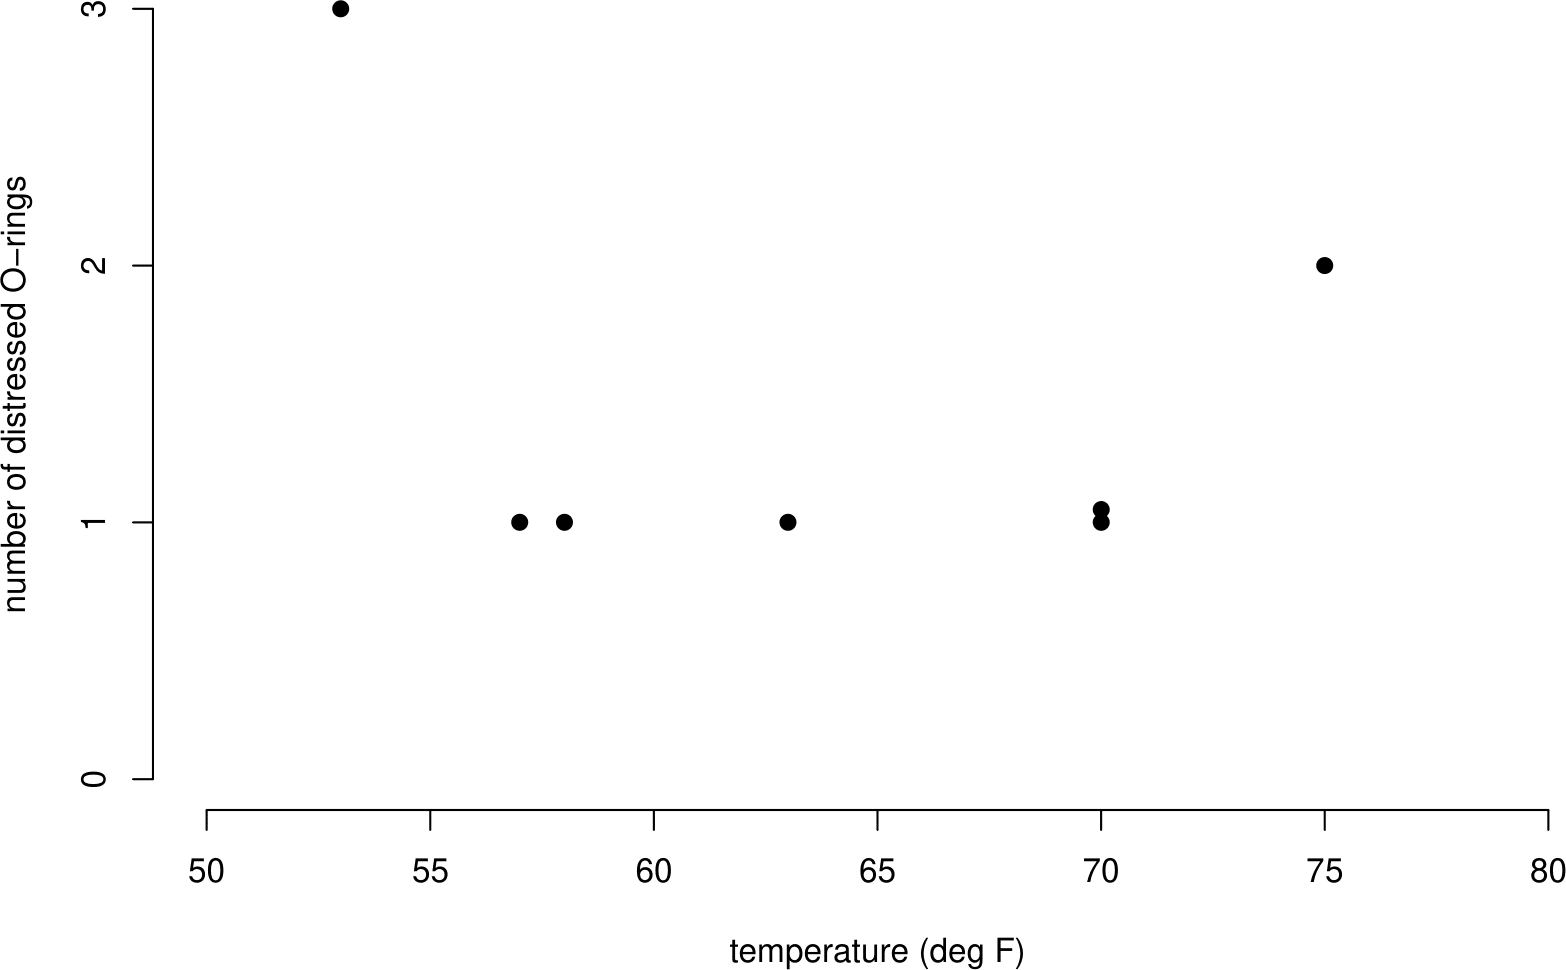
\includegraphics[width=0.75\linewidth]{images/shuttle1} 

}

\caption{Number of damaged O-rings plotted against temperature, for flights prior to 28/01/1986. Flights showing no incidents of distress have been omitted.  No clear association between the number of distressed O-rings and temperature is evident.}\label{fig:shuttle1}
\end{figure}

Flights giving zero incidents of thermal distress were not included in the graph. This was because it was felt that these flights did not contribute any information about the temperature effect. When the complete dataset (see Table \ref{tab:tabshuttle2} and Figure \ref{fig:shuttle2}) is examined it is clear that these flights \textbf{do} contribute extra information.

\begin{table}

\caption{\label{tab:tabshuttle2}Complete space shuttle data.  Number of damaged O-rings (out of a total of 6) for launches at a given temperature}
\centering
\begin{tabular}[t]{rllr}
\toprule
flight & date & damaged & temperature\\
\midrule
1 & 21/04/1981 & 0 & 66\\
2 & 12/11/1981 & 1 & 70\\
3 & 22/03/1982 & 0 & 69\\
4 & 11/11/1982 & 0 & 68\\
5 & 04/04/1983 & 0 & 67\\
\addlinespace
6 & 18/06/1983 & 0 & 72\\
7 & 30/08/1983 & 0 & 73\\
8 & 28/11/1983 & 0 & 70\\
9 & 03/02/1984 & 1 & 57\\
10 & 06/04/1984 & 1 & 63\\
\addlinespace
11 & 30/08/1984 & 1 & 70\\
12 & 05/10/1984 & 0 & 78\\
13 & 08/11/1984 & 0 & 67\\
14 & 24/01/1985 & 3 & 53\\
15 & 12/04/1985 & 0 & 67\\
\addlinespace
16 & 29/04/1985 & 0 & 75\\
17 & 17/06/1985 & 0 & 70\\
18 & 29/07/1985 & 0 & 81\\
19 & 27/08/1985 & 0 & 76\\
20 & 03/10/1985 & 0 & 79\\
\addlinespace
21 & 30/10/1985 & 2 & 75\\
22 & 26/11/1986 & 0 & 76\\
23 & 21/01/1986 & 1 & 58\\
24 & 28/01/1986 & ? & 31\\
\bottomrule
\end{tabular}
\end{table}

\begin{figure}

{\centering 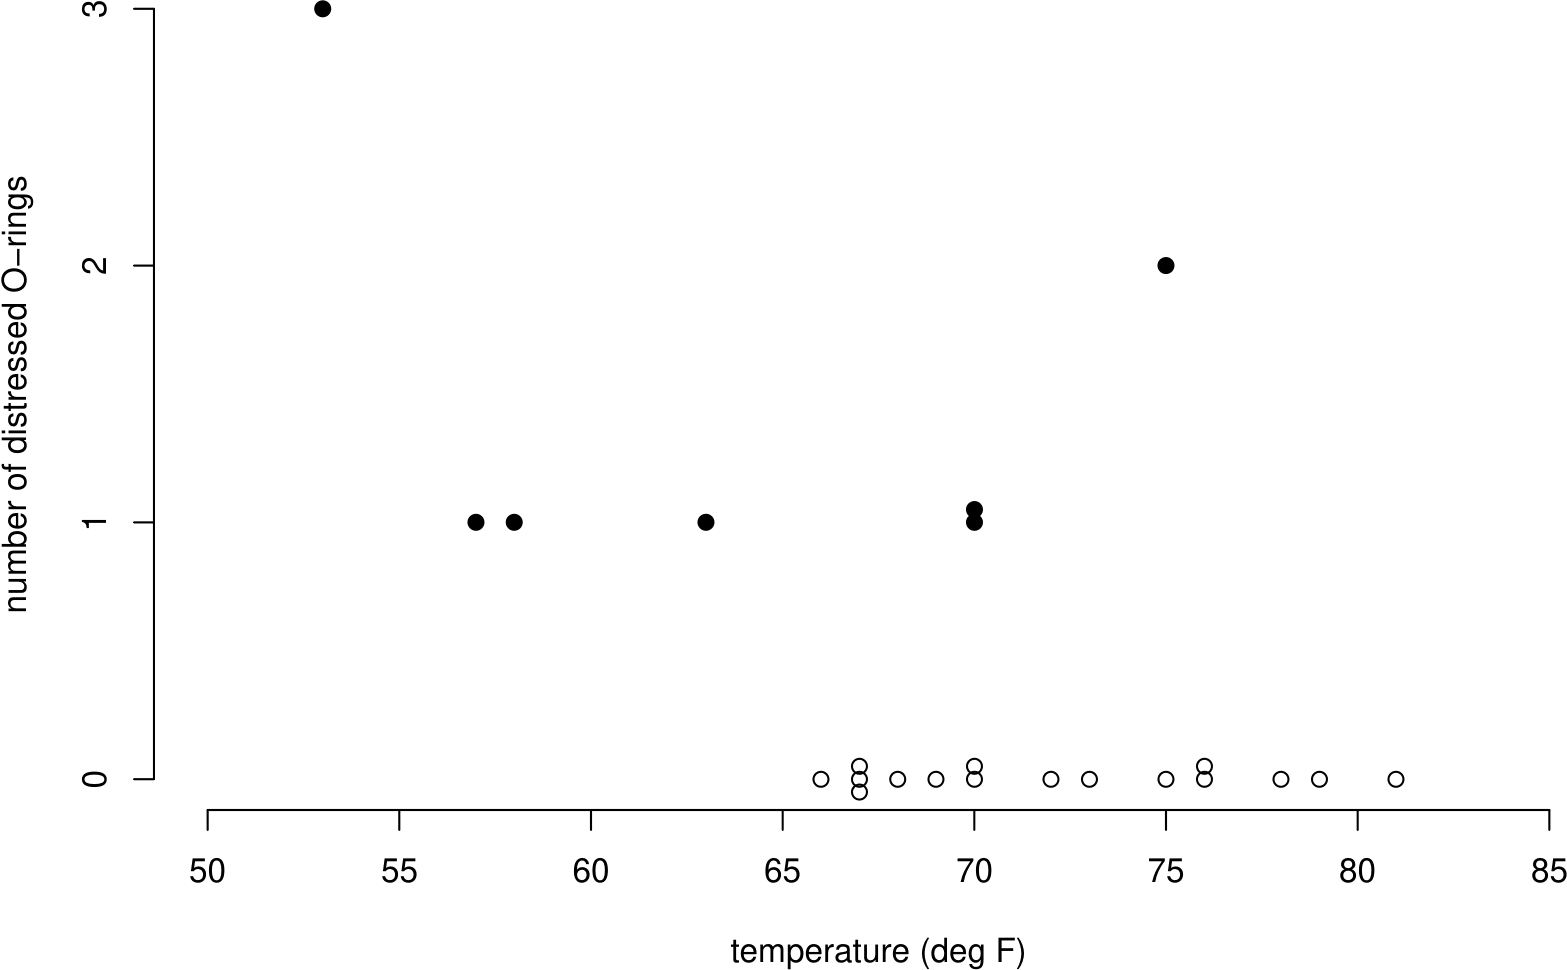
\includegraphics[width=0.75\linewidth]{images/shuttle2} 

}

\caption{Number of damaged O-rings plotted against temperature, for flights prior to 28/01/1986. Flights showing no incidents of distress have been included as hollow circles.  A clear negative association between the number of distress O-rings and temperature is evident.}\label{fig:shuttle2}
\end{figure}

The enquiry into the Challenger accident concluded that a more careful analysis of the O-ring data would have revealed the apparent effect of temperature on O-ring performance.

What can we learn from this example?

\begin{itemize}
\tightlist
\item
  Data analyses can have life and death consequences. Statisticians can be very important people!\\
\item
  Statistical analyses should use \textbf{all} the data. In this example only a non-random sample of the data are used. Removing some of the data had dire consequences. Values of zero are still data.
\item
  It is dangerous to extrapolate beyond the range of your data. No data were available below 50\(^\circ\)F. The forecast temperature of 31\(^\circ\)F was much lower than this.
\end{itemize}

After the accident \citet{shuttle} estimated the probability of a catastropic O-ring failure (that is, one that would cause an explosion) at 31\(^\circ\)F to be at least 0.13, which is large considering that seven lives were at stake. {[}To quantify their \textbf{uncertainty} they estimate that the probability is 90\% certain to be between 0.03 and 0.37.{]} However, it should certainly be made clear that this estimate may not be at all reliable. For example, it could be that as temperature decreases below 50\(^\circ\)F the risk of an accident increases much more quickly than the statistical analysis suggests.

The plot in Figure \ref{fig:shuttle3} gives you an idea of one of the analyses that \citet{shuttle} carried out. The sample proportions
of O-rings showing thermal distress (number of O-rings showing distress divided by 6) are plotted against temperature. Also plotted is a smooth curve fitted to these data. {[}This analysis is beyond scope of STAT0002/0003. You may study this type of model in STAT0023.{]}

\begin{figure}

{\centering 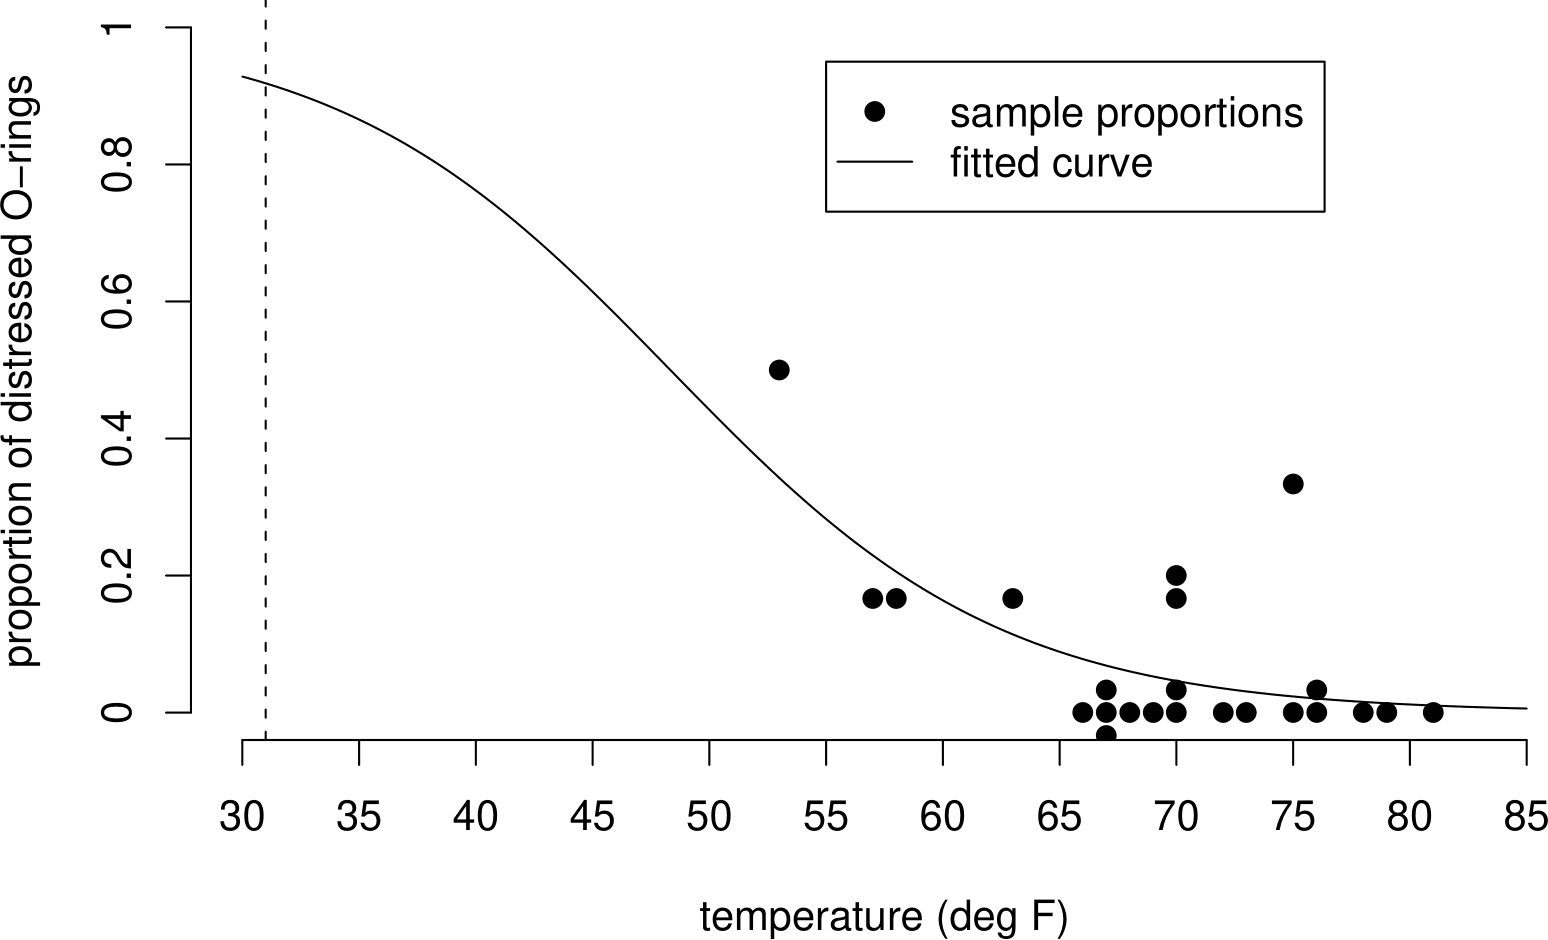
\includegraphics[width=0.75\linewidth]{images/shuttle3} 

}

\caption{Proportion of O-rings showing some thermal distress plotted against temperature, with fitted logistic curve.  The fitted curve reflects the apparent negative association between this proportion and temperature.}\label{fig:shuttle3}
\end{figure}

\hypertarget{uncertainty}{%
\subsection{Uncertainty}\label{uncertainty}}

Suppose there is a true curve, of the same general type as the one in Figure \ref{fig:shuttle3}, which describes how the probability that an O-ring is damaged depends on temperature. We use the NASA test flight data to guess, or \textbf{estimate} the exact shape of this true curve. The curve in figure \ref{fig:shuttle3} is \textbf{not} the true curve, it is an \textbf{estimate} of the true curve based on these data.

If NASA repeated their launches, at exactly the same temperatures, these new data on the number of damaged O-rings would not be the same as the old data and the shape of the new estimated curve would be different from the shape of the old estimated curve. It may be that these 2 curves are quite similar or it could be that they are very different. We could ask them, very politely, repeat this process many times to get a large number of different sets of data. Each set of data produces an estimated curve.

The dataset (and its estimated curve) we have is just one of many possible datasets that could be produced. We can imagine picking this dataset (and curve) at random from a big bag of possible datasets (and curves). These ideas are summarised in Figure \ref{fig:shuttlediagram}.

\begin{figure}

{\centering 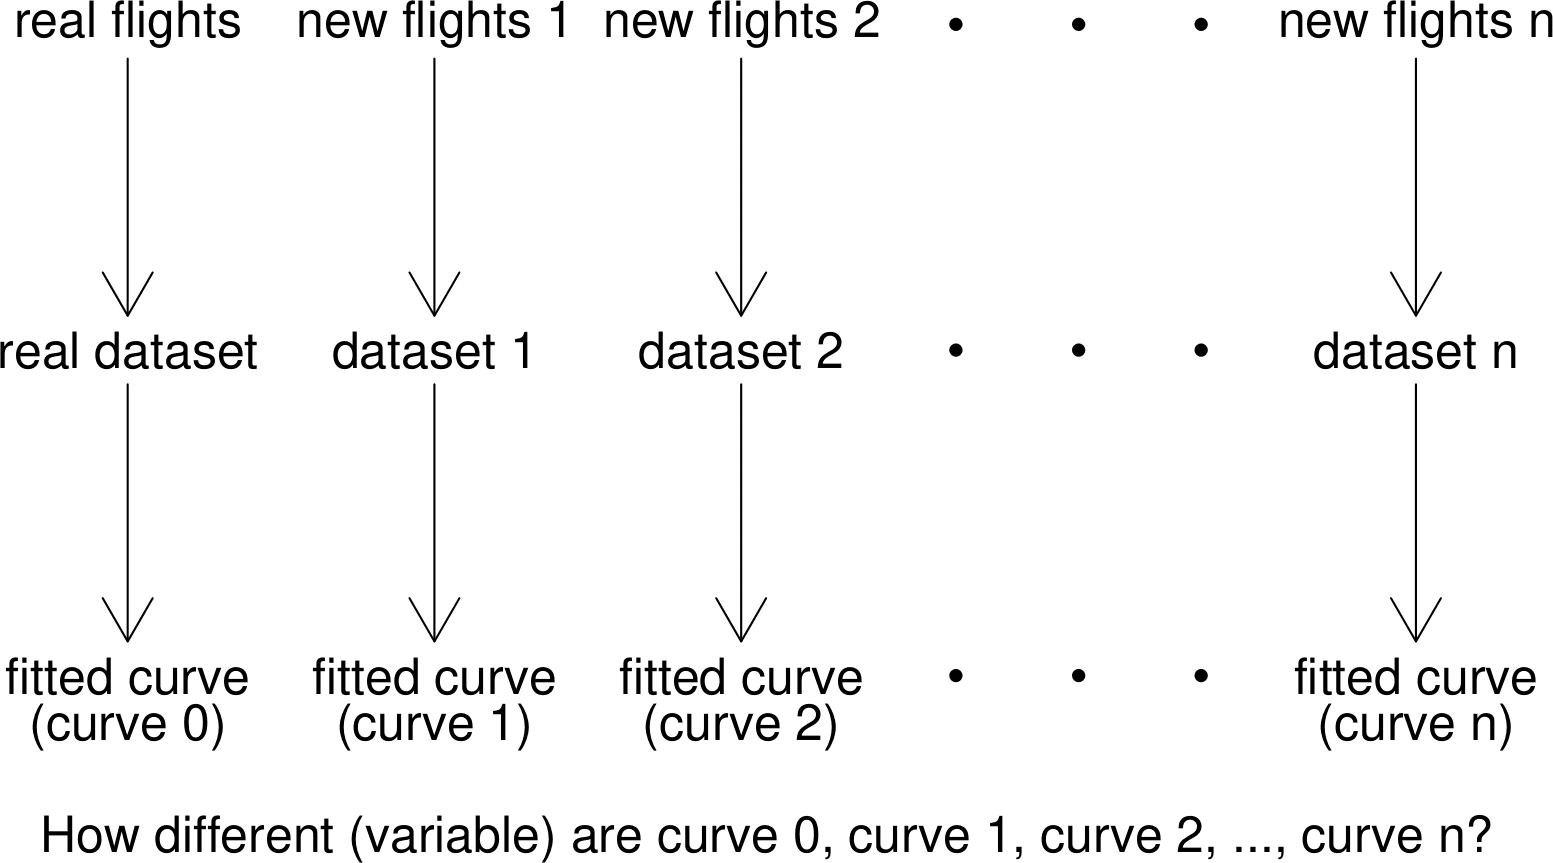
\includegraphics[width=0.75\linewidth]{images/shuttle_diagram} 

}

\caption{Diagram to illustrate the idea of repeating an experiment many times.  Each simulated set of flights leads to its own dataset and fitted logistic curve.}\label{fig:shuttlediagram}
\end{figure}

Suppose that the estimated curves from the possible datasets are very similar to each other. We say that their \textbf{variability} is small. If this is the case then it doesn't matter much which dataset we picked from the big bag of possible datasets: the results are similar for all datasets. Therefore, we can be fairly certain that the results we got from the dataset we have are close to the truth. Therefore the \textbf{uncertainty} surrounding the results is small.

On the other hand, if the estimated curves from the possible datasets are very different to each other then their \textbf{variability} is large. If this is the case then the results will be very different depending on which dataset we pick. Therefore, it is possible that the results we got from the dataset are very far from the truth. Therefore the \textbf{uncertainty} about the results is large.

We can see that \textbf{variability} and \textbf{uncertainty} are closely related. Small variability tends to produce small uncertainty, whereas large variability tends to produce large uncertainty. As we might expect the amount of data, (or, more precisely, the amount of \textbf{information} in the data) matters. Large datasets, with lots of information, tend to produce small variability in the results and therefore small uncertainty. Small datasets, with small amounts of information, tend to produce large variability in the results and therefore large uncertainty.

So, how can we quantify how much uncertainty there is in the space shuttle example? It is unlikely that NASA will carry out all their launches again just for us. However, it is possible for us to produce (\textbf{simulate}) on a computer our own, fake, datasets using the estimated curve in Figure \ref{fig:shuttle3}. If this curve (and the assumptions used to produce it) are correct, this is equivalent to NASA carrying out more test flights: the simulated datasets have exactly the same statistical properties as the real dataset. In summary, we

\begin{itemize}
\tightlist
\item
  create a large number of fake (\textbf{simulated}) datasets;
\item
  for each dataset we estimate a curve to describe how the probability of O-ring damage depends on temperature;
\item
  examine how much the curves, and the estimate of probability at different temperatures vary between the simulated datasets.
\end{itemize}

Figure \ref{fig:shuttlesimcurves} shows 50 simulated curves and the curve estimated from the real data.

\begin{figure}

{\centering 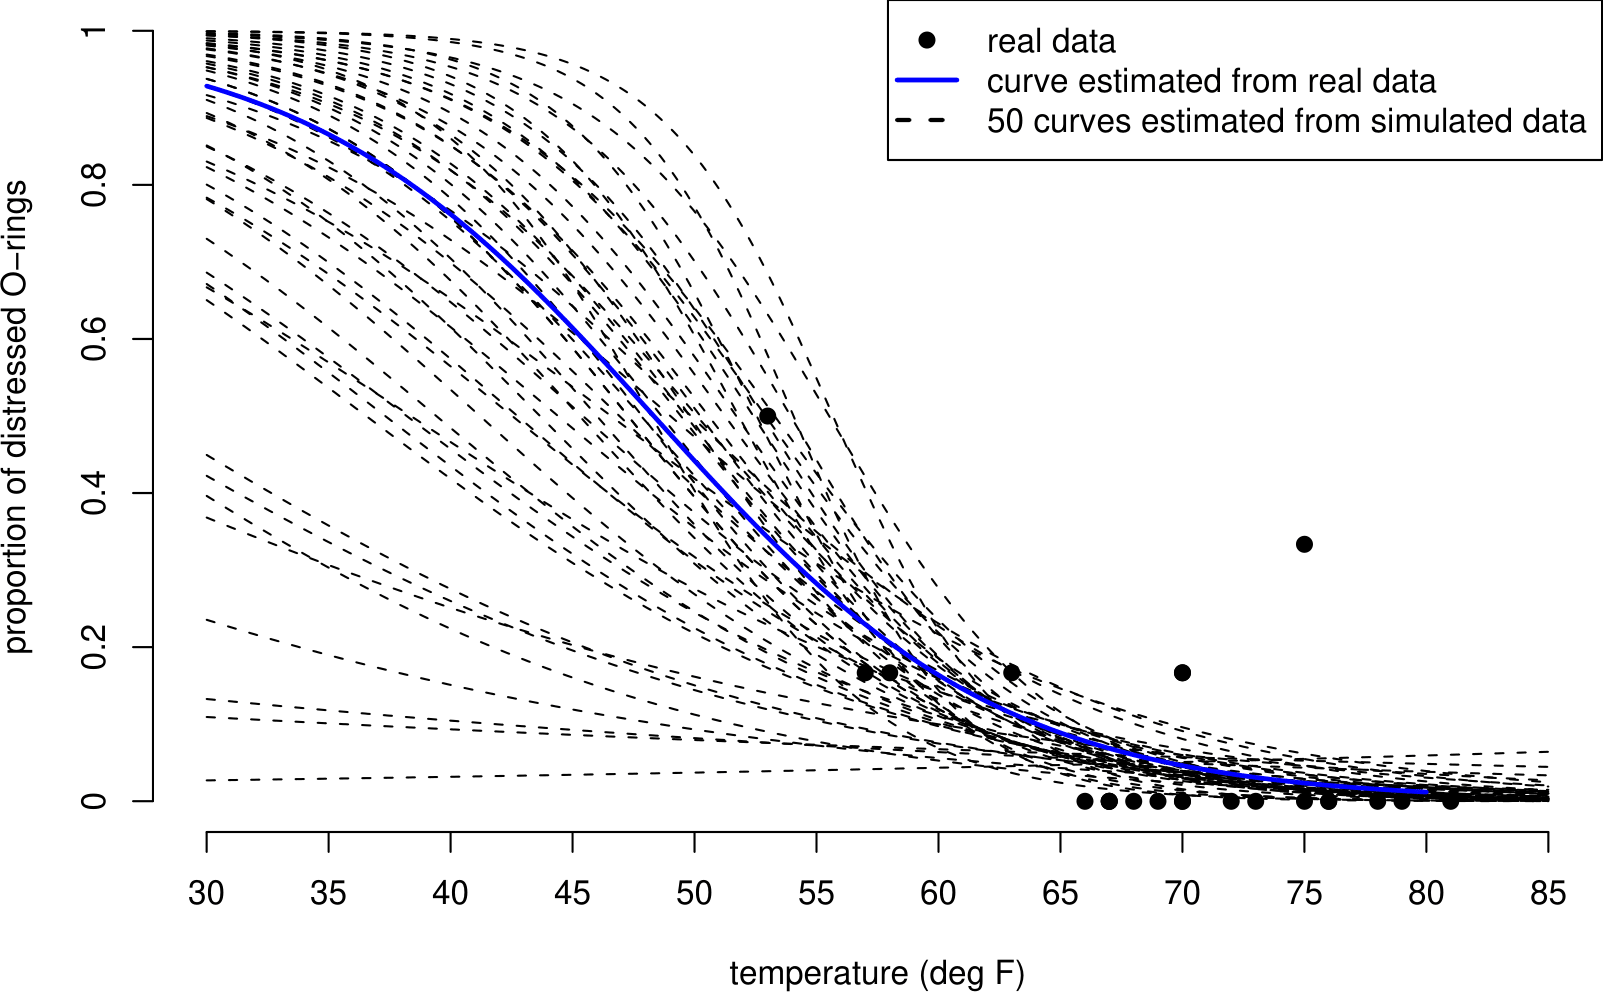
\includegraphics[width=0.75\linewidth]{images/shuttle_simcurves} 

}

\caption{50 curves fitted to simulated shuttle test flight data. The curves are similar over the range of temperatures observed in the data (53 to 81 degrees F), but vary greatly for lower temperatures, such as 31 degrees F.}\label{fig:shuttlesimcurves}
\end{figure}

There is a lot of variability in these curves. Notice that the curves are quite close to each other for high temperatures - where we have some data - but that they are very spread out for low temperatures - where we have no data. This is confirmed by figure \ref{fig:shuttlesim} which shows how the estimated probability of O-ring damage depends on temperature.

\begin{figure}

{\centering 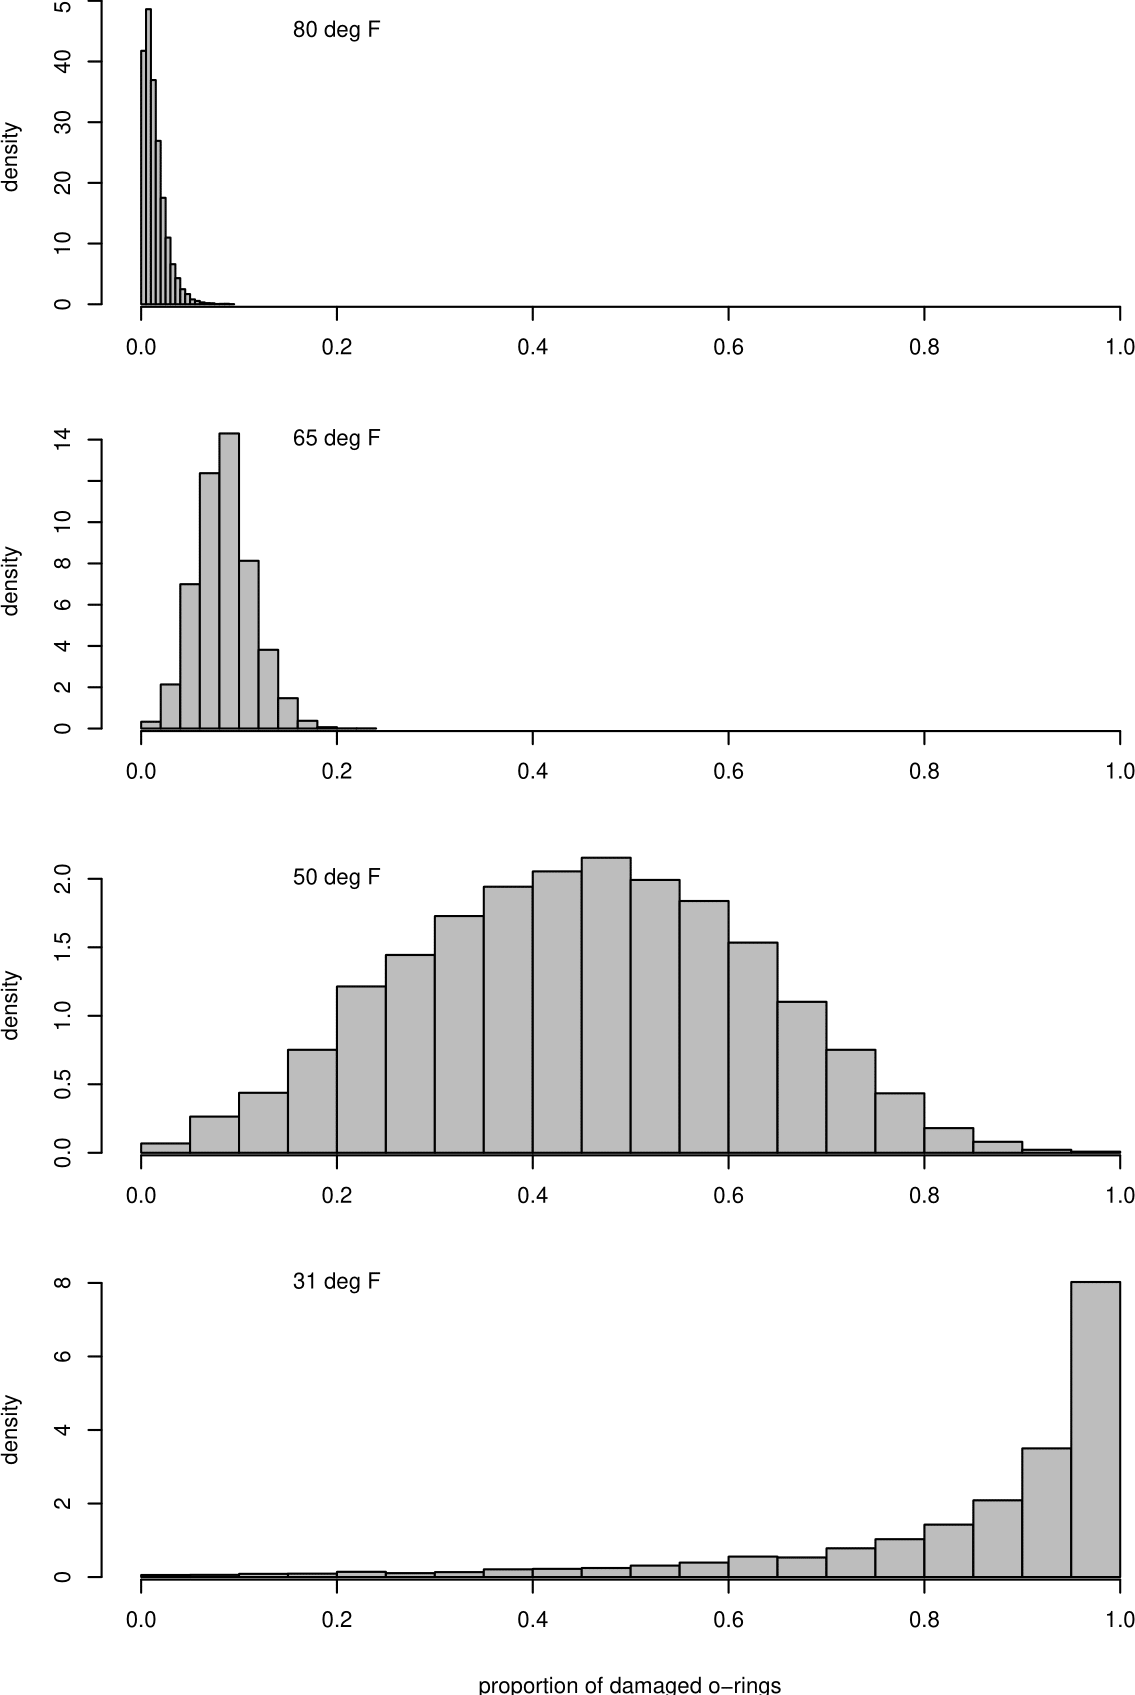
\includegraphics[width=0.75\linewidth]{images/shuttle_sim} 

}

\caption{Histograms of estimated probabilities of O-ring damage at different temperatures.}\label{fig:shuttlesim}
\end{figure}

There is a large amount of uncertainty about the esimatated probabilities, particularly at 31\(^\circ\)F, where it really mattered.

To show the effect of sample size (the size of the dataset) we simulate datasets which are larger than the real dataset and see how much the curves fitted to these data vary between the datasets. Figure \ref{fig:shuttlesimcurves10} shows the estimated curves from 50 datasets, each of which is 10 times the size of the real dataset. Figure \ref{fig:shuttlesimcurves100} shows curves for datasets which are 100 times the size of the original dataset. As the sample size increases the variability decreases and so the uncertainty decreases.

\begin{figure}

{\centering 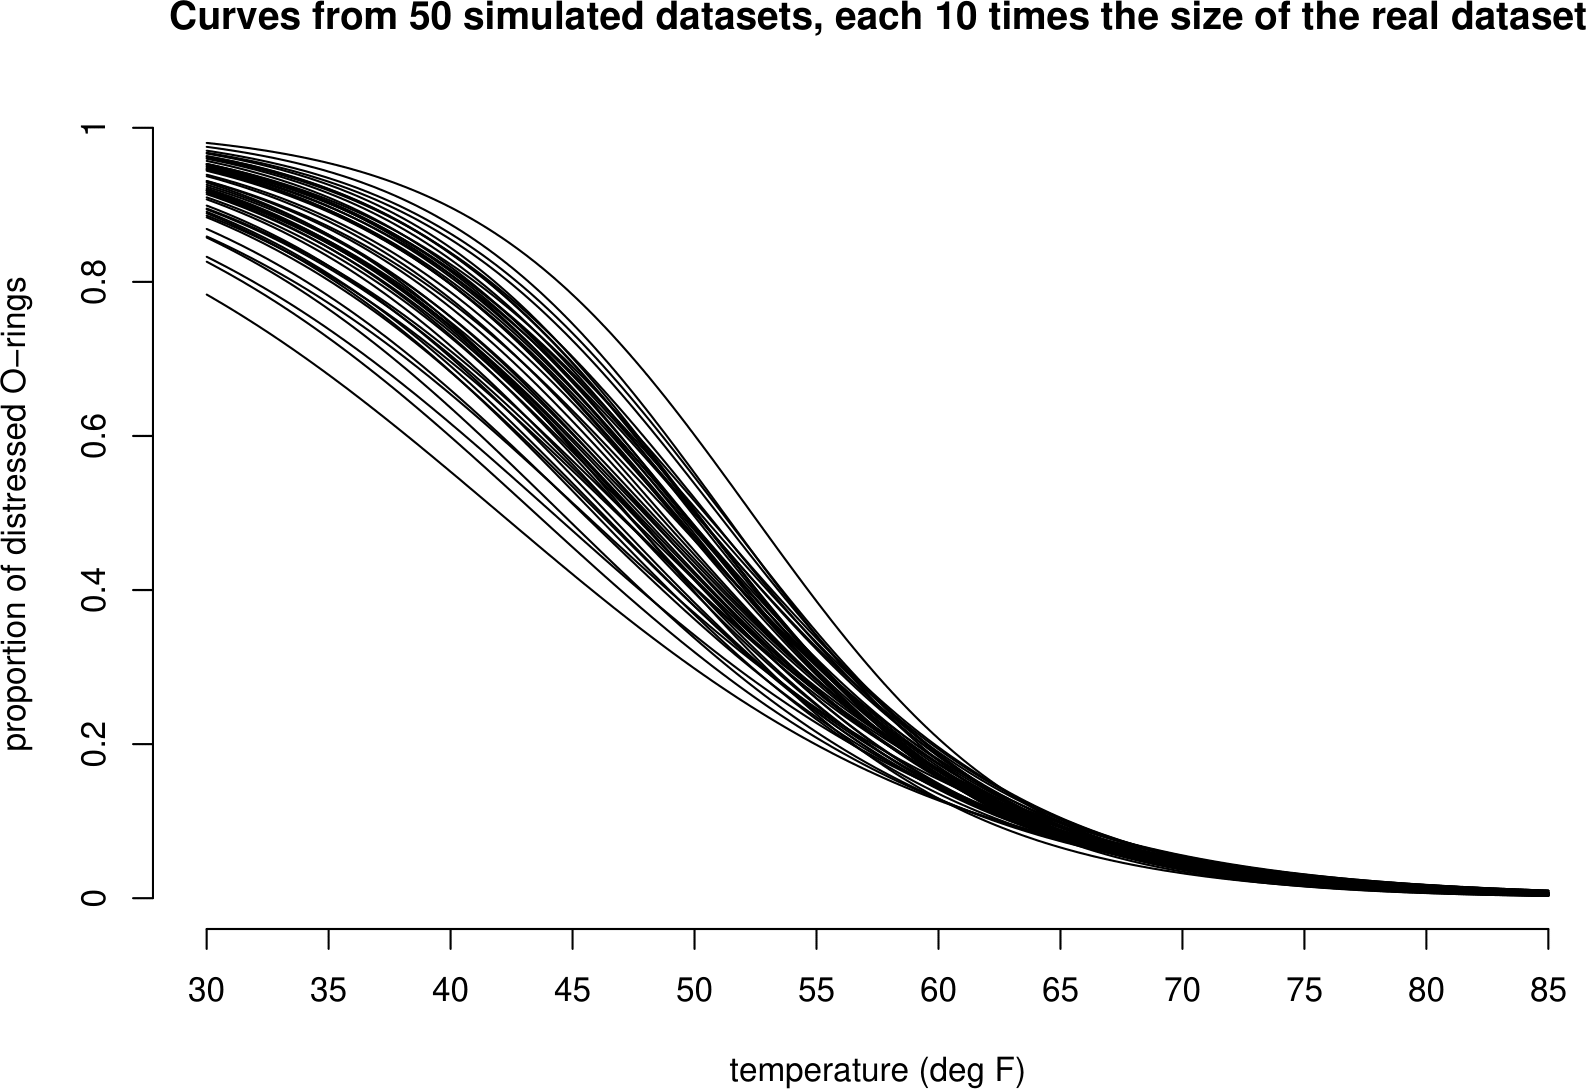
\includegraphics[width=0.75\linewidth]{images/shuttle_simcurves10} 

}

\caption{50 curves fitted to simulated shuttle test flight datasets that are each 10 times the size of the real dataset.  In comparision to the curves based on the real dataset these curves vary less, but are still most variable for low temperatures.}\label{fig:shuttlesimcurves10}
\end{figure}

\begin{figure}

{\centering 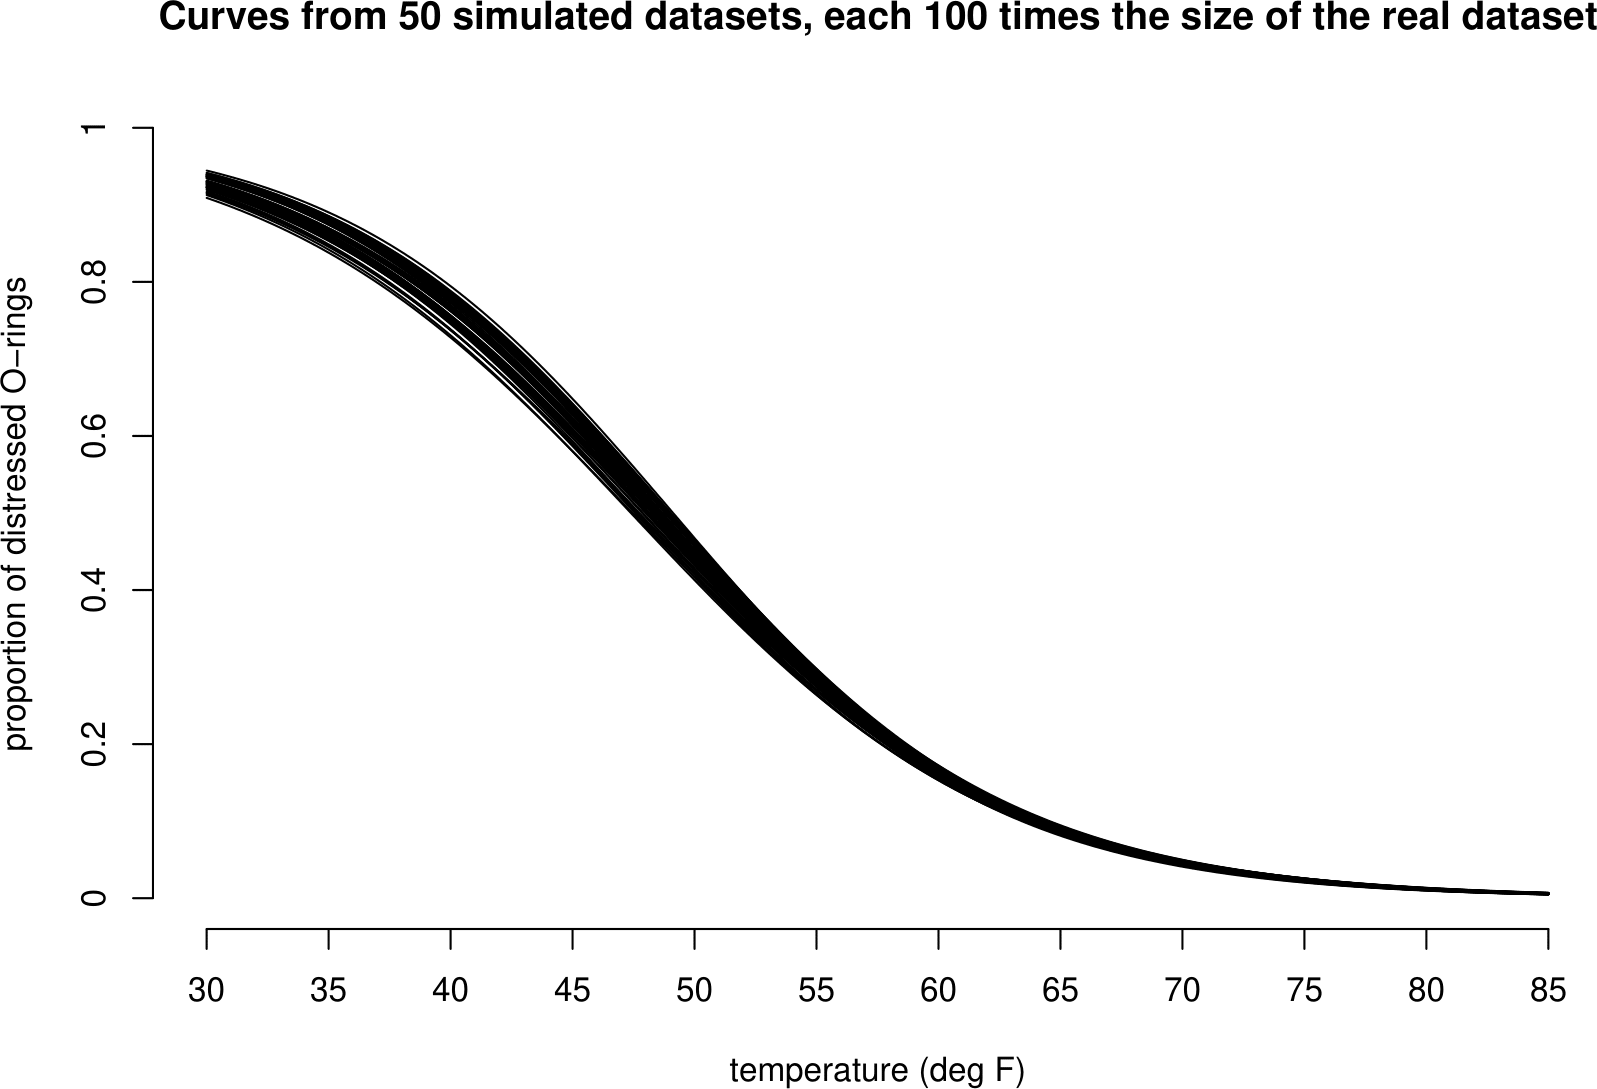
\includegraphics[width=0.75\linewidth]{images/shuttle_simcurves100} 

}

\caption{50 curves fitted to simulated shuttle test flight datasets that are each 100 times the size of the real dataset. In comparision to the curves based on the real dataset these curves vary much less, but are still most variable for low temperatures.}\label{fig:shuttlesimcurves100}
\end{figure}

\hypertarget{a-very-brief-introduction-to-stochastic-simulation}{%
\section{A very brief introduction to stochastic simulation}\label{a-very-brief-introduction-to-stochastic-simulation}}

This section contains words that we will not define until later in the course. Further information about stochastic simulation is available from the Stochastic Simulation section of the STAT0002 Moodle page.

In Statistics it is common to assess a statistical method based on how well it would perform if used repeatedly on a large number of new datasets, where we imagine that the new datasets have exactly the same statistical properties as the real data. In some cases it is possible to do this using mathematics. Alternatively, we can use a computer to produce some fake (simulated) datasets from a model that has been fitted to the real data. How can we do this?

Stochastic (stochastic simply means ``involving randomness'') simulation is based on the ability to generate a random number \(u\) between 0 and 1. Stochastic simply means ``involving randomness''. Your pocket calculator probably has a button to do this, perhaps called RAN\#. It is possible to transform this number \(u\) so that it looks like it has been drawn from the distribution required, e.g.~a binomial distribution or a normal distribution. If we produce a sequence \(u_1, u_2, \ldots, u_n\) of random numbers between 0 and 1 and transform them appropriately, then the transformed values will look like a random sample from the distribution required. Of course, because these values are produced by rule implemented by a computer they are not really random. However, if the rule is designed carefully, these values are close enough to being a random sample for our purposes.

For the purposes of the space shuttle experiment we simply need to simulate a 1 (O-ring distressed) with probability \(p\), and a 0 (0-ring not distressed) with probability \(1-p\). This is easy. If \(U\) is a random number between 0 and 1 then the probability that \(U < p\) is \(p\). Therefore, we define

\begin{equation}
X = 
\begin{cases} 
1 & \text{if } U < p, \\
0 & \text{if } U \geq p.
\end{cases}
\label{eq:xbin}
\end{equation}

For \(p=1/2\) this is like using a computer to flip an unbiased coin.

To simulate a fake space shuttle dataset we do the following for each of the 23 flights:

\begin{enumerate}
\def\labelenumi{\arabic{enumi}.}
\tightlist
\item
  set \(p\) to be the value of the fitted curve in Figure \ref{fig:shuttle3} corresponding to the flight temperature;
\item
  generate 6 random numbers \(u_1, \ldots, u_6\) between 0 and 1;
\item
  calculate \(x_1, \ldots, x_6\) using equation \eqref{eq:xbin};
\item
  calculate \(y=x_1+\cdots+x_6\), the total number of distressed O-rings.
\end{enumerate}

We have assumed that the 6 O-rings have the same probability of becoming distressed and are distressed independently of each other. In Chapter \ref{rvs} we will see that \(y\) is a value simulated from a binomial(6, \(p\)) distribution. We will use simulation several times in STAT0002 to study properties of statistical methods. All you need to know is that we can use a computer to produce fake data that look like they come from a certain probability distribution.

\hypertarget{descriptive-statistics}{%
\chapter{Descriptive Statistics}\label{descriptive-statistics}}

The first important step in any data analysis is to \textbf{describe} the
available data. This is often called an \textbf{exploratory} or \textbf{initial} data analysis. It is normally not possible to just look at the dataset, especially if it is large, and just see any interesting structures. The task of a statistician is therefore to \textbf{extract} and \textbf{condense} the relevant information -- what is relevant will depend on the aim of the analysis. Some of the standard methods to do so are addressed in the next sections. Despite all the technicalities, always remember that the numbers / figures / plots produced for data must be \textbf{interpreted with regard to the problem or question at hand}, that is, always ask yourself ``what does this number / plot mean?''.

Before embarking on a formal statistical analysis of the data we should look at summaries of the data such as graphs, tables and summary statistics. This can be important to

\begin{enumerate}
\def\labelenumi{\arabic{enumi}.}
\tightlist
\item
  reveal problems with, or errors in, the data;
\item
  get a `feel' for the data;
\item
  identify interesting features of the data, e.g.~is treatment A very
  obviously better at treating a disease than treatment B?;
\item
  suggest how the data should be analysed;
\item
  present conclusions.
\end{enumerate}

In some cases the data summaries make it very clear what is going on and may
make more formal methods of statistical analysis unnecessary.

\hypertarget{types-of-data}{%
\section{Types of data}\label{types-of-data}}

Before analysing data it is important to consider what \textbf{type} they are. This will affect which statistics it is sensible to calculate, which graphs it is sensible to plot and which of the simple distributions we will study in Chapter \ref{simple} might be used for these data.

\hypertarget{qualitative-or-categorical-data}{%
\subsection{Qualitative or categorical data}\label{qualitative-or-categorical-data}}

Items are assigned to \textbf{groups} or \textbf{categories} based on some \textbf{qualitative} property. Examples:

\begin{itemize}
\tightlist
\item
  Hair colour: blonde, brown, red, black etc.
\item
  Smoking status: smoker, non-smoker;
\item
  Severity of illness: none, mild, moderate, severe;
\item
  Degree class: 3, 2ii, 2i, 1.
\end{itemize}

The data are \textbf{labels}: if numbers are assigned to the categories (e.g.~
0=smoker, 1=non-smoker) the numbers chosen do not mean anything in themselves.

Categorial data can be classified as either

\begin{itemize}
\tightlist
\item
  \textbf{nominal}: the categories are unordered, e.g.~hair colour, smoking status;
\item
  \textbf{ordinal}: the categories are ordered, e.g.~severity of illness, degree class.
\end{itemize}

An important special case is \textbf{binary} data: categorical data with only 2 categories. These data can be nominal (e.g.~male, female) or ordinal (e.g.~small, large).

Nominal data: describe by (relative) frequencies. It is sensible to quote the mode, but not the mean or median.

Ordinal data: It is sensible to quote the mode or median, but not the mean.

\hypertarget{quantitative-or-numerical-data}{%
\subsection{Quantitative or numerical data}\label{quantitative-or-numerical-data}}

Items are measured in some way based on some \textbf{quantitative} property. This produces a one, or more, \textbf{numbers}. Examples:

\begin{itemize}
\tightlist
\item
  Time, in hours;
\item
  Height, in cm;
\item
  Age, in years;
\item
  Number of damaged O-rings (see space shuttle investigation);
\item
  Number of births on one day at a particular hospital;
\item
  Number of units passed in first year.
\end{itemize}

Numerical data can be classified as either

\begin{itemize}
\tightlist
\item
  \textbf{Discrete}. Only certain values are possible (there are gaps between the possible values), e.g.~number of damaged O-rings, number of births, number of units passed in first year (0, 0.5, 1, 1.5, 2, 2.5, 3, 3.5, 4);
\item
  \textbf{Continuous}. In theory, \textbf{any} value within an interval of the real line
  is possible, e.g.~time, height, age.
\end{itemize}

Often discrete data are \textbf{counts}. Continuous data usually come from measurement. In practice continuous data are recorded discretely, e.g.~to two decimal places.

\hypertarget{interval-data-and-ratio-data}{%
\subsubsection*{Interval data and ratio data}\label{interval-data-and-ratio-data}}
\addcontentsline{toc}{subsubsection}{Interval data and ratio data}

Quantitative data can be further classified as \textbf{interval} or \textbf{ratio}. Both interval data and ratio data have the property that an increase of 1 unit means the same whether it is from, say, 1 to 2 or from 10 to 11. However,

\begin{itemize}
\tightlist
\item
  a ratio scale has a natural zero, for example, temperature measured in degrees Kelvin;
\item
  an interval scale does not have a natural zero, for example temperature
  measured in Fahrenheit.
\end{itemize}

Ratios are only meaningful on a ratio scale. For example,

\begin{itemize}
\tightlist
\item
  IQ: A zero IQ does not exist. A person with an IQ of 120 is not twice as intelligent as a person with an IQ of 60. Therefore, IQs are interval data.
\item
  Income: A zero income does exist. A person whose take-home income is \pounds 20,000 does earn twice as much as some whose take-home income is \pounds 10,000.Therefore, incomes are ratio data.
\end{itemize}

\hypertarget{describing-distributions}{%
\section{Describing distributions}\label{describing-distributions}}

In describing the distribution of one variable the following it is important to
examine the following.

\begin{enumerate}
\def\labelenumi{\arabic{enumi}.}
\tightlist
\item
  \textbf{Location / average / central tendency of the data}. Where is the centre of the distribution? What is a typical value?\\
\item
  \textbf{Spread / variability / dispersion / scale}. How \textbf{variable} are the data? How far are they spread out?
\item
  \textbf{Shape}. What shape is the distribution of the data? In particular, is it \textbf{symmetric} or \textbf{skewed}, and if skewed, which way? A long tail to the right is called \textbf{positive skew} (or right skew or skewed to the right). A long tail to the left is known as a \textbf{negative skew} (or left skew or skewed to the left). Positive skew is much more common than negative skew. Figure \ref{fig:shapes} gives some examples of shapes of symmetric, positive skew and negative skew distributions. In addition to being symmetric the plot in the top left of Figure \ref{fig:shapes} of figure is bell-shaped. This shape is the shape of a \textbf{normal distribution} (see Section \ref{normal}). The normal distribution is an important distribution in Statistics. We may wish to decide whether the data look like they have come from a normal distribution.
\item
  \textbf{Outliers}. Are there any outliers, that is, observations that appear to be out of line with the pattern of the rest of the data? This issue can also be hard to judge. For example, with a small number of observations, it is difficult to distinguish between data from a heavily skewed distribution and data from a symmetric distribution with outliers. What constitutes an outlier depends on the context so there is no rigid rule for defining/detecting outliers. The intended statistical analysis also matters. We will consider how to deal with outliers (in the context of linear regression) in Section \ref{outliers}.
\item
  \textbf{Is there anything else to report?} Note any \textbf{unusual features}
  about the data. Are there particular numbers which appear more often than we could expect? Do the data separate into groups?
\end{enumerate}

\begin{figure}

{\centering 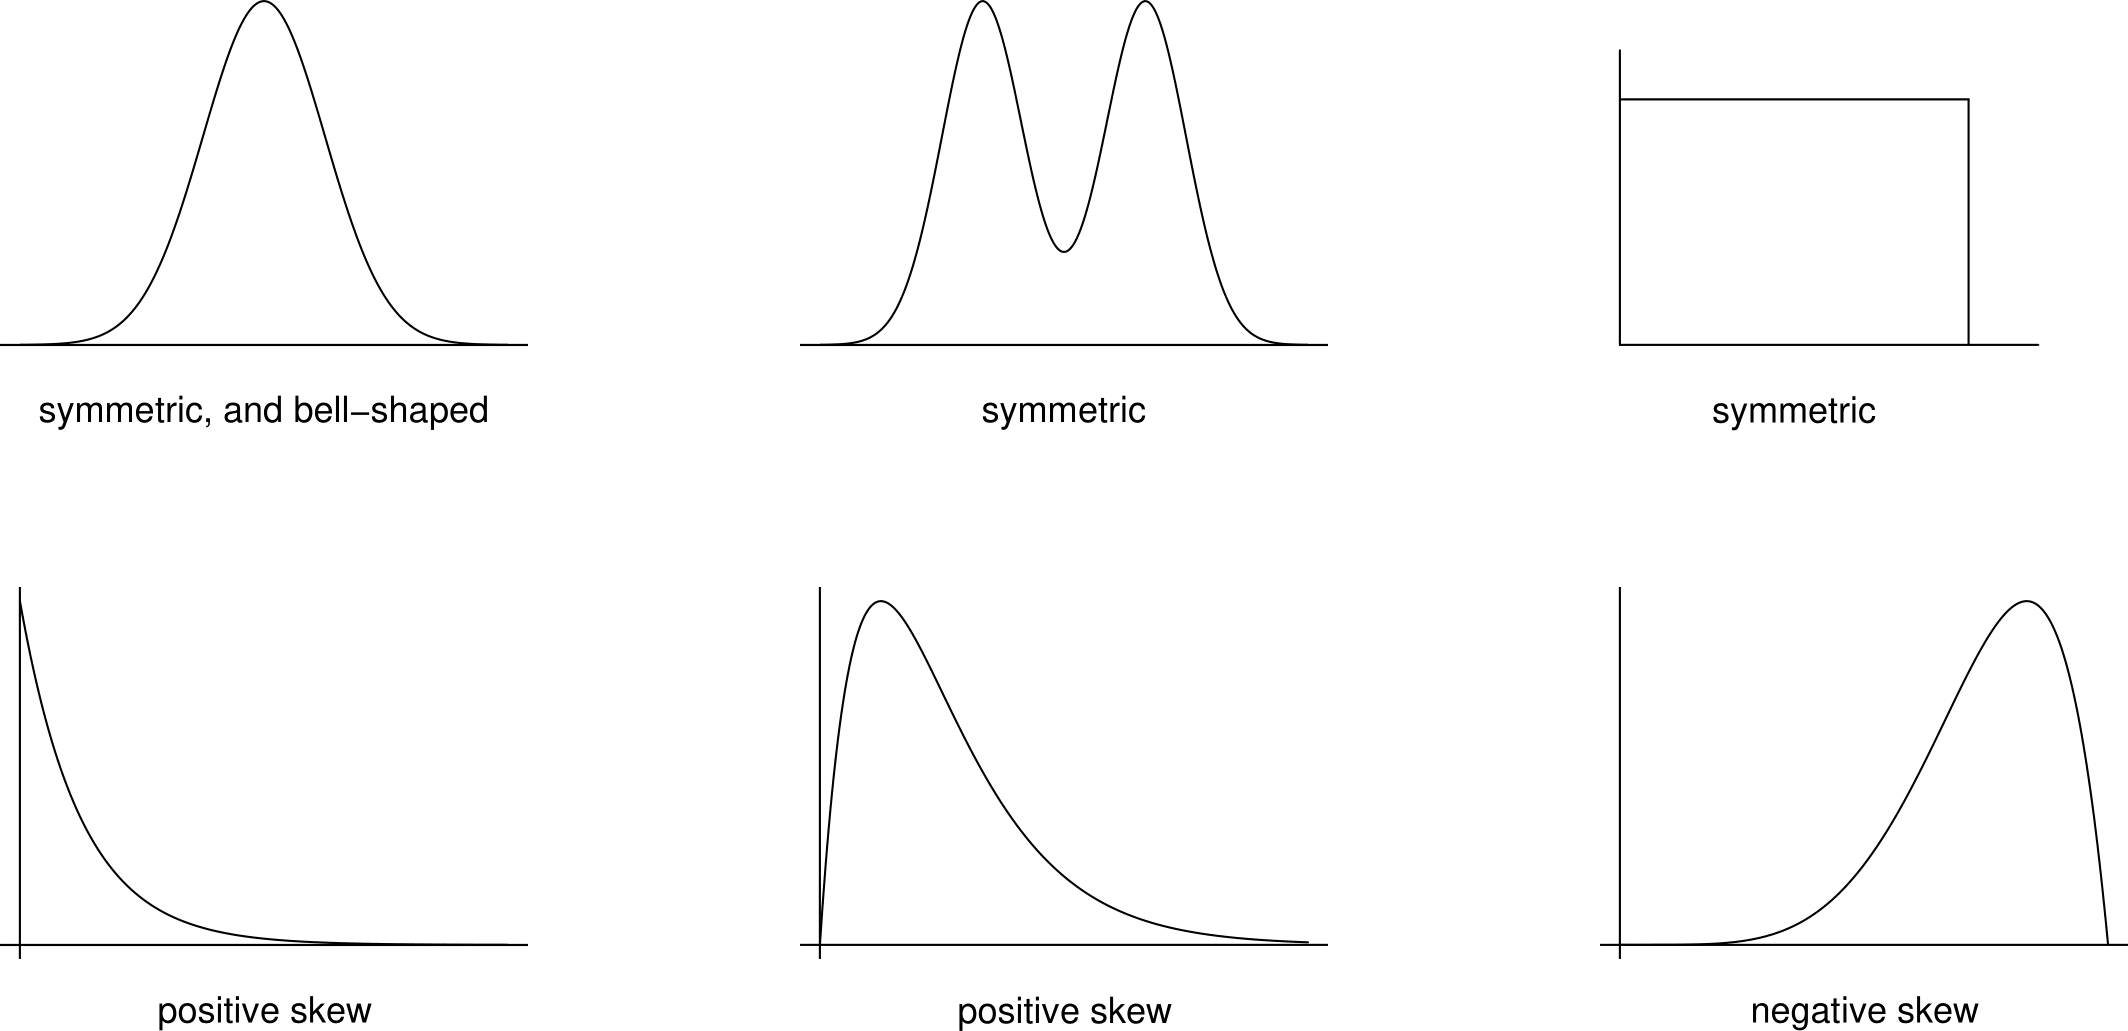
\includegraphics[width=0.75\linewidth]{images/shapes} 

}

\caption{Examples of shapes of symmetric, positively skewed and negatively skewed distributions.}\label{fig:shapes}
\end{figure}

We will look at 3 ways basic tools which are used to describe and summarise data: summary statistics, tables and graphs. We can use a combination of these. For example summary statistics may be presented in a table or a graph. Carefully produced graphs are often the best way to describe, explore and summarise a set of data. Summary statistics reduce the data to a small set of numbers. Tables can retain more information but do not work well for datasets which are large or have many variables. In contrast graphs can show most, if not all, the information in the data and reveal complex relationships.

\hypertarget{example-oxford-births-data}{%
\subsection*{Example: Oxford births data}\label{example-oxford-births-data}}
\addcontentsline{toc}{subsection}{Example: Oxford births data}

Table \ref{tab:taboxbirths} shows the times (in hours) spent by 95 women giving birth in the delivery suite of the John Radcliffe Hospital in Oxford during 1 week. These are ratio data. At first we ignore the fact that the data are recorded on different days.

\begin{table}

\caption{\label{tab:taboxbirths}Time (in hours) spent by each of 95 women giving birth at the John 
Radcliffe hospital in Oxford, UK, during a particular week.}
\centering
\begin{tabular}[t]{rrrrrrr}
\toprule
day1 & day2 & day3 & day4 & day5 & day6 & day7\\
\midrule
2.10 & 4.00 & 2.60 & 1.50 & 2.50 & 4.00 & 2.00\\
3.40 & 4.10 & 3.60 & 4.70 & 2.50 & 4.00 & 2.70\\
4.25 & 5.00 & 3.60 & 4.70 & 3.40 & 5.25 & 2.75\\
5.60 & 5.50 & 6.40 & 7.20 & 4.20 & 6.10 & 3.40\\
6.40 & 5.70 & 6.80 & 7.25 & 5.90 & 6.50 & 4.20\\
\addlinespace
7.30 & 6.50 & 7.50 & 8.10 & 6.25 & 6.90 & 4.30\\
8.50 & 7.25 & 7.50 & 8.50 & 7.30 & 7.00 & 4.90\\
8.75 & 7.30 & 8.25 & 9.20 & 7.50 & 8.45 & 6.25\\
8.90 & 7.50 & 8.50 & 9.50 & 7.80 & 9.25 & 7.00\\
9.50 & 8.20 & 10.40 & 10.70 & 8.30 & 10.10 & 9.00\\
\addlinespace
9.75 & 8.50 & 10.75 & 11.50 & 8.30 & 10.20 & 9.25\\
10.00 & 9.75 & 14.25 &  & 10.25 & 12.75 & 10.70\\
10.40 & 11.00 & 14.50 &  & 12.90 & 14.60 & \\
10.40 & 11.20 &  &  & 14.30 &  & \\
16.00 & 15.00 &  &  &  &  & \\
\addlinespace
19.00 & 16.50 &  &  &  &  & \\
\bottomrule
\end{tabular}
\end{table}

\hypertarget{summary-statistics}{%
\section{Summary Statistics}\label{summary-statistics}}

One way to summarise a dataset is to calculate numerical summaries called \textbf{summary statistics}. Summary statistics can be used as indicators of the location, spread and shape of the data (although looking at a plot can be more helpful).

\hypertarget{five-number-summary}{%
\subsection{Five number summary}\label{five-number-summary}}

A useful first impression of the distribution of quantitative or ordinal data is given by the a five number summary. As we will see later, the five number summary involves quantities called \textbf{sample quantiles}. These are estimates of theoretical quantities that we will study in Chapter \ref{rvs}. There is more than one way to calculate sample quantiles. For example, the R statistical package has 9 options in its \texttt{quantile()} function. The particular method given below is just one of these options.

If a dataset of observations, \(x_1,x_2,\ldots,x_n\), is arranged in order of size as \[ x_{(1)} \leq x_{(2)} \leq \cdots \leq x_{(n)}\] then the \textbf{sample median} is the `middle' value (halfway between \(x_{(1)}\) and \(x_{(n)}\)), that is,
\[ m=x_{(\frac{1}{2}(n+1))}\,.\]
The median is a measure of location.

Informally, we can think of the \textbf{sample lower quartile} as the sample median of the lower half of the data, or, equivalently, as the value that divides the lower 25\% of the data from the rest of the data. One way to estimate this is
\[ q_L=x_{(\frac{1}{4}(n+1))} \,.\]
Similarly, we can think of the \textbf{sample upper quartile} as the sample median of the upper half of the data, which we could estimate using
\[ q_U=x_{(\frac{3}{4}(n+1))}\,.\]
If \(m, q_L\) or \(q_U\) do not correspond directly with one of the observations
then we can use linear interpolation. Suppose that \(n=44\). Then we could calculate the sample median using
\[x_{(22.5)}=x_{(22)}+\frac12\left(x_{(23)}-
x_{(22)}\right)=\frac{x_{(22)}+x_{(23)}}{2}, \]
the sample lower quartile using
\[ x_{(11.25)}=x_{(11)}+\frac14\left(x_{(12)}-
x_{(11)}\right)=\frac34\,x_{(11)}+\frac14\,x_{(12)}, \]
and the sample upper quartile using
\[x_{(33.75)}=x_{(33)}+\frac34\left(x_{(34)}-
x_{(33)}\right)=\frac14\,x_{(33)}+\frac34\,x_{(34)}.\]
This is not the only possibility: you may find that different methods are used in some textbooks and by some computer packages. If the data are ordinal then interpolating may not make sense.

The quartiles \(q_L, m, q_U\) (so called because they divide the data into 4 equal parts) are sometimes denoted \(q_1, q_2\) and \(q_3\).

The \textbf{five number summary} of the data set is the set of values
\[(x_{(1)},q_L,m,q_U,x_{(n)})\,\]
that is, the sample minimum, lower quartile, median, upper quartile and maximum.

The \textbf{range} is defined as \(x_{(n)}-x_{(1)}\) and the \textbf{inter-quartile
range} (IQR) as \(q_U-q_L\). The range and IQR are measures of spread.

More generally, we could could calculate sample \textbf{quantiles}, or \textbf{percentiles}. The 30\% quantile, for example, is the value at or below which 30\% of the data lie. The 100\(p\)\% sample quantile is \(x_{(p(n+1))}\). When \(p(n+1)\) is not an integer, \(x_{(p(n+1))}\) can be calculated using linear interpolation. Note: the number of quantiles which we can estimate reliably depends on the \textbf{sample size} \(n\). For example, if \(n=3\), it doesn't make sense to try to estimate the 10\% quantile. In this case \(q_L=x_{(1)}, m=x_{(2)}\) and \(q_U=x_{(3)}\).

Sometimes the sample size \(n\) is added to the five number summary. The
sample size can be of interest in its own right, for example when it records the
number of times an event of interest occurs in a fixed period of time,
for example, the number of births in the delivery suite of the John Radcliffe
hospital in Oxford during one week.

\hypertarget{meanstdev}{%
\subsection{Mean and standard deviation}\label{meanstdev}}

The most well known descriptive measures of \textbf{numerical} data are the (arithmetic) mean and the standard deviation.

The \textbf{sample mean}, a measure of location, is defined as the arithmetic average
\[ \bar{x}\,=\,\frac{1}{n}(x_1+x_2+\cdots+x_n)=\frac{1}{n}\sum_{i=1}^n x_i\,.\]
The \textbf{sample variance}, a measure of spread, is
\[ s^2 \,\,=\,\, \frac{1}{n-1}\sum_{i=1}^n (x_i-\bar{x})^2 \,\,=\,\, \frac{1}{n-1}\left\{\sum_{i=1}^n x_i^2 - n(\bar{x})^2\right\}\,.\]
The \textbf{sample standard deviation}, also a measure of spread, but has the same units as the data, is
\[ s=\sqrt{s^2} \,.\]
For example, if the units of the data are metres then the units of the variance are metres\(^2\) and the units of the standard deviation are metres.

The formula (with a different denominator)
\[ \frac{1}{n}\sum_{i=1}^n (x_i-\bar{x})^2 \,,\]
which is used by some calculators is equal to \(s^2 (1-1/n)\), \textbf{not} \(s^2\). For large \(n\) the values of \(s^2\) and \(s^2(1-1/n)\) will be close.

For data that are very skewed, or contain outliers, the sample median may be a more appropriate measure of location than the sample mean. This is because the value of the sample mean is strongly influenced by large or small values. For example, if the data are positively skewed the value of the mean may be much larger than where we would judge by eye the centre of the data to be. However, for data which are fairly symmetric there are reasons to prefer the sample mean to the sample median. For example,

\begin{itemize}
\tightlist
\item
  the sample mean is easier to calculate;
\item
  if samples are taken repeatedly the sample mean varies less than the sample median.
\end{itemize}

We will examine this in more detail in Section \ref{good}. Similarly, for a measure of spread, the sample standard deviation may be preferred for approximately symmetric data with no outliers, otherwise the IQR is preferable.

\hypertarget{mode}{%
\subsection{Mode}\label{mode}}

For categorical data or discrete data the mode is the value (or values) which occurs most often. The concept of a mode is relevant to continuous data, but it is less obvious how we might estimate this using data. We return to this in Section \ref{locations}. The mode is a measure of location.

\hypertarget{examples}{%
\subsubsection*{Examples}\label{examples}}
\addcontentsline{toc}{subsubsection}{Examples}

What are the sample mean, median and mode of the following data?

\begin{quote}
blonde hair, red hair, red hair, black hair
\end{quote}

What are the sample mean, median and mode of the degree classes?

\begin{quote}
3, 2ii, 2i, 1, 1
\end{quote}

What are the sample mean, median and mode of the following numbers?

\begin{quote}
10, 350
\end{quote}

Which measures of location are sensible for different types of data? Consider each case in Table \ref{tab:whichmeasures}.

\begin{longtable}[]{@{}lccc@{}}
\caption{\label{tab:whichmeasures} Types of data and measures of location.}\tabularnewline
\toprule
& mean & median & mode\tabularnewline
\midrule
\endfirsthead
\toprule
& mean & median & mode\tabularnewline
\midrule
\endhead
nominal & & &\tabularnewline
ordinal & & &\tabularnewline
numerical & & &\tabularnewline
\bottomrule
\end{longtable}

\hypertarget{symmetry}{%
\subsection{Symmetry}\label{symmetry}}

Many standard statistical methods work best when the data are distributed symmetrically. Looking at a graph is the best way to examine whether this is true. However, the relative values of the sample mean and sample median can give us an idea whether the data are approximately symmetric, as summarised in Table \ref{tab:thumb}, but this rule-of-thumb can be misleading.

\begin{longtable}[]{@{}cccc@{}}
\caption{\label{tab:thumb} Relative values of the sample mean and median and what this \textbf{might} suggest in some cases.}\tabularnewline
\toprule
mean \(<\) median & mean = median & mean \(>\) median &\tabularnewline
\midrule
\endfirsthead
\toprule
mean \(<\) median & mean = median & mean \(>\) median &\tabularnewline
\midrule
\endhead
negative skew & symmetric & positive skew &\tabularnewline
\bottomrule
\end{longtable}

\hypertarget{example.-oxford-births-data}{%
\subsubsection*{Example. Oxford births data}\label{example.-oxford-births-data}}
\addcontentsline{toc}{subsubsection}{Example. Oxford births data}

Table \ref{tab:oxfivenum} gives the five-number summary of the Oxford birth times data.

\begin{longtable}[]{@{}ccccc@{}}
\caption{\label{tab:oxfivenum} Sample five-number summary of the Oxford birth times data.}\tabularnewline
\toprule
\(x_{(1)}\) & \(q_L\) & \(m\) & \(q_U\) & \(x_{(n)}\)\tabularnewline
\midrule
\endfirsthead
\toprule
\(x_{(1)}\) & \(q_L\) & \(m\) & \(q_U\) & \(x_{(n)}\)\tabularnewline
\midrule
\endhead
1.50 & 4.90 & 7.50 & 9.75 & 19.00\tabularnewline
\bottomrule
\end{longtable}

Half of the women took between approximately 5 and 10 hours to give birth.The quickest delivery was 90 minutes and the longest 19 hours. The mean \(\bar{x}\) is 7.72 hours and the standard deviation is 3.57 hours. The fact that sample mean \(>\) sample median suggest that the data are slightly positively skewed, but this is something that we should confirm by looking at a suitable graph (see Section \ref{graphs}).

\hypertarget{measures-of-skewness}{%
\subsubsection*{Measures of skewness}\label{measures-of-skewness}}
\addcontentsline{toc}{subsubsection}{Measures of skewness}

Usually the best way to examine the shape of a distribution is to look at a graph see section \ref{graphs}. In addition we could calculate summary measures of skewness, such as: the \textbf{standardized sample skewness}
\[\mbox{skewness} = \frac{\displaystyle\frac1n \sum_{i=1}^n (x_i-
\overline{x})^3}{s^3}, \]
where \(s\) is the sample standard deviation, and the \textbf{sample quartile
skewness}
\[\mbox{quartile skewness} = \frac{(q_U-m)-(m-q_L)}{q_U-q_L}, \]
where \(q_L, m\) and \(q_U\) are the sample quartiles.

These measures are each 0 for perfectly symmetric data, negative for negative skew data and positive for positive skew data. The standardized sample skewness can take any value on the real line. The quartile skewness must lie in \([-1, 1]\). The quartile skewness has the advantage that it is less sensitive to outliers than the standardized sample skewness.

For the Oxford births data the standardized sample skewness is 0.63 and the sample quartile skewness is -0.072. In this example, the standardized sample skewness suggests that the data are positively skewed, whereas the quartile skewness suggests that the data are (slightly) negatively skewed.

Table \ref{tab:sumstats} summarises the summary statistics may be used as measures of location, spread and shape.

\begin{longtable}[]{@{}ccc@{}}
\caption{\label{tab:sumstats} Summary of summary statistics}\tabularnewline
\toprule
location & spread & shape\tabularnewline
\midrule
\endfirsthead
\toprule
location & spread & shape\tabularnewline
\midrule
\endhead
median & inter-quartile range & quartile skewness\tabularnewline
mean & standard deviation or variance & skewness\tabularnewline
mode & &\tabularnewline
\bottomrule
\end{longtable}

\hypertarget{correlation}{%
\subsection{Correlation}\label{correlation}}

Measures of correlation aim to summarise the strength of the relationship between two variables. Suppose that we have two samples \(x_1,\ldots,x_n\) and \(y_1,\ldots,y_n\) of \textbf{paired} data. For example, \(x_1\) and \(y_1\) could be the height and weight of person 1, \(x_2\) and \(y_2\) the height and weight of person 2, etc.

The sample correlation coefficient
\begin{equation}
r = \frac{\displaystyle\sum_{i=1}^n (x_i-\bar{x})(y_i-
\bar{y})}{\sqrt{\displaystyle\sum_{i=1}^n (x_i-\bar{x})^2 \displaystyle\sum_{i=1}^n(y_i-
\bar{y})^2}} \,\,\, \in [-1, 1]. 
\label{eq:corr}
\end{equation}
measures the strength of \textbf{linear} association between the two variables.

We will look at correlation in detail later in the course (in Chapter \ref{correlationchapter}). We must be careful to use the sample correlation coefficient only when it is appropriate to do so. We will see that it is important to plot the data.

The product-moment correlation coefficient \(r\) is not the only possible measure of correlation. An alternative is \textbf{Spearman's rank correlation coefficient} \(r_S\). First we rank the \(x_1,\ldots,x_n\) values, giving a rank of 1 to the largest \(x\) value, a rank of 2 to the second largest, down to a rank of \(n\) for the smallest value. This gives ranks \(r^x_1, \ldots, r^x_n\). Then we do the same with \(y_1,\ldots,y_n\) to produce ranks \(r^y_1, \ldots, r^y_n\). {[}If there are ties then we average the ranks of tied observations, e.g.~if the 3rd and 4th largest values are equal then they each get a rank a 3.5.{]} Then we calculate the product-moment correlation of the paired ranks\((r^x_i, r^y_i), i=1,\ldots,n\) using equation \eqref{eq:corr}. If there are no ties then \(r_S\) simplifies to
\[r_S = 1- \frac{6\displaystyle\sum_{i=1}^n d_i^2}{n(n^2-1)}, \]
where \(d_i=r^x_i-r^y_i\) is the difference in the ranks of \(x_i\) and \(y_i\). The general idea is to extract from the raw data only the ordering of the data points.

The choice between using \(r\) or \(r_S\) as a measure of correlation is similar to the choice between using the sample mean or the sample median as a measure of location. In particular, \(r_S\) is less sensitive to outliers than \(r\).\\
We have noted that \(r\) measures the strength of \textbf{linear} association between two variables. In contrast \(r_S\) is a measure of how close the relationship between the variables is to being \textbf{monotone}, i.e.~either increasing or decreasing but not necessarily linear. If \(r_S=1\) then the data have a perfect monotone increasing relationship. If \(r_S=-1\) then the data have a perfect monotone decreasing relationship.

\hypertarget{a-simple-example}{%
\subsubsection*{A simple example}\label{a-simple-example}}
\addcontentsline{toc}{subsubsection}{A simple example}

Consider the small dataset in Table \ref{tab:smalldata}.

\begin{longtable}[]{@{}rrrrr@{}}
\caption{\label{tab:smalldata} A small example dataset.}\tabularnewline
\toprule
\(x_i\) & rank \(x_i\) & \(y_i\) & rank \(y_i\) & \(d_i\)\tabularnewline
\midrule
\endfirsthead
\toprule
\(x_i\) & rank \(x_i\) & \(y_i\) & rank \(y_i\) & \(d_i\)\tabularnewline
\midrule
\endhead
\(-2\) & \(6\) & \(-1.5\) & \(6\) & \(0\)\tabularnewline
\(-1\) & \(5\) & \(-1.1\) & \(5\) & \(0\)\tabularnewline
\(0\) & \(4\) & \(0.2\) & \(4\) & \(0\)\tabularnewline
\(1\) & \(3\) & \(1.1\) & \(3\) & \(0\)\tabularnewline
\(2\) & \(2\) & \(1.6\) & \(1\) & \(1\)\tabularnewline
\(10\) & \(1\) & \(1.5\) & \(2\) & \(-1\)\tabularnewline
\bottomrule
\end{longtable}

\textbf{Exercise}. Show that for these data \(r=0.70\) and \(r_S=0.94\). Can you explain why \(r_S>r\)? Looking at a scatter plot of \(y\) against \(x\) will help you see why.

\hypertarget{tables}{%
\section{Tables}\label{tables}}

We saw in the Space shuttle investigation (Section \ref{shuttle}) that data can be presented in a table. We also saw that a graph can be a better way to see relationships and patterns in the data. In this section we look at a table which summarises the distribution of a set of data on one variable. We also look at a graph based on this table.

\hypertarget{frequency-distribution}{%
\subsection{Frequency distribution}\label{frequency-distribution}}

A \textbf{frequency distribution} is a tabular summary of a set of data that shows the number of items in each of several non-overlapping classes. To construct a frequency distribution for a sample we need to choose:

\begin{itemize}
\tightlist
\item
  the number of classes;
\item
  the width of classes.
\end{itemize}

It is common to choose all classes to have the same width, but there may be situations where it makes sense to use classes with different widths. For
discrete data each data value usually constitutes a class.

The first and second columns of Table \ref{tab:oxfreq} show the frequency distribution of the Oxford birth times. The first column defines the classes, the second column gives the number of observations (the \textbf{frequency}) which fall into each class. The frequencies sum to 95, the total number of observations. The frequency distribution provides a quick way to summarise the birth times. From the table we can see that the class 6--8 hours has the largest frequency. Therefore, 6--8 hours is called the \textbf{modal class}. However, note that the frequency distribution depends on the choice of the classes.



 
  \providecommand{\huxb}[2]{\arrayrulecolor[RGB]{#1}\global\arrayrulewidth=#2pt}
  \providecommand{\huxvb}[2]{\color[RGB]{#1}\vrule width #2pt}
  \providecommand{\huxtpad}[1]{\rule{0pt}{#1}}
  \providecommand{\huxbpad}[1]{\rule[-#1]{0pt}{#1}}

\begin{table}[ht]
\begin{centerbox}
\begin{threeparttable}
\captionsetup{justification=centering,singlelinecheck=off}
\caption{\label{tab:oxfreq} Frequency table of the Oxford birth times. \(x\)--\(y\) means \(x\) \(<\) time \(\leq y\).}
 \setlength{\tabcolsep}{0pt}
\begin{tabularx}{0.8\textwidth}{p{0.16\textwidth} p{0.16\textwidth} p{0.16\textwidth} p{0.16\textwidth} p{0.16\textwidth}}


\hhline{>{\huxb{0, 0, 0}{1}}->{\huxb{0, 0, 0}{1}}->{\huxb{0, 0, 0}{1}}->{\huxb{0, 0, 0}{1}}->{\huxb{0, 0, 0}{1}}-}
\arrayrulecolor{black}

\multicolumn{1}{!{\huxvb{0, 0, 0}{0}}p{0.16\textwidth}!{\huxvb{0, 0, 0}{0}}}{\cellcolor[RGB]{255, 255, 255}\hspace{6pt}\parbox[b]{0.16\textwidth-6pt-6pt}{\huxtpad{0pt + 1em}\centering time (hours)\huxbpad{0pt}}} &
\multicolumn{1}{p{0.16\textwidth}!{\huxvb{0, 0, 0}{0}}}{\cellcolor[RGB]{255, 255, 255}\hspace{6pt}\parbox[b]{0.16\textwidth-6pt-6pt}{\huxtpad{0pt + 1em}\centering frequency\huxbpad{0pt}}} &
\multicolumn{1}{p{0.16\textwidth}!{\huxvb{0, 0, 0}{0}}}{\cellcolor[RGB]{255, 255, 255}\hspace{6pt}\parbox[b]{0.16\textwidth-6pt-6pt}{\huxtpad{0pt + 1em}\centering relative frequency\huxbpad{0pt}}} &
\multicolumn{1}{p{0.16\textwidth}!{\huxvb{0, 0, 0}{0}}}{\cellcolor[RGB]{255, 255, 255}\hspace{6pt}\parbox[b]{0.16\textwidth-6pt-6pt}{\huxtpad{0pt + 1em}\centering cumulative frequency\huxbpad{0pt}}} &
\multicolumn{1}{p{0.16\textwidth}!{\huxvb{0, 0, 0}{0}}}{\cellcolor[RGB]{255, 255, 255}\hspace{6pt}\parbox[b]{0.16\textwidth-6pt-6pt}{\huxtpad{0pt + 1em}\centering cumulative relative frequency\huxbpad{0pt}}} \tabularnewline[-0.5pt]


\hhline{>{\huxb{0, 0, 0}{1}}->{\huxb{0, 0, 0}{1}}->{\huxb{0, 0, 0}{1}}->{\huxb{0, 0, 0}{1}}->{\huxb{0, 0, 0}{1}}-}
\arrayrulecolor{black}

\multicolumn{1}{!{\huxvb{0, 0, 0}{0}}p{0.16\textwidth}!{\huxvb{0, 0, 0}{0}}}{\cellcolor[RGB]{255, 255, 255}\hspace{6pt}\parbox[b]{0.16\textwidth-6pt-6pt}{\huxtpad{0pt + 1em}\centering 0-2\huxbpad{0pt}}} &
\multicolumn{1}{p{0.16\textwidth}!{\huxvb{0, 0, 0}{0}}}{\cellcolor[RGB]{255, 255, 255}\hspace{6pt}\parbox[b]{0.16\textwidth-6pt-6pt}{\huxtpad{0pt + 1em}\centering 2\huxbpad{0pt}}} &
\multicolumn{1}{p{0.16\textwidth}!{\huxvb{0, 0, 0}{0}}}{\cellcolor[RGB]{255, 255, 255}\hspace{6pt}\parbox[b]{0.16\textwidth-6pt-6pt}{\huxtpad{0pt + 1em}\centering 0.02\huxbpad{0pt}}} &
\multicolumn{1}{p{0.16\textwidth}!{\huxvb{0, 0, 0}{0}}}{\cellcolor[RGB]{255, 255, 255}\hspace{6pt}\parbox[b]{0.16\textwidth-6pt-6pt}{\huxtpad{0pt + 1em}\centering 2\huxbpad{0pt}}} &
\multicolumn{1}{p{0.16\textwidth}!{\huxvb{0, 0, 0}{0}}}{\cellcolor[RGB]{255, 255, 255}\hspace{6pt}\parbox[b]{0.16\textwidth-6pt-6pt}{\huxtpad{0pt + 1em}\centering 0.02\huxbpad{0pt}}} \tabularnewline[-0.5pt]


\hhline{>{\huxb{255, 255, 255}{0.1}}->{\huxb{255, 255, 255}{0.1}}->{\huxb{255, 255, 255}{0.1}}->{\huxb{255, 255, 255}{0.1}}->{\huxb{255, 255, 255}{0.1}}-}
\arrayrulecolor{black}

\multicolumn{1}{!{\huxvb{0, 0, 0}{0}}p{0.16\textwidth}!{\huxvb{0, 0, 0}{0}}}{\cellcolor[RGB]{255, 255, 255}\hspace{6pt}\parbox[b]{0.16\textwidth-6pt-6pt}{\huxtpad{0pt + 1em}\centering 2-4\huxbpad{0pt}}} &
\multicolumn{1}{p{0.16\textwidth}!{\huxvb{0, 0, 0}{0}}}{\cellcolor[RGB]{255, 255, 255}\hspace{6pt}\parbox[b]{0.16\textwidth-6pt-6pt}{\huxtpad{0pt + 1em}\centering 14\huxbpad{0pt}}} &
\multicolumn{1}{p{0.16\textwidth}!{\huxvb{0, 0, 0}{0}}}{\cellcolor[RGB]{255, 255, 255}\hspace{6pt}\parbox[b]{0.16\textwidth-6pt-6pt}{\huxtpad{0pt + 1em}\centering 0.15\huxbpad{0pt}}} &
\multicolumn{1}{p{0.16\textwidth}!{\huxvb{0, 0, 0}{0}}}{\cellcolor[RGB]{255, 255, 255}\hspace{6pt}\parbox[b]{0.16\textwidth-6pt-6pt}{\huxtpad{0pt + 1em}\centering 16\huxbpad{0pt}}} &
\multicolumn{1}{p{0.16\textwidth}!{\huxvb{0, 0, 0}{0}}}{\cellcolor[RGB]{255, 255, 255}\hspace{6pt}\parbox[b]{0.16\textwidth-6pt-6pt}{\huxtpad{0pt + 1em}\centering 0.17\huxbpad{0pt}}} \tabularnewline[-0.5pt]


\hhline{>{\huxb{255, 255, 255}{0.1}}->{\huxb{255, 255, 255}{0.1}}->{\huxb{255, 255, 255}{0.1}}->{\huxb{255, 255, 255}{0.1}}->{\huxb{255, 255, 255}{0.1}}-}
\arrayrulecolor{black}

\multicolumn{1}{!{\huxvb{0, 0, 0}{0}}p{0.16\textwidth}!{\huxvb{0, 0, 0}{0}}}{\cellcolor[RGB]{255, 255, 255}\hspace{6pt}\parbox[b]{0.16\textwidth-6pt-6pt}{\huxtpad{0pt + 1em}\centering 4-6\huxbpad{0pt}}} &
\multicolumn{1}{p{0.16\textwidth}!{\huxvb{0, 0, 0}{0}}}{\cellcolor[RGB]{255, 255, 255}\hspace{6pt}\parbox[b]{0.16\textwidth-6pt-6pt}{\huxtpad{0pt + 1em}\centering 14\huxbpad{0pt}}} &
\multicolumn{1}{p{0.16\textwidth}!{\huxvb{0, 0, 0}{0}}}{\cellcolor[RGB]{255, 255, 255}\hspace{6pt}\parbox[b]{0.16\textwidth-6pt-6pt}{\huxtpad{0pt + 1em}\centering 0.15\huxbpad{0pt}}} &
\multicolumn{1}{p{0.16\textwidth}!{\huxvb{0, 0, 0}{0}}}{\cellcolor[RGB]{255, 255, 255}\hspace{6pt}\parbox[b]{0.16\textwidth-6pt-6pt}{\huxtpad{0pt + 1em}\centering 30\huxbpad{0pt}}} &
\multicolumn{1}{p{0.16\textwidth}!{\huxvb{0, 0, 0}{0}}}{\cellcolor[RGB]{255, 255, 255}\hspace{6pt}\parbox[b]{0.16\textwidth-6pt-6pt}{\huxtpad{0pt + 1em}\centering 0.32\huxbpad{0pt}}} \tabularnewline[-0.5pt]


\hhline{>{\huxb{255, 255, 255}{0.1}}->{\huxb{255, 255, 255}{0.1}}->{\huxb{255, 255, 255}{0.1}}->{\huxb{255, 255, 255}{0.1}}->{\huxb{255, 255, 255}{0.1}}-}
\arrayrulecolor{black}

\multicolumn{1}{!{\huxvb{0, 0, 0}{0}}p{0.16\textwidth}!{\huxvb{0, 0, 0}{0}}}{\cellcolor[RGB]{255, 255, 255}\hspace{6pt}\parbox[b]{0.16\textwidth-6pt-6pt}{\huxtpad{0pt + 1em}\centering 6-8\huxbpad{0pt}}} &
\multicolumn{1}{p{0.16\textwidth}!{\huxvb{0, 0, 0}{0}}}{\cellcolor[RGB]{255, 255, 255}\hspace{6pt}\parbox[b]{0.16\textwidth-6pt-6pt}{\huxtpad{0pt + 1em}\centering 22\huxbpad{0pt}}} &
\multicolumn{1}{p{0.16\textwidth}!{\huxvb{0, 0, 0}{0}}}{\cellcolor[RGB]{255, 255, 255}\hspace{6pt}\parbox[b]{0.16\textwidth-6pt-6pt}{\huxtpad{0pt + 1em}\centering 0.23\huxbpad{0pt}}} &
\multicolumn{1}{p{0.16\textwidth}!{\huxvb{0, 0, 0}{0}}}{\cellcolor[RGB]{255, 255, 255}\hspace{6pt}\parbox[b]{0.16\textwidth-6pt-6pt}{\huxtpad{0pt + 1em}\centering 52\huxbpad{0pt}}} &
\multicolumn{1}{p{0.16\textwidth}!{\huxvb{0, 0, 0}{0}}}{\cellcolor[RGB]{255, 255, 255}\hspace{6pt}\parbox[b]{0.16\textwidth-6pt-6pt}{\huxtpad{0pt + 1em}\centering 0.55\huxbpad{0pt}}} \tabularnewline[-0.5pt]


\hhline{>{\huxb{255, 255, 255}{0.1}}->{\huxb{255, 255, 255}{0.1}}->{\huxb{255, 255, 255}{0.1}}->{\huxb{255, 255, 255}{0.1}}->{\huxb{255, 255, 255}{0.1}}-}
\arrayrulecolor{black}

\multicolumn{1}{!{\huxvb{0, 0, 0}{0}}p{0.16\textwidth}!{\huxvb{0, 0, 0}{0}}}{\cellcolor[RGB]{255, 255, 255}\hspace{6pt}\parbox[b]{0.16\textwidth-6pt-6pt}{\huxtpad{0pt + 1em}\centering 8-10\huxbpad{0pt}}} &
\multicolumn{1}{p{0.16\textwidth}!{\huxvb{0, 0, 0}{0}}}{\cellcolor[RGB]{255, 255, 255}\hspace{6pt}\parbox[b]{0.16\textwidth-6pt-6pt}{\huxtpad{0pt + 1em}\centering 21\huxbpad{0pt}}} &
\multicolumn{1}{p{0.16\textwidth}!{\huxvb{0, 0, 0}{0}}}{\cellcolor[RGB]{255, 255, 255}\hspace{6pt}\parbox[b]{0.16\textwidth-6pt-6pt}{\huxtpad{0pt + 1em}\centering 0.22\huxbpad{0pt}}} &
\multicolumn{1}{p{0.16\textwidth}!{\huxvb{0, 0, 0}{0}}}{\cellcolor[RGB]{255, 255, 255}\hspace{6pt}\parbox[b]{0.16\textwidth-6pt-6pt}{\huxtpad{0pt + 1em}\centering 73\huxbpad{0pt}}} &
\multicolumn{1}{p{0.16\textwidth}!{\huxvb{0, 0, 0}{0}}}{\cellcolor[RGB]{255, 255, 255}\hspace{6pt}\parbox[b]{0.16\textwidth-6pt-6pt}{\huxtpad{0pt + 1em}\centering 0.77\huxbpad{0pt}}} \tabularnewline[-0.5pt]


\hhline{>{\huxb{255, 255, 255}{0.1}}->{\huxb{255, 255, 255}{0.1}}->{\huxb{255, 255, 255}{0.1}}->{\huxb{255, 255, 255}{0.1}}->{\huxb{255, 255, 255}{0.1}}-}
\arrayrulecolor{black}

\multicolumn{1}{!{\huxvb{0, 0, 0}{0}}p{0.16\textwidth}!{\huxvb{0, 0, 0}{0}}}{\cellcolor[RGB]{255, 255, 255}\hspace{6pt}\parbox[b]{0.16\textwidth-6pt-6pt}{\huxtpad{0pt + 1em}\centering 10-12\huxbpad{0pt}}} &
\multicolumn{1}{p{0.16\textwidth}!{\huxvb{0, 0, 0}{0}}}{\cellcolor[RGB]{255, 255, 255}\hspace{6pt}\parbox[b]{0.16\textwidth-6pt-6pt}{\huxtpad{0pt + 1em}\centering 12\huxbpad{0pt}}} &
\multicolumn{1}{p{0.16\textwidth}!{\huxvb{0, 0, 0}{0}}}{\cellcolor[RGB]{255, 255, 255}\hspace{6pt}\parbox[b]{0.16\textwidth-6pt-6pt}{\huxtpad{0pt + 1em}\centering 0.13\huxbpad{0pt}}} &
\multicolumn{1}{p{0.16\textwidth}!{\huxvb{0, 0, 0}{0}}}{\cellcolor[RGB]{255, 255, 255}\hspace{6pt}\parbox[b]{0.16\textwidth-6pt-6pt}{\huxtpad{0pt + 1em}\centering 85\huxbpad{0pt}}} &
\multicolumn{1}{p{0.16\textwidth}!{\huxvb{0, 0, 0}{0}}}{\cellcolor[RGB]{255, 255, 255}\hspace{6pt}\parbox[b]{0.16\textwidth-6pt-6pt}{\huxtpad{0pt + 1em}\centering 0.89\huxbpad{0pt}}} \tabularnewline[-0.5pt]


\hhline{>{\huxb{255, 255, 255}{0.1}}->{\huxb{255, 255, 255}{0.1}}->{\huxb{255, 255, 255}{0.1}}->{\huxb{255, 255, 255}{0.1}}->{\huxb{255, 255, 255}{0.1}}-}
\arrayrulecolor{black}

\multicolumn{1}{!{\huxvb{0, 0, 0}{0}}p{0.16\textwidth}!{\huxvb{0, 0, 0}{0}}}{\cellcolor[RGB]{255, 255, 255}\hspace{6pt}\parbox[b]{0.16\textwidth-6pt-6pt}{\huxtpad{0pt + 1em}\centering 12-14\huxbpad{0pt}}} &
\multicolumn{1}{p{0.16\textwidth}!{\huxvb{0, 0, 0}{0}}}{\cellcolor[RGB]{255, 255, 255}\hspace{6pt}\parbox[b]{0.16\textwidth-6pt-6pt}{\huxtpad{0pt + 1em}\centering 2\huxbpad{0pt}}} &
\multicolumn{1}{p{0.16\textwidth}!{\huxvb{0, 0, 0}{0}}}{\cellcolor[RGB]{255, 255, 255}\hspace{6pt}\parbox[b]{0.16\textwidth-6pt-6pt}{\huxtpad{0pt + 1em}\centering 0.02\huxbpad{0pt}}} &
\multicolumn{1}{p{0.16\textwidth}!{\huxvb{0, 0, 0}{0}}}{\cellcolor[RGB]{255, 255, 255}\hspace{6pt}\parbox[b]{0.16\textwidth-6pt-6pt}{\huxtpad{0pt + 1em}\centering 87\huxbpad{0pt}}} &
\multicolumn{1}{p{0.16\textwidth}!{\huxvb{0, 0, 0}{0}}}{\cellcolor[RGB]{255, 255, 255}\hspace{6pt}\parbox[b]{0.16\textwidth-6pt-6pt}{\huxtpad{0pt + 1em}\centering 0.92\huxbpad{0pt}}} \tabularnewline[-0.5pt]


\hhline{>{\huxb{255, 255, 255}{0.1}}->{\huxb{255, 255, 255}{0.1}}->{\huxb{255, 255, 255}{0.1}}->{\huxb{255, 255, 255}{0.1}}->{\huxb{255, 255, 255}{0.1}}-}
\arrayrulecolor{black}

\multicolumn{1}{!{\huxvb{0, 0, 0}{0}}p{0.16\textwidth}!{\huxvb{0, 0, 0}{0}}}{\cellcolor[RGB]{255, 255, 255}\hspace{6pt}\parbox[b]{0.16\textwidth-6pt-6pt}{\huxtpad{0pt + 1em}\centering 14-16\huxbpad{0pt}}} &
\multicolumn{1}{p{0.16\textwidth}!{\huxvb{0, 0, 0}{0}}}{\cellcolor[RGB]{255, 255, 255}\hspace{6pt}\parbox[b]{0.16\textwidth-6pt-6pt}{\huxtpad{0pt + 1em}\centering 6\huxbpad{0pt}}} &
\multicolumn{1}{p{0.16\textwidth}!{\huxvb{0, 0, 0}{0}}}{\cellcolor[RGB]{255, 255, 255}\hspace{6pt}\parbox[b]{0.16\textwidth-6pt-6pt}{\huxtpad{0pt + 1em}\centering 0.06\huxbpad{0pt}}} &
\multicolumn{1}{p{0.16\textwidth}!{\huxvb{0, 0, 0}{0}}}{\cellcolor[RGB]{255, 255, 255}\hspace{6pt}\parbox[b]{0.16\textwidth-6pt-6pt}{\huxtpad{0pt + 1em}\centering 93\huxbpad{0pt}}} &
\multicolumn{1}{p{0.16\textwidth}!{\huxvb{0, 0, 0}{0}}}{\cellcolor[RGB]{255, 255, 255}\hspace{6pt}\parbox[b]{0.16\textwidth-6pt-6pt}{\huxtpad{0pt + 1em}\centering 0.98\huxbpad{0pt}}} \tabularnewline[-0.5pt]


\hhline{>{\huxb{255, 255, 255}{0.1}}->{\huxb{255, 255, 255}{0.1}}->{\huxb{255, 255, 255}{0.1}}->{\huxb{255, 255, 255}{0.1}}->{\huxb{255, 255, 255}{0.1}}-}
\arrayrulecolor{black}

\multicolumn{1}{!{\huxvb{0, 0, 0}{0}}p{0.16\textwidth}!{\huxvb{0, 0, 0}{0}}}{\cellcolor[RGB]{255, 255, 255}\hspace{6pt}\parbox[b]{0.16\textwidth-6pt-6pt}{\huxtpad{0pt + 1em}\centering 16-18\huxbpad{0pt}}} &
\multicolumn{1}{p{0.16\textwidth}!{\huxvb{0, 0, 0}{0}}}{\cellcolor[RGB]{255, 255, 255}\hspace{6pt}\parbox[b]{0.16\textwidth-6pt-6pt}{\huxtpad{0pt + 1em}\centering 1\huxbpad{0pt}}} &
\multicolumn{1}{p{0.16\textwidth}!{\huxvb{0, 0, 0}{0}}}{\cellcolor[RGB]{255, 255, 255}\hspace{6pt}\parbox[b]{0.16\textwidth-6pt-6pt}{\huxtpad{0pt + 1em}\centering 0.01\huxbpad{0pt}}} &
\multicolumn{1}{p{0.16\textwidth}!{\huxvb{0, 0, 0}{0}}}{\cellcolor[RGB]{255, 255, 255}\hspace{6pt}\parbox[b]{0.16\textwidth-6pt-6pt}{\huxtpad{0pt + 1em}\centering 94\huxbpad{0pt}}} &
\multicolumn{1}{p{0.16\textwidth}!{\huxvb{0, 0, 0}{0}}}{\cellcolor[RGB]{255, 255, 255}\hspace{6pt}\parbox[b]{0.16\textwidth-6pt-6pt}{\huxtpad{0pt + 1em}\centering 0.99\huxbpad{0pt}}} \tabularnewline[-0.5pt]


\hhline{>{\huxb{255, 255, 255}{0.1}}->{\huxb{255, 255, 255}{0.1}}->{\huxb{255, 255, 255}{0.1}}->{\huxb{255, 255, 255}{0.1}}->{\huxb{255, 255, 255}{0.1}}-}
\arrayrulecolor{black}

\multicolumn{1}{!{\huxvb{0, 0, 0}{0}}p{0.16\textwidth}!{\huxvb{0, 0, 0}{0}}}{\cellcolor[RGB]{255, 255, 255}\hspace{6pt}\parbox[b]{0.16\textwidth-6pt-6pt}{\huxtpad{0pt + 1em}\centering 18-20\huxbpad{0pt}}} &
\multicolumn{1}{p{0.16\textwidth}!{\huxvb{0, 0, 0}{0}}}{\cellcolor[RGB]{255, 255, 255}\hspace{6pt}\parbox[b]{0.16\textwidth-6pt-6pt}{\huxtpad{0pt + 1em}\centering 1\huxbpad{0pt}}} &
\multicolumn{1}{p{0.16\textwidth}!{\huxvb{0, 0, 0}{0}}}{\cellcolor[RGB]{255, 255, 255}\hspace{6pt}\parbox[b]{0.16\textwidth-6pt-6pt}{\huxtpad{0pt + 1em}\centering 0.01\huxbpad{0pt}}} &
\multicolumn{1}{p{0.16\textwidth}!{\huxvb{0, 0, 0}{0}}}{\cellcolor[RGB]{255, 255, 255}\hspace{6pt}\parbox[b]{0.16\textwidth-6pt-6pt}{\huxtpad{0pt + 1em}\centering 95\huxbpad{0pt}}} &
\multicolumn{1}{p{0.16\textwidth}!{\huxvb{0, 0, 0}{0}}}{\cellcolor[RGB]{255, 255, 255}\hspace{6pt}\parbox[b]{0.16\textwidth-6pt-6pt}{\huxtpad{0pt + 1em}\centering 1\huxbpad{0pt}}} \tabularnewline[-0.5pt]


\hhline{>{\huxb{0, 0, 0}{1}}->{\huxb{0, 0, 0}{1}}->{\huxb{0, 0, 0}{1}}->{\huxb{0, 0, 0}{1}}->{\huxb{0, 0, 0}{1}}-}
\arrayrulecolor{black}

\multicolumn{1}{!{\huxvb{0, 0, 0}{0}}p{0.16\textwidth}!{\huxvb{0, 0, 0}{0}}}{\cellcolor[RGB]{255, 255, 255}\hspace{6pt}\parbox[b]{0.16\textwidth-6pt-6pt}{\huxtpad{0pt + 1em}\centering total\huxbpad{0pt}}} &
\multicolumn{1}{p{0.16\textwidth}!{\huxvb{0, 0, 0}{0}}}{\cellcolor[RGB]{255, 255, 255}\hspace{6pt}\parbox[b]{0.16\textwidth-6pt-6pt}{\huxtpad{0pt + 1em}\centering 95\huxbpad{0pt}}} &
\multicolumn{1}{p{0.16\textwidth}!{\huxvb{0, 0, 0}{0}}}{\cellcolor[RGB]{255, 255, 255}\hspace{6pt}\parbox[b]{0.16\textwidth-6pt-6pt}{\huxtpad{0pt + 1em}\centering 1\huxbpad{0pt}}} &
\multicolumn{1}{p{0.16\textwidth}!{\huxvb{0, 0, 0}{0}}}{\cellcolor[RGB]{255, 255, 255}\hspace{6pt}\parbox[b]{0.16\textwidth-6pt-6pt}{\huxtpad{0pt + 1em}\centering \huxbpad{0pt}}} &
\multicolumn{1}{p{0.16\textwidth}!{\huxvb{0, 0, 0}{0}}}{\cellcolor[RGB]{255, 255, 255}\hspace{6pt}\parbox[b]{0.16\textwidth-6pt-6pt}{\huxtpad{0pt + 1em}\centering \huxbpad{0pt}}} \tabularnewline[-0.5pt]


\hhline{}
\arrayrulecolor{black}
\end{tabularx}
\end{threeparttable}\par\end{centerbox}

\end{table}
 

\hypertarget{relative-frequency-distribution}{%
\subsubsection*{Relative frequency distribution}\label{relative-frequency-distribution}}
\addcontentsline{toc}{subsubsection}{Relative frequency distribution}

Column 3 of Table \ref{tab:oxfreq} contains the \textbf{proportion} or \textbf{relative frequency} of observations in each class. Column 3 is calculated by dividing column 2 (the frequencies) by the total frequency (95 in this example). This produces the \textbf{relative frequency distribution} of the data. Column 3 shows that, for example, 15\% of the women took between 2 and 4 hours to give birth. A graphical display of the relative frequency distribution of a set of data is provided by a \textbf{histogram} (see Section \ref{histogram}).

\hypertarget{cumulative-distribution}{%
\subsubsection*{Cumulative distribution}\label{cumulative-distribution}}
\addcontentsline{toc}{subsubsection}{Cumulative distribution}

Column 4 of Table \ref{tab:oxfreq} contains the total number of observations with values less than or equal to the upper limit of each class. This is the \textbf{cumulative frequency}. We can see that 73 of the women took no longer than 10 hours to give birth. Column 5 contains the proportion of observations with values less than the upper limit of each class. This is the \textbf{cumulative relative frequency}. It is calculated by dividing column 4 by 95. We can see that approximately 77\% of the women took no longer than 10 hours to give birth. It can be helpful to display the cumulative relative frequencies in a graph as in Figure \ref{fig:oxcumfreq}.

\begin{figure}

{\centering 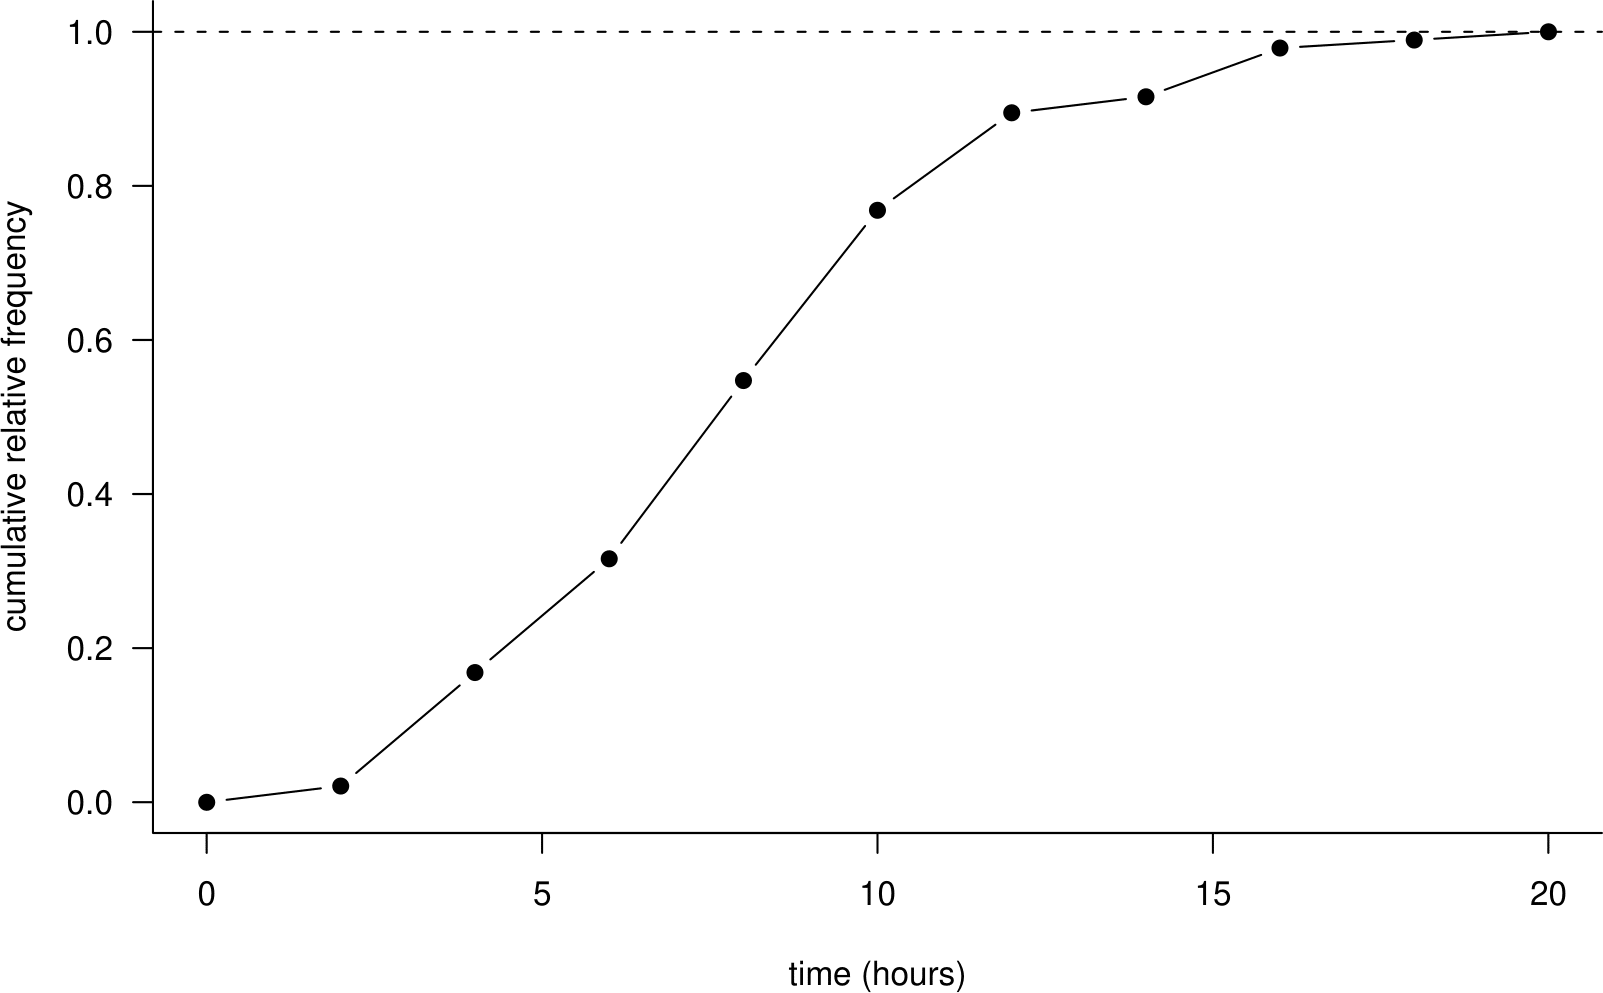
\includegraphics[width=0.75\linewidth]{images/ox_cum_freq} 

}

\caption{A cumulative relative frequency distribution of the Oxford birth times.}\label{fig:oxcumfreq}
\end{figure}

The shape of this plot depends on the choice of the classes. We could increase the detail in the plot by increasing the number of classes, that is, by decreasing the class width. In an extreme case we could choose the classes so that there is a class for every unique value in the data. Table \ref{tab:oxfreqecdf} shows how this could be done.



 
  \providecommand{\huxb}[2]{\arrayrulecolor[RGB]{#1}\global\arrayrulewidth=#2pt}
  \providecommand{\huxvb}[2]{\color[RGB]{#1}\vrule width #2pt}
  \providecommand{\huxtpad}[1]{\rule{0pt}{#1}}
  \providecommand{\huxbpad}[1]{\rule[-#1]{0pt}{#1}}

\begin{table}[ht]
\begin{centerbox}
\begin{threeparttable}
\captionsetup{justification=centering,singlelinecheck=off}
\caption{\label{tab:oxfreqecdf} Frequency table of the Oxford birth times, with one observation per class.}
 \setlength{\tabcolsep}{0pt}
\begin{tabularx}{0.8\textwidth}{p{0.16\textwidth} p{0.16\textwidth} p{0.16\textwidth} p{0.16\textwidth} p{0.16\textwidth}}


\hhline{>{\huxb{0, 0, 0}{1}}->{\huxb{0, 0, 0}{1}}->{\huxb{0, 0, 0}{1}}->{\huxb{0, 0, 0}{1}}->{\huxb{0, 0, 0}{1}}-}
\arrayrulecolor{black}

\multicolumn{1}{!{\huxvb{0, 0, 0}{0}}p{0.16\textwidth}!{\huxvb{0, 0, 0}{0}}}{\cellcolor[RGB]{255, 255, 255}\hspace{6pt}\parbox[b]{0.16\textwidth-6pt-6pt}{\huxtpad{0pt + 1em}\centering time (hours)\huxbpad{0pt}}} &
\multicolumn{1}{p{0.16\textwidth}!{\huxvb{0, 0, 0}{0}}}{\cellcolor[RGB]{255, 255, 255}\hspace{6pt}\parbox[b]{0.16\textwidth-6pt-6pt}{\huxtpad{0pt + 1em}\centering frequency\huxbpad{0pt}}} &
\multicolumn{1}{p{0.16\textwidth}!{\huxvb{0, 0, 0}{0}}}{\cellcolor[RGB]{255, 255, 255}\hspace{6pt}\parbox[b]{0.16\textwidth-6pt-6pt}{\huxtpad{0pt + 1em}\centering relative frequency\huxbpad{0pt}}} &
\multicolumn{1}{p{0.16\textwidth}!{\huxvb{0, 0, 0}{0}}}{\cellcolor[RGB]{255, 255, 255}\hspace{6pt}\parbox[b]{0.16\textwidth-6pt-6pt}{\huxtpad{0pt + 1em}\centering cumulative frequency\huxbpad{0pt}}} &
\multicolumn{1}{p{0.16\textwidth}!{\huxvb{0, 0, 0}{0}}}{\cellcolor[RGB]{255, 255, 255}\hspace{6pt}\parbox[b]{0.16\textwidth-6pt-6pt}{\huxtpad{0pt + 1em}\centering cumulative relative frequency\huxbpad{0pt}}} \tabularnewline[-0.5pt]


\hhline{>{\huxb{0, 0, 0}{1}}->{\huxb{0, 0, 0}{1}}->{\huxb{0, 0, 0}{1}}->{\huxb{0, 0, 0}{1}}->{\huxb{0, 0, 0}{1}}-}
\arrayrulecolor{black}

\multicolumn{1}{!{\huxvb{0, 0, 0}{0}}p{0.16\textwidth}!{\huxvb{0, 0, 0}{0}}}{\cellcolor[RGB]{255, 255, 255}\hspace{6pt}\parbox[b]{0.16\textwidth-6pt-6pt}{\huxtpad{0pt + 1em}\centering 0.0-1.5\huxbpad{0pt}}} &
\multicolumn{1}{p{0.16\textwidth}!{\huxvb{0, 0, 0}{0}}}{\cellcolor[RGB]{255, 255, 255}\hspace{6pt}\parbox[b]{0.16\textwidth-6pt-6pt}{\huxtpad{0pt + 1em}\centering 1\huxbpad{0pt}}} &
\multicolumn{1}{p{0.16\textwidth}!{\huxvb{0, 0, 0}{0}}}{\cellcolor[RGB]{255, 255, 255}\hspace{6pt}\parbox[b]{0.16\textwidth-6pt-6pt}{\huxtpad{0pt + 1em}\centering 1/95\huxbpad{0pt}}} &
\multicolumn{1}{p{0.16\textwidth}!{\huxvb{0, 0, 0}{0}}}{\cellcolor[RGB]{255, 255, 255}\hspace{6pt}\parbox[b]{0.16\textwidth-6pt-6pt}{\huxtpad{0pt + 1em}\centering 1\huxbpad{0pt}}} &
\multicolumn{1}{p{0.16\textwidth}!{\huxvb{0, 0, 0}{0}}}{\cellcolor[RGB]{255, 255, 255}\hspace{6pt}\parbox[b]{0.16\textwidth-6pt-6pt}{\huxtpad{0pt + 1em}\centering 1/95\huxbpad{0pt}}} \tabularnewline[-0.5pt]


\hhline{>{\huxb{255, 255, 255}{0.1}}->{\huxb{255, 255, 255}{0.1}}->{\huxb{255, 255, 255}{0.1}}->{\huxb{255, 255, 255}{0.1}}->{\huxb{255, 255, 255}{0.1}}-}
\arrayrulecolor{black}

\multicolumn{1}{!{\huxvb{0, 0, 0}{0}}p{0.16\textwidth}!{\huxvb{0, 0, 0}{0}}}{\cellcolor[RGB]{255, 255, 255}\hspace{6pt}\parbox[b]{0.16\textwidth-6pt-6pt}{\huxtpad{0pt + 1em}\centering 1.5-2.0\huxbpad{0pt}}} &
\multicolumn{1}{p{0.16\textwidth}!{\huxvb{0, 0, 0}{0}}}{\cellcolor[RGB]{255, 255, 255}\hspace{6pt}\parbox[b]{0.16\textwidth-6pt-6pt}{\huxtpad{0pt + 1em}\centering 1\huxbpad{0pt}}} &
\multicolumn{1}{p{0.16\textwidth}!{\huxvb{0, 0, 0}{0}}}{\cellcolor[RGB]{255, 255, 255}\hspace{6pt}\parbox[b]{0.16\textwidth-6pt-6pt}{\huxtpad{0pt + 1em}\centering 1/95\huxbpad{0pt}}} &
\multicolumn{1}{p{0.16\textwidth}!{\huxvb{0, 0, 0}{0}}}{\cellcolor[RGB]{255, 255, 255}\hspace{6pt}\parbox[b]{0.16\textwidth-6pt-6pt}{\huxtpad{0pt + 1em}\centering 2\huxbpad{0pt}}} &
\multicolumn{1}{p{0.16\textwidth}!{\huxvb{0, 0, 0}{0}}}{\cellcolor[RGB]{255, 255, 255}\hspace{6pt}\parbox[b]{0.16\textwidth-6pt-6pt}{\huxtpad{0pt + 1em}\centering 2/95\huxbpad{0pt}}} \tabularnewline[-0.5pt]


\hhline{>{\huxb{255, 255, 255}{0.1}}->{\huxb{255, 255, 255}{0.1}}->{\huxb{255, 255, 255}{0.1}}->{\huxb{255, 255, 255}{0.1}}->{\huxb{255, 255, 255}{0.1}}-}
\arrayrulecolor{black}

\multicolumn{1}{!{\huxvb{0, 0, 0}{0}}p{0.16\textwidth}!{\huxvb{0, 0, 0}{0}}}{\cellcolor[RGB]{255, 255, 255}\hspace{6pt}\parbox[b]{0.16\textwidth-6pt-6pt}{\huxtpad{0pt + 1em}\centering 2.0-2.1\huxbpad{0pt}}} &
\multicolumn{1}{p{0.16\textwidth}!{\huxvb{0, 0, 0}{0}}}{\cellcolor[RGB]{255, 255, 255}\hspace{6pt}\parbox[b]{0.16\textwidth-6pt-6pt}{\huxtpad{0pt + 1em}\centering 1\huxbpad{0pt}}} &
\multicolumn{1}{p{0.16\textwidth}!{\huxvb{0, 0, 0}{0}}}{\cellcolor[RGB]{255, 255, 255}\hspace{6pt}\parbox[b]{0.16\textwidth-6pt-6pt}{\huxtpad{0pt + 1em}\centering 1/95\huxbpad{0pt}}} &
\multicolumn{1}{p{0.16\textwidth}!{\huxvb{0, 0, 0}{0}}}{\cellcolor[RGB]{255, 255, 255}\hspace{6pt}\parbox[b]{0.16\textwidth-6pt-6pt}{\huxtpad{0pt + 1em}\centering 3\huxbpad{0pt}}} &
\multicolumn{1}{p{0.16\textwidth}!{\huxvb{0, 0, 0}{0}}}{\cellcolor[RGB]{255, 255, 255}\hspace{6pt}\parbox[b]{0.16\textwidth-6pt-6pt}{\huxtpad{0pt + 1em}\centering 3/95\huxbpad{0pt}}} \tabularnewline[-0.5pt]


\hhline{>{\huxb{255, 255, 255}{0.1}}->{\huxb{255, 255, 255}{0.1}}->{\huxb{255, 255, 255}{0.1}}->{\huxb{255, 255, 255}{0.1}}->{\huxb{255, 255, 255}{0.1}}-}
\arrayrulecolor{black}

\multicolumn{1}{!{\huxvb{0, 0, 0}{0}}p{0.16\textwidth}!{\huxvb{0, 0, 0}{0}}}{\cellcolor[RGB]{255, 255, 255}\hspace{6pt}\parbox[b]{0.16\textwidth-6pt-6pt}{\huxtpad{0pt + 1em}\centering 2.1-2.5\huxbpad{0pt}}} &
\multicolumn{1}{p{0.16\textwidth}!{\huxvb{0, 0, 0}{0}}}{\cellcolor[RGB]{255, 255, 255}\hspace{6pt}\parbox[b]{0.16\textwidth-6pt-6pt}{\huxtpad{0pt + 1em}\centering 2\huxbpad{0pt}}} &
\multicolumn{1}{p{0.16\textwidth}!{\huxvb{0, 0, 0}{0}}}{\cellcolor[RGB]{255, 255, 255}\hspace{6pt}\parbox[b]{0.16\textwidth-6pt-6pt}{\huxtpad{0pt + 1em}\centering 2/95\huxbpad{0pt}}} &
\multicolumn{1}{p{0.16\textwidth}!{\huxvb{0, 0, 0}{0}}}{\cellcolor[RGB]{255, 255, 255}\hspace{6pt}\parbox[b]{0.16\textwidth-6pt-6pt}{\huxtpad{0pt + 1em}\centering 5\huxbpad{0pt}}} &
\multicolumn{1}{p{0.16\textwidth}!{\huxvb{0, 0, 0}{0}}}{\cellcolor[RGB]{255, 255, 255}\hspace{6pt}\parbox[b]{0.16\textwidth-6pt-6pt}{\huxtpad{0pt + 1em}\centering 5/95\huxbpad{0pt}}} \tabularnewline[-0.5pt]


\hhline{>{\huxb{255, 255, 255}{0.1}}->{\huxb{255, 255, 255}{0.1}}->{\huxb{255, 255, 255}{0.1}}->{\huxb{255, 255, 255}{0.1}}->{\huxb{255, 255, 255}{0.1}}-}
\arrayrulecolor{black}

\multicolumn{1}{!{\huxvb{0, 0, 0}{0}}p{0.16\textwidth}!{\huxvb{0, 0, 0}{0}}}{\cellcolor[RGB]{255, 255, 255}\hspace{6pt}\parbox[b]{0.16\textwidth-6pt-6pt}{\huxtpad{0pt + 1em}\centering ...\huxbpad{0pt}}} &
\multicolumn{1}{p{0.16\textwidth}!{\huxvb{0, 0, 0}{0}}}{\cellcolor[RGB]{255, 255, 255}\hspace{6pt}\parbox[b]{0.16\textwidth-6pt-6pt}{\huxtpad{0pt + 1em}\centering ...\huxbpad{0pt}}} &
\multicolumn{1}{p{0.16\textwidth}!{\huxvb{0, 0, 0}{0}}}{\cellcolor[RGB]{255, 255, 255}\hspace{6pt}\parbox[b]{0.16\textwidth-6pt-6pt}{\huxtpad{0pt + 1em}\centering ...\huxbpad{0pt}}} &
\multicolumn{1}{p{0.16\textwidth}!{\huxvb{0, 0, 0}{0}}}{\cellcolor[RGB]{255, 255, 255}\hspace{6pt}\parbox[b]{0.16\textwidth-6pt-6pt}{\huxtpad{0pt + 1em}\centering ...\huxbpad{0pt}}} &
\multicolumn{1}{p{0.16\textwidth}!{\huxvb{0, 0, 0}{0}}}{\cellcolor[RGB]{255, 255, 255}\hspace{6pt}\parbox[b]{0.16\textwidth-6pt-6pt}{\huxtpad{0pt + 1em}\centering ...\huxbpad{0pt}}} \tabularnewline[-0.5pt]


\hhline{>{\huxb{255, 255, 255}{0.1}}->{\huxb{255, 255, 255}{0.1}}->{\huxb{255, 255, 255}{0.1}}->{\huxb{255, 255, 255}{0.1}}->{\huxb{255, 255, 255}{0.1}}-}
\arrayrulecolor{black}

\multicolumn{1}{!{\huxvb{0, 0, 0}{0}}p{0.16\textwidth}!{\huxvb{0, 0, 0}{0}}}{\cellcolor[RGB]{255, 255, 255}\hspace{6pt}\parbox[b]{0.16\textwidth-6pt-6pt}{\huxtpad{0pt + 1em}\centering 16.0-16.5\huxbpad{0pt}}} &
\multicolumn{1}{p{0.16\textwidth}!{\huxvb{0, 0, 0}{0}}}{\cellcolor[RGB]{255, 255, 255}\hspace{6pt}\parbox[b]{0.16\textwidth-6pt-6pt}{\huxtpad{0pt + 1em}\centering 1\huxbpad{0pt}}} &
\multicolumn{1}{p{0.16\textwidth}!{\huxvb{0, 0, 0}{0}}}{\cellcolor[RGB]{255, 255, 255}\hspace{6pt}\parbox[b]{0.16\textwidth-6pt-6pt}{\huxtpad{0pt + 1em}\centering 1/95\huxbpad{0pt}}} &
\multicolumn{1}{p{0.16\textwidth}!{\huxvb{0, 0, 0}{0}}}{\cellcolor[RGB]{255, 255, 255}\hspace{6pt}\parbox[b]{0.16\textwidth-6pt-6pt}{\huxtpad{0pt + 1em}\centering 94\huxbpad{0pt}}} &
\multicolumn{1}{p{0.16\textwidth}!{\huxvb{0, 0, 0}{0}}}{\cellcolor[RGB]{255, 255, 255}\hspace{6pt}\parbox[b]{0.16\textwidth-6pt-6pt}{\huxtpad{0pt + 1em}\centering 94/95\huxbpad{0pt}}} \tabularnewline[-0.5pt]


\hhline{>{\huxb{255, 255, 255}{0.1}}->{\huxb{255, 255, 255}{0.1}}->{\huxb{255, 255, 255}{0.1}}->{\huxb{255, 255, 255}{0.1}}->{\huxb{255, 255, 255}{0.1}}-}
\arrayrulecolor{black}

\multicolumn{1}{!{\huxvb{0, 0, 0}{0}}p{0.16\textwidth}!{\huxvb{0, 0, 0}{0}}}{\cellcolor[RGB]{255, 255, 255}\hspace{6pt}\parbox[b]{0.16\textwidth-6pt-6pt}{\huxtpad{0pt + 1em}\centering 16.5-19.0\huxbpad{0pt}}} &
\multicolumn{1}{p{0.16\textwidth}!{\huxvb{0, 0, 0}{0}}}{\cellcolor[RGB]{255, 255, 255}\hspace{6pt}\parbox[b]{0.16\textwidth-6pt-6pt}{\huxtpad{0pt + 1em}\centering 1\huxbpad{0pt}}} &
\multicolumn{1}{p{0.16\textwidth}!{\huxvb{0, 0, 0}{0}}}{\cellcolor[RGB]{255, 255, 255}\hspace{6pt}\parbox[b]{0.16\textwidth-6pt-6pt}{\huxtpad{0pt + 1em}\centering 1/95\huxbpad{0pt}}} &
\multicolumn{1}{p{0.16\textwidth}!{\huxvb{0, 0, 0}{0}}}{\cellcolor[RGB]{255, 255, 255}\hspace{6pt}\parbox[b]{0.16\textwidth-6pt-6pt}{\huxtpad{0pt + 1em}\centering 95\huxbpad{0pt}}} &
\multicolumn{1}{p{0.16\textwidth}!{\huxvb{0, 0, 0}{0}}}{\cellcolor[RGB]{255, 255, 255}\hspace{6pt}\parbox[b]{0.16\textwidth-6pt-6pt}{\huxtpad{0pt + 1em}\centering 1\huxbpad{0pt}}} \tabularnewline[-0.5pt]


\hhline{>{\huxb{0, 0, 0}{1}}->{\huxb{0, 0, 0}{1}}->{\huxb{0, 0, 0}{1}}->{\huxb{0, 0, 0}{1}}->{\huxb{0, 0, 0}{1}}-}
\arrayrulecolor{black}

\multicolumn{1}{!{\huxvb{0, 0, 0}{0}}p{0.16\textwidth}!{\huxvb{0, 0, 0}{0}}}{\cellcolor[RGB]{255, 255, 255}\hspace{6pt}\parbox[b]{0.16\textwidth-6pt-6pt}{\huxtpad{0pt + 1em}\centering total\huxbpad{0pt}}} &
\multicolumn{1}{p{0.16\textwidth}!{\huxvb{0, 0, 0}{0}}}{\cellcolor[RGB]{255, 255, 255}\hspace{6pt}\parbox[b]{0.16\textwidth-6pt-6pt}{\huxtpad{0pt + 1em}\centering 95\huxbpad{0pt}}} &
\multicolumn{1}{p{0.16\textwidth}!{\huxvb{0, 0, 0}{0}}}{\cellcolor[RGB]{255, 255, 255}\hspace{6pt}\parbox[b]{0.16\textwidth-6pt-6pt}{\huxtpad{0pt + 1em}\centering 1\huxbpad{0pt}}} &
\multicolumn{1}{p{0.16\textwidth}!{\huxvb{0, 0, 0}{0}}}{\cellcolor[RGB]{255, 255, 255}\hspace{6pt}\parbox[b]{0.16\textwidth-6pt-6pt}{\huxtpad{0pt + 1em}\centering \huxbpad{0pt}}} &
\multicolumn{1}{p{0.16\textwidth}!{\huxvb{0, 0, 0}{0}}}{\cellcolor[RGB]{255, 255, 255}\hspace{6pt}\parbox[b]{0.16\textwidth-6pt-6pt}{\huxtpad{0pt + 1em}\centering \huxbpad{0pt}}} \tabularnewline[-0.5pt]


\hhline{}
\arrayrulecolor{black}
\end{tabularx}
\end{threeparttable}\par\end{centerbox}

\end{table}
 

Figure \ref{fig:oxcumfreq2} shows the resulting graph. Notice that the shape is similar to Figure \ref{fig:oxcumfreq} but it is less smooth. The function (from time on the horizontal axis to cumulative relative frequency on the vertical axis) is often called the \textbf{empirical cumulative distribution function} or \textbf{empirical c.d.f}. The meaning will become clearer when we look at c.d.f.s in Section \ref{discrete}.

\begin{figure}

{\centering 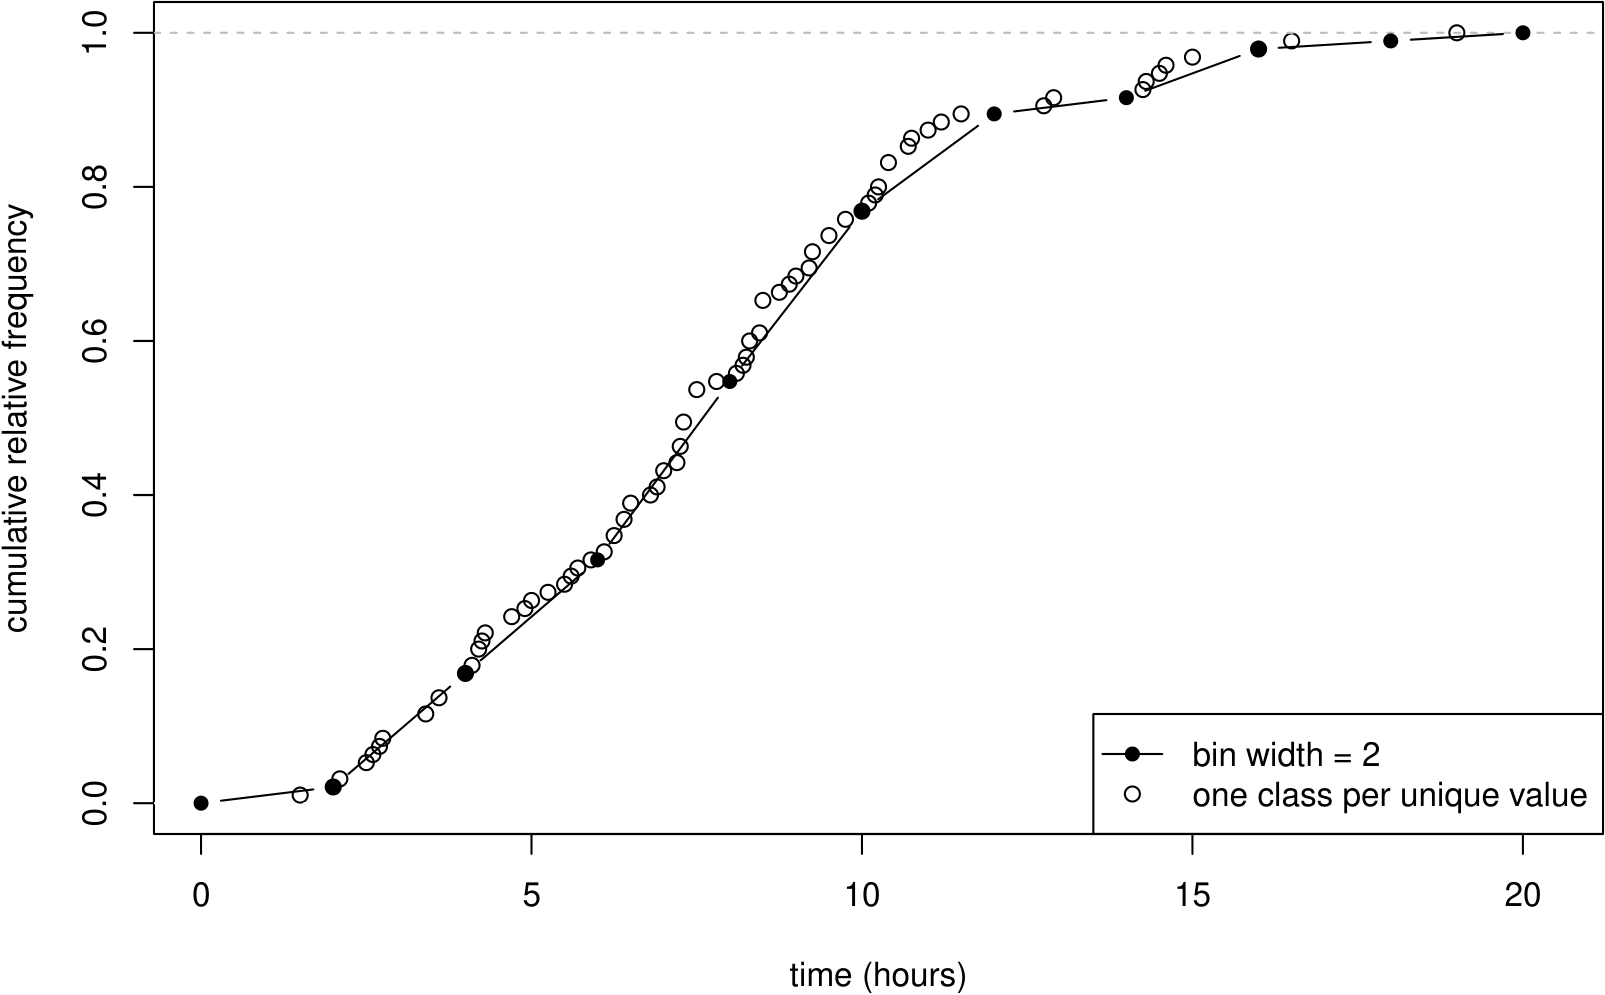
\includegraphics[width=0.75\linewidth]{images/ox_cum_freq2new} 

}

\caption{A cumulative relative frequency distribution of the Oxford birth times, with classes defined so that there is one data value in each class.}\label{fig:oxcumfreq2}
\end{figure}

Sometimes data are given to us in the form of Table \ref{tab:oxfreq} and the individual data values are not available. For example, some birth data published by the Office of National Statistics data give mother's age in 5 year age bands. Data provided in this form are called \textbf{grouped data}. We will analyse data from tables in Chapter \ref{contingency}.

\hypertarget{graphs}{%
\section{Graphs (1 variable)}\label{graphs}}

These days it is very easy to plot a graph using a computer. However, \textbf{you} need to decide which type of graph is appropriate and the default graph produced by the computer may not be very good. Some general rules:

\begin{itemize}
\tightlist
\item
  \textbf{Always plot the data}. Often this will show clearly the important features of the data. Formal statistical methods may be unnecessary or simply confirm the visual impression given by the plot. Also, plotting the data can reveal potential problems with the data, for example, outlying observations which do not fit in the with the general pattern of the data, or data which are clearly wrong.
\item
  For datasets with more than one variable always plot the variables against
  each other. There may be observations which are not unusual when variables are considered separately but are clearly unusual when 2 variables are plotted. See Section \ref{graphs2}.
\item
  A good graph draws attention to important aspects of the data. Anything which distracts the viewer, for example, excessive shading, symbols, 3-dimensional effects, should be removed.\\
\item
  Axis labels (remember the units!), the legend and caption should enable the viewer of the graph to understand the content of the graph.
\end{itemize}

\hypertarget{histogram}{%
\subsection{Histograms}\label{histogram}}

A \textbf{histogram} is a graphical display based on the relative frequency distribution of a set of data on a \textbf{continuous} variable. The variable of interest is plotted on the \(x\)-axis, which is divided into \textbf{bins} based on the classes of the frequency distribution. A rectangle is plotted for each bin. The height of a rectangle is calculated as
\begin{equation}
\mbox{height} = \frac{\mbox{relative frequency}}{\mbox{bin width}} = \frac{\mbox{frequency}}{n \times \mbox{bin width}}.
\label{eq:hist}
\end{equation}
Therefore, for a given box in the histogram:

\begin{itemize}
\tightlist
\item
  the \textbf{area} represents the relative frequency of the observations in
  the interval;
\item
  the \textbf{height} represents the relative frequency of the observations in
  the interval \textbf{per unit of measurement}, commonly known as the \textbf{density}.
\end{itemize}

The total area under a histogram is equal to 1. In fact a histogram is an estimate of a probability density function (see Section \ref{continuous}). The vertical axis is commonly labelled \textbf{density}.

It is common for people to plot frequencies (rather than relative frequencies per unit), giving what I will call a \textbf{frequency plot}, that is, \textbf{not} a true histogram.

If the bin widths are equal the shape of frequency plot is the same as the corresponding histogram. However, when drawing a frequency plot using unequal bin widths it is important to take into account the differing widths of the bins. For example, in the plot on the bottom left of Figure \ref{fig:oxhistbasic}, the frequency in the box for 12-20 hours is 4 times too high because the longer width of this interval has not been taken into account.
One solution is to divide the frequencies by the bin width to produce frequencies \textbf{per unit}, but then we may as well produce a true histogram, using equation \eqref{eq:hist}.

\begin{figure}

{\centering 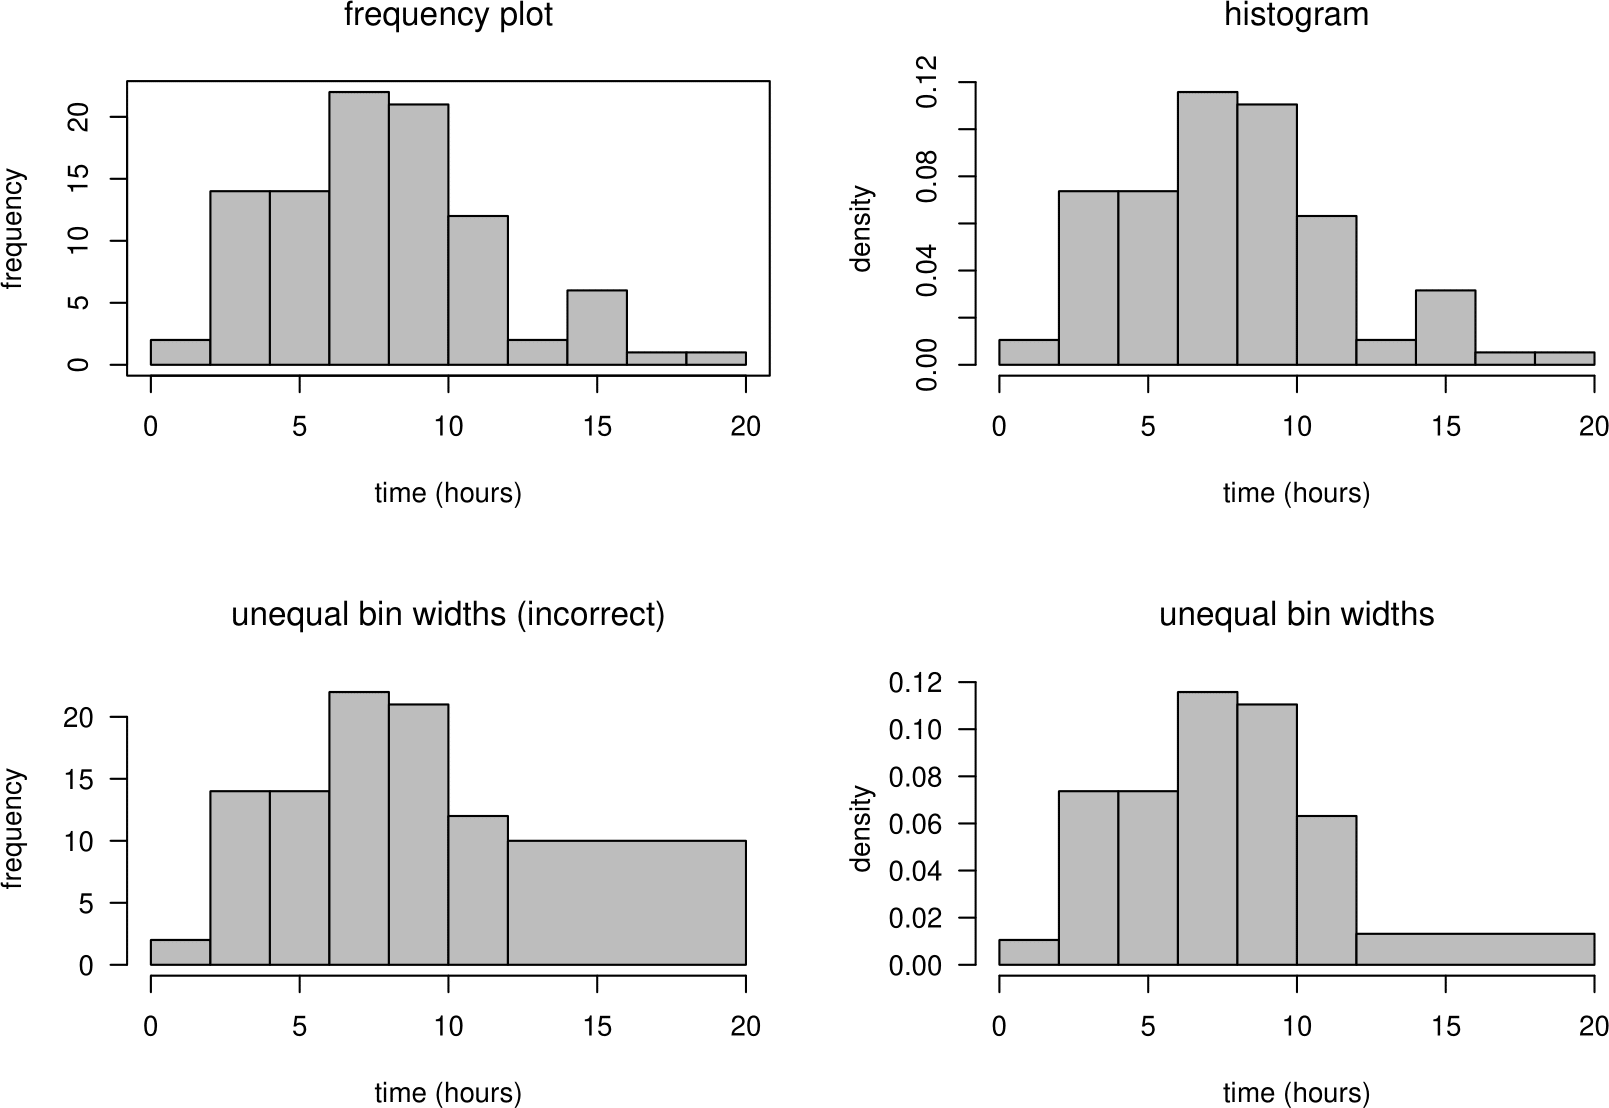
\includegraphics[width=0.75\linewidth]{images/ox_hist_basic} 

}

\caption{Frequency plots (left) and histograms (right) of the Oxford birth times.}\label{fig:oxhistbasic}
\end{figure}

A histogram can be useful to look at the shape of a distribution. However,
especially for a small dataset, the shape of the histogram can depend greatly on the classes chosen to define the bins. Figure \ref{fig:oxhistbasic} contains histograms and frequency histograms of the all the times in Table \ref{tab:taboxbirths}. From the histograms we can easily see that the birth times data are slightly positively skewed.

\hypertarget{stem}{%
\subsection{Stem-and-leaf plots}\label{stem}}

A \textbf{stem-and-leaf plot} (or stem plot) is like an enhanced histogram. The \textbf{stem}, on the left, contain the times in whole hours. The \textbf{leaves},
on the right, contain the first digit after the decimal point. An advantage of a stem-and-leaf plot is that it gives the entire dataset (perhaps rounded) in sorted order. It is easy to calculate the five number summary of the data from a stem-and-leaf plot. Figure \ref{fig:oxstem} shows a stem-and-leaf plot of the Oxford births data.

\begin{figure}

{\centering 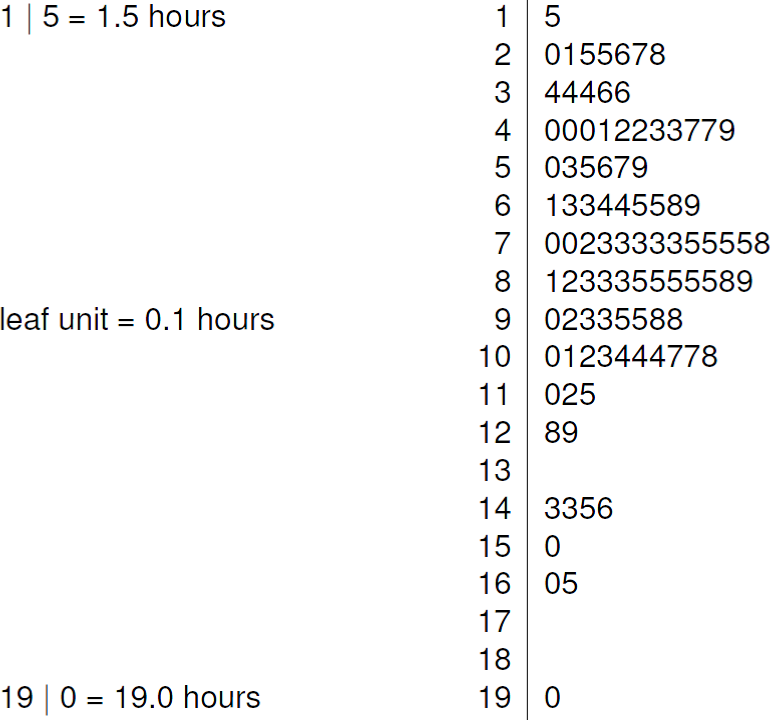
\includegraphics[width=0.6\linewidth]{images/ox_stem} 

}

\caption{Stem-and-leaf plot of the Oxford birth times. The decimal point is at the vertical line |. The data are rounded to the nearest 0.1 before plotting.}\label{fig:oxstem}
\end{figure}

\hypertarget{dotplots}{%
\subsection{Dotplots}\label{dotplots}}

Dotplots are simple plots in which each observation is represented by a dot. If there are repeated observations, that is, observations with the same value (perhaps after rounding), then their dots are stacked on top of each other. Figure \ref{fig:oxdotbasic} shows two dotplots. In the right hand plot the data were rounded to the nearest hour, producing a plot that looks a bit like a histogram with a bin width of 1 hour, with rectangles replaced by vertical lines of dots.

\begin{figure}

{\centering 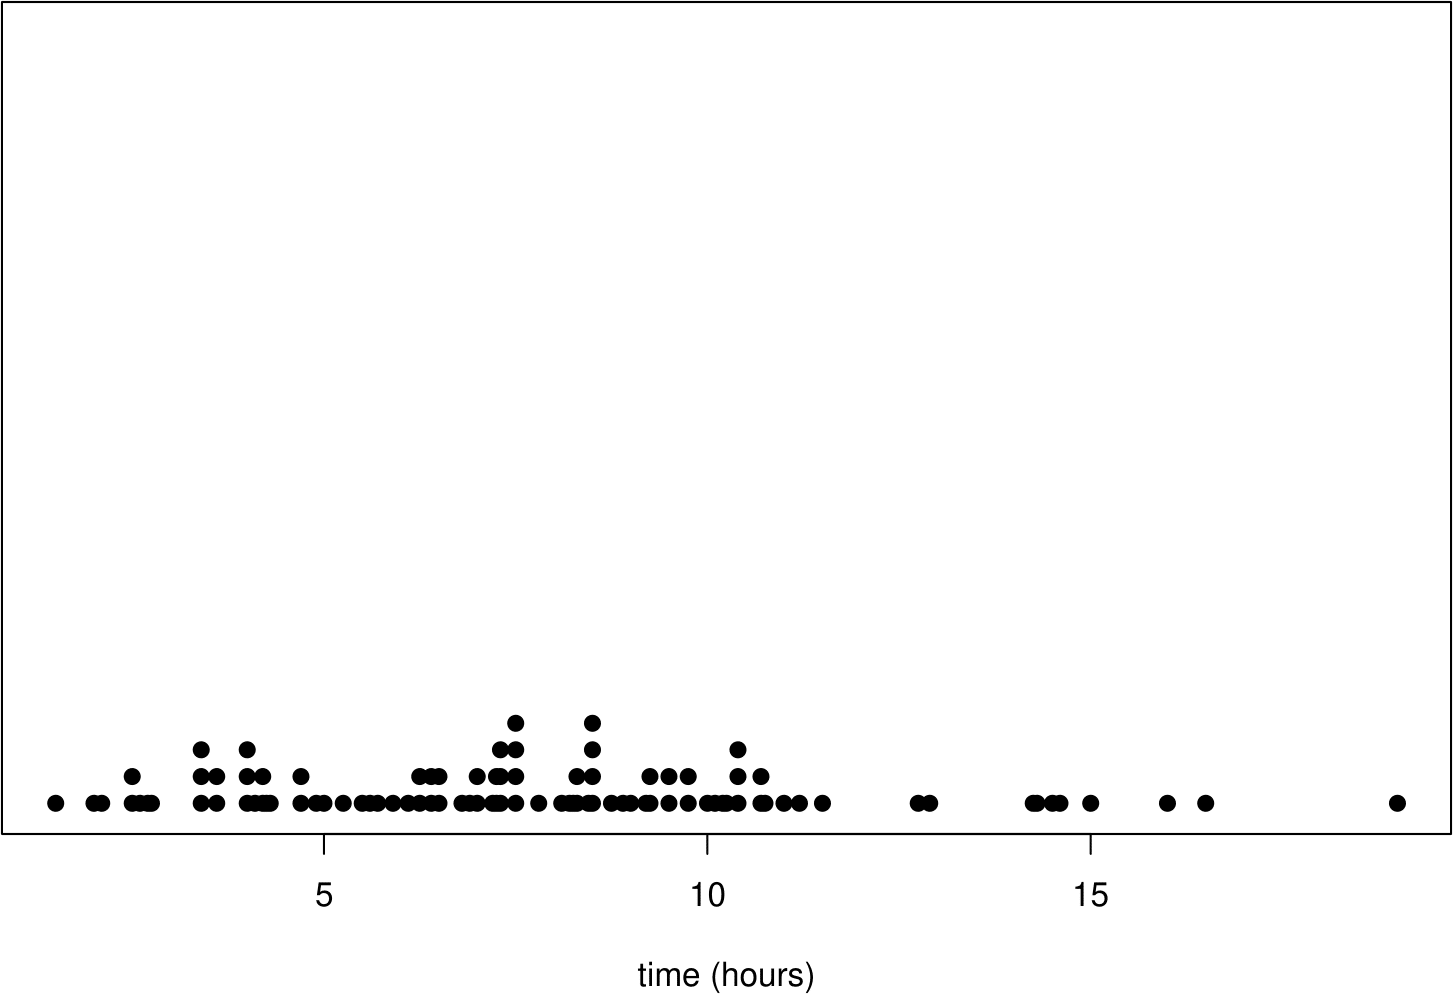
\includegraphics[width=0.75\linewidth]{images/ox_dot_basic} 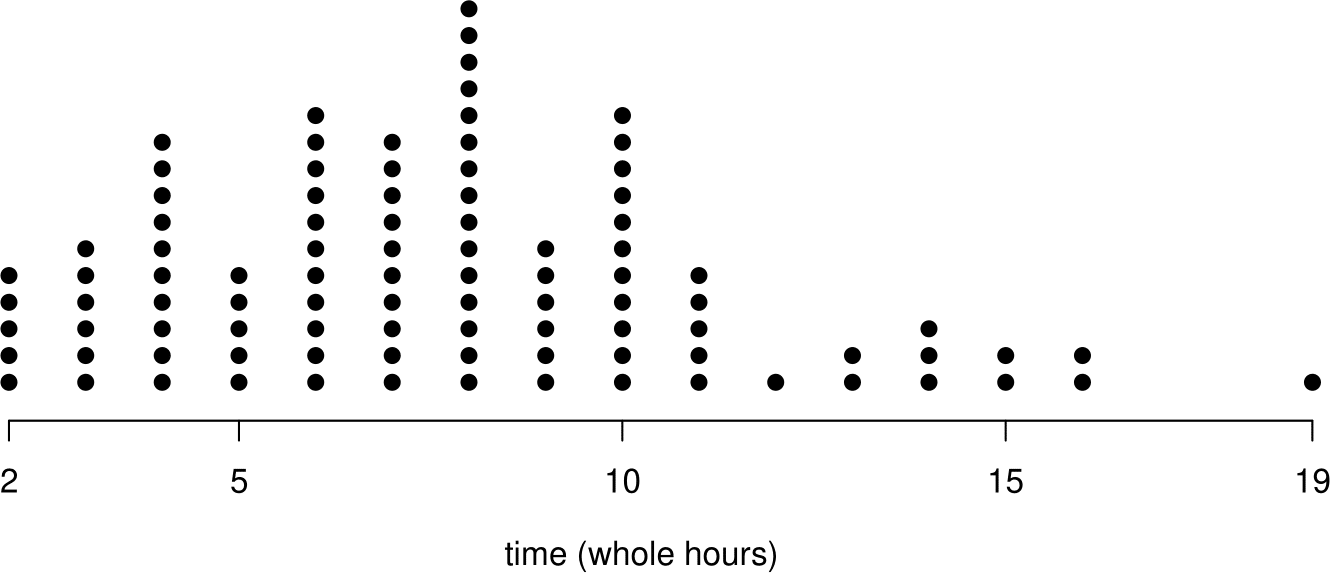
\includegraphics[width=0.75\linewidth]{images/ox_dot_adv} 

}

\caption{Dotplots of the Oxford birth times. Top: raw data (and lots of wasted white space).  Bottom: data rounded to the nearest hour.}\label{fig:oxdotbasic}
\end{figure}

\hypertarget{boxplots}{%
\subsection{Boxplots}\label{boxplots}}

A \textbf{boxplot} (or box-and-whisker plot) is a graphical display containing the five-number summary. It also provides ways to assess the overall shape of the data. Figure \ref{fig:oxdotbasic} explains how a standard boxplot is constructed.

\begin{figure}

{\centering 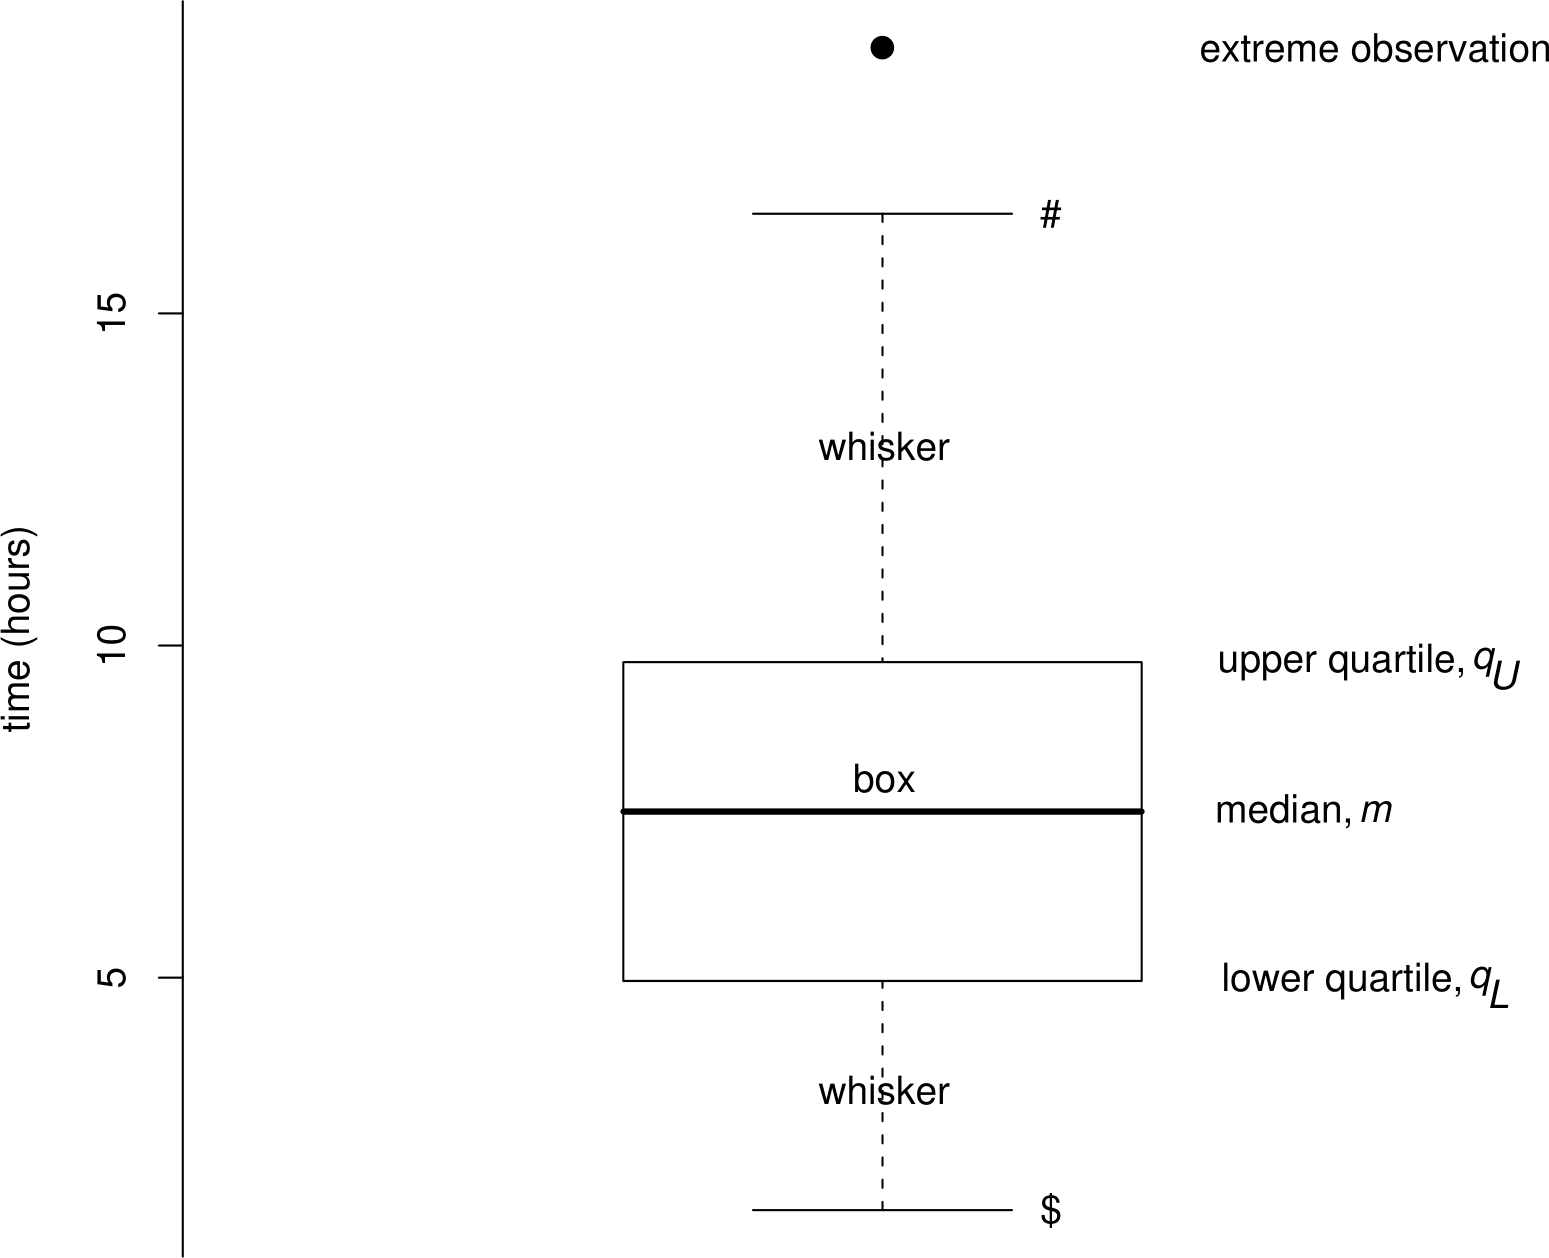
\includegraphics[width=0.75\linewidth]{images/ox_box_basic} 

}

\caption{Boxplot of the Oxford birth times. The upper end (\#) of the upper whisker is drawn at the largest observation within a distance $1.5 (q_U-q_L)$ of $q_U$. The lower end (\$) of the lower whisker is drawn at the smallest observation within a distance $1.5 (q_U-q_L)$ of $q_L$.}\label{fig:oxboxbasic}
\end{figure}

The `box' shows where 50\% of the data lie, that is, between the lower and uper
quartiles. The `whiskers' extend to the most extreme observations that are within 1.5 IQR of the ends of the box. Sometimes a different criterion is used to determine the ends of the whiskers. Any more extreme values are individually identified (with a dot here).

It can less easy easy to come to a conclusion concerning the nature of skewness using a boxplot than using a histogram. In this example the lengths of the whiskers and the presence of the value at 19 hours suggest slight positive skewness. However, the relative positions of the samples quartiles suggest (very slight) negative skewness, which is the cause of the slightly negative value of sample quartiles skewness towards the end of Section \ref{symmetry}.

Some alternatives are given in Figure \ref{fig:oxboxadv}. Which do you prefer?

\begin{figure}

{\centering 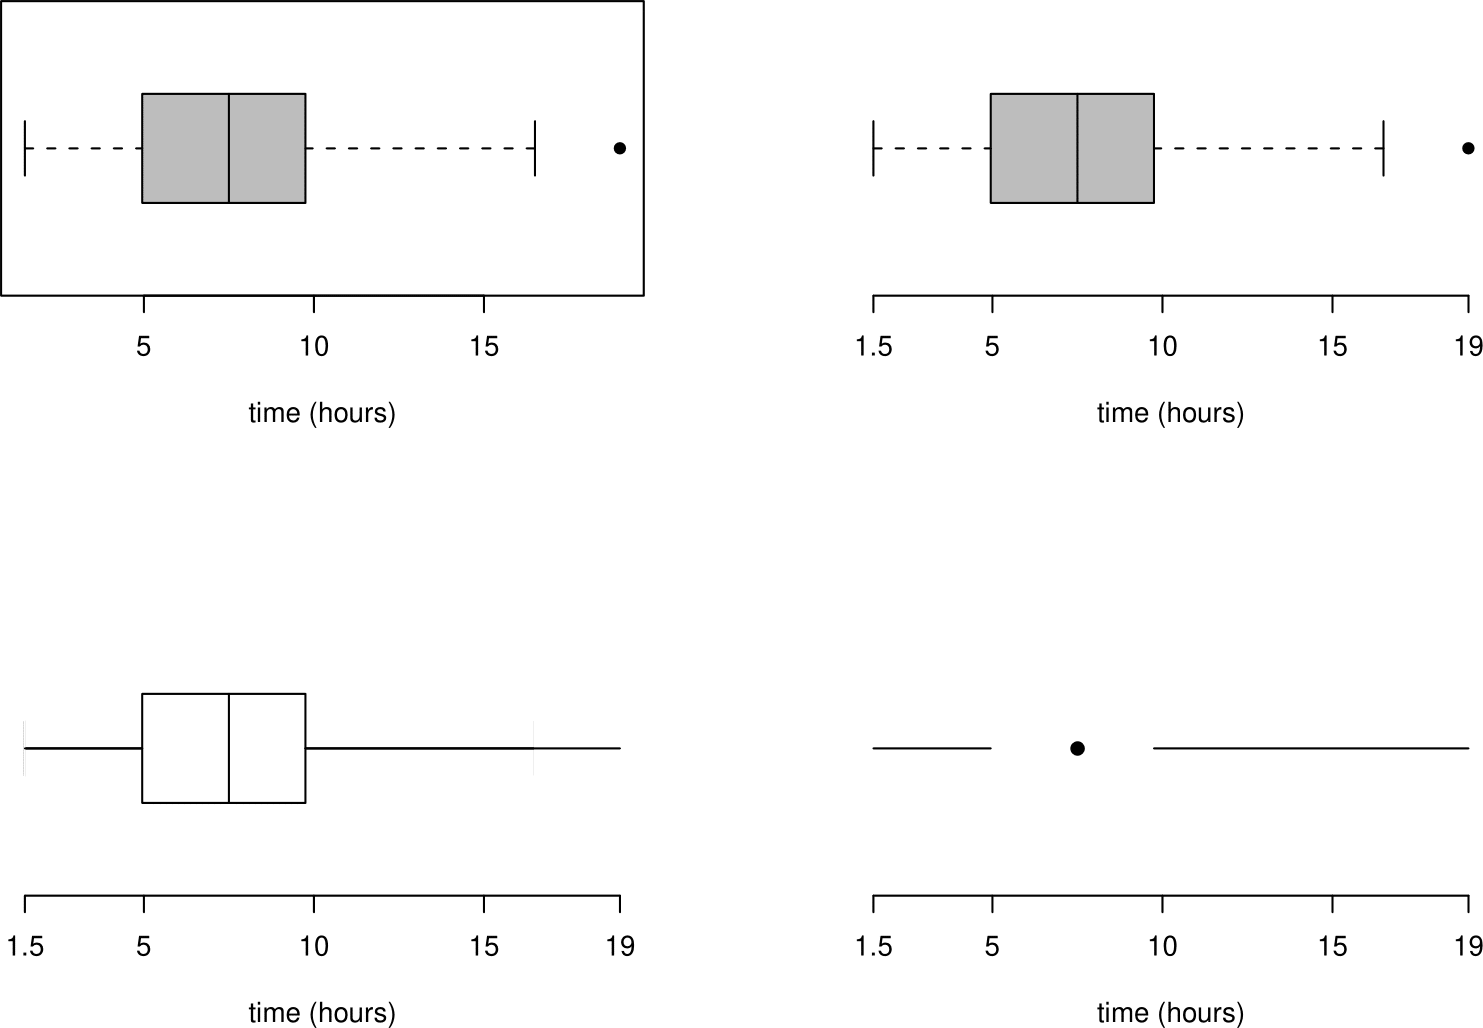
\includegraphics[width=0.75\linewidth]{images/ox_box_adv} 

}

\caption{Alternative plots of the Oxford birth times based on the five-figure summary.}\label{fig:oxboxadv}
\end{figure}

\hypertarget{barplots}{%
\subsection{Barplots}\label{barplots}}

A \textbf{barplot} (or bar chart) has a similar appearance to a histogram but is used for numerical discrete data or categorical data. Therefore there are gaps between the bars in a barplot.

\hypertarget{example-numerical-discrete-data}{%
\subsubsection*{Example: numerical discrete data}\label{example-numerical-discrete-data}}
\addcontentsline{toc}{subsubsection}{Example: numerical discrete data}

Table \ref{tab:shuttlenew} shows the frequencies of the number of damaged O-rings in the space shuttle example. Figure \ref{fig:shuttlebarplots} shows barplots (or equivalent) of these data. Which do you prefer?

\begin{table}

\caption{\label{tab:shuttlenew}Frequencies of numbers of damaged O-rings for the space shuttle data.}
\centering
\begin{tabular}[t]{lllll}
\toprule
number of damaged O-rings & 0 & 1 & 2 & 3\\
frequency & 16 & 5 & 1 & 1\\
\bottomrule
\end{tabular}
\end{table}

\begin{figure}

{\centering 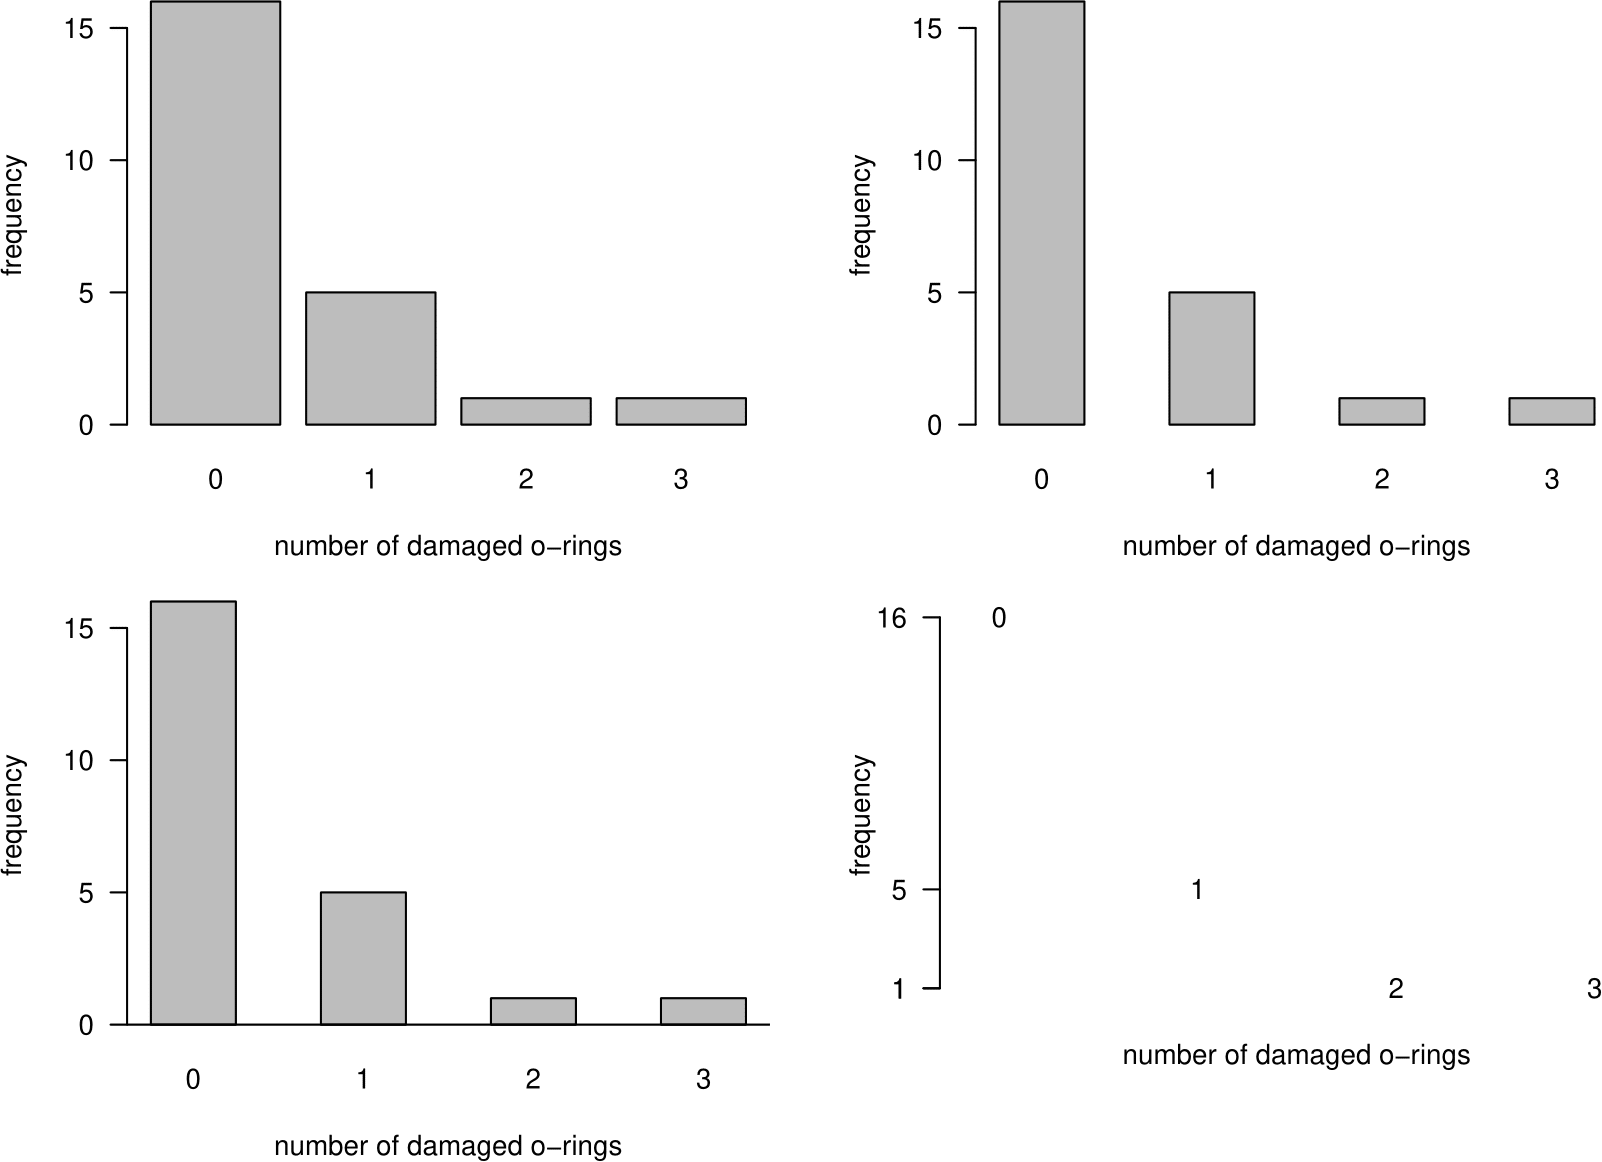
\includegraphics[width=0.75\linewidth]{images/shuttle_barplots} 

}

\caption{Barplots of numbers of damaged O-rings on space shuttle flights.}\label{fig:shuttlebarplots}
\end{figure}

\hypertarget{example-categorical-data}{%
\subsubsection*{Example: categorical data}\label{example-categorical-data}}
\addcontentsline{toc}{subsubsection}{Example: categorical data}

Table \ref{tab:ABOnew} shows the percentages of people in the UK with the 8 main blood groups O\(+\), A\(+\), B\(+\), AB\(+\), O\(-\), A\(-\), B\(-\) and AB\(-\). See section \ref{bloodindep} for more details about blood groups. These data are nominal.

 
  \providecommand{\huxb}[2]{\arrayrulecolor[RGB]{#1}\global\arrayrulewidth=#2pt}
  \providecommand{\huxvb}[2]{\color[RGB]{#1}\vrule width #2pt}
  \providecommand{\huxtpad}[1]{\rule{0pt}{#1}}
  \providecommand{\huxbpad}[1]{\rule[-#1]{0pt}{#1}}

\begin{table}[ht]
\begin{centerbox}
\begin{threeparttable}
\captionsetup{justification=centering,singlelinecheck=off}
\caption{\label{tab:ABOnew} Percentages of people in the UK with the 8 main blood groups}
 \setlength{\tabcolsep}{0pt}
\begin{tabularx}{0.8\textwidth}{p{0.2\textwidth} p{0.2\textwidth} p{0.2\textwidth} p{0.2\textwidth}}


\hhline{>{\huxb{255, 255, 255}{0.1}}->{\huxb{255, 255, 255}{0.1}}->{\huxb{255, 255, 255}{0.1}}->{\huxb{255, 255, 255}{0.1}}-}
\arrayrulecolor{black}

\multicolumn{1}{!{\huxvb{0, 0, 0}{0}}p{0.2\textwidth}!{\huxvb{0, 0, 0}{1}}}{\cellcolor[RGB]{255, 255, 255}\hspace{6pt}\parbox[b]{0.2\textwidth-6pt-6pt}{\huxtpad{6pt + 1em}\centering blood type\huxbpad{6pt}}} &
\multicolumn{1}{p{0.2\textwidth}!{\huxvb{0, 0, 0}{0}}}{\cellcolor[RGB]{255, 255, 255}\hspace{6pt}\parbox[b]{0.2\textwidth-6pt-6pt}{\huxtpad{6pt + 1em}\centering Rh+\huxbpad{6pt}}} &
\multicolumn{1}{p{0.2\textwidth}!{\huxvb{0, 0, 0}{1}}}{\cellcolor[RGB]{255, 255, 255}\hspace{6pt}\parbox[b]{0.2\textwidth-6pt-6pt}{\huxtpad{6pt + 1em}\centering Rh-\huxbpad{6pt}}} &
\multicolumn{1}{p{0.2\textwidth}!{\huxvb{0, 0, 0}{0}}}{\cellcolor[RGB]{255, 255, 255}\hspace{6pt}\parbox[b]{0.2\textwidth-6pt-6pt}{\huxtpad{6pt + 1em}\centering total\huxbpad{6pt}}} \tabularnewline[-0.5pt]


\hhline{>{\huxb{0, 0, 0}{1}}->{\huxb{0, 0, 0}{1}}->{\huxb{0, 0, 0}{1}}->{\huxb{0, 0, 0}{1}}-}
\arrayrulecolor{black}

\multicolumn{1}{!{\huxvb{0, 0, 0}{0}}p{0.2\textwidth}!{\huxvb{0, 0, 0}{1}}}{\cellcolor[RGB]{255, 255, 255}\hspace{6pt}\parbox[b]{0.2\textwidth-6pt-6pt}{\huxtpad{6pt + 1em}\centering O\huxbpad{6pt}}} &
\multicolumn{1}{p{0.2\textwidth}!{\huxvb{0, 0, 0}{0}}}{\cellcolor[RGB]{255, 255, 255}\hspace{6pt}\parbox[b]{0.2\textwidth-6pt-6pt}{\huxtpad{6pt + 1em}\centering 37\huxbpad{6pt}}} &
\multicolumn{1}{p{0.2\textwidth}!{\huxvb{0, 0, 0}{1}}}{\cellcolor[RGB]{255, 255, 255}\hspace{6pt}\parbox[b]{0.2\textwidth-6pt-6pt}{\huxtpad{6pt + 1em}\centering 7\huxbpad{6pt}}} &
\multicolumn{1}{p{0.2\textwidth}!{\huxvb{0, 0, 0}{0}}}{\cellcolor[RGB]{255, 255, 255}\hspace{6pt}\parbox[b]{0.2\textwidth-6pt-6pt}{\huxtpad{6pt + 1em}\centering 44\huxbpad{6pt}}} \tabularnewline[-0.5pt]


\hhline{>{\huxb{255, 255, 255}{0.1}}->{\huxb{255, 255, 255}{0.1}}->{\huxb{255, 255, 255}{0.1}}->{\huxb{255, 255, 255}{0.1}}-}
\arrayrulecolor{black}

\multicolumn{1}{!{\huxvb{0, 0, 0}{0}}p{0.2\textwidth}!{\huxvb{0, 0, 0}{1}}}{\cellcolor[RGB]{255, 255, 255}\hspace{6pt}\parbox[b]{0.2\textwidth-6pt-6pt}{\huxtpad{6pt + 1em}\centering A\huxbpad{6pt}}} &
\multicolumn{1}{p{0.2\textwidth}!{\huxvb{0, 0, 0}{0}}}{\cellcolor[RGB]{255, 255, 255}\hspace{6pt}\parbox[b]{0.2\textwidth-6pt-6pt}{\huxtpad{6pt + 1em}\centering 35\huxbpad{6pt}}} &
\multicolumn{1}{p{0.2\textwidth}!{\huxvb{0, 0, 0}{1}}}{\cellcolor[RGB]{255, 255, 255}\hspace{6pt}\parbox[b]{0.2\textwidth-6pt-6pt}{\huxtpad{6pt + 1em}\centering 7\huxbpad{6pt}}} &
\multicolumn{1}{p{0.2\textwidth}!{\huxvb{0, 0, 0}{0}}}{\cellcolor[RGB]{255, 255, 255}\hspace{6pt}\parbox[b]{0.2\textwidth-6pt-6pt}{\huxtpad{6pt + 1em}\centering 42\huxbpad{6pt}}} \tabularnewline[-0.5pt]


\hhline{>{\huxb{255, 255, 255}{0.1}}->{\huxb{255, 255, 255}{0.1}}->{\huxb{255, 255, 255}{0.1}}->{\huxb{255, 255, 255}{0.1}}-}
\arrayrulecolor{black}

\multicolumn{1}{!{\huxvb{0, 0, 0}{0}}p{0.2\textwidth}!{\huxvb{0, 0, 0}{1}}}{\cellcolor[RGB]{255, 255, 255}\hspace{6pt}\parbox[b]{0.2\textwidth-6pt-6pt}{\huxtpad{6pt + 1em}\centering B\huxbpad{6pt}}} &
\multicolumn{1}{p{0.2\textwidth}!{\huxvb{0, 0, 0}{0}}}{\cellcolor[RGB]{255, 255, 255}\hspace{6pt}\parbox[b]{0.2\textwidth-6pt-6pt}{\huxtpad{6pt + 1em}\centering 8\huxbpad{6pt}}} &
\multicolumn{1}{p{0.2\textwidth}!{\huxvb{0, 0, 0}{1}}}{\cellcolor[RGB]{255, 255, 255}\hspace{6pt}\parbox[b]{0.2\textwidth-6pt-6pt}{\huxtpad{6pt + 1em}\centering 2\huxbpad{6pt}}} &
\multicolumn{1}{p{0.2\textwidth}!{\huxvb{0, 0, 0}{0}}}{\cellcolor[RGB]{255, 255, 255}\hspace{6pt}\parbox[b]{0.2\textwidth-6pt-6pt}{\huxtpad{6pt + 1em}\centering 10\huxbpad{6pt}}} \tabularnewline[-0.5pt]


\hhline{>{\huxb{255, 255, 255}{0.1}}->{\huxb{255, 255, 255}{0.1}}->{\huxb{255, 255, 255}{0.1}}->{\huxb{255, 255, 255}{0.1}}-}
\arrayrulecolor{black}

\multicolumn{1}{!{\huxvb{0, 0, 0}{0}}p{0.2\textwidth}!{\huxvb{0, 0, 0}{1}}}{\cellcolor[RGB]{255, 255, 255}\hspace{6pt}\parbox[b]{0.2\textwidth-6pt-6pt}{\huxtpad{6pt + 1em}\centering AB\huxbpad{6pt}}} &
\multicolumn{1}{p{0.2\textwidth}!{\huxvb{0, 0, 0}{0}}}{\cellcolor[RGB]{255, 255, 255}\hspace{6pt}\parbox[b]{0.2\textwidth-6pt-6pt}{\huxtpad{6pt + 1em}\centering 3\huxbpad{6pt}}} &
\multicolumn{1}{p{0.2\textwidth}!{\huxvb{0, 0, 0}{1}}}{\cellcolor[RGB]{255, 255, 255}\hspace{6pt}\parbox[b]{0.2\textwidth-6pt-6pt}{\huxtpad{6pt + 1em}\centering 1\huxbpad{6pt}}} &
\multicolumn{1}{p{0.2\textwidth}!{\huxvb{0, 0, 0}{0}}}{\cellcolor[RGB]{255, 255, 255}\hspace{6pt}\parbox[b]{0.2\textwidth-6pt-6pt}{\huxtpad{6pt + 1em}\centering 4\huxbpad{6pt}}} \tabularnewline[-0.5pt]


\hhline{>{\huxb{0, 0, 0}{1}}->{\huxb{0, 0, 0}{1}}->{\huxb{0, 0, 0}{1}}->{\huxb{0, 0, 0}{1}}-}
\arrayrulecolor{black}

\multicolumn{1}{!{\huxvb{0, 0, 0}{0}}p{0.2\textwidth}!{\huxvb{0, 0, 0}{1}}}{\cellcolor[RGB]{255, 255, 255}\hspace{6pt}\parbox[b]{0.2\textwidth-6pt-6pt}{\huxtpad{6pt + 1em}\centering total\huxbpad{6pt}}} &
\multicolumn{1}{p{0.2\textwidth}!{\huxvb{0, 0, 0}{0}}}{\cellcolor[RGB]{255, 255, 255}\hspace{6pt}\parbox[b]{0.2\textwidth-6pt-6pt}{\huxtpad{6pt + 1em}\centering 83\huxbpad{6pt}}} &
\multicolumn{1}{p{0.2\textwidth}!{\huxvb{0, 0, 0}{1}}}{\cellcolor[RGB]{255, 255, 255}\hspace{6pt}\parbox[b]{0.2\textwidth-6pt-6pt}{\huxtpad{6pt + 1em}\centering 17\huxbpad{6pt}}} &
\multicolumn{1}{p{0.2\textwidth}!{\huxvb{0, 0, 0}{0}}}{\cellcolor[RGB]{255, 255, 255}\hspace{6pt}\parbox[b]{0.2\textwidth-6pt-6pt}{\huxtpad{6pt + 1em}\centering 100\huxbpad{6pt}}} \tabularnewline[-0.5pt]


\hhline{>{\huxb{0, 0, 0}{1}}|>{\huxb{0, 0, 0}{1}}|}
\arrayrulecolor{black}
\end{tabularx}
\end{threeparttable}\par\end{centerbox}

\end{table}
 

Figure \ref{fig:ABObar} displays these percentages in the form of a barplot. \ref{fig:ABOpie} does this using a pie chart. Note that in the barplot we have sorted the categories, separately within the \(+\) and \(-\) blood groups, in decreasing order of frequency. Do you prefer the table, the barplot or the pie chart? (Please do \textbf{not} choose the pie chart!)

\begin{figure}

{\centering 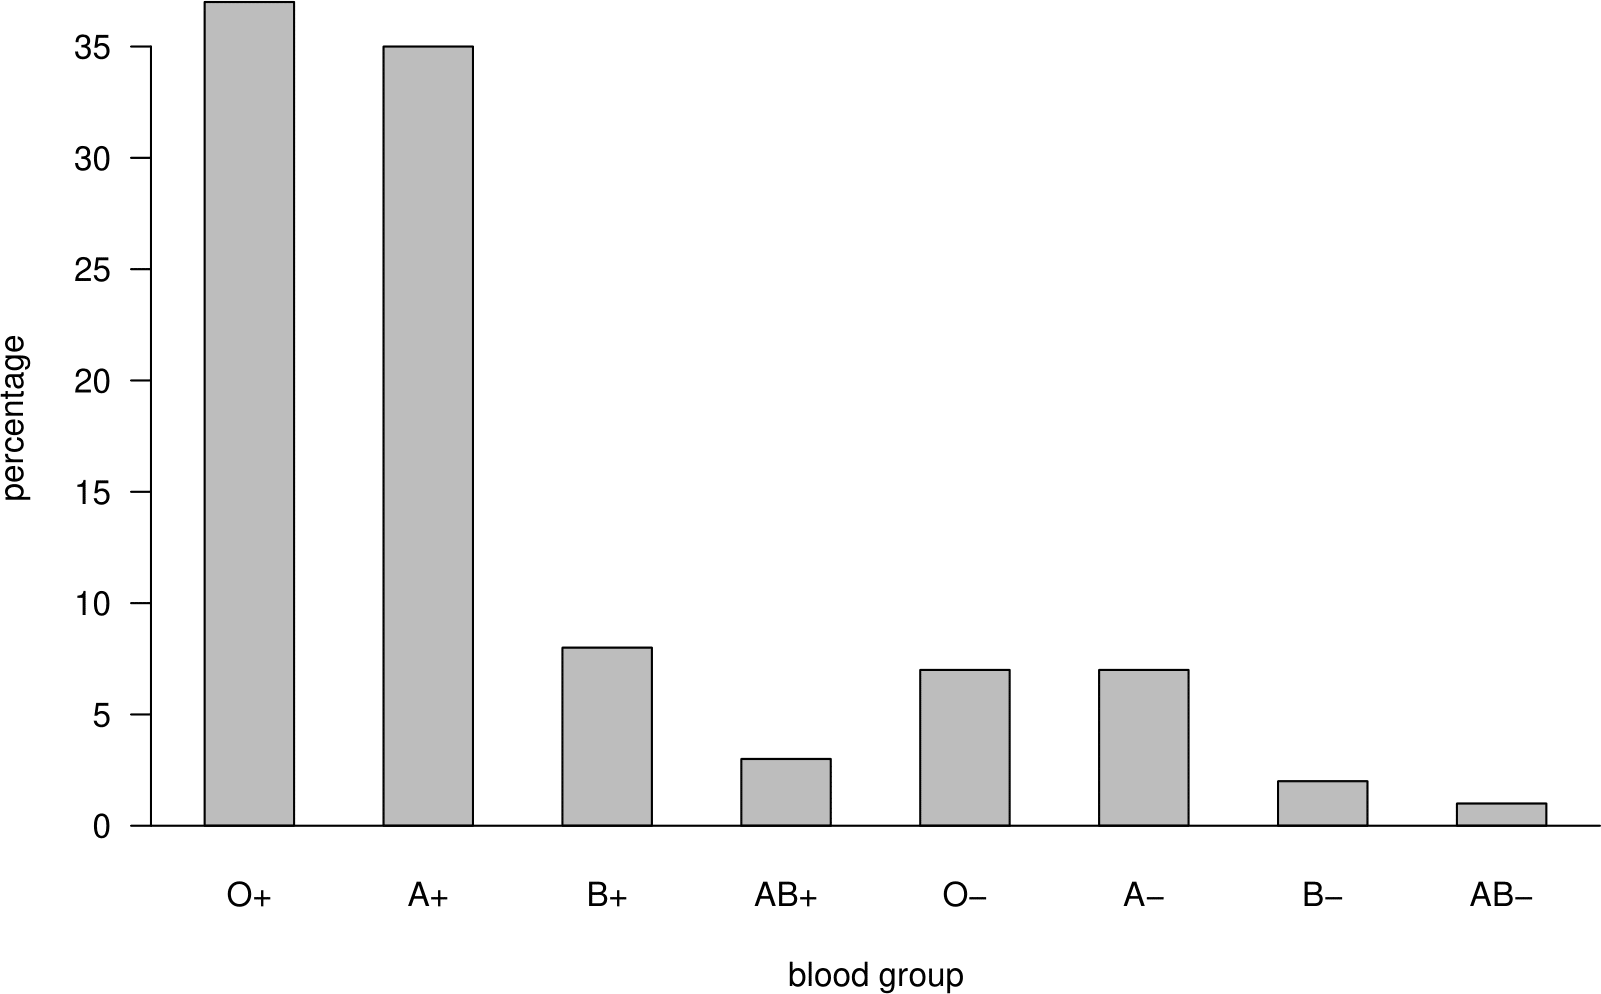
\includegraphics[width=0.6\linewidth]{images/ABO_barplots} 

}

\caption{Barplot of the UK ABO blood group percentages.}\label{fig:ABObar}
\end{figure}

\begin{figure}

{\centering 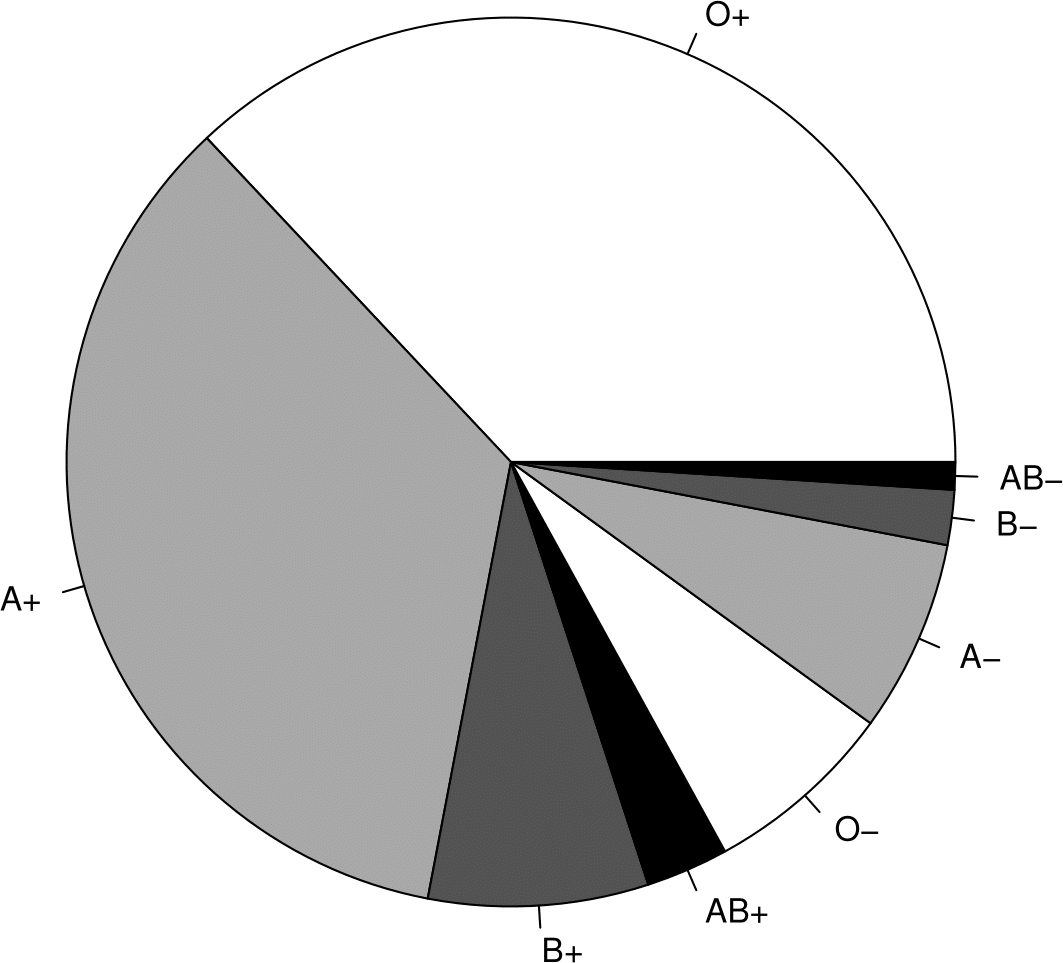
\includegraphics[width=0.75\linewidth]{images/ABO_pie} 

}

\caption{Pie chart (right) of the UK ABO blood group percentages.}\label{fig:ABOpie}
\end{figure}

\hypertarget{times-series-plots}{%
\subsection{Times series plots}\label{times-series-plots}}

The top plot of Figure \ref{fig:ftsenew} shows a \textbf{time series plot} (or time plot) of the weekly closing prices of the FTSE 100 share index from 2nd April 1984 to 13th August 2007. The bottom plot in this figure shows a different version of the same plot.

\begin{figure}

{\centering 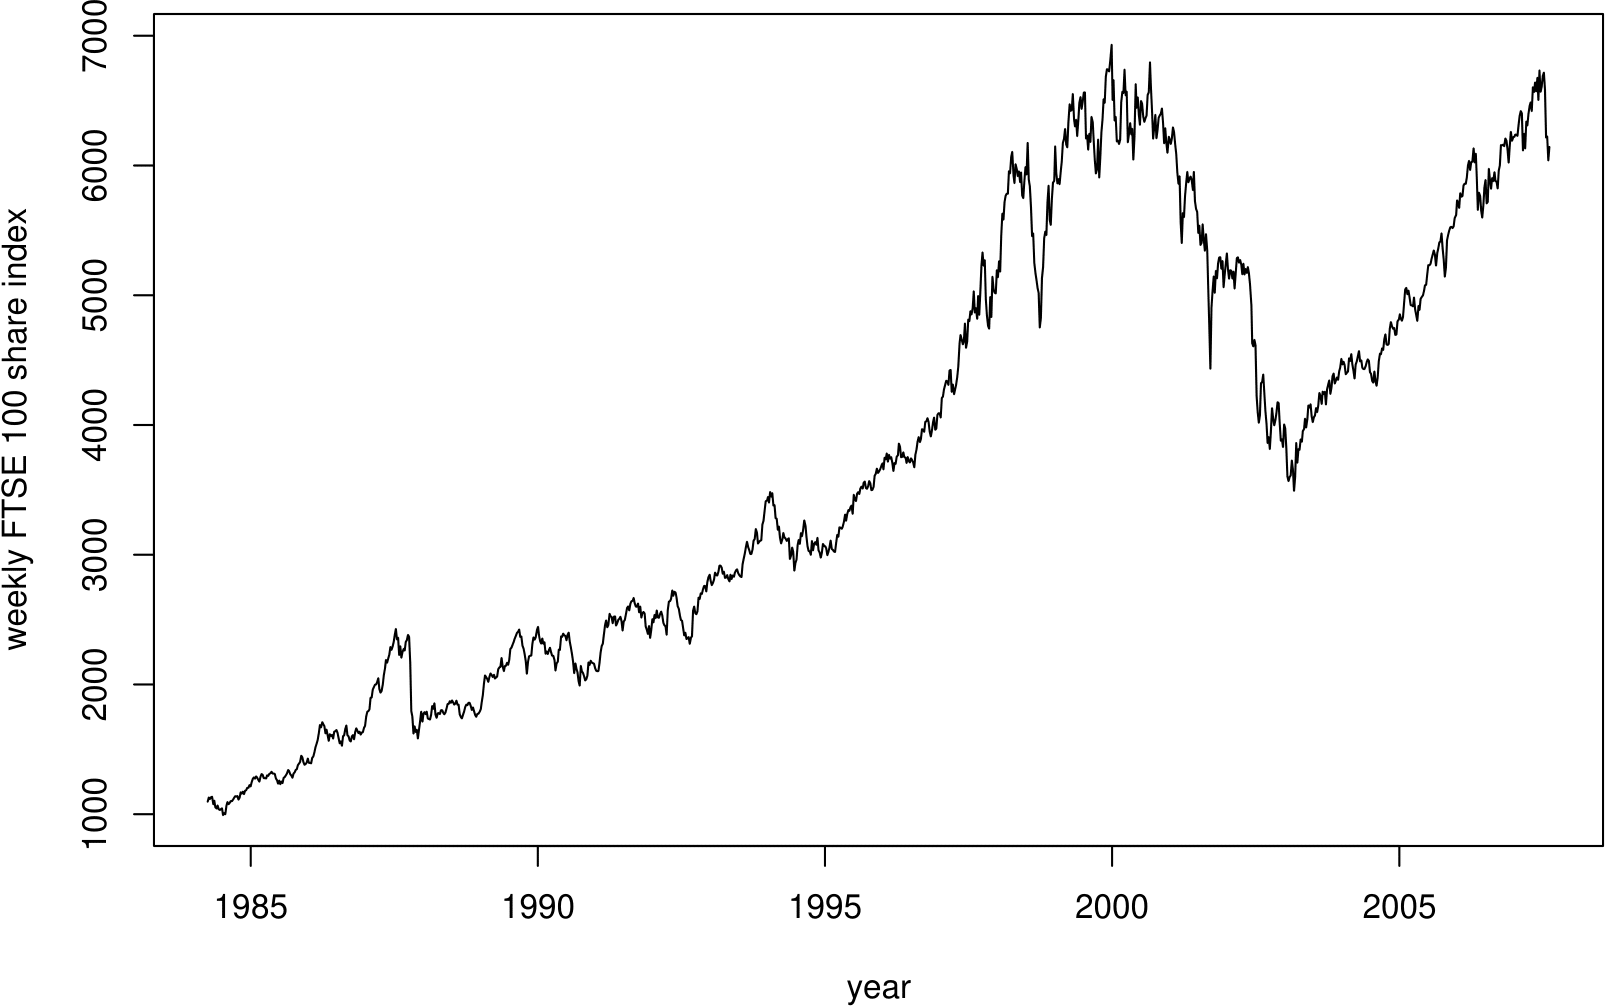
\includegraphics[width=0.75\linewidth]{images/ftse_weekly} 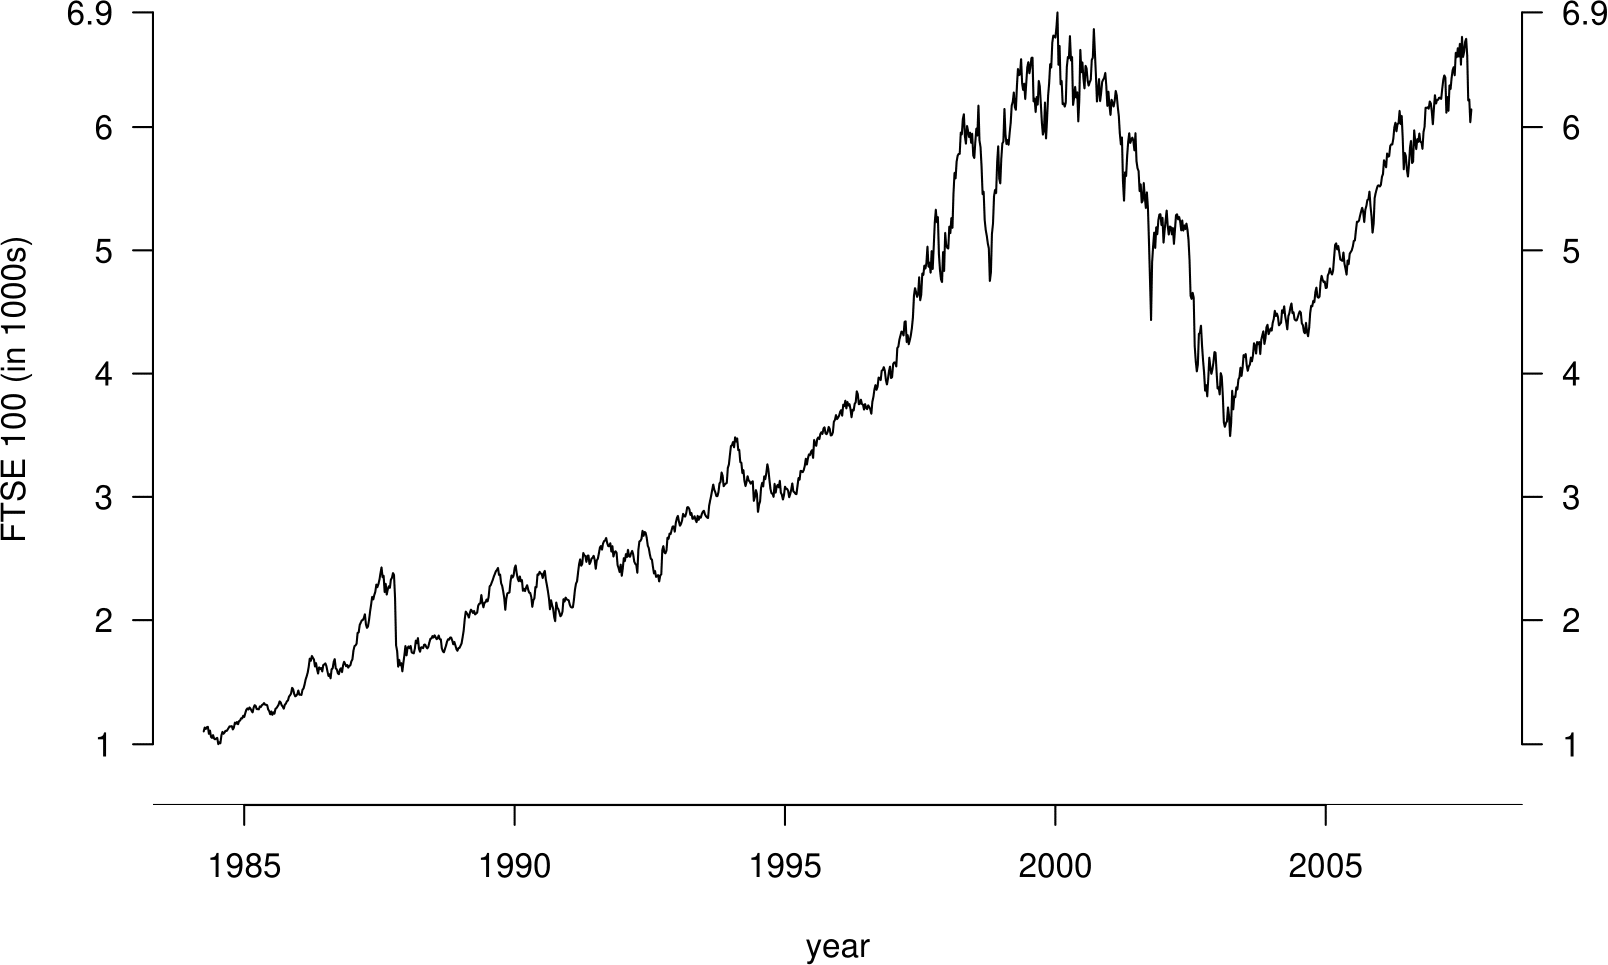
\includegraphics[width=0.75\linewidth]{images/ftse_weekly_tufte} 

}

\caption{Time series plots of the FTSE 100 weekly closing values, 1984--2007.  Top: default plot.  Bottom: modified version, with two vertical axes and the index measured in 1000s.}\label{fig:ftsenew}
\end{figure}

When observations are a time series, that is they are in time order, it is important to plot them against time to look for patterns. The sort of features that often turn up are upward or downward trends, or cyclical behaviour (alternative increases and decreases, often the result of seasonal behaviour),
but you may see other aspects worth noting. Note that

\begin{itemize}
\tightlist
\item
  time should be plotted on the horizontal axis;
\item
  the plot should be wider than it is high;
\item
  joining the dots can help to make interesting patterns easier to see.
\end{itemize}

Figure \ref{fig:fluts} shows a time series plot of another set of data. Can you guess what these data might be?

\begin{figure}

{\centering 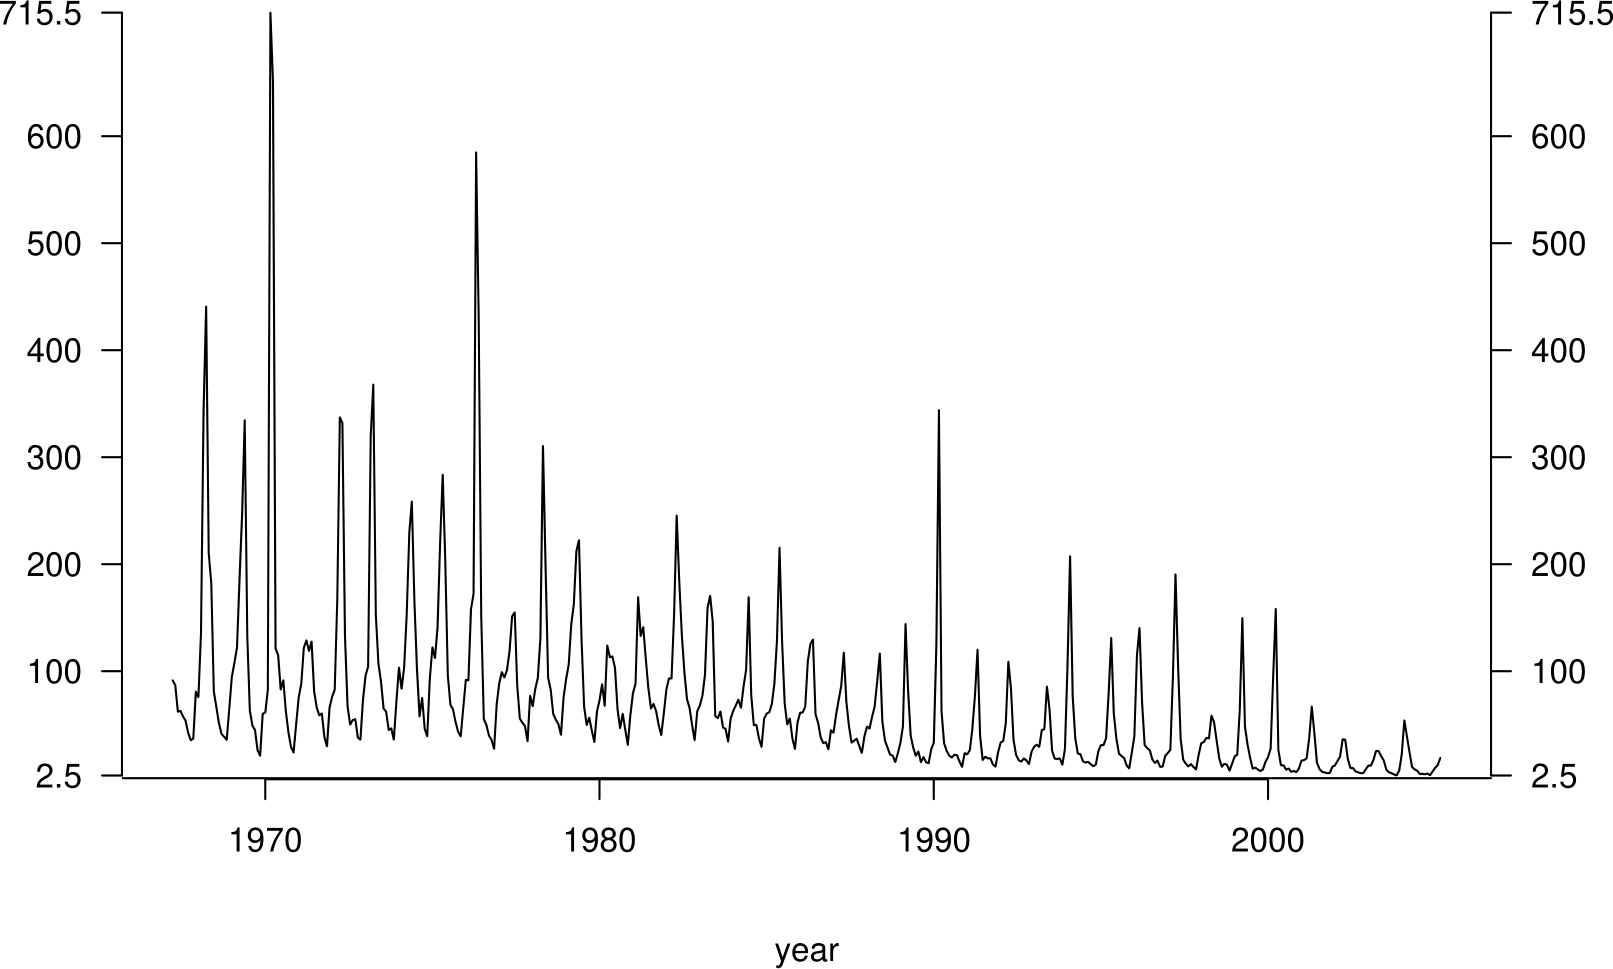
\includegraphics[width=0.75\linewidth]{images/flu_tufte_no_label} 

}

\caption{A time series plot of ?.}\label{fig:fluts}
\end{figure}

\hypertarget{election}{%
\section{2000 US Presidential Election}\label{election}}

Smith, R. L. (2002) \href{https://doi.org/10.1214/ss/1049993203}{A Statistical Assessment of Buchanan's Vote in Palm Beach County}. \emph{Statistcal Science}, \textbf{17}(4), 441--457.

In the 2000 U.S. Presidential election George W. Bush, the Republican candidate, narrowly beat Al Gore, the Democrat candidate. The result in the state of Florida was particularly close: Al Gore lost by only 537 votes out of 6 million votes cast. If Al Gore had won in Florida he would have become the U.S. President. After the election many allegations of voting irregularities were made and it was a month before Al Gore conceded defeat.

One of the results which caused most surprise was in Palm Beach County, Florida. Pat Buchanan, the Reform Party candidate, got an unexpectedly large 3,407 votes. Based on results in Florida as a whole only 1,300 votes would be expected. Also, given that Palm Beach is largely a Democratic County, a right-wing candidate such as Buchanan would expect even fewer votes.

In the days following the election it was suggested that the type of ballot paper, a so-called Butterfly Ballot \ref{fig:butterfly} used in Palm Beach had confused voters and lead to votes being cast for Buchanan by mistake. People found the Buchanan vote in Palm Beach surprising and there is a plausible explanation for how it occurred.

\begin{figure}

{\centering 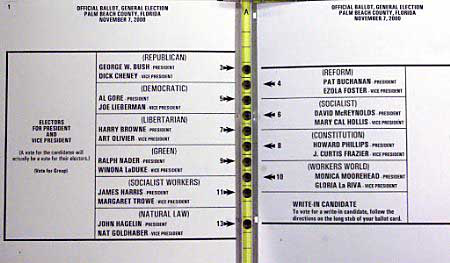
\includegraphics[width=0.75\linewidth]{images/butterflyballot} 

}

\caption{The Butterfly Ballot used in Palm Beach county.}\label{fig:butterfly}
\end{figure}

\citet{election} uses election results, and other data (on race, age, education and income), from Florida to answer the following questions:

\begin{enumerate}
\def\labelenumi{\arabic{enumi}.}
\tightlist
\item
  Is Buchanan's vote of 3,407 very clearly out of line with the pattern of results form the rest of Florida? In Statistics we call such data values \textbf{outliers}.
\item
  What level of vote for Buchanan would have been realistic in Palm Beach County?
\end{enumerate}

Figure \ref{fig:election1} suggests that the answer to question 1. is ``Yes''.

\begin{figure}

{\centering 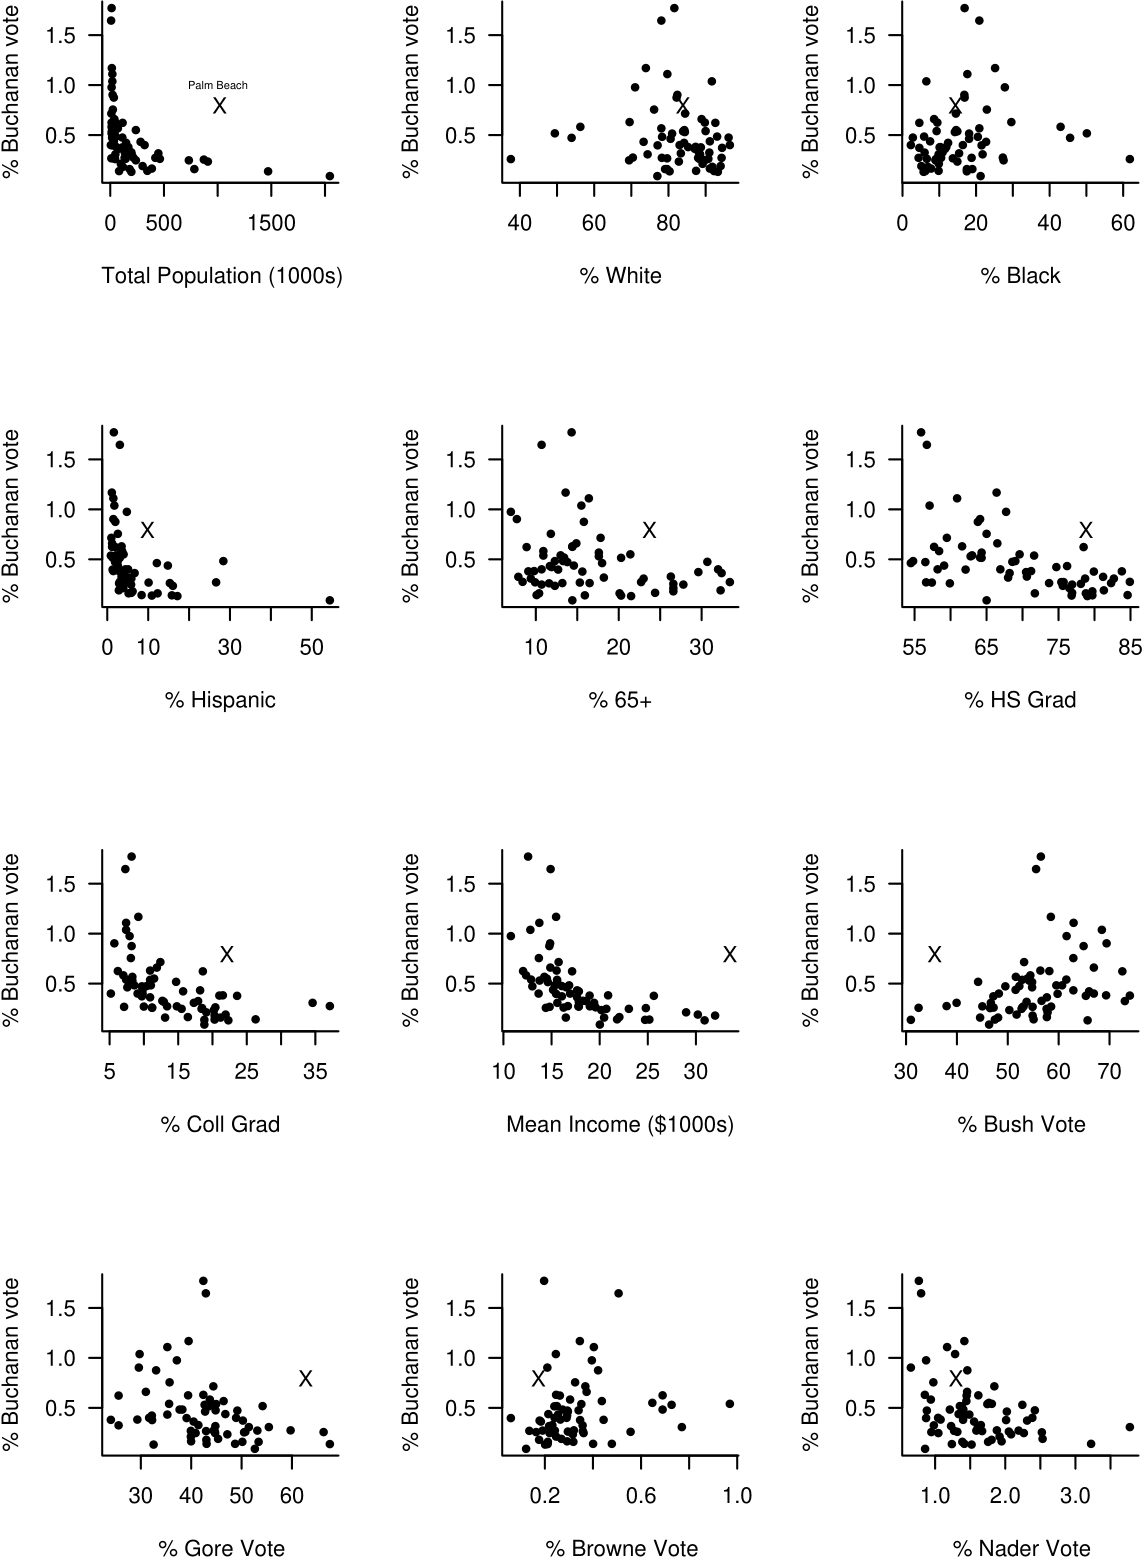
\includegraphics[width=0.75\linewidth]{images/election1} 

}

\caption{ Percentage of Buchanan votes against explanatory variables.  Palm Beach County is marked with a cross.}\label{fig:election1}
\end{figure}

On several of these plots Palm Beach stands out as a clear outlier. In these cases Buchanan gets many more votes than the pattern of the other points would suggest. We also see that the percentage of the vote that Buchanan gets tends to

\begin{itemize}
\tightlist
\item
  decrease with population size;
\item
  decrease with the percentage of of Hispanics;
\item
  decrease with the percentage of voters aged 65 or over;
\item
  decrease with high school and college graduation rate;
\item
  decrease with mean personal income;
\item
  decrease with the percentage of Gore votes;
\item
  increase with the percentage of Bush votes.
\end{itemize}

\citet{election} answers questions 1. and 2. more formally by building a linear regression model. This model quantifies how the percentage of Buchanan vote \(Y\), the \textbf{response variable}, depends on the other variables,the \textbf{explanatory variables} \(x_1,\ldots,x_{12}\). The general idea is to

\begin{itemize}
\tightlist
\item
  build the model using all the data for Florida, apart from the data from Palm Beach, using only the explanatory variables that have a significant effect;
\item
  predict the value of the Buchanan's vote in Palm Beach using the model.
\end{itemize}

We will study simple linear regression models (with only one explanatory variable) towards the end of STAT0002 (Chapter \ref{linreg}) and in STAT0003. The basic idea is to assume that a response variable has a linear (straight line) relationship with explanatory variables. The relationship will not be exact, so the model includes a \textbf{random error} term.

\citet{election} finds that transformations are required in order that the assumptions of the model are satisfied approximately. In particular he finds that using the response variable \(\sqrt{Y}\) is better than using \(Y\) itself (and better than other possible transformations). He also uses a \(\log_{10}\) transformation on some of the explanatory variables (for example Total Population), that is, he uses \(\log_{10}(x)\) rather than \(x\). Figure \ref{fig:election2} is a new version of figure \ref{fig:election1} in which the square root of the percentage of the vote obtained by Buchanan is plotted against the (possibly log-transformed) explanatory variables.

\citet{election} uses transformations of the original data in order to satisfy more closely the assumptions of the linear regression model:

\begin{itemize}
\tightlist
\item
  response = \(\sqrt{Y}\), instead of \(Y\);
\item
  for some explanatory variables, use \(\log_{10}(x)\) instead of \(x\).
\end{itemize}

\begin{figure}

{\centering 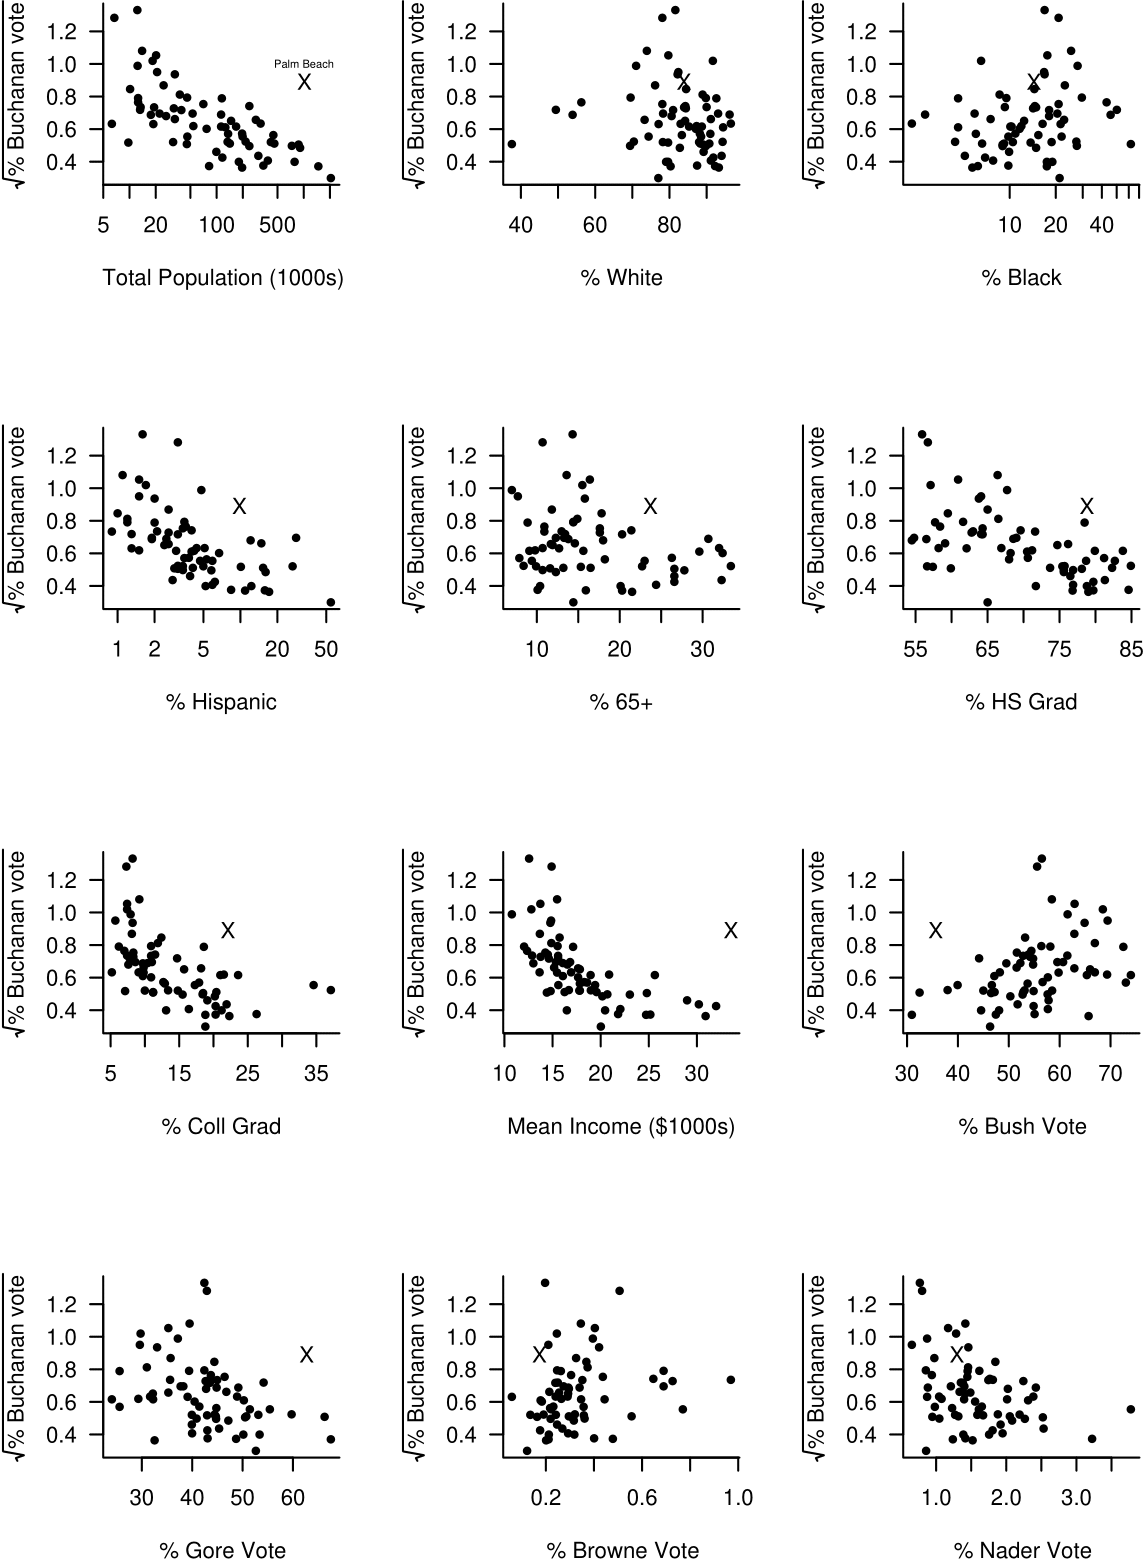
\includegraphics[width=0.75\linewidth]{images/election2} 

}

\caption{The square root of the percentage of Buchanan votes against explanatory variables.  Palm Beach County is marked with a cross.  Note the log scale on the $x$-axis of some plots.}\label{fig:election2}
\end{figure}

\hypertarget{log-scales-on-axes}{%
\subsubsection*{Log scales on axes}\label{log-scales-on-axes}}
\addcontentsline{toc}{subsubsection}{Log scales on axes}

Suppose that we produce a scatter plot where the data on the \(x\)-axis are 0.1, 1, 10, 100 and 1000. If we wish to plot \(\log_{10}(x)\) on the axis instead of \(x\) we have two choices:

\begin{enumerate}
\def\labelenumi{(\alph{enumi})}
\tightlist
\item
  Calculate \(\log_{10}(x)\) and plot these values on the axis.
\item
  Plot the values of \(x\) but on a \(\log_{10}\) scale. On a \(\log_{10}\) scale the values 0.1, 1, 10, 100 and 1000 are equally spaced. For example, from the basic rules of logs we have
  \[\log_{10}(10r) = \log_{10}(10)+\log_{10}(r)=1+\log_{10}(r).\]
  Therefore, on a \(\log_{10}\) scale the values \(10r\) and \(r\) are 1 unit apart. In other words adding 1 unit on a \(\log_{10}(x)\) scale corresponds to \textbf{multiplying} by 10 on the original \(x\)-scale.
\end{enumerate}

Both a. and b. will give exactly the same pattern of plot. The advantage of b. is that the original values are on the plot rather than the \(\log_{10}(x)\)
values. Figure \ref{fig:logaxes} illustrates this.

\begin{figure}

{\centering 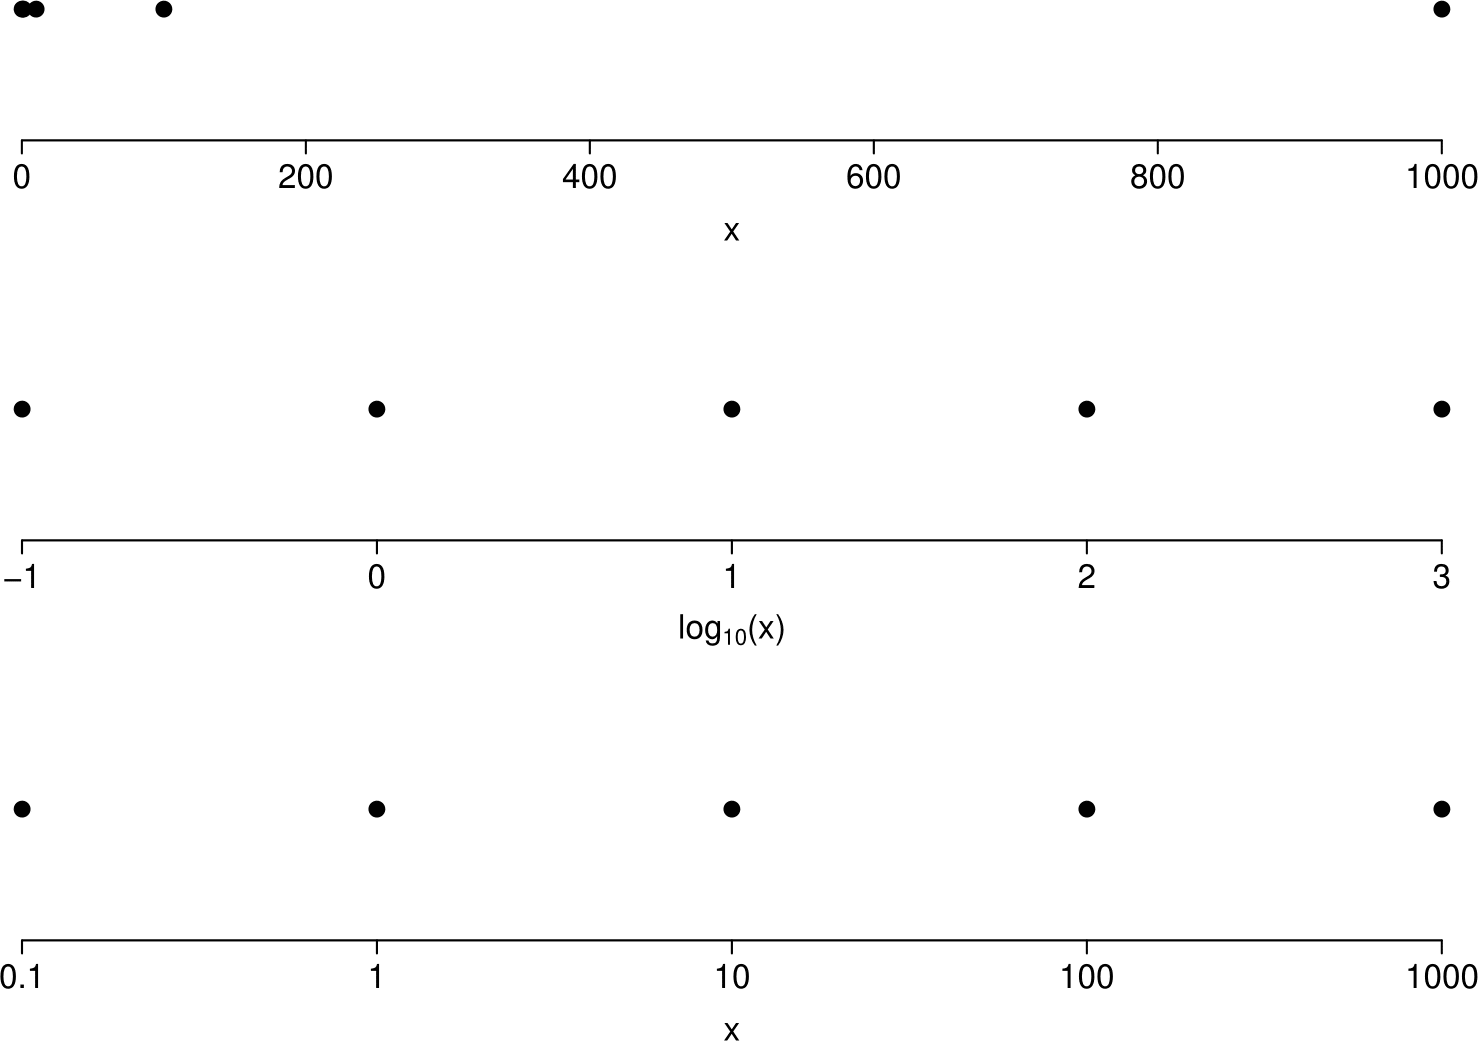
\includegraphics[width=0.75\linewidth]{images/log_axes} 

}

\caption{Plots to illustrate log-transformation of axes. Top: values of $x$ plotted. Middle: values of $\log_{10}(x)$ plotted. Bottom: values of $x$ plotted on a log-scale.}\label{fig:logaxes}
\end{figure}

Other notes on logs:

\begin{itemize}
\tightlist
\item
  we have used logs to base 10 for simplicity but the base doesn't matter;
\item
  logs are often helpful when the raw data are ratios (e.g.~\(x/y\)) or products (e.g.~\(xy\)). For example, exchange rates and price indices are ratios. If \(x=y\) then \(\log (x/y)=0\); if \(x=k\,y\) then \(\log (x/y)=\log k\); if \(y=k\,x\) then \(\log (x/y)=\log(1/k)=-\log k\); which is a nice symmetry.
\end{itemize}

Imagine that the model has only one explanatory variable, Total Population. You can imagine fitting this linear regression model as drawing a line of best fit through the points on the graph in the top left hand corner of figure \ref{fig:election2}. With more than one explanatory variable it is more complicated than this but the basic idea is the same.

After removing the Buchanan vote in Palm Beach (which we have decided is an outlier) \citet{election} finds that the model fits the data well.

The model predicts the Buchanan vote in Palm Beach to be 371, much lower than the official result of 3,407. This number (371) represents the `best guess' at the Buchanan vote given the other data. To show just how unlikely was the vote of 3,407, \citet{election} calculates a 95\% prediction interval of (219,534) for the Buchanan vote at Palm Beach. If the model is true, this interval has a probability of 95\% of containing the true value of the Buchanan vote.

Smith's analysis suggests that the true Buchanan vote should be approximately 3,000 votes lower than the official result. Given the design of the Butterfly Ballot it seems likely that most of these votes were intended for Al Gore. This would have given Gore the presidency instead of Bush.

\hypertarget{graphs2}{%
\section{Graphs (2 variables)}\label{graphs2}}

When we have 2 continuous variables it is common to examine the relationship between them using a \textbf{scatter plot}.

\hypertarget{scatter-plots}{%
\subsection{Scatter plots}\label{scatter-plots}}

We have already seen some scatter plots in the 2000 US Presidential Election example. We reproduce two of these plots in Figures \ref{fig:scatter1a} and \ref{fig:scatter1b}. A scatter plot is used to examine the relationship between two variables. We need the data to occur in pairs. In Figures \ref{fig:scatter1a} and \ref{fig:scatter1b} each county has a pair of observations: the percentage of votes for Buchanan and the value of the explanatory variable.

\begin{figure}

{\centering 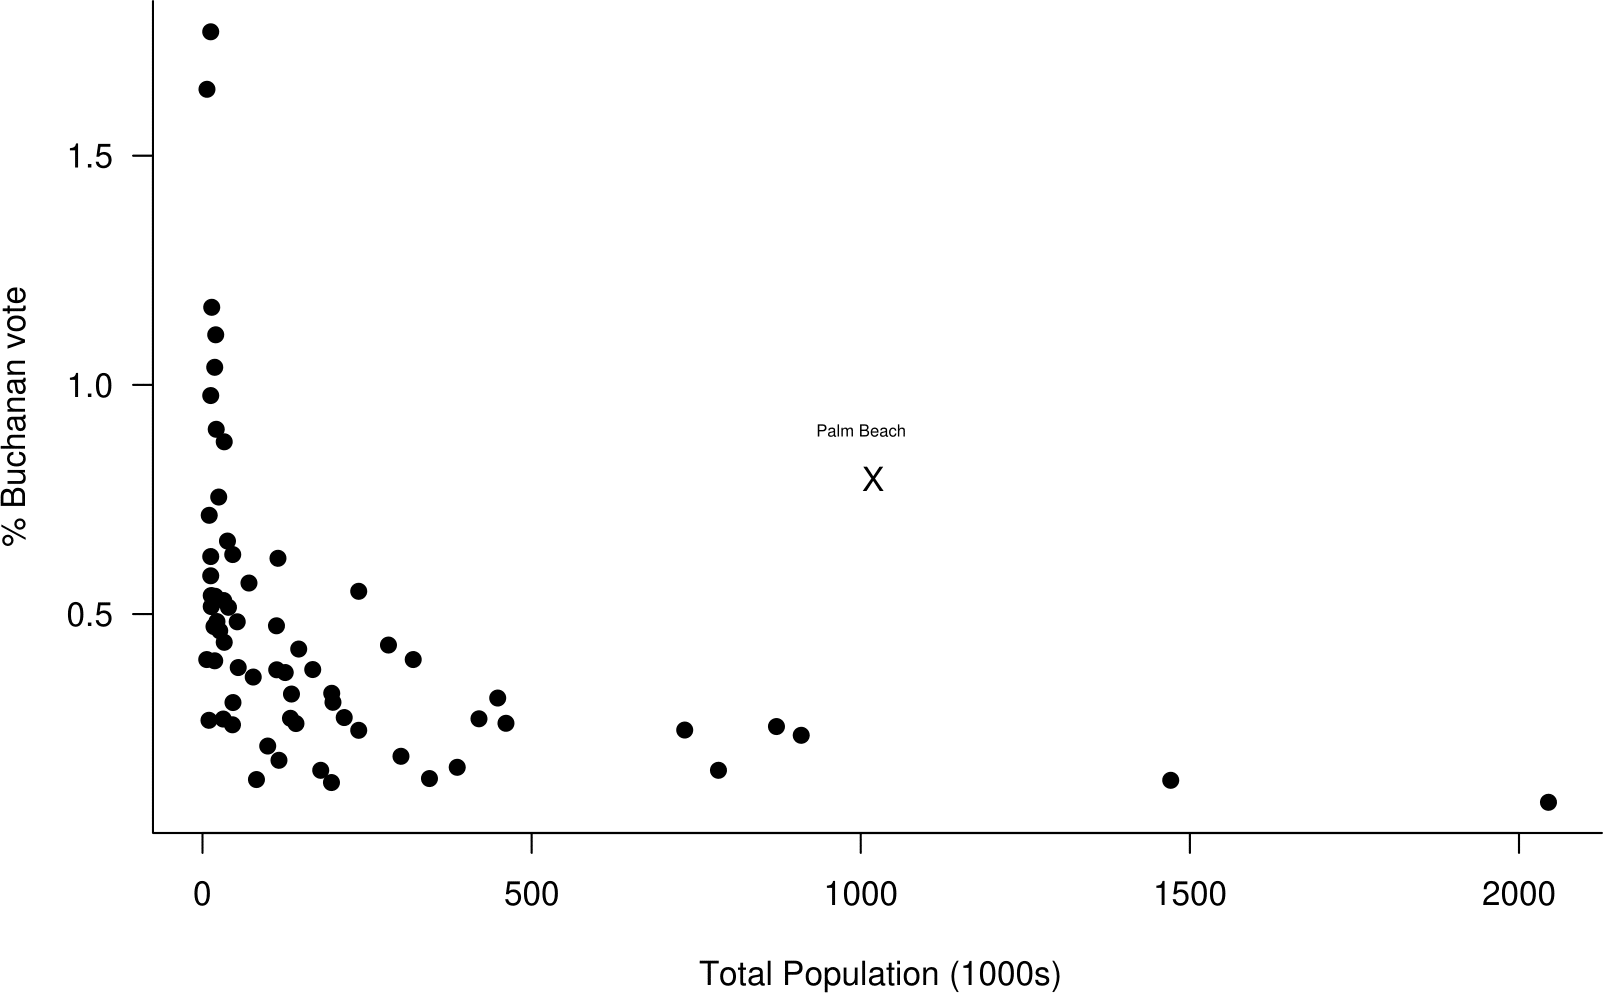
\includegraphics[width=0.75\linewidth]{images/election_scatter1a} 

}

\caption{Scatter plot of the percentage of the vote obtained by Buchanan against the total population from the 2000 US Presidential Election data.}\label{fig:scatter1a}
\end{figure}

\begin{figure}

{\centering 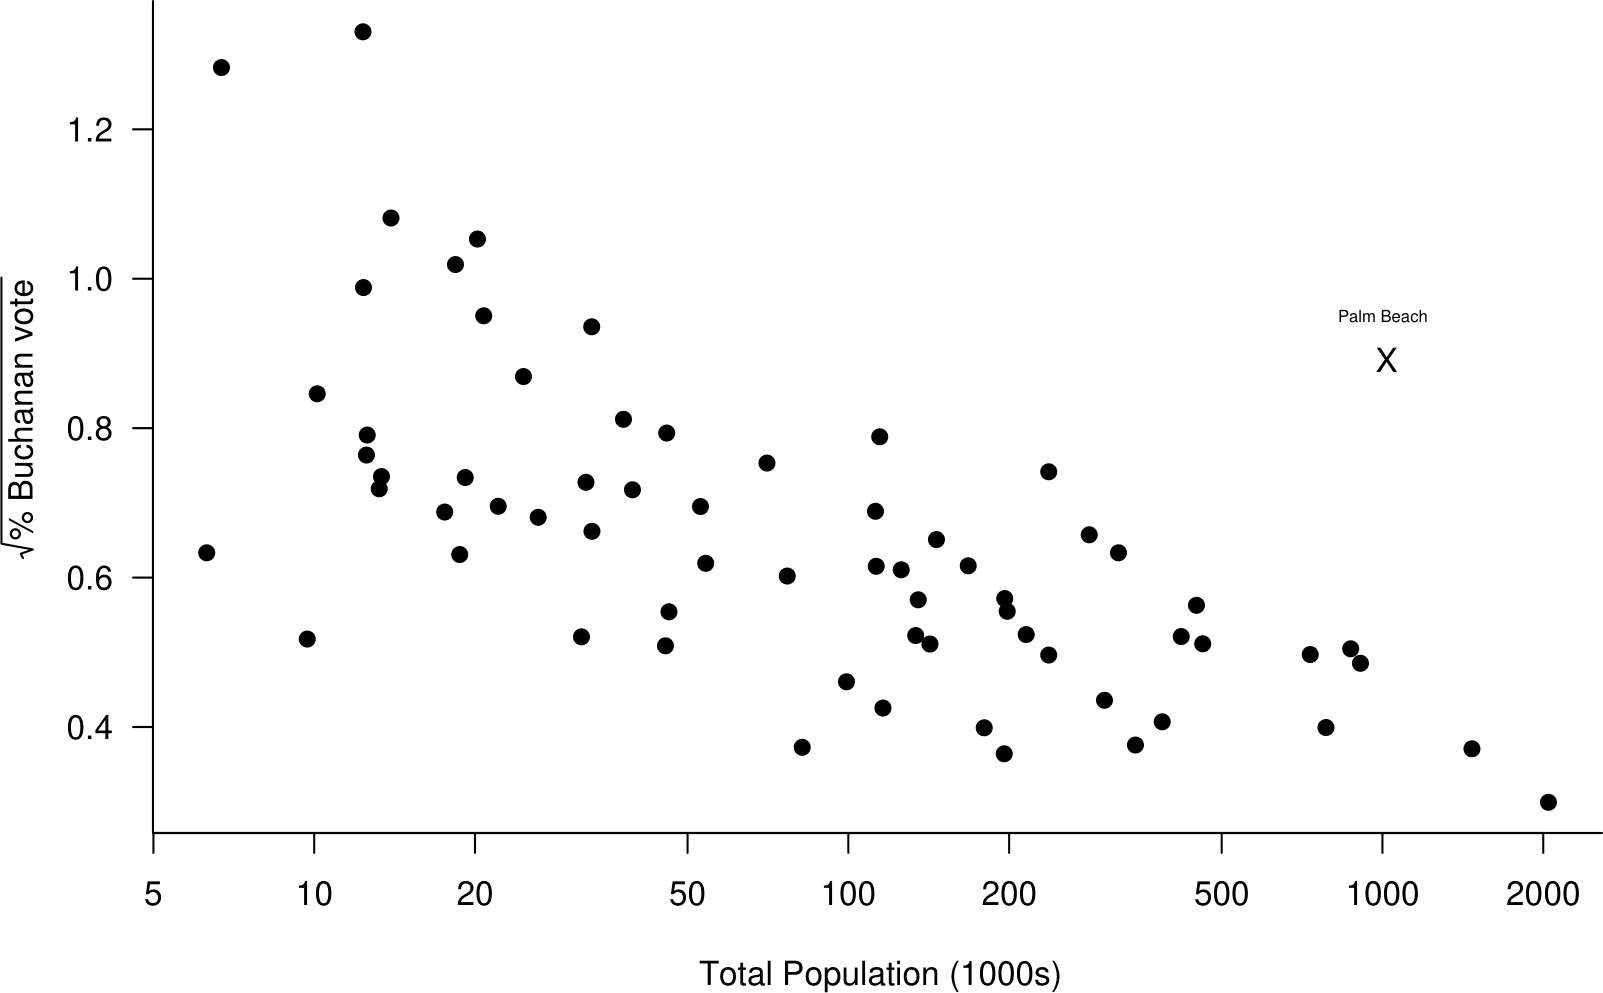
\includegraphics[width=0.75\linewidth]{images/election_scatter1b} 

}

\caption{Scatter plot of the square root of the percentage of the vote obtained by Buchanan against the log of the total population from the 2000 US Presidential Election data.  The plot suggests that these variables are aproximately linearly related.}\label{fig:scatter1b}
\end{figure}

Notice that we have plotted \% Buchanan vote (on the vertical \(y\)-axis) against total population (on the horizontal \(x\)-axis). This is because it makes sense that \% Buchanan vote depends on total population, that is, the size of population influences the vote, not the other way round.

Rules for deciding which variable to plot on the \(y\)-axis and which on the \(x\)-axis are:

\begin{itemize}
\tightlist
\item
  If the direction of dependence is clear, so that variable \(Y\) depends on variable \(X\). For example, \(X\)=river depth influencing \(Y\)=flow rate.
\item
  If one variable, \(X\), is fixed by an experimenter and then the value of another variable, \(Y\) is observed. For example, \(X\)=dosage of drug and \(Y\)=reduction in blood pressure.
\item
  If we wish to predict one variable, \(Y\), using another, \(X\). For example,
  \(X\)=share value today and \(Y\)=share value tomorrow.
\end{itemize}

It is clear in both these plots that the vote in Palm Beach is an outlier.
However, if we had produced separate plots of \% Buchanan vote and total
population Palm Beach would not appear as an outlier.

\hypertarget{transformation-of-data}{%
\section{Transformation of data}\label{transformation-of-data}}

Some simple statistical methods are based on assumptions about the statistical properties of the data to which they are applied. For example, there are methods that work well provided that a variable of interest is approximately symmetrically distributed. If a variable has a distribution that is strongly skewed then the method will not have the properties that are expected and the results may be misleading. In linear regression (see Chapter \ref{linreg}) the mean of one variable is represented as being related linearly to the value of another variable. If the reality is that this relationship is far from being linear then results may be very misleading.

If we wish to make use of simple assumptions like symmetry of distribution and/or linearity of relationship, but it is clear that the raw data do not support these assumption, then a legitimate approach is to consider whether the assumptions are satisfied better after we transform the data. We illustrate this idea in Sections \ref{transsymmetry} and \ref{straighten}.

\hypertarget{transsymmetry}{%
\subsection{Transformation to approximate symmetry}\label{transsymmetry}}

The data in Table \ref{tab:clouds} resulted from an experiment (\citet{clouds}) to see whether spraying silver nitrate into a cloud (known as \textbf{seeding} the cloud)
could make it produce more rainfall. 52 clouds were studied. 26 of the clouds were chosen at random and seeded with silver nitrate. The amounts of rainfall, in acre-feet, produced by each cloud is recorded. (An acre-foot is a unit of volume equal to 43,560 feet\(^3\) or, approximately, 1233.5m\(^3\).)

 
  \providecommand{\huxb}[2]{\arrayrulecolor[RGB]{#1}\global\arrayrulewidth=#2pt}
  \providecommand{\huxvb}[2]{\color[RGB]{#1}\vrule width #2pt}
  \providecommand{\huxtpad}[1]{\rule{0pt}{#1}}
  \providecommand{\huxbpad}[1]{\rule[-#1]{0pt}{#1}}

\begin{table}[ht]
\begin{centerbox}
\begin{threeparttable}
\captionsetup{justification=centering,singlelinecheck=off}
\caption{\label{tab:clouds} The rainfall, in acre-feet, from 52 clouds, 26 of which were chosen at random to be seeded with silver nitrate.}
 \setlength{\tabcolsep}{0pt}
\begin{tabularx}{0.75\textwidth}{p{0.1875\textwidth} p{0.1875\textwidth} p{0.1875\textwidth} p{0.1875\textwidth}}


\hhline{>{\huxb{0, 0, 0}{1}}->{\huxb{0, 0, 0}{1}}->{\huxb{0, 0, 0}{1}}->{\huxb{0, 0, 0}{1}}-}
\arrayrulecolor{black}

\multicolumn{2}{!{\huxvb{0, 0, 0}{1}}p{0.375\textwidth+2\tabcolsep}!{\huxvb{0, 0, 0}{4}}!{\huxvb{0, 0, 0}{4}}}{\cellcolor[RGB]{255, 255, 255}\hspace{0pt}\parbox[b]{0.375\textwidth+2\tabcolsep-0pt-6pt}{\huxtpad{0pt + 1em}\centering unseeded\huxbpad{0pt}}} &
\multicolumn{2}{p{0.375\textwidth+2\tabcolsep}!{\huxvb{0, 0, 0}{1}}}{\cellcolor[RGB]{255, 255, 255}\hspace{0pt}\parbox[b]{0.375\textwidth+2\tabcolsep-0pt-6pt}{\huxtpad{0pt + 1em}\centering seeded\huxbpad{0pt}}} \tabularnewline[-0.5pt]


\hhline{>{\huxb{0, 0, 0}{1}}->{\huxb{0, 0, 0}{1}}->{\huxb{0, 0, 0}{1}}->{\huxb{0, 0, 0}{1}}-}
\arrayrulecolor{black}

\multicolumn{1}{!{\huxvb{0, 0, 0}{1}}p{0.1875\textwidth}!{\huxvb{0, 0, 0}{1}}}{\cellcolor[RGB]{255, 255, 255}\hspace{0pt}\parbox[b]{0.1875\textwidth-0pt-35pt}{\huxtpad{0pt + 1em}\raggedleft 1202.6\huxbpad{0pt}}} &
\multicolumn{1}{p{0.1875\textwidth}!{\huxvb{0, 0, 0}{4}}!{\huxvb{0, 0, 0}{4}}}{\cellcolor[RGB]{255, 255, 255}\hspace{0pt}\parbox[b]{0.1875\textwidth-0pt-35pt}{\huxtpad{0pt + 1em}\raggedleft 41.1\huxbpad{0pt}}} &
\multicolumn{1}{p{0.1875\textwidth}!{\huxvb{0, 0, 0}{1}}}{\cellcolor[RGB]{255, 255, 255}\hspace{0pt}\parbox[b]{0.1875\textwidth-0pt-35pt}{\huxtpad{0pt + 1em}\raggedleft 2745.6\huxbpad{0pt}}} &
\multicolumn{1}{p{0.1875\textwidth}!{\huxvb{0, 0, 0}{1}}}{\cellcolor[RGB]{255, 255, 255}\hspace{0pt}\parbox[b]{0.1875\textwidth-0pt-35pt}{\huxtpad{0pt + 1em}\raggedleft 200.7\huxbpad{0pt}}} \tabularnewline[-0.5pt]


\hhline{>{\huxb{255, 255, 255}{0.1}}->{\huxb{255, 255, 255}{0.1}}->{\huxb{255, 255, 255}{0.1}}->{\huxb{255, 255, 255}{0.1}}-}
\arrayrulecolor{black}

\multicolumn{1}{!{\huxvb{0, 0, 0}{1}}p{0.1875\textwidth}!{\huxvb{0, 0, 0}{1}}}{\cellcolor[RGB]{255, 255, 255}\hspace{0pt}\parbox[b]{0.1875\textwidth-0pt-35pt}{\huxtpad{0pt + 1em}\raggedleft 830.1\huxbpad{0pt}}} &
\multicolumn{1}{p{0.1875\textwidth}!{\huxvb{0, 0, 0}{4}}!{\huxvb{0, 0, 0}{4}}}{\cellcolor[RGB]{255, 255, 255}\hspace{0pt}\parbox[b]{0.1875\textwidth-0pt-35pt}{\huxtpad{0pt + 1em}\raggedleft 36.6\huxbpad{0pt}}} &
\multicolumn{1}{p{0.1875\textwidth}!{\huxvb{0, 0, 0}{1}}}{\cellcolor[RGB]{255, 255, 255}\hspace{0pt}\parbox[b]{0.1875\textwidth-0pt-35pt}{\huxtpad{0pt + 1em}\raggedleft 1697.8\huxbpad{0pt}}} &
\multicolumn{1}{p{0.1875\textwidth}!{\huxvb{0, 0, 0}{1}}}{\cellcolor[RGB]{255, 255, 255}\hspace{0pt}\parbox[b]{0.1875\textwidth-0pt-35pt}{\huxtpad{0pt + 1em}\raggedleft 198.6\huxbpad{0pt}}} \tabularnewline[-0.5pt]


\hhline{>{\huxb{255, 255, 255}{0.1}}->{\huxb{255, 255, 255}{0.1}}->{\huxb{255, 255, 255}{0.1}}->{\huxb{255, 255, 255}{0.1}}-}
\arrayrulecolor{black}

\multicolumn{1}{!{\huxvb{0, 0, 0}{1}}p{0.1875\textwidth}!{\huxvb{0, 0, 0}{1}}}{\cellcolor[RGB]{255, 255, 255}\hspace{0pt}\parbox[b]{0.1875\textwidth-0pt-35pt}{\huxtpad{0pt + 1em}\raggedleft 372.4\huxbpad{0pt}}} &
\multicolumn{1}{p{0.1875\textwidth}!{\huxvb{0, 0, 0}{4}}!{\huxvb{0, 0, 0}{4}}}{\cellcolor[RGB]{255, 255, 255}\hspace{0pt}\parbox[b]{0.1875\textwidth-0pt-35pt}{\huxtpad{0pt + 1em}\raggedleft 29.0\huxbpad{0pt}}} &
\multicolumn{1}{p{0.1875\textwidth}!{\huxvb{0, 0, 0}{1}}}{\cellcolor[RGB]{255, 255, 255}\hspace{0pt}\parbox[b]{0.1875\textwidth-0pt-35pt}{\huxtpad{0pt + 1em}\raggedleft 1656.0\huxbpad{0pt}}} &
\multicolumn{1}{p{0.1875\textwidth}!{\huxvb{0, 0, 0}{1}}}{\cellcolor[RGB]{255, 255, 255}\hspace{0pt}\parbox[b]{0.1875\textwidth-0pt-35pt}{\huxtpad{0pt + 1em}\raggedleft 129.6\huxbpad{0pt}}} \tabularnewline[-0.5pt]


\hhline{>{\huxb{255, 255, 255}{0.1}}->{\huxb{255, 255, 255}{0.1}}->{\huxb{255, 255, 255}{0.1}}->{\huxb{255, 255, 255}{0.1}}-}
\arrayrulecolor{black}

\multicolumn{1}{!{\huxvb{0, 0, 0}{1}}p{0.1875\textwidth}!{\huxvb{0, 0, 0}{1}}}{\cellcolor[RGB]{255, 255, 255}\hspace{0pt}\parbox[b]{0.1875\textwidth-0pt-35pt}{\huxtpad{0pt + 1em}\raggedleft 345.5\huxbpad{0pt}}} &
\multicolumn{1}{p{0.1875\textwidth}!{\huxvb{0, 0, 0}{4}}!{\huxvb{0, 0, 0}{4}}}{\cellcolor[RGB]{255, 255, 255}\hspace{0pt}\parbox[b]{0.1875\textwidth-0pt-35pt}{\huxtpad{0pt + 1em}\raggedleft 28.6\huxbpad{0pt}}} &
\multicolumn{1}{p{0.1875\textwidth}!{\huxvb{0, 0, 0}{1}}}{\cellcolor[RGB]{255, 255, 255}\hspace{0pt}\parbox[b]{0.1875\textwidth-0pt-35pt}{\huxtpad{0pt + 1em}\raggedleft 978.0\huxbpad{0pt}}} &
\multicolumn{1}{p{0.1875\textwidth}!{\huxvb{0, 0, 0}{1}}}{\cellcolor[RGB]{255, 255, 255}\hspace{0pt}\parbox[b]{0.1875\textwidth-0pt-35pt}{\huxtpad{0pt + 1em}\raggedleft 119.0\huxbpad{0pt}}} \tabularnewline[-0.5pt]


\hhline{>{\huxb{255, 255, 255}{0.1}}->{\huxb{255, 255, 255}{0.1}}->{\huxb{255, 255, 255}{0.1}}->{\huxb{255, 255, 255}{0.1}}-}
\arrayrulecolor{black}

\multicolumn{1}{!{\huxvb{0, 0, 0}{1}}p{0.1875\textwidth}!{\huxvb{0, 0, 0}{1}}}{\cellcolor[RGB]{255, 255, 255}\hspace{0pt}\parbox[b]{0.1875\textwidth-0pt-35pt}{\huxtpad{0pt + 1em}\raggedleft 321.2\huxbpad{0pt}}} &
\multicolumn{1}{p{0.1875\textwidth}!{\huxvb{0, 0, 0}{4}}!{\huxvb{0, 0, 0}{4}}}{\cellcolor[RGB]{255, 255, 255}\hspace{0pt}\parbox[b]{0.1875\textwidth-0pt-35pt}{\huxtpad{0pt + 1em}\raggedleft 26.3\huxbpad{0pt}}} &
\multicolumn{1}{p{0.1875\textwidth}!{\huxvb{0, 0, 0}{1}}}{\cellcolor[RGB]{255, 255, 255}\hspace{0pt}\parbox[b]{0.1875\textwidth-0pt-35pt}{\huxtpad{0pt + 1em}\raggedleft 703.4\huxbpad{0pt}}} &
\multicolumn{1}{p{0.1875\textwidth}!{\huxvb{0, 0, 0}{1}}}{\cellcolor[RGB]{255, 255, 255}\hspace{0pt}\parbox[b]{0.1875\textwidth-0pt-35pt}{\huxtpad{0pt + 1em}\raggedleft 118.3\huxbpad{0pt}}} \tabularnewline[-0.5pt]


\hhline{>{\huxb{255, 255, 255}{0.1}}->{\huxb{255, 255, 255}{0.1}}->{\huxb{255, 255, 255}{0.1}}->{\huxb{255, 255, 255}{0.1}}-}
\arrayrulecolor{black}

\multicolumn{1}{!{\huxvb{0, 0, 0}{1}}p{0.1875\textwidth}!{\huxvb{0, 0, 0}{1}}}{\cellcolor[RGB]{255, 255, 255}\hspace{0pt}\parbox[b]{0.1875\textwidth-0pt-35pt}{\huxtpad{0pt + 1em}\raggedleft 244.3\huxbpad{0pt}}} &
\multicolumn{1}{p{0.1875\textwidth}!{\huxvb{0, 0, 0}{4}}!{\huxvb{0, 0, 0}{4}}}{\cellcolor[RGB]{255, 255, 255}\hspace{0pt}\parbox[b]{0.1875\textwidth-0pt-35pt}{\huxtpad{0pt + 1em}\raggedleft 26.1\huxbpad{0pt}}} &
\multicolumn{1}{p{0.1875\textwidth}!{\huxvb{0, 0, 0}{1}}}{\cellcolor[RGB]{255, 255, 255}\hspace{0pt}\parbox[b]{0.1875\textwidth-0pt-35pt}{\huxtpad{0pt + 1em}\raggedleft 489.1\huxbpad{0pt}}} &
\multicolumn{1}{p{0.1875\textwidth}!{\huxvb{0, 0, 0}{1}}}{\cellcolor[RGB]{255, 255, 255}\hspace{0pt}\parbox[b]{0.1875\textwidth-0pt-35pt}{\huxtpad{0pt + 1em}\raggedleft 115.3\huxbpad{0pt}}} \tabularnewline[-0.5pt]


\hhline{>{\huxb{255, 255, 255}{0.1}}->{\huxb{255, 255, 255}{0.1}}->{\huxb{255, 255, 255}{0.1}}->{\huxb{255, 255, 255}{0.1}}-}
\arrayrulecolor{black}

\multicolumn{1}{!{\huxvb{0, 0, 0}{1}}p{0.1875\textwidth}!{\huxvb{0, 0, 0}{1}}}{\cellcolor[RGB]{255, 255, 255}\hspace{0pt}\parbox[b]{0.1875\textwidth-0pt-35pt}{\huxtpad{0pt + 1em}\raggedleft 163.0\huxbpad{0pt}}} &
\multicolumn{1}{p{0.1875\textwidth}!{\huxvb{0, 0, 0}{4}}!{\huxvb{0, 0, 0}{4}}}{\cellcolor[RGB]{255, 255, 255}\hspace{0pt}\parbox[b]{0.1875\textwidth-0pt-35pt}{\huxtpad{0pt + 1em}\raggedleft 24.4\huxbpad{0pt}}} &
\multicolumn{1}{p{0.1875\textwidth}!{\huxvb{0, 0, 0}{1}}}{\cellcolor[RGB]{255, 255, 255}\hspace{0pt}\parbox[b]{0.1875\textwidth-0pt-35pt}{\huxtpad{0pt + 1em}\raggedleft 430.0\huxbpad{0pt}}} &
\multicolumn{1}{p{0.1875\textwidth}!{\huxvb{0, 0, 0}{1}}}{\cellcolor[RGB]{255, 255, 255}\hspace{0pt}\parbox[b]{0.1875\textwidth-0pt-35pt}{\huxtpad{0pt + 1em}\raggedleft 92.4\huxbpad{0pt}}} \tabularnewline[-0.5pt]


\hhline{>{\huxb{255, 255, 255}{0.1}}->{\huxb{255, 255, 255}{0.1}}->{\huxb{255, 255, 255}{0.1}}->{\huxb{255, 255, 255}{0.1}}-}
\arrayrulecolor{black}

\multicolumn{1}{!{\huxvb{0, 0, 0}{1}}p{0.1875\textwidth}!{\huxvb{0, 0, 0}{1}}}{\cellcolor[RGB]{255, 255, 255}\hspace{0pt}\parbox[b]{0.1875\textwidth-0pt-35pt}{\huxtpad{0pt + 1em}\raggedleft 147.8\huxbpad{0pt}}} &
\multicolumn{1}{p{0.1875\textwidth}!{\huxvb{0, 0, 0}{4}}!{\huxvb{0, 0, 0}{4}}}{\cellcolor[RGB]{255, 255, 255}\hspace{0pt}\parbox[b]{0.1875\textwidth-0pt-35pt}{\huxtpad{0pt + 1em}\raggedleft 21.7\huxbpad{0pt}}} &
\multicolumn{1}{p{0.1875\textwidth}!{\huxvb{0, 0, 0}{1}}}{\cellcolor[RGB]{255, 255, 255}\hspace{0pt}\parbox[b]{0.1875\textwidth-0pt-35pt}{\huxtpad{0pt + 1em}\raggedleft 334.1\huxbpad{0pt}}} &
\multicolumn{1}{p{0.1875\textwidth}!{\huxvb{0, 0, 0}{1}}}{\cellcolor[RGB]{255, 255, 255}\hspace{0pt}\parbox[b]{0.1875\textwidth-0pt-35pt}{\huxtpad{0pt + 1em}\raggedleft 40.6\huxbpad{0pt}}} \tabularnewline[-0.5pt]


\hhline{>{\huxb{255, 255, 255}{0.1}}->{\huxb{255, 255, 255}{0.1}}->{\huxb{255, 255, 255}{0.1}}->{\huxb{255, 255, 255}{0.1}}-}
\arrayrulecolor{black}

\multicolumn{1}{!{\huxvb{0, 0, 0}{1}}p{0.1875\textwidth}!{\huxvb{0, 0, 0}{1}}}{\cellcolor[RGB]{255, 255, 255}\hspace{0pt}\parbox[b]{0.1875\textwidth-0pt-35pt}{\huxtpad{0pt + 1em}\raggedleft 95.0\huxbpad{0pt}}} &
\multicolumn{1}{p{0.1875\textwidth}!{\huxvb{0, 0, 0}{4}}!{\huxvb{0, 0, 0}{4}}}{\cellcolor[RGB]{255, 255, 255}\hspace{0pt}\parbox[b]{0.1875\textwidth-0pt-35pt}{\huxtpad{0pt + 1em}\raggedleft 17.3\huxbpad{0pt}}} &
\multicolumn{1}{p{0.1875\textwidth}!{\huxvb{0, 0, 0}{1}}}{\cellcolor[RGB]{255, 255, 255}\hspace{0pt}\parbox[b]{0.1875\textwidth-0pt-35pt}{\huxtpad{0pt + 1em}\raggedleft 302.8\huxbpad{0pt}}} &
\multicolumn{1}{p{0.1875\textwidth}!{\huxvb{0, 0, 0}{1}}}{\cellcolor[RGB]{255, 255, 255}\hspace{0pt}\parbox[b]{0.1875\textwidth-0pt-35pt}{\huxtpad{0pt + 1em}\raggedleft 32.7\huxbpad{0pt}}} \tabularnewline[-0.5pt]


\hhline{>{\huxb{255, 255, 255}{0.1}}->{\huxb{255, 255, 255}{0.1}}->{\huxb{255, 255, 255}{0.1}}->{\huxb{255, 255, 255}{0.1}}-}
\arrayrulecolor{black}

\multicolumn{1}{!{\huxvb{0, 0, 0}{1}}p{0.1875\textwidth}!{\huxvb{0, 0, 0}{1}}}{\cellcolor[RGB]{255, 255, 255}\hspace{0pt}\parbox[b]{0.1875\textwidth-0pt-35pt}{\huxtpad{0pt + 1em}\raggedleft 87.0\huxbpad{0pt}}} &
\multicolumn{1}{p{0.1875\textwidth}!{\huxvb{0, 0, 0}{4}}!{\huxvb{0, 0, 0}{4}}}{\cellcolor[RGB]{255, 255, 255}\hspace{0pt}\parbox[b]{0.1875\textwidth-0pt-35pt}{\huxtpad{0pt + 1em}\raggedleft 11.5\huxbpad{0pt}}} &
\multicolumn{1}{p{0.1875\textwidth}!{\huxvb{0, 0, 0}{1}}}{\cellcolor[RGB]{255, 255, 255}\hspace{0pt}\parbox[b]{0.1875\textwidth-0pt-35pt}{\huxtpad{0pt + 1em}\raggedleft 274.7\huxbpad{0pt}}} &
\multicolumn{1}{p{0.1875\textwidth}!{\huxvb{0, 0, 0}{1}}}{\cellcolor[RGB]{255, 255, 255}\hspace{0pt}\parbox[b]{0.1875\textwidth-0pt-35pt}{\huxtpad{0pt + 1em}\raggedleft 31.4\huxbpad{0pt}}} \tabularnewline[-0.5pt]


\hhline{>{\huxb{255, 255, 255}{0.1}}->{\huxb{255, 255, 255}{0.1}}->{\huxb{255, 255, 255}{0.1}}->{\huxb{255, 255, 255}{0.1}}-}
\arrayrulecolor{black}

\multicolumn{1}{!{\huxvb{0, 0, 0}{1}}p{0.1875\textwidth}!{\huxvb{0, 0, 0}{1}}}{\cellcolor[RGB]{255, 255, 255}\hspace{0pt}\parbox[b]{0.1875\textwidth-0pt-35pt}{\huxtpad{0pt + 1em}\raggedleft 81.2\huxbpad{0pt}}} &
\multicolumn{1}{p{0.1875\textwidth}!{\huxvb{0, 0, 0}{4}}!{\huxvb{0, 0, 0}{4}}}{\cellcolor[RGB]{255, 255, 255}\hspace{0pt}\parbox[b]{0.1875\textwidth-0pt-35pt}{\huxtpad{0pt + 1em}\raggedleft 4.9\huxbpad{0pt}}} &
\multicolumn{1}{p{0.1875\textwidth}!{\huxvb{0, 0, 0}{1}}}{\cellcolor[RGB]{255, 255, 255}\hspace{0pt}\parbox[b]{0.1875\textwidth-0pt-35pt}{\huxtpad{0pt + 1em}\raggedleft 274.7\huxbpad{0pt}}} &
\multicolumn{1}{p{0.1875\textwidth}!{\huxvb{0, 0, 0}{1}}}{\cellcolor[RGB]{255, 255, 255}\hspace{0pt}\parbox[b]{0.1875\textwidth-0pt-35pt}{\huxtpad{0pt + 1em}\raggedleft 17.5\huxbpad{0pt}}} \tabularnewline[-0.5pt]


\hhline{>{\huxb{255, 255, 255}{0.1}}->{\huxb{255, 255, 255}{0.1}}->{\huxb{255, 255, 255}{0.1}}->{\huxb{255, 255, 255}{0.1}}-}
\arrayrulecolor{black}

\multicolumn{1}{!{\huxvb{0, 0, 0}{1}}p{0.1875\textwidth}!{\huxvb{0, 0, 0}{1}}}{\cellcolor[RGB]{255, 255, 255}\hspace{0pt}\parbox[b]{0.1875\textwidth-0pt-35pt}{\huxtpad{0pt + 1em}\raggedleft 68.5\huxbpad{0pt}}} &
\multicolumn{1}{p{0.1875\textwidth}!{\huxvb{0, 0, 0}{4}}!{\huxvb{0, 0, 0}{4}}}{\cellcolor[RGB]{255, 255, 255}\hspace{0pt}\parbox[b]{0.1875\textwidth-0pt-35pt}{\huxtpad{0pt + 1em}\raggedleft 4.9\huxbpad{0pt}}} &
\multicolumn{1}{p{0.1875\textwidth}!{\huxvb{0, 0, 0}{1}}}{\cellcolor[RGB]{255, 255, 255}\hspace{0pt}\parbox[b]{0.1875\textwidth-0pt-35pt}{\huxtpad{0pt + 1em}\raggedleft 255.0\huxbpad{0pt}}} &
\multicolumn{1}{p{0.1875\textwidth}!{\huxvb{0, 0, 0}{1}}}{\cellcolor[RGB]{255, 255, 255}\hspace{0pt}\parbox[b]{0.1875\textwidth-0pt-35pt}{\huxtpad{0pt + 1em}\raggedleft 7.7\huxbpad{0pt}}} \tabularnewline[-0.5pt]


\hhline{>{\huxb{255, 255, 255}{0.1}}->{\huxb{255, 255, 255}{0.1}}->{\huxb{255, 255, 255}{0.1}}->{\huxb{255, 255, 255}{0.1}}-}
\arrayrulecolor{black}

\multicolumn{1}{!{\huxvb{0, 0, 0}{1}}p{0.1875\textwidth}!{\huxvb{0, 0, 0}{1}}}{\cellcolor[RGB]{255, 255, 255}\hspace{0pt}\parbox[b]{0.1875\textwidth-0pt-35pt}{\huxtpad{0pt + 1em}\raggedleft 47.3\huxbpad{0pt}}} &
\multicolumn{1}{p{0.1875\textwidth}!{\huxvb{0, 0, 0}{4}}!{\huxvb{0, 0, 0}{4}}}{\cellcolor[RGB]{255, 255, 255}\hspace{0pt}\parbox[b]{0.1875\textwidth-0pt-35pt}{\huxtpad{0pt + 1em}\raggedleft 1.0\huxbpad{0pt}}} &
\multicolumn{1}{p{0.1875\textwidth}!{\huxvb{0, 0, 0}{1}}}{\cellcolor[RGB]{255, 255, 255}\hspace{0pt}\parbox[b]{0.1875\textwidth-0pt-35pt}{\huxtpad{0pt + 1em}\raggedleft 242.5\huxbpad{0pt}}} &
\multicolumn{1}{p{0.1875\textwidth}!{\huxvb{0, 0, 0}{1}}}{\cellcolor[RGB]{255, 255, 255}\hspace{0pt}\parbox[b]{0.1875\textwidth-0pt-35pt}{\huxtpad{0pt + 1em}\raggedleft 4.1\huxbpad{0pt}}} \tabularnewline[-0.5pt]


\hhline{>{\huxb{0, 0, 0}{1}}->{\huxb{0, 0, 0}{1}}->{\huxb{0, 0, 0}{1}}->{\huxb{0, 0, 0}{1}}-}
\arrayrulecolor{black}
\end{tabularx}
\end{threeparttable}\par\end{centerbox}

\end{table}
 

Figure \ref{fig:cloudboxlog} shows separate boxplots of the rainfall amounts from seeded and unseeded clouds.

\begin{figure}

{\centering 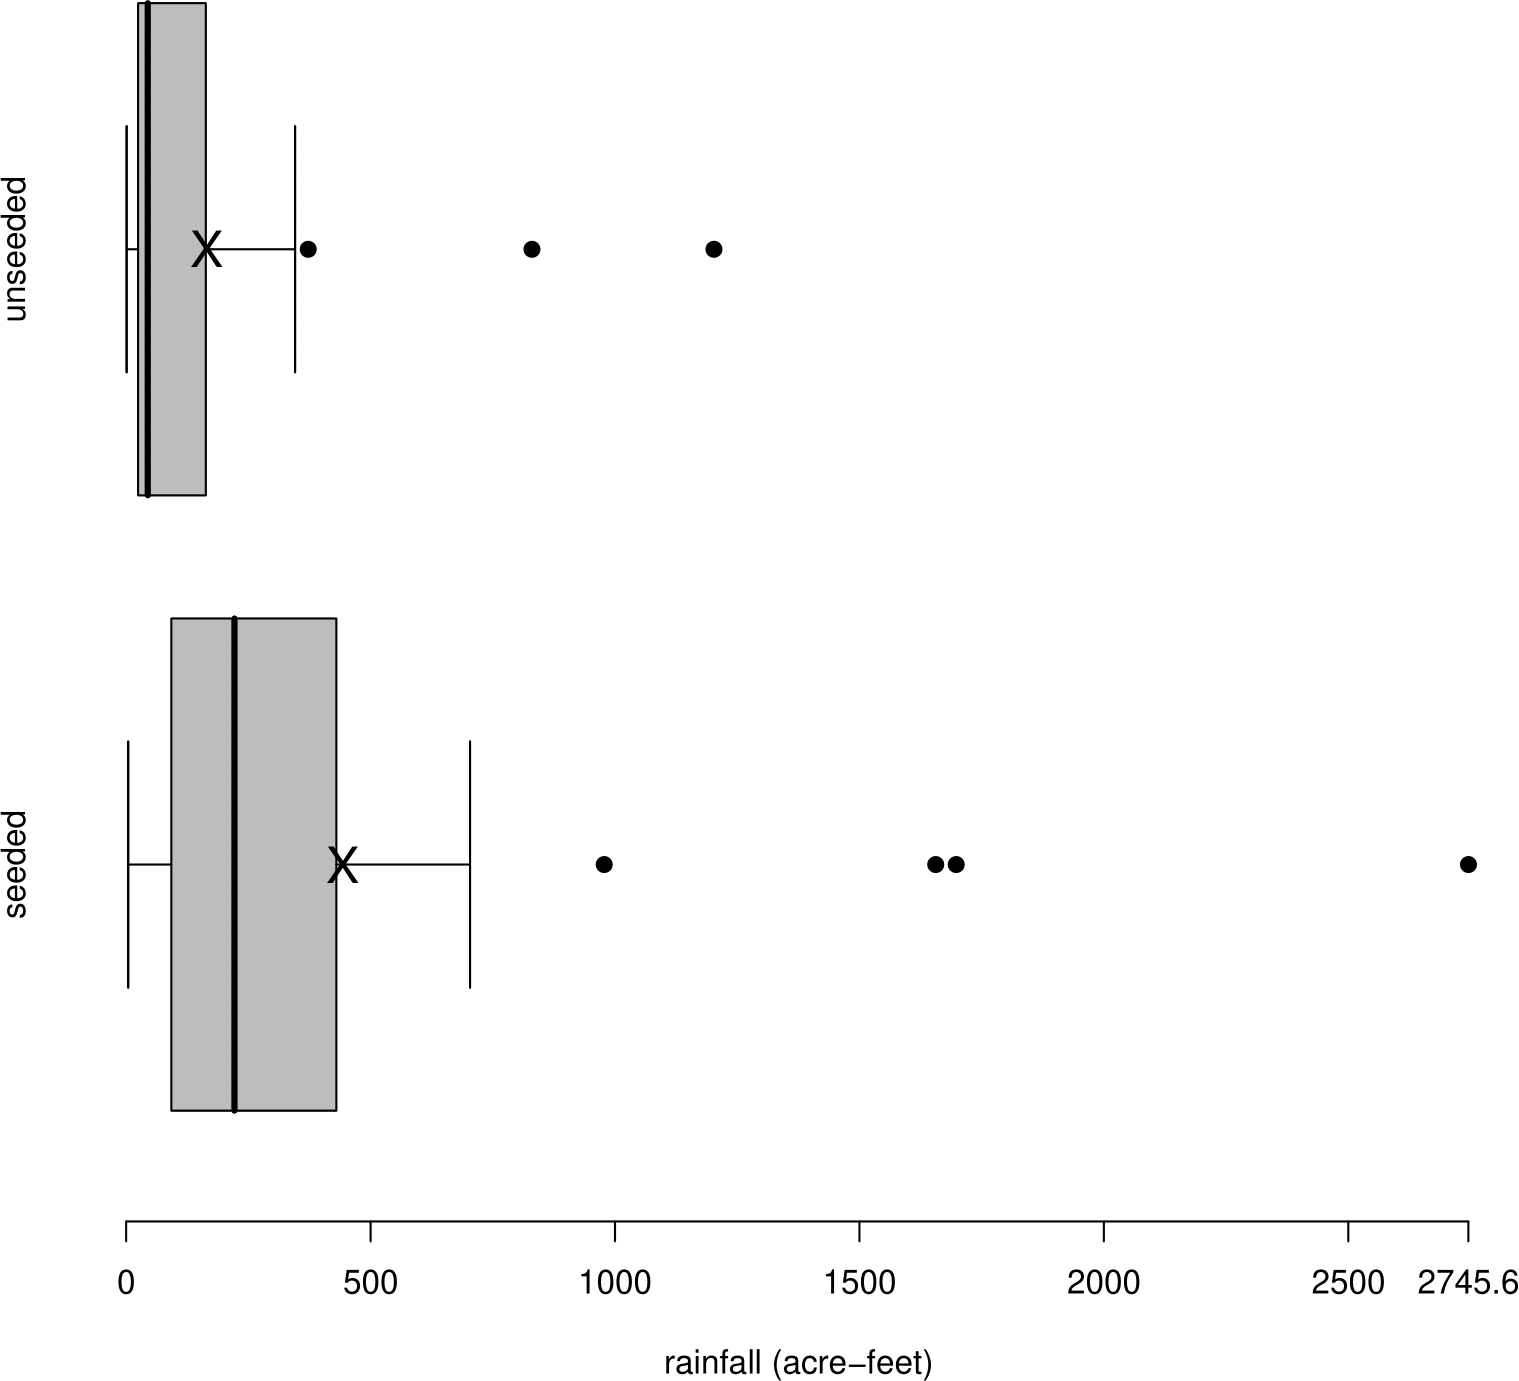
\includegraphics[width=0.75\linewidth]{images/cloud_box} 

}

\caption{Boxplots of rainfall in acre-feet for seeded and unseeded clouds.  Sample means are marked with a cross.}\label{fig:cloudbox}
\end{figure}

It is clear from the shape of these plots that the data are positively skewed. Also, the sample means are much greater than their corresponding sample medians. Measurements of (positive) environmental quantities are often positive skew. In addition, the rainfall values from the seeded clouds have a both higher location and a higher spread than the values from the unseeded clouds. After a log transformation (see \ref{fig:cloudboxlog}), the data are closer to being approximately symmetric. The sample means are closer to their corresponding sample medians. In addition the log transformation makes the variances of the rainfall values in the two groups more nearly equal.

\begin{figure}

{\centering 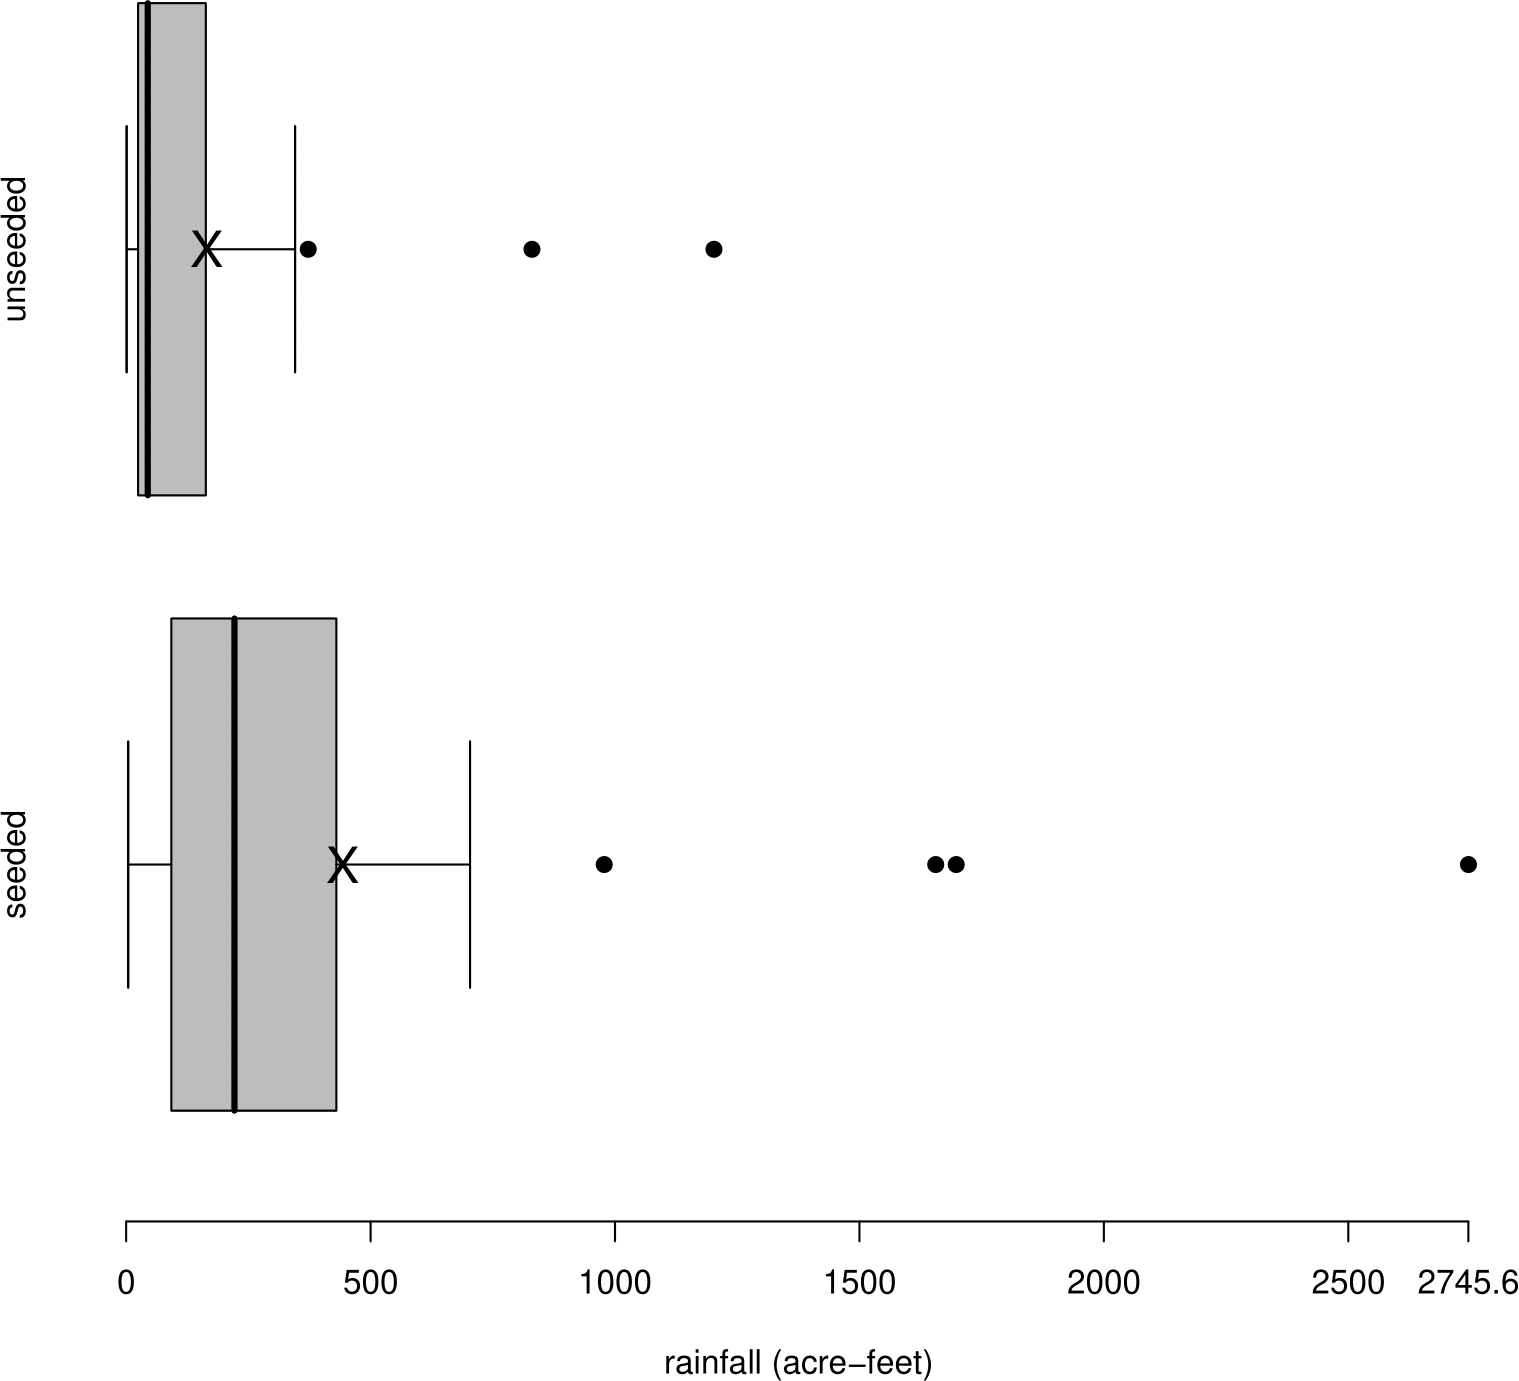
\includegraphics[width=0.75\linewidth]{images/cloud_box} 

}

\caption{Boxplots of rainfall in acre-feet for seeded and unseeded clouds after a $\log_{10}$ transformation has been applied.  Sample means are mared with a cross.}\label{fig:cloudboxlog}
\end{figure}

We have used a log transformation make positive skew data more symmetric. Other transformations which can be useful for this purpose are: \(y^c\), where \(c<1\), for example, \(\sqrt{y}\), \(1/y\). These transformations stretch out the lower tail. In contrast, \(y^c\), where \(c>1\), e.g.~\(y^2\), \(y^3\), may be used to transform negative skew data to approximate symmetry. These transformations stretch out the upper tail. It may seem that the log transformation is of an entirely different form to the other transformations, that is, \(y^c\) for some \(c \neq 0\). However, we will see that a log transformation can be obtained by considering the behaviour of the equivalent transformation \((y^c - 1) / c\) as \(c\) approaches zero.

It is possible to transform using \(y^c\) for \textbf{any} real value of \(c\), but it is better to stick to simple powers, such as the ones above, as it is more likely that these will have a sensible interpretation. The further \(c\) is from 1 the more difference the transformation makes.

These rainfall data are positive so there is no problem using a transformation of the form \(y^c\). However, if a dataset contains negative values then there are problems. If \(y<0\) then \(y^c\) can only be calculated in special cases where \(c\) is an integer. We also need to be able to invert the transformation, that is, to infer the value of \(y\) uniquely from the value of \(y^c\). If \(y\) can be both negative and positive then this is only possible in the very special cases where \(c\) is an odd integer. If a dataset contains zeros then we cannot use a log transformation, or \(y^c\) for \(c < 0\). The main point is that we need all the data to be positive in order to use the transformation \(y^c\) (or \((y^c - 1) / c\)). If we wish to transform data with non-positive values it is common to add a suitable constant to all values, to produce positive data, before transformation.

The rainfall data range over several orders of magnitude, that is, from one to well over a thousand. Applying a log transformation is often useful when data range over several orders of magnitude.

\textbf{An aside}. If we particularly like stem-and-leaf plots then we could produce a back-to-back stem-and-leaf plot, as in the plots of the log-transformed rainfall totals in Figure \ref{fig:cloudstem}.

\begin{figure}

{\centering 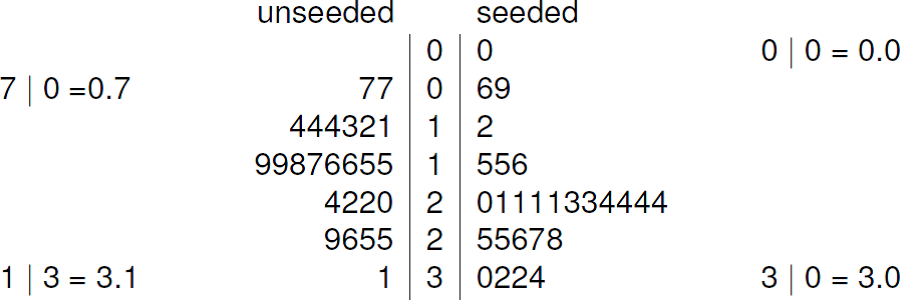
\includegraphics[width=0.75\linewidth]{images/cloud_stem} 

}

\caption{Back to back stem-and-leaf plot of $\log_{10}$(rainfall) for the cloud seeding data. The decimal point is at the vertical line |. Leaf unit = 0.1 log(acre feet)}\label{fig:cloudstem}
\end{figure}

\hypertarget{straighten}{%
\subsection{Straightening scatter plots}\label{straighten}}

Suppose we have drawn a scatter plot and the general form of the relationship between the variables \(y\) and \(x\) appears to be monotonic, \(y\) tends either to increase or decrease with the value of \(x\), subject to some random scatter about this relationships. However, the relationship between the variables \(y\) and \(x\) is not even approximately a straight line, that is, it is non-linear, rather than linear.

There are two main reasons why we may want to \textbf{straighten out} a scatter plot, that is, make it closer to being linear:

\begin{itemize}
\tightlist
\item
  we may be find it easier to appeciate the relationship between variables when that relationship is linear compared to a case where the relationship is non-linear and more complicated;
\item
  we may be hoping to be able to use a simple method of analysis that requires approximate linearity, for example, linear regression (see Chapter \ref{linreg}).
\end{itemize}

\hypertarget{how-can-we-straighten-a-scatter-plot}{%
\subsubsection*{How can we straighten a scatter plot?}\label{how-can-we-straighten-a-scatter-plot}}
\addcontentsline{toc}{subsubsection}{How can we straighten a scatter plot?}

We could transform the \(y\) variable, that is, plot a function of \(y\) on the \(y\)-axis. As in Section \ref{transsymmetry}, commonly-used transformations are

\[
y^3\,, \quad
y^2\,, \quad
(y)\,, \quad 
\sqrt{y}\,, \quad
\log y\,, \quad
-\frac{1}{\sqrt{y}}\,, \quad
-\frac1y\,, \quad
-\frac{1}{y^2}\,, \quad
-\frac{1}{y^3}\,, \quad 
\]

\textbf{Question}: Why might we prefer to use the transformation \(-1/y\), rather than \(1/y\)?

Instead of transforming the \(y\)-axis we could transform the \(x\) variable, or both the \(y\) and \(x\) variables. For example, in Figure \ref{fig:scatter1b} the use of a square root transformation on \(y\) and a log transformation on \(x\) produces a plot in which the relationship between the two variables is much closer being approximately linear than the variables plotted in Figure \ref{fig:scatter1a}.

If we wish to use transformation to straighten a scatter plot then we have lots of choice about which transformations to try. These days it is easy to use trial-and-error, that is, to try lots of transformations and judge by eye which of the resulting plots we prefer. There are also automatic computational methods to do this. However, before the advent of modern computing, producing plots was more time-consuming and it was helpful to use the shape of the original plot to suggest which transformations might work. One way to do this is sometimes called \textbf{Tukey and Mosteller's bulging rule}.

Consider the curve plotted in Figure \ref{fig:hollowup}. Imagine a straight line drawn between the ends of this curve. In the middle of the curve the values of both \(y\) and \(x\) are smaller than the points on the imaginary line. We say that the curve is bulging down in both the \(y\) and \(x\) directions.

\begin{figure}

{\centering 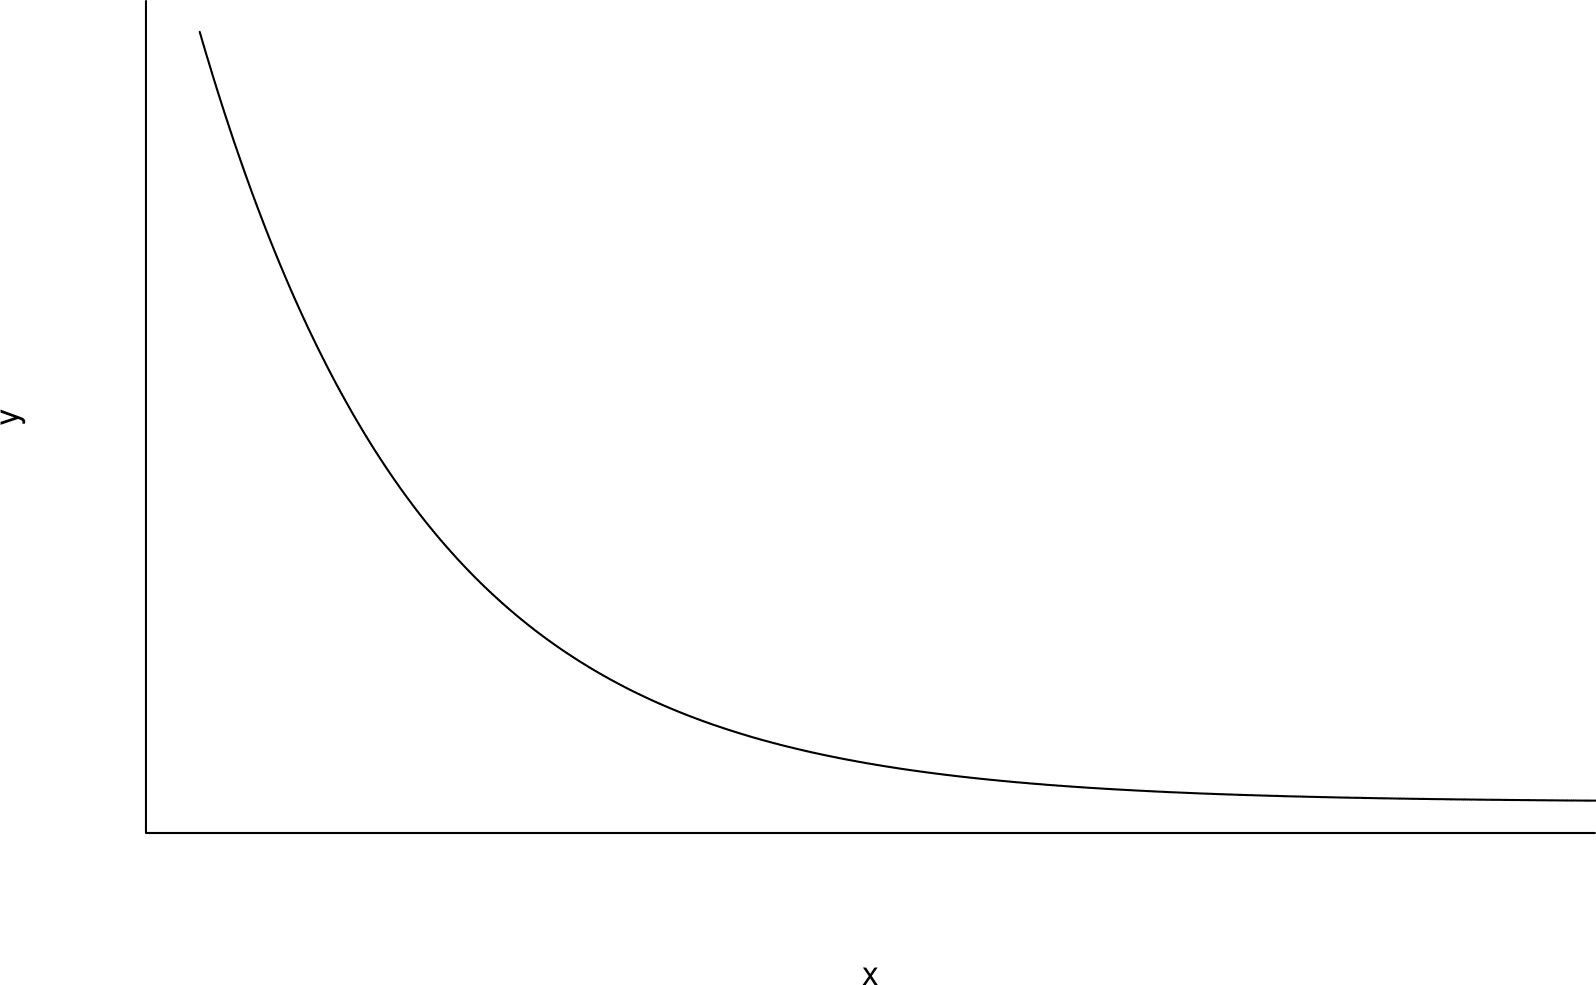
\includegraphics[width=0.75\linewidth]{images/hollow_up} 

}

\caption{A curve in which both $y$ and $x$ are bulging down compared to an imaginary straight line drawn between the ends of the curve.}\label{fig:hollowup}
\end{figure}

Similarly, in Figure \ref{fig:hollowdown} \(x\) is bulging down but now \(y\) is bulging up.

\begin{figure}

{\centering 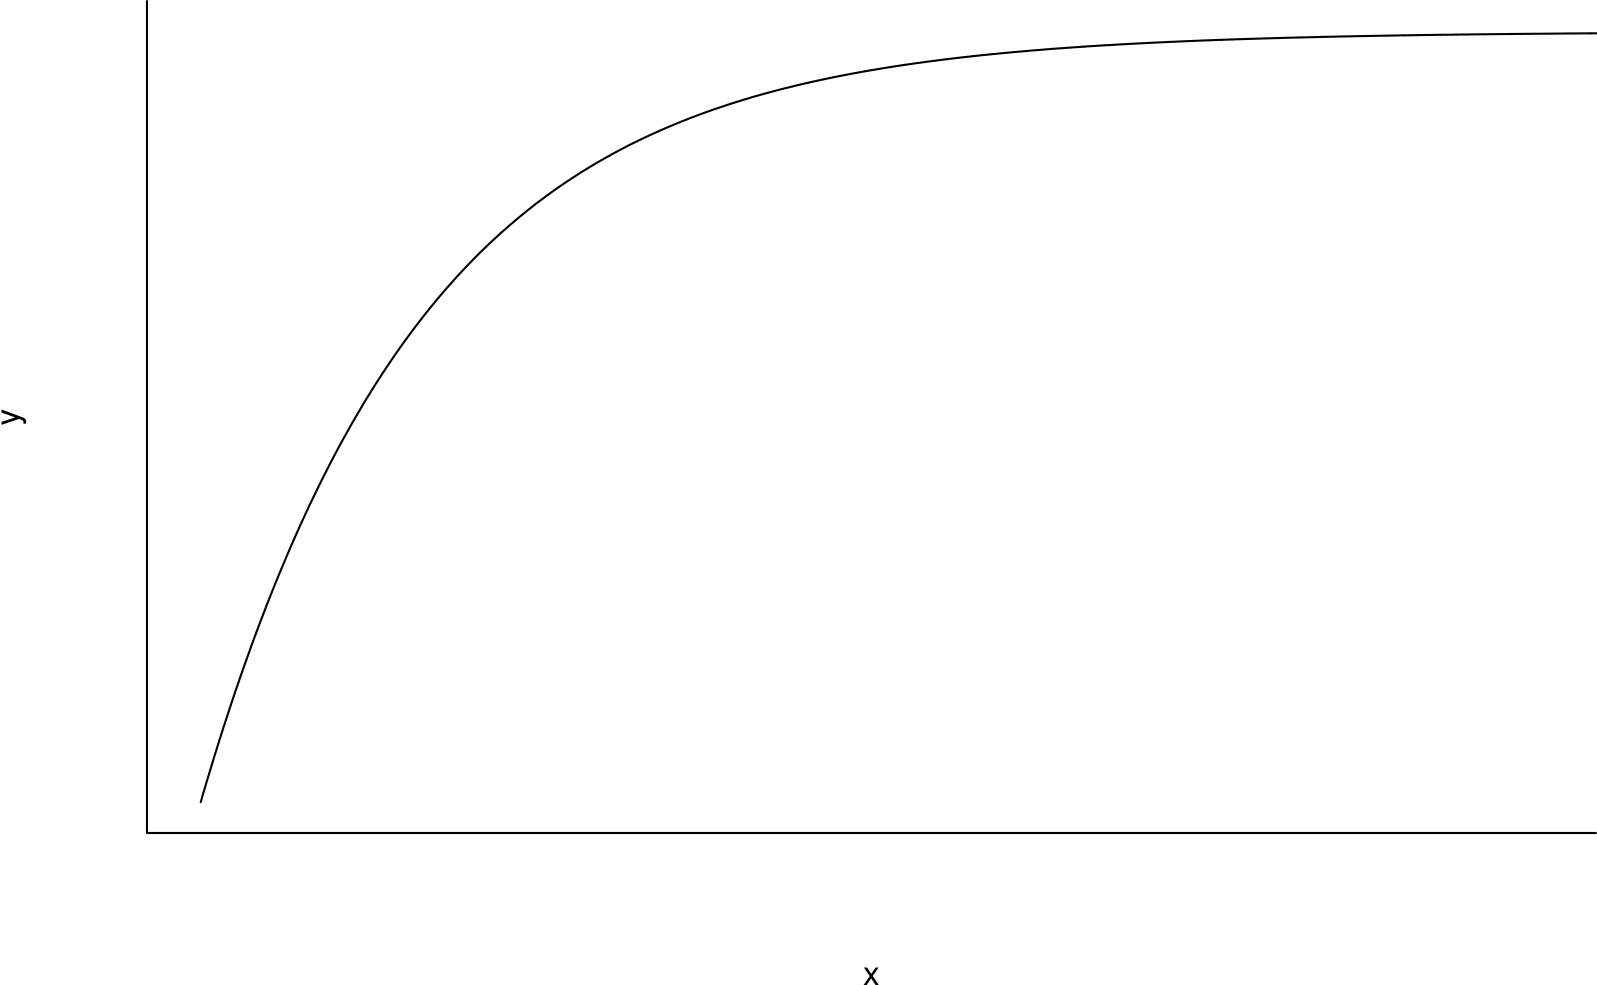
\includegraphics[width=0.75\linewidth]{images/hollow_down} 

}

\caption{A curve in which both $y$ and $x$ are bulging down compared to an imaginary straight line drawn between the ends of the curve.}\label{fig:hollowdown}
\end{figure}

Suppose that we consider transforming only \(y\). Tukey and Mosteller's bulging rule says that for scatter plots showing relationships like that depicted in Figure \ref{fig:hollowup} we should try transformations like \(\sqrt{y}, \, \log y, \,-1/\sqrt{y}, \, -1/y, \, -1/y^2, \ldots\), that is, \(y^c\), for \(c < 1\). For cases like Figure \ref{fig:hollowup} we should try transformations like \(y^2, \, y^3, \ldots\), that is, \(y^c\), for \(c > 1\).

Consider Figure \ref{fig:electionHS1} as an example. The relationship between the variables is similar to the curve in Figure \ref{fig:hollowup}. Therefore, we should try transforming \(y\) using using a transformation like \(\sqrt{y}, \, \log y, \ldots\).

\begin{figure}

{\centering 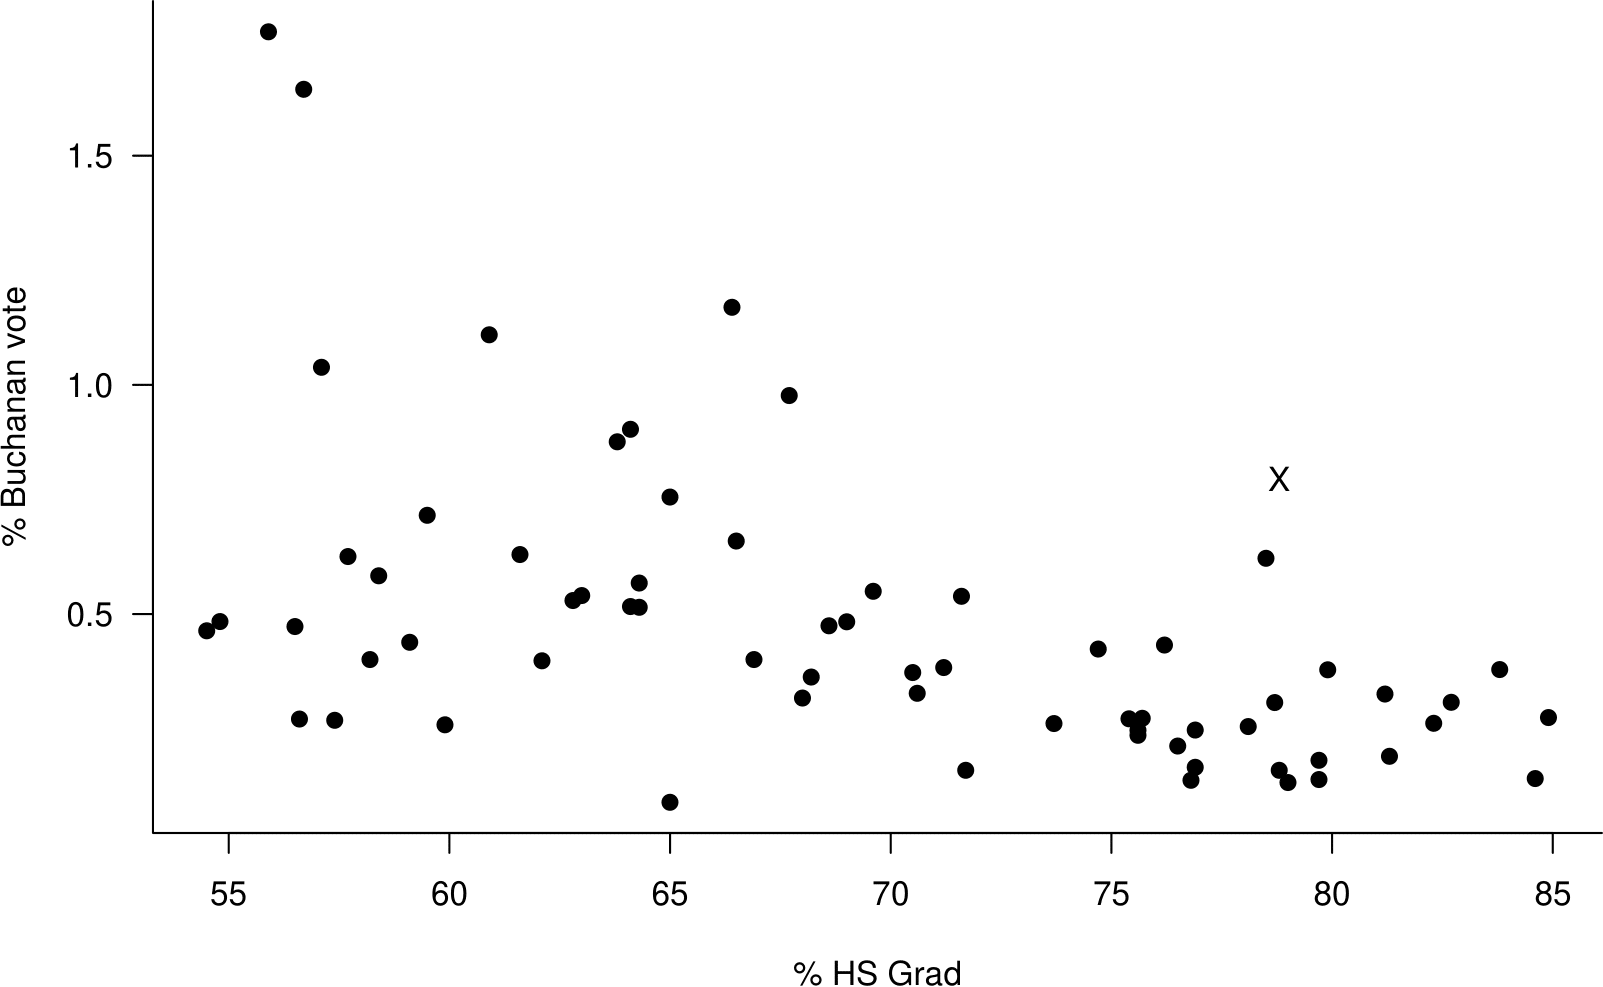
\includegraphics[width=0.75\linewidth]{images/election_HS1} 

}

\caption{Scatter plot of the percentage of the vote obtained by Buchanan against the percentage of the population who graduate from high school the 2000 US Presidential Election data.}\label{fig:electionHS1}
\end{figure}

The curvature of the relationship shown in \ref{fig:electionHS1} is not strong, so it makes sense that in Figure \ref{fig:electionHS2} approximately linearity of relationship is acheived using the relatively weak transformation \(\sqrt{y}\).

\begin{figure}

{\centering 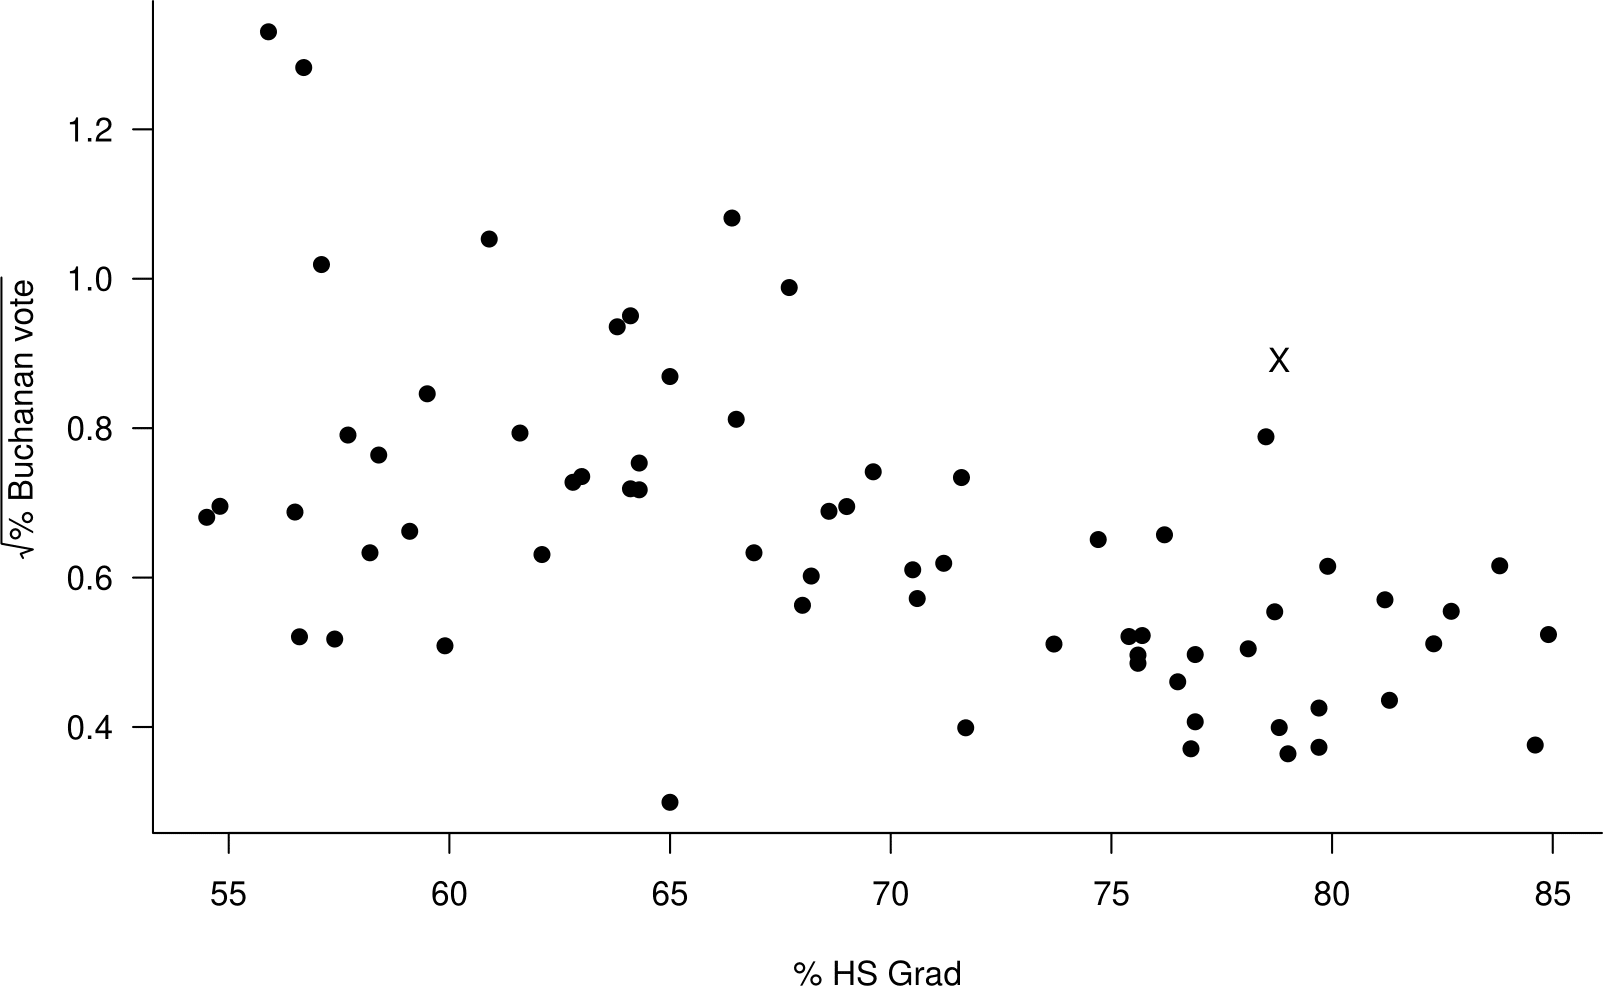
\includegraphics[width=0.75\linewidth]{images/election_HS2} 

}

\caption{Scatter plot of the square root of the percentage of the vote obtained by Buchanan against the percentage of the population who graduate from high school the 2000 US Presidential Election data.}\label{fig:electionHS2}
\end{figure}

Figure \ref{fig:tukey} shows how Tukey and Mosteller's bulging rule works in the four different bulging cases, considering the possibilities of transforming \(y\) only, \(x\) only or both \(y\) and \(x\). To use this figure first pick the curve that is relevant to the scatter plot in question. The expressions given at the ends of this curve are examples of the kind of transformations that you could try. The general forms of the indicated transformations are given in the caption to the figure.

\begin{figure}

{\centering 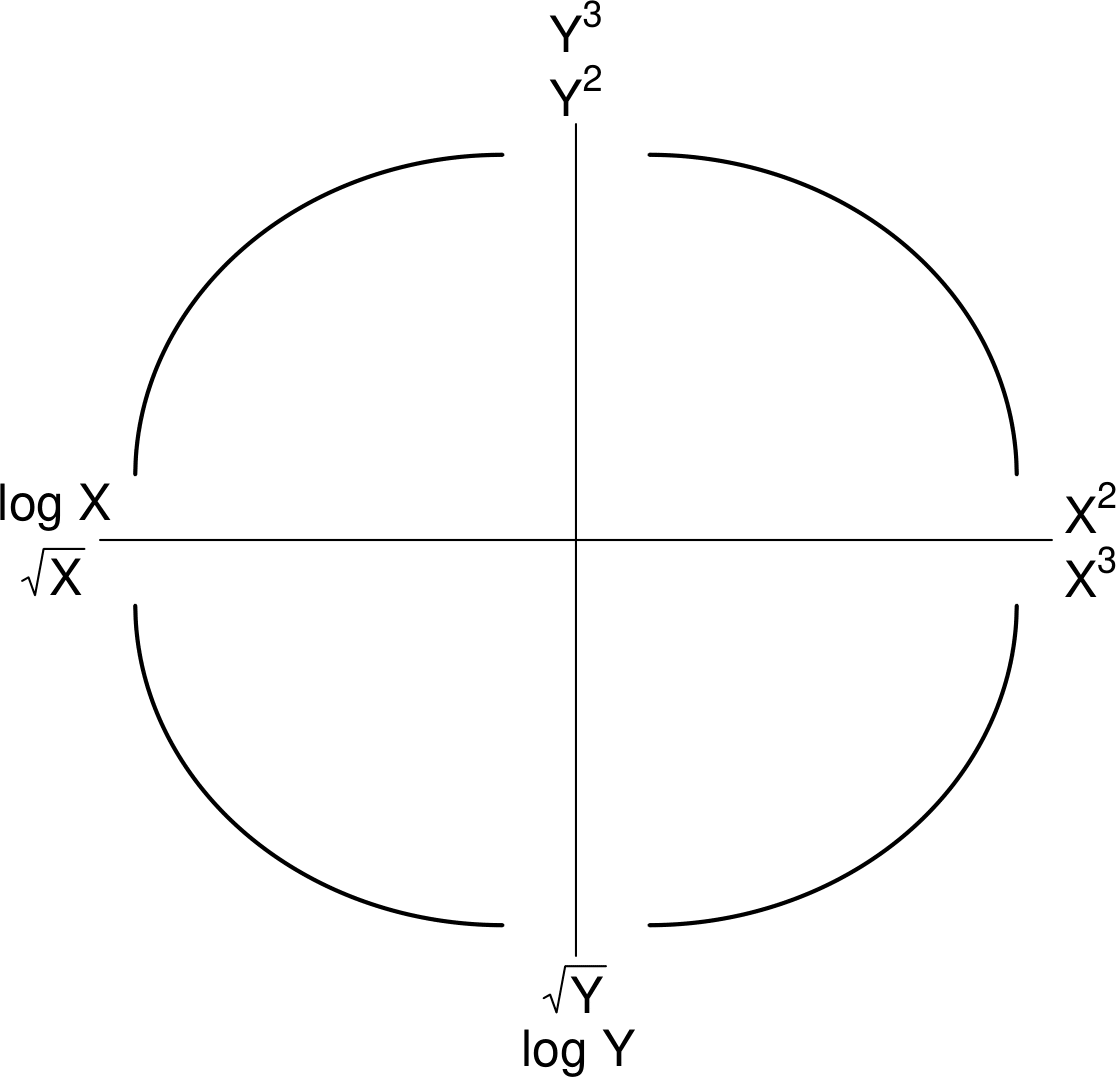
\includegraphics[width=0.75\linewidth]{images/tukey} 

}

\caption{Summary of transformations, of the form $Y^{c_y}$ and/or $X^{c_x}$, to try. Bottom left: $c_y < 1, c_x < 1$. Top left: $c_y > 1, c_x < 1$.Top right: $c_y > 1, c_x > 1$.Bottom right: $c_y < 1, c_x > 1$.}\label{fig:tukey}
\end{figure}

\hypertarget{linearity-is-not-the-only-consideration}{%
\subsubsection*{Linearity is not the only consideration}\label{linearity-is-not-the-only-consideration}}
\addcontentsline{toc}{subsubsection}{Linearity is not the only consideration}

Although linearity can be important other things can be important too. Suppose that we draw a `line-of-best-fit' on a scatter plot which looks approximately linear. Figure \ref{fig:electionHS3} is a copy of Figure \ref{fig:electionHS2} with such a line superimposed. In Chapter \ref{linreg} we will see that in a simple linear regression model it is assumed that the amount of (vertical) scatter in the \(y\) direction of points about a line of best fit is the same for all values of the explanatory variable \(x\).

In Figure \ref{fig:electionHS3} there is perhaps a greater spread of points about the line for small values of \% HS Grad than for large values of \% HS Grad.

\begin{figure}

{\centering 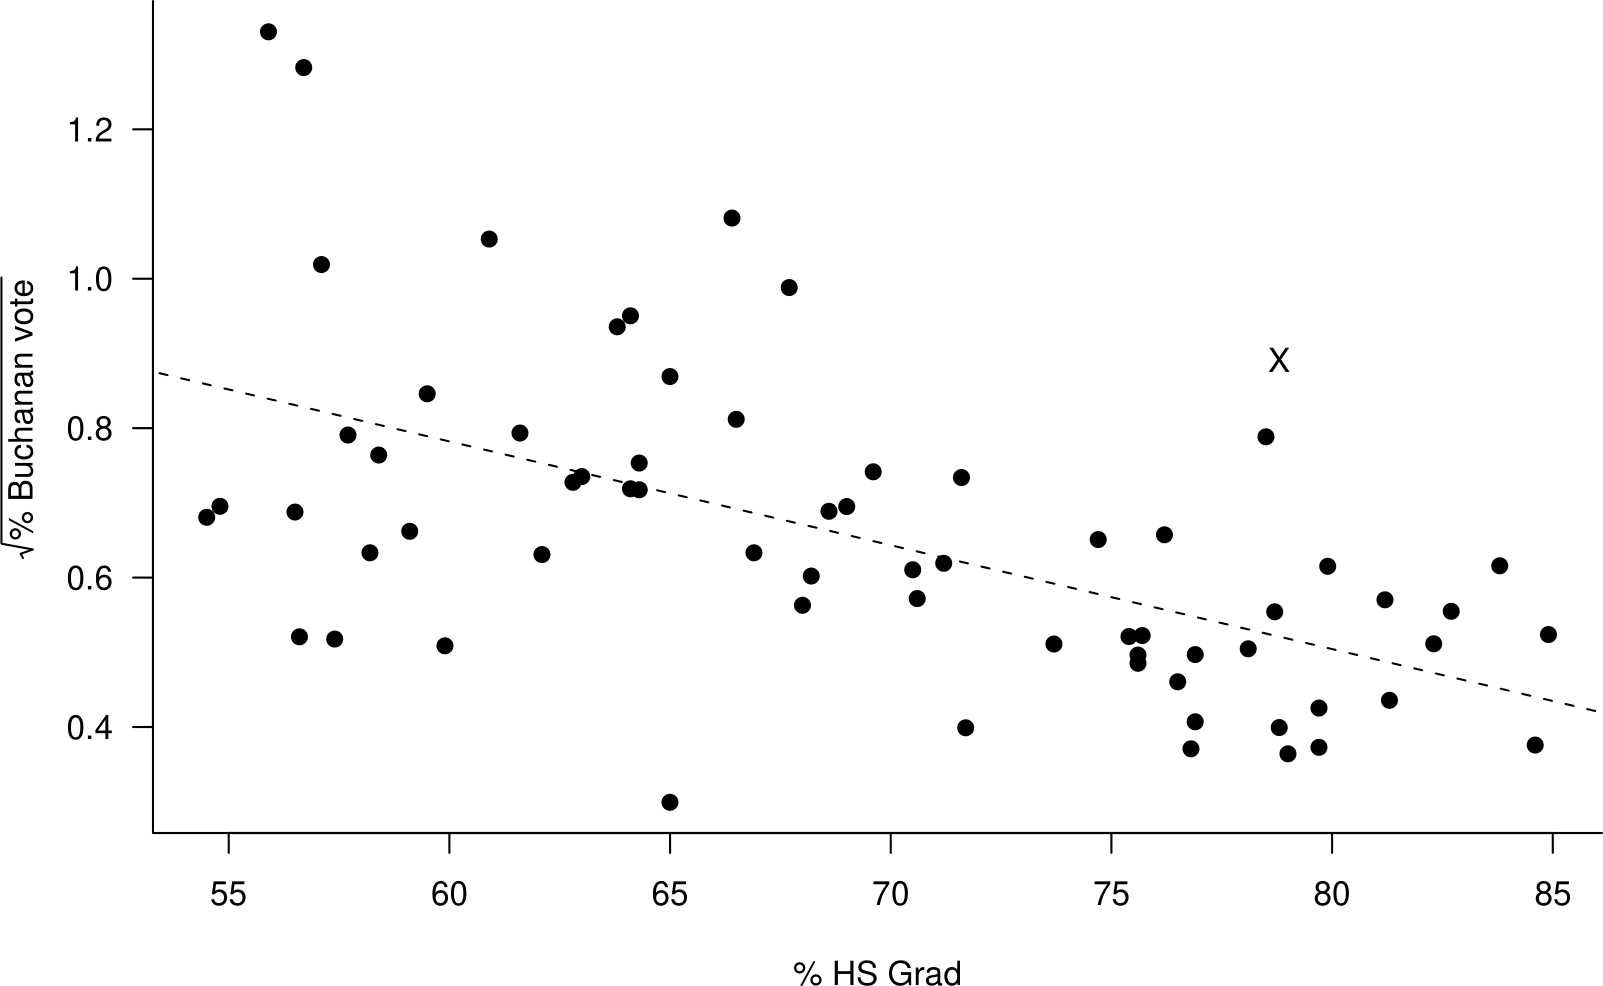
\includegraphics[width=0.75\linewidth]{images/election_HS3} 

}

\caption{Scatter plot of the square root of the percentage of the vote obtained by Buchanan against the percentage of the population who graduate from high school the 2000 US Presidential Election data.  A (dashed) line-of-best-fit is superimposed.}\label{fig:electionHS3}
\end{figure}

In Section \ref{linregtrans} we consider how to use transformation of \(y\) and/or \(x\) to satisfy better the assumptions of a linear regression model.

\hypertarget{probability}{%
\chapter{Probability}\label{probability}}

Most people have heard the word \textbf{probability} used in connection with a random experiment, that is, an experiment whose outcome cannot be predicted with certainty, such as tossing a coin, tossing dice, dealing cards etc. We start by considering a criminal case in which fundamental ideas surrounding the use of probability were hugely important. Then we study the concept of probability using the traditional simple example of tossing a coin.

\hypertarget{sids}{%
\section{Misleading statistical evidence in cot death trials}\label{sids}}

In recent years there have been three high-profile criminal cases in which a mother has been put on trial for the murder of a her babies. In each case the medical evidence against the woman was weak and the prosecution relied heavily on statistical arguments to make their case. However, these arguments were not made by a statistician, but by a medical expert witness: Professor Sir Roy Meadows. However, there were two problems with Professor Meadows' evidence: firstly, it contained serious statistical errors; and secondly, it was presented in a way which is likely to be misinterpreted by a jury. To illustrate the error we consider the case of Sally Clark.

Sally Clark's first child died unexpectedly in 1996 at the age of 3 months. Sally was the only person in the house at the time. There was evidence of a respiratory infection and the death was recorded as natural; a case of \textbf{Sudden Infant Death Syndrome (SIDS)}, or \textbf{cot death}. In 1998 Sally's second child died in similar circumstances at the age of 2 months. Sally was then charged with the murder of both babies. There was some medical evidence to suggest that the second baby could have been smothered, although this could be explained by an attempt at resuscitation.

It appeared that the decision to charge Sally was based partly on the reasoning that cot death is quite rare so having two cot deaths in the same family must be very unlikely indeed. This is the basis of Professor Meadows' assertion that: ``One cot death is a tragedy, two cot deaths is suspicious and, until the contrary is proved, three cot deaths is murder.''. At her trial in 1999 Sally Clark was found guilty of murder and sentenced to life imprisonment.

\hypertarget{professor-meadows-statistical-evidence}{%
\subsubsection*{Professor Meadows' statistical evidence}\label{professor-meadows-statistical-evidence}}
\addcontentsline{toc}{subsubsection}{Professor Meadows' statistical evidence}

At Sally Clark's trial in 1999 Professor Meadows claimed that, in a family like Sally's (affluent, non-smoking with a mother aged over 26), the chance of two cot deaths is 1 in 73 million, that is, a probability of 1/73,000,000 \(\approx\) 0.000000014. Professor Meadows had calculated this value based on a study which had estimated the probability of one cot death in a family like Sally's to be 1 in 8543, that is, 1 cot death occurs for every 8543 of such families.

Professor Meadows had then performed the calculation
\[\frac{1}{8543}\times\frac{1}{8543}=\frac{1}{72,982,849}\approx\frac{1}{73,000,000}.\]

There are problems with this evidence, both with this calculation and with the idea that this apparently small number provides evidence of guilt.

Can you identify these problems?

\hypertarget{relative-frequency-definition-of-probability}{%
\section{Relative frequency definition of probability}\label{relative-frequency-definition-of-probability}}

\hypertarget{example-tossing-a-coin}{%
\subsubsection*{Example: tossing a coin}\label{example-tossing-a-coin}}
\addcontentsline{toc}{subsubsection}{Example: tossing a coin}

If you toss a coin, the outcome (the side on top when the coin falls to the ground) is either a Head (\(H\)) or a Tail (\(T\)). Suppose that you toss the coin a large number of times. Unless you are very skillful the outcome of each toss depends on chance. Therefore, if you toss the coin repeatedly, the exact sequence of \(H\)s and \(T\)s is not predictable with certainty in advance. This is usually the case with any experiment. Even if we try very hard to repeat an experiment under exactly the same conditions, there is a certain amount of variability in the results which we cannot explain, but we must accept. The experiment is a
\textbf{random experiment}.

Nevertheless, if the coin is fair (equally balanced), and it is tossed fairly, we might expect the long run \textbf{proportion}, or \textbf{relative frequency}, of \(H\)s to settle down to 1/2. However, the only way to find out whether this is true is to toss a coin repeatedly, forever, and calculate the proportion of tosses on which \(H\) is the outcome. It is not possible, in practice, for any experiment to be repeated forever.

However, a South African statistician Jon Kerrich managed to toss a coin
10,000 times while imprisoned in Denmark during World War II. At the end of his
effort he had recorded 5067 Heads and 4933 Tails. Figure \ref{fig:coin} shows
how the proportion of heads Kerrich threw changed as the number of tosses increased.

\begin{figure}

{\centering 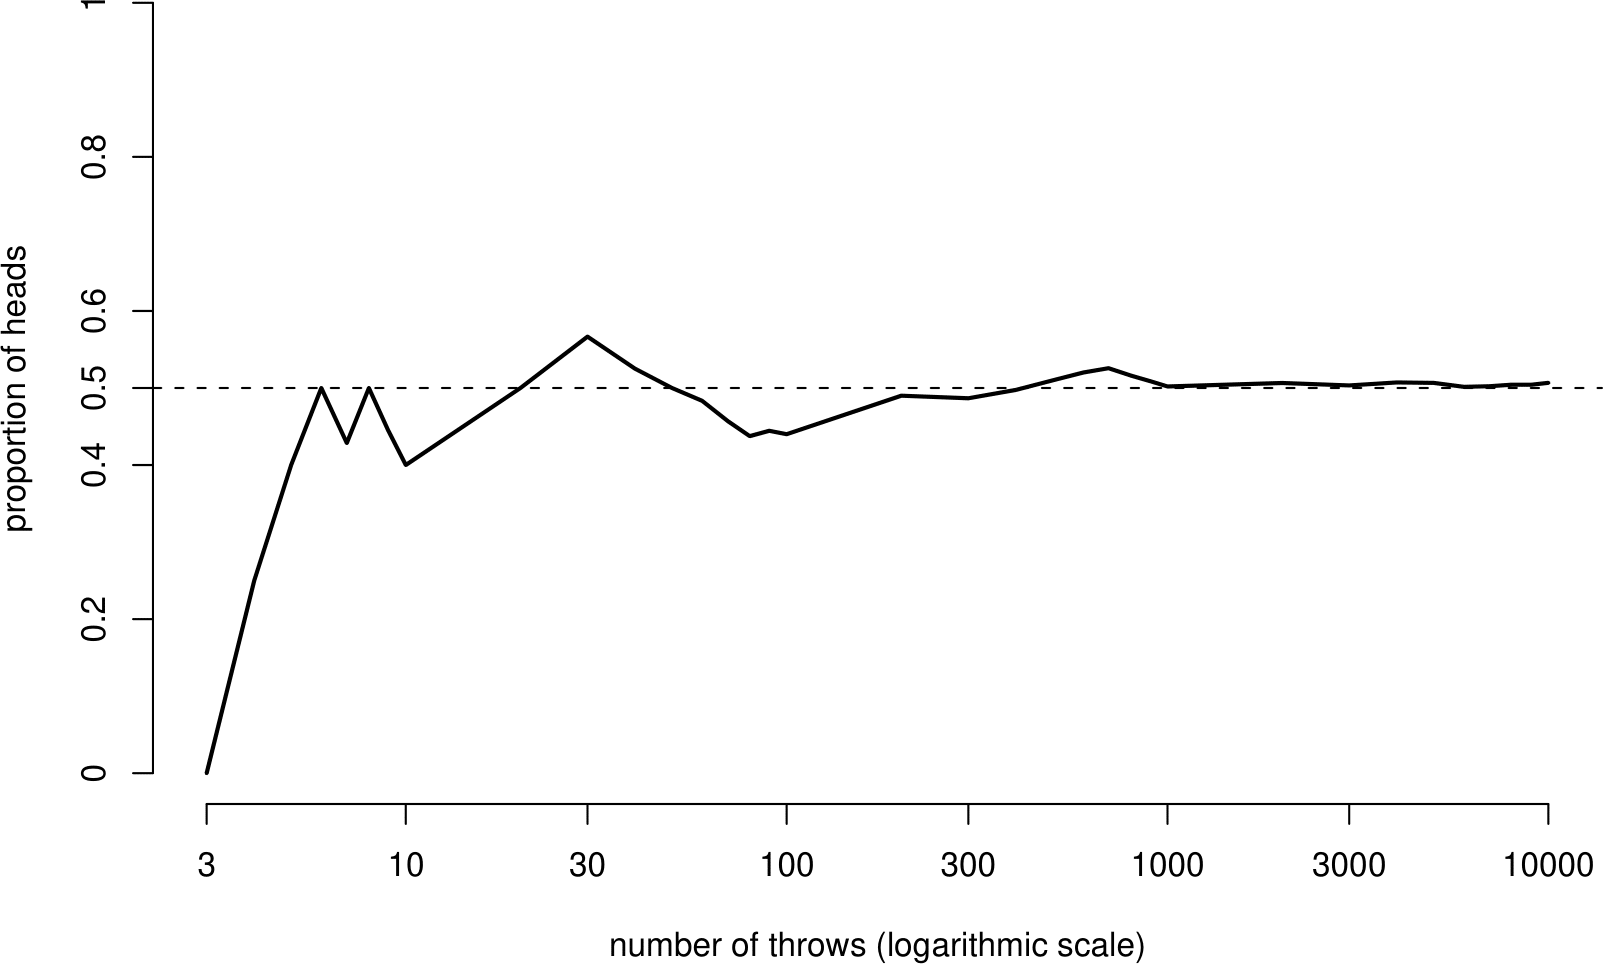
\includegraphics[width=0.75\linewidth]{images/coin} 

}

\caption{The proportion of heads in a sequence of 10,000 coin tosses. @coin.}\label{fig:coin}
\end{figure}

Initially the proportion of heads fluctuates greatly but begins to settle down as the number of tosses increases. After 10,000 tosses the relative frequency of Head is 5067/10,000=0.5067. We might suppose that if Kerrich were able to continue his experiment forever, the proportion of heads would tend to a limiting value which would be very near, if not exactly, 1/2. This hypothetical limiting value is the probability of heads and is denoted by \(P(H)\).

\hypertarget{looking-at-this-slightly-more-formally}{%
\subsubsection*{Looking at this slightly more formally}\label{looking-at-this-slightly-more-formally}}
\addcontentsline{toc}{subsubsection}{Looking at this slightly more formally}

The coin-tossing example motivates the \textbf{relative frequency} or \textbf{frequentist} definition of the probability of an event; namely

\begin{quote}
the relative frequency with which the event occurs in the long run;
\end{quote}

or, in other words,

\begin{quote}
the proportion of times that the event would occur in an infinite number of identical repeated experiments.
\end{quote}

Suppose that we toss a coin \(n\) times. If the coin is fair, and is tossed fairly, then it is reasonable to suppose that
\[\mbox{the relative frequency of $H$} \,\,=\,\, 
\frac{\mbox{number of times $H$ occurs}}{n},\]
tends to 1/2 as \(n\) gets larger. We say that the event \(H\) has probability 1/2, or \(P(H)=1/2\).

More generally, consider some event \(E\) based on the outcomes of an experiment. Suppose that the experiment can, in principle, be repeated, under exactly the same conditions, forever. Let \(n(E)\) denote the number of times that the event \(E\) would occur in \(n\) experiments.

We suppose that
\[\mbox{the relative frequency of $E$} \,=\,
\frac{n(E)}{n} \,\longrightarrow\, P(E)\,, \,\, \mbox{as }n \longrightarrow \infty.\]
So, the probability \(P(E)\) of the event \(E\) is defined as the limiting value of \(n(E)/n\) as \(n \rightarrow \infty\). That is,
\begin{equation}
P(E) \,\,=\,\, \mathop {\mathrm{limit}}\limits_{n \rightarrow \infty}\,\frac{n(E)}{n},
\label{eq:limit}
\end{equation}
supposing that this limit exists. (Note: I have written `limit' and not `lim' because this is not a limit in the usual mathematical sense.)

In order to satisfy ourselves that the probability of an event \textbf{exists}, we do not need to repeat an experiment an infinite number of times, or even be able to. All we need to do is \textbf{imagine} the experiment being performed repeatedly. An event with probability 0.75, say, would be expected to occur 75 times out of 100 in the long run.

An alternative approach, considered in STAT0003, makes a simple set of basic assumptions about probability, called the \textbf{axioms of probability}. Using these axioms it can be proved that the limiting relative frequency in equation \eqref{eq:limit} does exist and that it is equal to \(P(E)\). In STAT0002 we will not consider these axioms formally. However, they are so basic and intuitive that you will find that we take them for granted.

\textbf{An aside}. There is another definition of probability, the \textbf{subjective} definition, which is the degree of belief someone has in the occurrence of an event, based on their knowledge and any evidence they have already seen. For example, you might reasonably believe that the probability that a coin comes up Heads when it is tossed is 1/2 because the coin looks symmetrical. If you are \textbf{certain} that \(P(H)=1/2\) then no amount of evidence from actually tossing the coin will change your mind. However, if you just think that \(P(H)=1/2\) is more likely that other values of \(P(H)\) then observing many more \(H\)s than \(T\)s in a long sequence of tosses may lead you to believe that \(P(H)>1/2\). We will not consider this definition of probability again in this course. However, it forms the basis of the \textbf{Bayesian} approach to Statistics. You may study this in a more advanced courses, for example, STAT0008 Statistical Inference.

\hypertarget{example-tossing-a-coin-continued}{%
\subsubsection*{Example: tossing a coin (continued)}\label{example-tossing-a-coin-continued}}
\addcontentsline{toc}{subsubsection}{Example: tossing a coin (continued)}

We now look at the coin-tossing example in a slightly different way. If we toss a coin forever we generate an infinite \textbf{population} of \textbf{outcomes}: \{H,H,T,H,\ldots \}, say. Think about choosing, or \textbf{sampling}, one of these outcomes at random from this population. The probability that this outcome is \(H\) is the proportion of \(H\)s in the population. If we \textbf{assume} that the coin is fair then the infinite population contains 50\% \(H\)s and 50\% \(T\)s. In that case \(P(H)=1/2\), and \(P(T)=1/2\).

\hypertarget{example-graduate-admissioins-at-berkeley}{%
\subsubsection*{Example: Graduate Admissioins at Berkeley}\label{example-graduate-admissioins-at-berkeley}}
\addcontentsline{toc}{subsubsection}{Example: Graduate Admissioins at Berkeley}

Table \ref{tab:berk0} contains data relating to graduate admissions in 1973 at the University of California, Berkeley, USA in the six largest (in terms of numbers of admissions) departments of the university. These data are discussed in \citet{berkeley}. We use the following notation: \(A\) for an accepted applicant, \(R\) for a rejected applicant. Table \ref{tab:berk0n} summarises the notation used for the frequencies in Table \ref{tab:berk0}. For example, \(n(A)\) denotes the number of applicants who were accepted. We will look at this example in more detail later.

 
  \providecommand{\huxb}[2]{\arrayrulecolor[RGB]{#1}\global\arrayrulewidth=#2pt}
  \providecommand{\huxvb}[2]{\color[RGB]{#1}\vrule width #2pt}
  \providecommand{\huxtpad}[1]{\rule{0pt}{#1}}
  \providecommand{\huxbpad}[1]{\rule[-#1]{0pt}{#1}}

\begin{table}[ht]
\begin{centerbox}
\begin{threeparttable}
\captionsetup{justification=centering,singlelinecheck=off}
\caption{\label{tab:berk0} Numbers of graduate applicants by outcome.}
 \setlength{\tabcolsep}{0pt}
\begin{tabularx}{0.6\textwidth}{p{0.2\textwidth} p{0.2\textwidth} p{0.2\textwidth}}


\hhline{>{\huxb{255, 255, 255}{0.1}}->{\huxb{255, 255, 255}{0.1}}->{\huxb{255, 255, 255}{0.1}}-}
\arrayrulecolor{black}

\multicolumn{1}{!{\huxvb{0, 0, 0}{0}}p{0.2\textwidth}!{\huxvb{0, 0, 0}{1}}}{\cellcolor[RGB]{255, 255, 255}\hspace{6pt}\parbox[b]{0.2\textwidth-6pt-6pt}{\huxtpad{6pt + 1em}\centering \textit{A}\huxbpad{6pt}}} &
\multicolumn{1}{p{0.2\textwidth}!{\huxvb{0, 0, 0}{1}}}{\cellcolor[RGB]{255, 255, 255}\hspace{6pt}\parbox[b]{0.2\textwidth-6pt-6pt}{\huxtpad{6pt + 1em}\centering \textit{R}\huxbpad{6pt}}} &
\multicolumn{1}{p{0.2\textwidth}!{\huxvb{0, 0, 0}{0}}}{\cellcolor[RGB]{255, 255, 255}\hspace{6pt}\parbox[b]{0.2\textwidth-6pt-6pt}{\huxtpad{6pt + 1em}\centering total\huxbpad{6pt}}} \tabularnewline[-0.5pt]


\hhline{>{\huxb{0, 0, 0}{1}}->{\huxb{0, 0, 0}{1}}->{\huxb{0, 0, 0}{1}}-}
\arrayrulecolor{black}

\multicolumn{1}{!{\huxvb{0, 0, 0}{0}}p{0.2\textwidth}!{\huxvb{0, 0, 0}{1}}}{\cellcolor[RGB]{255, 255, 255}\hspace{6pt}\parbox[b]{0.2\textwidth-6pt-6pt}{\huxtpad{6pt + 1em}\centering 1755\huxbpad{6pt}}} &
\multicolumn{1}{p{0.2\textwidth}!{\huxvb{0, 0, 0}{1}}}{\cellcolor[RGB]{255, 255, 255}\hspace{6pt}\parbox[b]{0.2\textwidth-6pt-6pt}{\huxtpad{6pt + 1em}\centering 2771\huxbpad{6pt}}} &
\multicolumn{1}{p{0.2\textwidth}!{\huxvb{0, 0, 0}{0}}}{\cellcolor[RGB]{255, 255, 255}\hspace{6pt}\parbox[b]{0.2\textwidth-6pt-6pt}{\huxtpad{6pt + 1em}\centering 4526\huxbpad{6pt}}} \tabularnewline[-0.5pt]


\hhline{>{\huxb{0, 0, 0}{1}}|>{\huxb{0, 0, 0}{1}}|}
\arrayrulecolor{black}
\end{tabularx}
\end{threeparttable}\par\end{centerbox}

\end{table}
 



 
  \providecommand{\huxb}[2]{\arrayrulecolor[RGB]{#1}\global\arrayrulewidth=#2pt}
  \providecommand{\huxvb}[2]{\color[RGB]{#1}\vrule width #2pt}
  \providecommand{\huxtpad}[1]{\rule{0pt}{#1}}
  \providecommand{\huxbpad}[1]{\rule[-#1]{0pt}{#1}}

\begin{table}[ht]
\begin{centerbox}
\begin{threeparttable}
\captionsetup{justification=centering,singlelinecheck=off}
\caption{\label{tab:berk0n} Notation for Table \ref{tab:berk0}.}
 \setlength{\tabcolsep}{0pt}
\begin{tabularx}{0.6\textwidth}{p{0.2\textwidth} p{0.2\textwidth} p{0.2\textwidth}}


\hhline{>{\huxb{255, 255, 255}{0.1}}->{\huxb{255, 255, 255}{0.1}}->{\huxb{255, 255, 255}{0.1}}-}
\arrayrulecolor{black}

\multicolumn{1}{!{\huxvb{0, 0, 0}{0}}p{0.2\textwidth}!{\huxvb{0, 0, 0}{1}}}{\cellcolor[RGB]{255, 255, 255}\hspace{6pt}\parbox[b]{0.2\textwidth-6pt-6pt}{\huxtpad{6pt + 1em}\centering \textit{A}\huxbpad{6pt}}} &
\multicolumn{1}{p{0.2\textwidth}!{\huxvb{0, 0, 0}{1}}}{\cellcolor[RGB]{255, 255, 255}\hspace{6pt}\parbox[b]{0.2\textwidth-6pt-6pt}{\huxtpad{6pt + 1em}\centering \textit{R}\huxbpad{6pt}}} &
\multicolumn{1}{p{0.2\textwidth}!{\huxvb{0, 0, 0}{0}}}{\cellcolor[RGB]{255, 255, 255}\hspace{6pt}\parbox[b]{0.2\textwidth-6pt-6pt}{\huxtpad{6pt + 1em}\centering total\huxbpad{6pt}}} \tabularnewline[-0.5pt]


\hhline{>{\huxb{0, 0, 0}{1}}->{\huxb{0, 0, 0}{1}}->{\huxb{0, 0, 0}{1}}-}
\arrayrulecolor{black}

\multicolumn{1}{!{\huxvb{0, 0, 0}{0}}p{0.2\textwidth}!{\huxvb{0, 0, 0}{1}}}{\cellcolor[RGB]{255, 255, 255}\hspace{6pt}\parbox[b]{0.2\textwidth-6pt-6pt}{\huxtpad{6pt + 1em}\centering \textit{n(A)}\huxbpad{6pt}}} &
\multicolumn{1}{p{0.2\textwidth}!{\huxvb{0, 0, 0}{1}}}{\cellcolor[RGB]{255, 255, 255}\hspace{6pt}\parbox[b]{0.2\textwidth-6pt-6pt}{\huxtpad{6pt + 1em}\centering \textit{n(R)}\huxbpad{6pt}}} &
\multicolumn{1}{p{0.2\textwidth}!{\huxvb{0, 0, 0}{0}}}{\cellcolor[RGB]{255, 255, 255}\hspace{6pt}\parbox[b]{0.2\textwidth-6pt-6pt}{\huxtpad{6pt + 1em}\centering \textit{n}\huxbpad{6pt}}} \tabularnewline[-0.5pt]


\hhline{>{\huxb{0, 0, 0}{1}}|>{\huxb{0, 0, 0}{1}}|}
\arrayrulecolor{black}
\end{tabularx}
\end{threeparttable}\par\end{centerbox}

\end{table}
 

The population of interest now is the population of graduate applicants to the six largest departments of the Berkeley. If we choose an applicant at random from this population the probability \(P(A)\) that they are accepted is given by
\[ P(A) = \frac{n(A)}{n} = \frac{1,755}{4,526} = 0.388.\]
Similarly, the probability \(P(R)\) that a randomly chosen applicant is rejected is given by
\[ P(R) = \frac{n(R)}{n} = \frac{2,771}{4,526} = 0.612.\]

In both the coin-tossing and Berkeley admissions examples we have imagined choosing an individual from a population in such a way that all individuals are equally likely to be chosen. The probability of the individual having a particular property, for example, that an applicant is accepted, is given by the proportion of individuals in the population which have this property.

In the coin-tossing example the population is hypothetical, generated by thinking about repeating an experiment an infinite number of times. In the Berkeley admissions example the population is an actual population of people.

\hypertarget{notation-sample-space-outcomes-and-events}{%
\subsubsection*{Notation: sample space, outcomes and events}\label{notation-sample-space-outcomes-and-events}}
\addcontentsline{toc}{subsubsection}{Notation: sample space, outcomes and events}

The set of all possible outcomes of a random experiment is called the \textbf{sample space} \(S\) of the experiment. We may denote a single \textbf{outcome} of an experiment by \(s\). An \textbf{event} \(E\) is a collection of outcomes, possible just one outcome.

It is very important to define the sample space \(S\) carefully. In the coin-tossing example we have \(S=\{H,T\}\). If the coin is unbiased then the probabilities of the outcomes in \(S\) are given by \(P(H)=1/2\) and \(P(T)=1/2\).

\hypertarget{basic-properties-of-probability}{%
\section{Basic properties of probability}\label{basic-properties-of-probability}}

Since we have defined probability as a proportion, basic properties of proportions must also hold for a probability. Consider an event \(E\). Then the following must hold

\begin{itemize}
\tightlist
\item
  \(0 \leq P(E) \leq 1\);
\item
  if \(E\) is impossible then \(P(E)=0\);
\item
  if \(E\) is certain then \(P(E)=1\);
\item
  \(P(S)=1\). This is true because the outcome must, by definition, be in the sample space.
\end{itemize}

\hypertarget{conditional-probability}{%
\section{Conditional probability}\label{conditional-probability}}

In Section \ref{sids} the statistical evidence presented to the court was based on the estimate that ``the probability of one cot death \textbf{in a family like Sally Clark's} is 1 in 8543''. What does this mean?

The study from which this statistic was taken estimated the \textbf{overall} probability of cot death to be 1 in 1303. That is, cot death occurs in approximately 1 in every 1303 families.

However, the study also found that the probability of cot death depended on various characteristics such as, income, smoking status and the age of the mother. For example, the probability of cot death was found to be much greater in families containing one or more smokers than in non-smoking families.

The study estimated the probability of cot death for each possible combination of these characteristics. For the combination which is relevant to Sally Clark, whose family was affluent, non-smoking and she was aged over 26, the probability of cot death was estimated to be smaller: 1 in 8543.

This (1 in 8543) is a \textbf{conditional} probability. We have \textbf{conditioned} on the event that the family in question is affluent, non-smoking and the mother is aged over 26. The overall probability of cot death (1 in 1303) is often called an \textbf{unconditional} probability.

In this example it is perhaps easiest to think of the conditioning as selecting a specific sub-population of families from the complete population of families. Another way to think about this is in terms of the sample space. We have reduced the original sample space - the outcomes (cot death or no cot death) of all families with children - to a subset of this sample space - the outcomes of all affluent, non-smoking families where the mother is over 26.

\hypertarget{notation}{%
\subsubsection*{Notation}\label{notation}}
\addcontentsline{toc}{subsubsection}{Notation}

When we are working with conditional probabilities we need to use a neat notation rather than write out long sentences like the ones above.

Let \(C\) be the event that a family has one cot death. Let \(F_1\) be the event that the family in question is affluent, non-smoking, and the mother is over 26. Instead of writing ``the probability of one cot death in a family conditional on the type of family is 1 in 8543''" we write
\[P(C \mid F_1) = \frac{1}{8543}.\]
The `\(\mid\)' sign means \textbf{``conditional on''}' or, more simply, \textbf{``given''}. Therefore, for \(P(C \mid F_1)\) we might say "``the probability of event \(C\) conditional on event \(F_1\)'', or ``the probability of event \(C\) given event \(F_1\)''.

The (unconditional) probability of one cot death is given by
\[P(C) = \frac{1}{1303}.\]

In section \ref{sids} I did not use the \(~\mid~\) sign in my notation (because we hadn't seen it then), but I did make the conditioning clear by saying \textbf{for a family like Sally Clark's}. {]}

In fact \textbf{all} probabilities are conditional probabilities, because a probability is conditioned on the sample space \(S\). When we define \(S\) we rule out anything that is not in \(S\). So instead of \(P(C)\) we could write \(P(C \mid S)\). We do not tend to do this because it takes more time and it tends to make things more difficult to read. However, we should always try to bear in mind the sample space when we think about a probability.

We return to the Berkeley admissions example to illustrate conditional probability, independence and the rules of probability.

\hypertarget{example-graduate-admissions-at-berkeley-continued}{%
\subsubsection*{Example: Graduate Admissions at Berkeley (continued)}\label{example-graduate-admissions-at-berkeley-continued}}
\addcontentsline{toc}{subsubsection}{Example: Graduate Admissions at Berkeley (continued)}

Table \ref{tab:berk1} contains more information on data relating to graduate admissions in 1973 at Berkeley in the six largest (in terms of numbers of admissions) departments of the university.

We use the following notation: \(M\) for a male applicant, \(F\) for a female applicant, \(A\) for an accepted applicant, \(R\) for a rejected applicant. This is an example of a 2-way contingency table (see Chapter \ref{contingency}).

 
  \providecommand{\huxb}[2]{\arrayrulecolor[RGB]{#1}\global\arrayrulewidth=#2pt}
  \providecommand{\huxvb}[2]{\color[RGB]{#1}\vrule width #2pt}
  \providecommand{\huxtpad}[1]{\rule{0pt}{#1}}
  \providecommand{\huxbpad}[1]{\rule[-#1]{0pt}{#1}}

\begin{table}[ht]
\begin{centerbox}
\begin{threeparttable}
\captionsetup{justification=centering,singlelinecheck=off}
\caption{\label{tab:berk1} Numbers of graduate applicants by sex and outcome.}
 \setlength{\tabcolsep}{0pt}
\begin{tabularx}{0.7\textwidth}{p{0.175\textwidth} p{0.175\textwidth} p{0.175\textwidth} p{0.175\textwidth}}


\hhline{>{\huxb{255, 255, 255}{0.1}}->{\huxb{255, 255, 255}{0.1}}->{\huxb{255, 255, 255}{0.1}}->{\huxb{255, 255, 255}{0.1}}-}
\arrayrulecolor{black}

\multicolumn{1}{!{\huxvb{0, 0, 0}{0}}p{0.175\textwidth}!{\huxvb{0, 0, 0}{1}}}{\cellcolor[RGB]{255, 255, 255}\hspace{6pt}\parbox[b]{0.175\textwidth-6pt-6pt}{\huxtpad{6pt + 1em}\centering \textit{}\huxbpad{6pt}}} &
\multicolumn{1}{p{0.175\textwidth}!{\huxvb{0, 0, 0}{1}}}{\cellcolor[RGB]{255, 255, 255}\hspace{6pt}\parbox[b]{0.175\textwidth-6pt-6pt}{\huxtpad{6pt + 1em}\centering \textit{A}\huxbpad{6pt}}} &
\multicolumn{1}{p{0.175\textwidth}!{\huxvb{0, 0, 0}{1}}}{\cellcolor[RGB]{255, 255, 255}\hspace{6pt}\parbox[b]{0.175\textwidth-6pt-6pt}{\huxtpad{6pt + 1em}\centering \textit{R}\huxbpad{6pt}}} &
\multicolumn{1}{p{0.175\textwidth}!{\huxvb{0, 0, 0}{0}}}{\cellcolor[RGB]{255, 255, 255}\hspace{6pt}\parbox[b]{0.175\textwidth-6pt-6pt}{\huxtpad{6pt + 1em}\centering total\huxbpad{6pt}}} \tabularnewline[-0.5pt]


\hhline{>{\huxb{0, 0, 0}{1}}->{\huxb{0, 0, 0}{1}}->{\huxb{0, 0, 0}{1}}->{\huxb{0, 0, 0}{1}}-}
\arrayrulecolor{black}

\multicolumn{1}{!{\huxvb{0, 0, 0}{0}}p{0.175\textwidth}!{\huxvb{0, 0, 0}{1}}}{\cellcolor[RGB]{255, 255, 255}\hspace{6pt}\parbox[b]{0.175\textwidth-6pt-6pt}{\huxtpad{6pt + 1em}\centering \textit{M}\huxbpad{6pt}}} &
\multicolumn{1}{p{0.175\textwidth}!{\huxvb{0, 0, 0}{1}}}{\cellcolor[RGB]{255, 255, 255}\hspace{6pt}\parbox[b]{0.175\textwidth-6pt-6pt}{\huxtpad{6pt + 1em}\centering 1198\huxbpad{6pt}}} &
\multicolumn{1}{p{0.175\textwidth}!{\huxvb{0, 0, 0}{1}}}{\cellcolor[RGB]{255, 255, 255}\hspace{6pt}\parbox[b]{0.175\textwidth-6pt-6pt}{\huxtpad{6pt + 1em}\centering 1493\huxbpad{6pt}}} &
\multicolumn{1}{p{0.175\textwidth}!{\huxvb{0, 0, 0}{0}}}{\cellcolor[RGB]{255, 255, 255}\hspace{6pt}\parbox[b]{0.175\textwidth-6pt-6pt}{\huxtpad{6pt + 1em}\centering 2691\huxbpad{6pt}}} \tabularnewline[-0.5pt]


\hhline{>{\huxb{0, 0, 0}{1}}->{\huxb{0, 0, 0}{1}}->{\huxb{0, 0, 0}{1}}->{\huxb{0, 0, 0}{1}}-}
\arrayrulecolor{black}

\multicolumn{1}{!{\huxvb{0, 0, 0}{0}}p{0.175\textwidth}!{\huxvb{0, 0, 0}{1}}}{\cellcolor[RGB]{255, 255, 255}\hspace{6pt}\parbox[b]{0.175\textwidth-6pt-6pt}{\huxtpad{6pt + 1em}\centering \textit{F}\huxbpad{6pt}}} &
\multicolumn{1}{p{0.175\textwidth}!{\huxvb{0, 0, 0}{1}}}{\cellcolor[RGB]{255, 255, 255}\hspace{6pt}\parbox[b]{0.175\textwidth-6pt-6pt}{\huxtpad{6pt + 1em}\centering 557\huxbpad{6pt}}} &
\multicolumn{1}{p{0.175\textwidth}!{\huxvb{0, 0, 0}{1}}}{\cellcolor[RGB]{255, 255, 255}\hspace{6pt}\parbox[b]{0.175\textwidth-6pt-6pt}{\huxtpad{6pt + 1em}\centering 1278\huxbpad{6pt}}} &
\multicolumn{1}{p{0.175\textwidth}!{\huxvb{0, 0, 0}{0}}}{\cellcolor[RGB]{255, 255, 255}\hspace{6pt}\parbox[b]{0.175\textwidth-6pt-6pt}{\huxtpad{6pt + 1em}\centering 1835\huxbpad{6pt}}} \tabularnewline[-0.5pt]


\hhline{>{\huxb{0, 0, 0}{1}}->{\huxb{0, 0, 0}{1}}->{\huxb{0, 0, 0}{1}}->{\huxb{0, 0, 0}{1}}-}
\arrayrulecolor{black}

\multicolumn{1}{!{\huxvb{0, 0, 0}{0}}p{0.175\textwidth}!{\huxvb{0, 0, 0}{1}}}{\cellcolor[RGB]{255, 255, 255}\hspace{6pt}\parbox[b]{0.175\textwidth-6pt-6pt}{\huxtpad{6pt + 1em}\centering total\huxbpad{6pt}}} &
\multicolumn{1}{p{0.175\textwidth}!{\huxvb{0, 0, 0}{1}}}{\cellcolor[RGB]{255, 255, 255}\hspace{6pt}\parbox[b]{0.175\textwidth-6pt-6pt}{\huxtpad{6pt + 1em}\centering 1755\huxbpad{6pt}}} &
\multicolumn{1}{p{0.175\textwidth}!{\huxvb{0, 0, 0}{1}}}{\cellcolor[RGB]{255, 255, 255}\hspace{6pt}\parbox[b]{0.175\textwidth-6pt-6pt}{\huxtpad{6pt + 1em}\centering 2771\huxbpad{6pt}}} &
\multicolumn{1}{p{0.175\textwidth}!{\huxvb{0, 0, 0}{0}}}{\cellcolor[RGB]{255, 255, 255}\hspace{6pt}\parbox[b]{0.175\textwidth-6pt-6pt}{\huxtpad{6pt + 1em}\centering 4526\huxbpad{6pt}}} \tabularnewline[-0.5pt]


\hhline{>{\huxb{0, 0, 0}{1}}|>{\huxb{0, 0, 0}{1}}|>{\huxb{0, 0, 0}{1}}|}
\arrayrulecolor{black}
\end{tabularx}
\end{threeparttable}\par\end{centerbox}

\end{table}
 

Table \ref{tab:berk1n} summarises the notation used for the frequencies in Table \ref{tab:berk1}. For example, \(n(M, A)\) denotes the number of applicants who were both male and accepted. Of course, \(n(M, A)=n(A, M)\).



 
  \providecommand{\huxb}[2]{\arrayrulecolor[RGB]{#1}\global\arrayrulewidth=#2pt}
  \providecommand{\huxvb}[2]{\color[RGB]{#1}\vrule width #2pt}
  \providecommand{\huxtpad}[1]{\rule{0pt}{#1}}
  \providecommand{\huxbpad}[1]{\rule[-#1]{0pt}{#1}}

\begin{table}[ht]
\begin{centerbox}
\begin{threeparttable}
\captionsetup{justification=centering,singlelinecheck=off}
\caption{\label{tab:berk1n} Notation for Table \ref{tab:berk1}.}
 \setlength{\tabcolsep}{0pt}
\begin{tabularx}{0.7\textwidth}{p{0.175\textwidth} p{0.175\textwidth} p{0.175\textwidth} p{0.175\textwidth}}


\hhline{>{\huxb{255, 255, 255}{0.1}}->{\huxb{255, 255, 255}{0.1}}->{\huxb{255, 255, 255}{0.1}}->{\huxb{255, 255, 255}{0.1}}-}
\arrayrulecolor{black}

\multicolumn{1}{!{\huxvb{0, 0, 0}{0}}p{0.175\textwidth}!{\huxvb{0, 0, 0}{1}}}{\cellcolor[RGB]{255, 255, 255}\hspace{6pt}\parbox[b]{0.175\textwidth-6pt-6pt}{\huxtpad{6pt + 1em}\centering \textit{}\huxbpad{6pt}}} &
\multicolumn{1}{p{0.175\textwidth}!{\huxvb{0, 0, 0}{1}}}{\cellcolor[RGB]{255, 255, 255}\hspace{6pt}\parbox[b]{0.175\textwidth-6pt-6pt}{\huxtpad{6pt + 1em}\centering \textit{A}\huxbpad{6pt}}} &
\multicolumn{1}{p{0.175\textwidth}!{\huxvb{0, 0, 0}{1}}}{\cellcolor[RGB]{255, 255, 255}\hspace{6pt}\parbox[b]{0.175\textwidth-6pt-6pt}{\huxtpad{6pt + 1em}\centering \textit{R}\huxbpad{6pt}}} &
\multicolumn{1}{p{0.175\textwidth}!{\huxvb{0, 0, 0}{0}}}{\cellcolor[RGB]{255, 255, 255}\hspace{6pt}\parbox[b]{0.175\textwidth-6pt-6pt}{\huxtpad{6pt + 1em}\centering total\huxbpad{6pt}}} \tabularnewline[-0.5pt]


\hhline{>{\huxb{0, 0, 0}{1}}->{\huxb{0, 0, 0}{1}}->{\huxb{0, 0, 0}{1}}->{\huxb{0, 0, 0}{1}}-}
\arrayrulecolor{black}

\multicolumn{1}{!{\huxvb{0, 0, 0}{0}}p{0.175\textwidth}!{\huxvb{0, 0, 0}{1}}}{\cellcolor[RGB]{255, 255, 255}\hspace{6pt}\parbox[b]{0.175\textwidth-6pt-6pt}{\huxtpad{6pt + 1em}\centering \textit{M}\huxbpad{6pt}}} &
\multicolumn{1}{p{0.175\textwidth}!{\huxvb{0, 0, 0}{1}}}{\cellcolor[RGB]{255, 255, 255}\hspace{6pt}\parbox[b]{0.175\textwidth-6pt-6pt}{\huxtpad{6pt + 1em}\centering \textit{n(M, A)}\huxbpad{6pt}}} &
\multicolumn{1}{p{0.175\textwidth}!{\huxvb{0, 0, 0}{1}}}{\cellcolor[RGB]{255, 255, 255}\hspace{6pt}\parbox[b]{0.175\textwidth-6pt-6pt}{\huxtpad{6pt + 1em}\centering \textit{n(M, R)}\huxbpad{6pt}}} &
\multicolumn{1}{p{0.175\textwidth}!{\huxvb{0, 0, 0}{0}}}{\cellcolor[RGB]{255, 255, 255}\hspace{6pt}\parbox[b]{0.175\textwidth-6pt-6pt}{\huxtpad{6pt + 1em}\centering \textit{n(M)}\huxbpad{6pt}}} \tabularnewline[-0.5pt]


\hhline{>{\huxb{0, 0, 0}{1}}->{\huxb{0, 0, 0}{1}}->{\huxb{0, 0, 0}{1}}->{\huxb{0, 0, 0}{1}}-}
\arrayrulecolor{black}

\multicolumn{1}{!{\huxvb{0, 0, 0}{0}}p{0.175\textwidth}!{\huxvb{0, 0, 0}{1}}}{\cellcolor[RGB]{255, 255, 255}\hspace{6pt}\parbox[b]{0.175\textwidth-6pt-6pt}{\huxtpad{6pt + 1em}\centering \textit{F}\huxbpad{6pt}}} &
\multicolumn{1}{p{0.175\textwidth}!{\huxvb{0, 0, 0}{1}}}{\cellcolor[RGB]{255, 255, 255}\hspace{6pt}\parbox[b]{0.175\textwidth-6pt-6pt}{\huxtpad{6pt + 1em}\centering \textit{n(F, A)}\huxbpad{6pt}}} &
\multicolumn{1}{p{0.175\textwidth}!{\huxvb{0, 0, 0}{1}}}{\cellcolor[RGB]{255, 255, 255}\hspace{6pt}\parbox[b]{0.175\textwidth-6pt-6pt}{\huxtpad{6pt + 1em}\centering \textit{n(F, R)}\huxbpad{6pt}}} &
\multicolumn{1}{p{0.175\textwidth}!{\huxvb{0, 0, 0}{0}}}{\cellcolor[RGB]{255, 255, 255}\hspace{6pt}\parbox[b]{0.175\textwidth-6pt-6pt}{\huxtpad{6pt + 1em}\centering \textit{n(F)}\huxbpad{6pt}}} \tabularnewline[-0.5pt]


\hhline{>{\huxb{0, 0, 0}{1}}->{\huxb{0, 0, 0}{1}}->{\huxb{0, 0, 0}{1}}->{\huxb{0, 0, 0}{1}}-}
\arrayrulecolor{black}

\multicolumn{1}{!{\huxvb{0, 0, 0}{0}}p{0.175\textwidth}!{\huxvb{0, 0, 0}{1}}}{\cellcolor[RGB]{255, 255, 255}\hspace{6pt}\parbox[b]{0.175\textwidth-6pt-6pt}{\huxtpad{6pt + 1em}\centering total\huxbpad{6pt}}} &
\multicolumn{1}{p{0.175\textwidth}!{\huxvb{0, 0, 0}{1}}}{\cellcolor[RGB]{255, 255, 255}\hspace{6pt}\parbox[b]{0.175\textwidth-6pt-6pt}{\huxtpad{6pt + 1em}\centering \textit{n(A)}\huxbpad{6pt}}} &
\multicolumn{1}{p{0.175\textwidth}!{\huxvb{0, 0, 0}{1}}}{\cellcolor[RGB]{255, 255, 255}\hspace{6pt}\parbox[b]{0.175\textwidth-6pt-6pt}{\huxtpad{6pt + 1em}\centering \textit{n(R)}\huxbpad{6pt}}} &
\multicolumn{1}{p{0.175\textwidth}!{\huxvb{0, 0, 0}{0}}}{\cellcolor[RGB]{255, 255, 255}\hspace{6pt}\parbox[b]{0.175\textwidth-6pt-6pt}{\huxtpad{6pt + 1em}\centering \textit{n}\huxbpad{6pt}}} \tabularnewline[-0.5pt]


\hhline{>{\huxb{0, 0, 0}{1}}|>{\huxb{0, 0, 0}{1}}|>{\huxb{0, 0, 0}{1}}|}
\arrayrulecolor{black}
\end{tabularx}
\end{threeparttable}\par\end{centerbox}

\end{table}
 

If we divide each of the numbers in Table \ref{tab:berk1} by the total number of applications (\(n\) = 4526) then we obtain the proportions of applicants in each of the four categories. These proportions are given (to 3 decimal places) in Table \ref{tab:berk2p}.



 
  \providecommand{\huxb}[2]{\arrayrulecolor[RGB]{#1}\global\arrayrulewidth=#2pt}
  \providecommand{\huxvb}[2]{\color[RGB]{#1}\vrule width #2pt}
  \providecommand{\huxtpad}[1]{\rule{0pt}{#1}}
  \providecommand{\huxbpad}[1]{\rule[-#1]{0pt}{#1}}

\begin{table}[ht]
\begin{centerbox}
\begin{threeparttable}
\captionsetup{justification=centering,singlelinecheck=off}
\caption{\label{tab:berk2p} Proportions based on Table \ref{tab:berk1}.}
 \setlength{\tabcolsep}{0pt}
\begin{tabularx}{0.7\textwidth}{p{0.175\textwidth} p{0.175\textwidth} p{0.175\textwidth} p{0.175\textwidth}}


\hhline{>{\huxb{255, 255, 255}{0.1}}->{\huxb{255, 255, 255}{0.1}}->{\huxb{255, 255, 255}{0.1}}->{\huxb{255, 255, 255}{0.1}}-}
\arrayrulecolor{black}

\multicolumn{1}{!{\huxvb{0, 0, 0}{0}}p{0.175\textwidth}!{\huxvb{0, 0, 0}{1}}}{\cellcolor[RGB]{255, 255, 255}\hspace{6pt}\parbox[b]{0.175\textwidth-6pt-6pt}{\huxtpad{6pt + 1em}\centering \textit{}\huxbpad{6pt}}} &
\multicolumn{1}{p{0.175\textwidth}!{\huxvb{0, 0, 0}{1}}}{\cellcolor[RGB]{255, 255, 255}\hspace{6pt}\parbox[b]{0.175\textwidth-6pt-6pt}{\huxtpad{6pt + 1em}\centering \textit{A}\huxbpad{6pt}}} &
\multicolumn{1}{p{0.175\textwidth}!{\huxvb{0, 0, 0}{1}}}{\cellcolor[RGB]{255, 255, 255}\hspace{6pt}\parbox[b]{0.175\textwidth-6pt-6pt}{\huxtpad{6pt + 1em}\centering \textit{R}\huxbpad{6pt}}} &
\multicolumn{1}{p{0.175\textwidth}!{\huxvb{0, 0, 0}{0}}}{\cellcolor[RGB]{255, 255, 255}\hspace{6pt}\parbox[b]{0.175\textwidth-6pt-6pt}{\huxtpad{6pt + 1em}\centering total\huxbpad{6pt}}} \tabularnewline[-0.5pt]


\hhline{>{\huxb{0, 0, 0}{1}}->{\huxb{0, 0, 0}{1}}->{\huxb{0, 0, 0}{1}}->{\huxb{0, 0, 0}{1}}-}
\arrayrulecolor{black}

\multicolumn{1}{!{\huxvb{0, 0, 0}{0}}p{0.175\textwidth}!{\huxvb{0, 0, 0}{1}}}{\cellcolor[RGB]{255, 255, 255}\hspace{6pt}\parbox[b]{0.175\textwidth-6pt-6pt}{\huxtpad{6pt + 1em}\centering \textit{M}\huxbpad{6pt}}} &
\multicolumn{1}{p{0.175\textwidth}!{\huxvb{0, 0, 0}{1}}}{\cellcolor[RGB]{255, 255, 255}\hspace{6pt}\parbox[b]{0.175\textwidth-6pt-6pt}{\huxtpad{6pt + 1em}\centering 0.265\huxbpad{6pt}}} &
\multicolumn{1}{p{0.175\textwidth}!{\huxvb{0, 0, 0}{1}}}{\cellcolor[RGB]{255, 255, 255}\hspace{6pt}\parbox[b]{0.175\textwidth-6pt-6pt}{\huxtpad{6pt + 1em}\centering 0.330\huxbpad{6pt}}} &
\multicolumn{1}{p{0.175\textwidth}!{\huxvb{0, 0, 0}{0}}}{\cellcolor[RGB]{255, 255, 255}\hspace{6pt}\parbox[b]{0.175\textwidth-6pt-6pt}{\huxtpad{6pt + 1em}\centering 0.595\huxbpad{6pt}}} \tabularnewline[-0.5pt]


\hhline{>{\huxb{0, 0, 0}{1}}->{\huxb{0, 0, 0}{1}}->{\huxb{0, 0, 0}{1}}->{\huxb{0, 0, 0}{1}}-}
\arrayrulecolor{black}

\multicolumn{1}{!{\huxvb{0, 0, 0}{0}}p{0.175\textwidth}!{\huxvb{0, 0, 0}{1}}}{\cellcolor[RGB]{255, 255, 255}\hspace{6pt}\parbox[b]{0.175\textwidth-6pt-6pt}{\huxtpad{6pt + 1em}\centering \textit{F}\huxbpad{6pt}}} &
\multicolumn{1}{p{0.175\textwidth}!{\huxvb{0, 0, 0}{1}}}{\cellcolor[RGB]{255, 255, 255}\hspace{6pt}\parbox[b]{0.175\textwidth-6pt-6pt}{\huxtpad{6pt + 1em}\centering 0.123\huxbpad{6pt}}} &
\multicolumn{1}{p{0.175\textwidth}!{\huxvb{0, 0, 0}{1}}}{\cellcolor[RGB]{255, 255, 255}\hspace{6pt}\parbox[b]{0.175\textwidth-6pt-6pt}{\huxtpad{6pt + 1em}\centering 0.282\huxbpad{6pt}}} &
\multicolumn{1}{p{0.175\textwidth}!{\huxvb{0, 0, 0}{0}}}{\cellcolor[RGB]{255, 255, 255}\hspace{6pt}\parbox[b]{0.175\textwidth-6pt-6pt}{\huxtpad{6pt + 1em}\centering 0.405\huxbpad{6pt}}} \tabularnewline[-0.5pt]


\hhline{>{\huxb{0, 0, 0}{1}}->{\huxb{0, 0, 0}{1}}->{\huxb{0, 0, 0}{1}}->{\huxb{0, 0, 0}{1}}-}
\arrayrulecolor{black}

\multicolumn{1}{!{\huxvb{0, 0, 0}{0}}p{0.175\textwidth}!{\huxvb{0, 0, 0}{1}}}{\cellcolor[RGB]{255, 255, 255}\hspace{6pt}\parbox[b]{0.175\textwidth-6pt-6pt}{\huxtpad{6pt + 1em}\centering total\huxbpad{6pt}}} &
\multicolumn{1}{p{0.175\textwidth}!{\huxvb{0, 0, 0}{1}}}{\cellcolor[RGB]{255, 255, 255}\hspace{6pt}\parbox[b]{0.175\textwidth-6pt-6pt}{\huxtpad{6pt + 1em}\centering 0.388\huxbpad{6pt}}} &
\multicolumn{1}{p{0.175\textwidth}!{\huxvb{0, 0, 0}{1}}}{\cellcolor[RGB]{255, 255, 255}\hspace{6pt}\parbox[b]{0.175\textwidth-6pt-6pt}{\huxtpad{6pt + 1em}\centering 0.612\huxbpad{6pt}}} &
\multicolumn{1}{p{0.175\textwidth}!{\huxvb{0, 0, 0}{0}}}{\cellcolor[RGB]{255, 255, 255}\hspace{6pt}\parbox[b]{0.175\textwidth-6pt-6pt}{\huxtpad{6pt + 1em}\centering 1.000\huxbpad{6pt}}} \tabularnewline[-0.5pt]


\hhline{>{\huxb{0, 0, 0}{1}}|>{\huxb{0, 0, 0}{1}}|>{\huxb{0, 0, 0}{1}}|}
\arrayrulecolor{black}
\end{tabularx}
\end{threeparttable}\par\end{centerbox}

\end{table}
 

Table \ref{tab:berk2pn} summarises the notation used for the probabilities in Table \ref{tab:berk2p}.



 
  \providecommand{\huxb}[2]{\arrayrulecolor[RGB]{#1}\global\arrayrulewidth=#2pt}
  \providecommand{\huxvb}[2]{\color[RGB]{#1}\vrule width #2pt}
  \providecommand{\huxtpad}[1]{\rule{0pt}{#1}}
  \providecommand{\huxbpad}[1]{\rule[-#1]{0pt}{#1}}

\begin{table}[ht]
\begin{centerbox}
\begin{threeparttable}
\captionsetup{justification=centering,singlelinecheck=off}
\caption{\label{tab:berk2pn} Notation for Table \ref{tab:berk2p}.}
 \setlength{\tabcolsep}{0pt}
\begin{tabularx}{0.7\textwidth}{p{0.175\textwidth} p{0.175\textwidth} p{0.175\textwidth} p{0.175\textwidth}}


\hhline{>{\huxb{255, 255, 255}{0.1}}->{\huxb{255, 255, 255}{0.1}}->{\huxb{255, 255, 255}{0.1}}->{\huxb{255, 255, 255}{0.1}}-}
\arrayrulecolor{black}

\multicolumn{1}{!{\huxvb{0, 0, 0}{0}}p{0.175\textwidth}!{\huxvb{0, 0, 0}{1}}}{\cellcolor[RGB]{255, 255, 255}\hspace{6pt}\parbox[b]{0.175\textwidth-6pt-6pt}{\huxtpad{6pt + 1em}\centering \textit{}\huxbpad{6pt}}} &
\multicolumn{1}{p{0.175\textwidth}!{\huxvb{0, 0, 0}{1}}}{\cellcolor[RGB]{255, 255, 255}\hspace{6pt}\parbox[b]{0.175\textwidth-6pt-6pt}{\huxtpad{6pt + 1em}\centering \textit{A}\huxbpad{6pt}}} &
\multicolumn{1}{p{0.175\textwidth}!{\huxvb{0, 0, 0}{1}}}{\cellcolor[RGB]{255, 255, 255}\hspace{6pt}\parbox[b]{0.175\textwidth-6pt-6pt}{\huxtpad{6pt + 1em}\centering \textit{R}\huxbpad{6pt}}} &
\multicolumn{1}{p{0.175\textwidth}!{\huxvb{0, 0, 0}{0}}}{\cellcolor[RGB]{255, 255, 255}\hspace{6pt}\parbox[b]{0.175\textwidth-6pt-6pt}{\huxtpad{6pt + 1em}\centering total\huxbpad{6pt}}} \tabularnewline[-0.5pt]


\hhline{>{\huxb{0, 0, 0}{1}}->{\huxb{0, 0, 0}{1}}->{\huxb{0, 0, 0}{1}}->{\huxb{0, 0, 0}{1}}-}
\arrayrulecolor{black}

\multicolumn{1}{!{\huxvb{0, 0, 0}{0}}p{0.175\textwidth}!{\huxvb{0, 0, 0}{1}}}{\cellcolor[RGB]{255, 255, 255}\hspace{6pt}\parbox[b]{0.175\textwidth-6pt-6pt}{\huxtpad{6pt + 1em}\centering \textit{M}\huxbpad{6pt}}} &
\multicolumn{1}{p{0.175\textwidth}!{\huxvb{0, 0, 0}{1}}}{\cellcolor[RGB]{255, 255, 255}\hspace{6pt}\parbox[b]{0.175\textwidth-6pt-6pt}{\huxtpad{6pt + 1em}\centering \textit{P(M, A)}\huxbpad{6pt}}} &
\multicolumn{1}{p{0.175\textwidth}!{\huxvb{0, 0, 0}{1}}}{\cellcolor[RGB]{255, 255, 255}\hspace{6pt}\parbox[b]{0.175\textwidth-6pt-6pt}{\huxtpad{6pt + 1em}\centering \textit{P(M, R)}\huxbpad{6pt}}} &
\multicolumn{1}{p{0.175\textwidth}!{\huxvb{0, 0, 0}{0}}}{\cellcolor[RGB]{255, 255, 255}\hspace{6pt}\parbox[b]{0.175\textwidth-6pt-6pt}{\huxtpad{6pt + 1em}\centering \textit{P(M)}\huxbpad{6pt}}} \tabularnewline[-0.5pt]


\hhline{>{\huxb{0, 0, 0}{1}}->{\huxb{0, 0, 0}{1}}->{\huxb{0, 0, 0}{1}}->{\huxb{0, 0, 0}{1}}-}
\arrayrulecolor{black}

\multicolumn{1}{!{\huxvb{0, 0, 0}{0}}p{0.175\textwidth}!{\huxvb{0, 0, 0}{1}}}{\cellcolor[RGB]{255, 255, 255}\hspace{6pt}\parbox[b]{0.175\textwidth-6pt-6pt}{\huxtpad{6pt + 1em}\centering \textit{F}\huxbpad{6pt}}} &
\multicolumn{1}{p{0.175\textwidth}!{\huxvb{0, 0, 0}{1}}}{\cellcolor[RGB]{255, 255, 255}\hspace{6pt}\parbox[b]{0.175\textwidth-6pt-6pt}{\huxtpad{6pt + 1em}\centering \textit{P(F, A)}\huxbpad{6pt}}} &
\multicolumn{1}{p{0.175\textwidth}!{\huxvb{0, 0, 0}{1}}}{\cellcolor[RGB]{255, 255, 255}\hspace{6pt}\parbox[b]{0.175\textwidth-6pt-6pt}{\huxtpad{6pt + 1em}\centering \textit{P(F, R)}\huxbpad{6pt}}} &
\multicolumn{1}{p{0.175\textwidth}!{\huxvb{0, 0, 0}{0}}}{\cellcolor[RGB]{255, 255, 255}\hspace{6pt}\parbox[b]{0.175\textwidth-6pt-6pt}{\huxtpad{6pt + 1em}\centering \textit{P(F)}\huxbpad{6pt}}} \tabularnewline[-0.5pt]


\hhline{>{\huxb{0, 0, 0}{1}}->{\huxb{0, 0, 0}{1}}->{\huxb{0, 0, 0}{1}}->{\huxb{0, 0, 0}{1}}-}
\arrayrulecolor{black}

\multicolumn{1}{!{\huxvb{0, 0, 0}{0}}p{0.175\textwidth}!{\huxvb{0, 0, 0}{1}}}{\cellcolor[RGB]{255, 255, 255}\hspace{6pt}\parbox[b]{0.175\textwidth-6pt-6pt}{\huxtpad{6pt + 1em}\centering total\huxbpad{6pt}}} &
\multicolumn{1}{p{0.175\textwidth}!{\huxvb{0, 0, 0}{1}}}{\cellcolor[RGB]{255, 255, 255}\hspace{6pt}\parbox[b]{0.175\textwidth-6pt-6pt}{\huxtpad{6pt + 1em}\centering \textit{P(A)}\huxbpad{6pt}}} &
\multicolumn{1}{p{0.175\textwidth}!{\huxvb{0, 0, 0}{1}}}{\cellcolor[RGB]{255, 255, 255}\hspace{6pt}\parbox[b]{0.175\textwidth-6pt-6pt}{\huxtpad{6pt + 1em}\centering \textit{P(R)}\huxbpad{6pt}}} &
\multicolumn{1}{p{0.175\textwidth}!{\huxvb{0, 0, 0}{0}}}{\cellcolor[RGB]{255, 255, 255}\hspace{6pt}\parbox[b]{0.175\textwidth-6pt-6pt}{\huxtpad{6pt + 1em}\centering 1\huxbpad{6pt}}} \tabularnewline[-0.5pt]


\hhline{>{\huxb{0, 0, 0}{1}}|>{\huxb{0, 0, 0}{1}}|>{\huxb{0, 0, 0}{1}}|}
\arrayrulecolor{black}
\end{tabularx}
\end{threeparttable}\par\end{centerbox}

\end{table}
 

For example, the

\begin{itemize}
\tightlist
\item
  probability \(P(M)\) that a randomly chosen applicant is male is 0.595; and
\item
  probability \(P(M, A)\), or \(P(M \mbox{ and } A)\), or \(P(M \cap A)\), or even \(P(MA)\), that a randomly chosen applicant is both male and accepted is 0.265.
\end{itemize}

In the second bullet point four different forms of notation are used to denote the same probability. In these notes I may (deliberately, of course) use more than one form of notation, to get you used to the fact that different texts may use different notation. Of course, \(P(M, A) = P(A, M)\) and so on.

The following explains how these probabilities are calculated.

\[P(M) = \frac{n(M)}{n} = \frac{2,691}{4,526} = 0.595.\]
The sample space is \(\{M,F\}\).

\[P(M , A) = \frac{n(M , A)}{n} = \frac{1,198}{4,526} = 0.265.\]
The sample space is \(\{(M , A),(M , R),(F , A),(F , R)\}\).

Suppose that we wish to investigate whether there appears to be any sexual discrimination in the graduate admissions process at Berkeley in 1973. To do this we might compare

\begin{itemize}
\tightlist
\item
  the probability of acceptance for males, that is, \(P(A \mid M)\); and
\item
  the probability of acceptance for females, that is, \(P(A \mid F)\).
\end{itemize}

These are \textbf{conditional} probabilities. Firstly, we calculate \(P(A \mid M)\). Look at Table \ref{tab:berk3n}. We are considering only male applicants (\(M\)) so we have shaded the \(M\) row. Since we are conditioning on \(M\), female applicants are not relevant. We are only concerned with the \(n(M)=2691\) male applicants in the \(M\) row.

 
  \providecommand{\huxb}[2]{\arrayrulecolor[RGB]{#1}\global\arrayrulewidth=#2pt}
  \providecommand{\huxvb}[2]{\color[RGB]{#1}\vrule width #2pt}
  \providecommand{\huxtpad}[1]{\rule{0pt}{#1}}
  \providecommand{\huxbpad}[1]{\rule[-#1]{0pt}{#1}}

\begin{table}[ht]
\begin{centerbox}
\begin{threeparttable}
\captionsetup{justification=centering,singlelinecheck=off}
\caption{\label{tab:berk3n} Conditioning on applicant being male (frequencies).}
 \setlength{\tabcolsep}{0pt}
\begin{tabularx}{0.7\textwidth}{p{0.175\textwidth} p{0.175\textwidth} p{0.175\textwidth} p{0.175\textwidth}}


\hhline{>{\huxb{255, 255, 255}{0.1}}->{\huxb{255, 255, 255}{0.1}}->{\huxb{255, 255, 255}{0.1}}->{\huxb{255, 255, 255}{0.1}}-}
\arrayrulecolor{black}

\multicolumn{1}{!{\huxvb{0, 0, 0}{0}}p{0.175\textwidth}!{\huxvb{0, 0, 0}{1}}}{\cellcolor[RGB]{255, 255, 255}\hspace{6pt}\parbox[b]{0.175\textwidth-6pt-6pt}{\huxtpad{6pt + 1em}\centering \textit{}\huxbpad{6pt}}} &
\multicolumn{1}{p{0.175\textwidth}!{\huxvb{0, 0, 0}{1}}}{\cellcolor[RGB]{255, 255, 255}\hspace{6pt}\parbox[b]{0.175\textwidth-6pt-6pt}{\huxtpad{6pt + 1em}\centering \textit{A}\huxbpad{6pt}}} &
\multicolumn{1}{p{0.175\textwidth}!{\huxvb{0, 0, 0}{1}}}{\cellcolor[RGB]{255, 255, 255}\hspace{6pt}\parbox[b]{0.175\textwidth-6pt-6pt}{\huxtpad{6pt + 1em}\centering \textit{R}\huxbpad{6pt}}} &
\multicolumn{1}{p{0.175\textwidth}!{\huxvb{0, 0, 0}{0}}}{\cellcolor[RGB]{255, 255, 255}\hspace{6pt}\parbox[b]{0.175\textwidth-6pt-6pt}{\huxtpad{6pt + 1em}\centering total\huxbpad{6pt}}} \tabularnewline[-0.5pt]


\hhline{>{\huxb{0, 0, 0}{1}}->{\huxb{0, 0, 0}{1}}->{\huxb{0, 0, 0}{1}}->{\huxb{0, 0, 0}{1}}-}
\arrayrulecolor{black}

\multicolumn{1}{!{\huxvb{0, 0, 0}{0}}p{0.175\textwidth}!{\huxvb{0, 0, 0}{1}}}{\cellcolor[RGB]{217, 217, 217}\hspace{6pt}\parbox[b]{0.175\textwidth-6pt-6pt}{\huxtpad{6pt + 1em}\centering \textit{M}\huxbpad{6pt}}} &
\multicolumn{1}{p{0.175\textwidth}!{\huxvb{0, 0, 0}{1}}}{\cellcolor[RGB]{217, 217, 217}\hspace{6pt}\parbox[b]{0.175\textwidth-6pt-6pt}{\huxtpad{6pt + 1em}\centering 1198\huxbpad{6pt}}} &
\multicolumn{1}{p{0.175\textwidth}!{\huxvb{0, 0, 0}{1}}}{\cellcolor[RGB]{217, 217, 217}\hspace{6pt}\parbox[b]{0.175\textwidth-6pt-6pt}{\huxtpad{6pt + 1em}\centering 1493\huxbpad{6pt}}} &
\multicolumn{1}{p{0.175\textwidth}!{\huxvb{0, 0, 0}{0}}}{\cellcolor[RGB]{217, 217, 217}\hspace{6pt}\parbox[b]{0.175\textwidth-6pt-6pt}{\huxtpad{6pt + 1em}\centering 2691\huxbpad{6pt}}} \tabularnewline[-0.5pt]


\hhline{>{\huxb{0, 0, 0}{1}}->{\huxb{0, 0, 0}{1}}->{\huxb{0, 0, 0}{1}}->{\huxb{0, 0, 0}{1}}-}
\arrayrulecolor{black}

\multicolumn{1}{!{\huxvb{0, 0, 0}{0}}p{0.175\textwidth}!{\huxvb{0, 0, 0}{1}}}{\cellcolor[RGB]{255, 255, 255}\hspace{6pt}\parbox[b]{0.175\textwidth-6pt-6pt}{\huxtpad{6pt + 1em}\centering \textit{F}\huxbpad{6pt}}} &
\multicolumn{1}{p{0.175\textwidth}!{\huxvb{0, 0, 0}{1}}}{\cellcolor[RGB]{255, 255, 255}\hspace{6pt}\parbox[b]{0.175\textwidth-6pt-6pt}{\huxtpad{6pt + 1em}\centering 557\huxbpad{6pt}}} &
\multicolumn{1}{p{0.175\textwidth}!{\huxvb{0, 0, 0}{1}}}{\cellcolor[RGB]{255, 255, 255}\hspace{6pt}\parbox[b]{0.175\textwidth-6pt-6pt}{\huxtpad{6pt + 1em}\centering 1278\huxbpad{6pt}}} &
\multicolumn{1}{p{0.175\textwidth}!{\huxvb{0, 0, 0}{0}}}{\cellcolor[RGB]{255, 255, 255}\hspace{6pt}\parbox[b]{0.175\textwidth-6pt-6pt}{\huxtpad{6pt + 1em}\centering 1835\huxbpad{6pt}}} \tabularnewline[-0.5pt]


\hhline{>{\huxb{0, 0, 0}{1}}->{\huxb{0, 0, 0}{1}}->{\huxb{0, 0, 0}{1}}->{\huxb{0, 0, 0}{1}}-}
\arrayrulecolor{black}

\multicolumn{1}{!{\huxvb{0, 0, 0}{0}}p{0.175\textwidth}!{\huxvb{0, 0, 0}{1}}}{\cellcolor[RGB]{255, 255, 255}\hspace{6pt}\parbox[b]{0.175\textwidth-6pt-6pt}{\huxtpad{6pt + 1em}\centering total\huxbpad{6pt}}} &
\multicolumn{1}{p{0.175\textwidth}!{\huxvb{0, 0, 0}{1}}}{\cellcolor[RGB]{255, 255, 255}\hspace{6pt}\parbox[b]{0.175\textwidth-6pt-6pt}{\huxtpad{6pt + 1em}\centering 1755\huxbpad{6pt}}} &
\multicolumn{1}{p{0.175\textwidth}!{\huxvb{0, 0, 0}{1}}}{\cellcolor[RGB]{255, 255, 255}\hspace{6pt}\parbox[b]{0.175\textwidth-6pt-6pt}{\huxtpad{6pt + 1em}\centering 2771\huxbpad{6pt}}} &
\multicolumn{1}{p{0.175\textwidth}!{\huxvb{0, 0, 0}{0}}}{\cellcolor[RGB]{255, 255, 255}\hspace{6pt}\parbox[b]{0.175\textwidth-6pt-6pt}{\huxtpad{6pt + 1em}\centering 4526\huxbpad{6pt}}} \tabularnewline[-0.5pt]


\hhline{>{\huxb{0, 0, 0}{1}}|>{\huxb{0, 0, 0}{1}}|>{\huxb{0, 0, 0}{1}}|}
\arrayrulecolor{black}
\end{tabularx}
\end{threeparttable}\par\end{centerbox}

\end{table}
 

Of these, \(n(M , A) = 1198\) are accepted and \(n(M , R) = 1493\) are rejected.

The information that the applicant is male (that is, event \(M\) has occurred) has reduced the sample space to \(\{(M , A),(M , R)\}\), or, since we \textbf{know} that
\(M\) has occurred, the sample space is effectively \(\{A,R\}\). The conditional probability of \(A\) given \(M\) is the probability that event \(A\) occurs when we consider only those occasions on which event \(M\) occurs.

Therefore,
\begin{equation}
P(A \mid M) = \frac{n(A, M)}{n(M)} = \frac{1198}{2691} = 0.445,
\label{eq:freqs}
\end{equation}
that is, the proportion of male applicants who are accepted is 0.445.

Now look at Table \ref{tab:berk3p}.

 
  \providecommand{\huxb}[2]{\arrayrulecolor[RGB]{#1}\global\arrayrulewidth=#2pt}
  \providecommand{\huxvb}[2]{\color[RGB]{#1}\vrule width #2pt}
  \providecommand{\huxtpad}[1]{\rule{0pt}{#1}}
  \providecommand{\huxbpad}[1]{\rule[-#1]{0pt}{#1}}

\begin{table}[ht]
\begin{centerbox}
\begin{threeparttable}
\captionsetup{justification=centering,singlelinecheck=off}
\caption{\label{tab:berk3p} Conditioning on applicant being male (probabilities).}
 \setlength{\tabcolsep}{0pt}
\begin{tabularx}{0.7\textwidth}{p{0.175\textwidth} p{0.175\textwidth} p{0.175\textwidth} p{0.175\textwidth}}


\hhline{>{\huxb{255, 255, 255}{0.1}}->{\huxb{255, 255, 255}{0.1}}->{\huxb{255, 255, 255}{0.1}}->{\huxb{255, 255, 255}{0.1}}-}
\arrayrulecolor{black}

\multicolumn{1}{!{\huxvb{0, 0, 0}{0}}p{0.175\textwidth}!{\huxvb{0, 0, 0}{1}}}{\cellcolor[RGB]{255, 255, 255}\hspace{6pt}\parbox[b]{0.175\textwidth-6pt-6pt}{\huxtpad{6pt + 1em}\centering \textit{}\huxbpad{6pt}}} &
\multicolumn{1}{p{0.175\textwidth}!{\huxvb{0, 0, 0}{1}}}{\cellcolor[RGB]{255, 255, 255}\hspace{6pt}\parbox[b]{0.175\textwidth-6pt-6pt}{\huxtpad{6pt + 1em}\centering \textit{A}\huxbpad{6pt}}} &
\multicolumn{1}{p{0.175\textwidth}!{\huxvb{0, 0, 0}{1}}}{\cellcolor[RGB]{255, 255, 255}\hspace{6pt}\parbox[b]{0.175\textwidth-6pt-6pt}{\huxtpad{6pt + 1em}\centering \textit{R}\huxbpad{6pt}}} &
\multicolumn{1}{p{0.175\textwidth}!{\huxvb{0, 0, 0}{0}}}{\cellcolor[RGB]{255, 255, 255}\hspace{6pt}\parbox[b]{0.175\textwidth-6pt-6pt}{\huxtpad{6pt + 1em}\centering total\huxbpad{6pt}}} \tabularnewline[-0.5pt]


\hhline{>{\huxb{0, 0, 0}{1}}->{\huxb{0, 0, 0}{1}}->{\huxb{0, 0, 0}{1}}->{\huxb{0, 0, 0}{1}}-}
\arrayrulecolor{black}

\multicolumn{1}{!{\huxvb{0, 0, 0}{0}}p{0.175\textwidth}!{\huxvb{0, 0, 0}{1}}}{\cellcolor[RGB]{217, 217, 217}\hspace{6pt}\parbox[b]{0.175\textwidth-6pt-6pt}{\huxtpad{6pt + 1em}\centering \textit{M}\huxbpad{6pt}}} &
\multicolumn{1}{p{0.175\textwidth}!{\huxvb{0, 0, 0}{1}}}{\cellcolor[RGB]{217, 217, 217}\hspace{6pt}\parbox[b]{0.175\textwidth-6pt-6pt}{\huxtpad{6pt + 1em}\centering 0.265\huxbpad{6pt}}} &
\multicolumn{1}{p{0.175\textwidth}!{\huxvb{0, 0, 0}{1}}}{\cellcolor[RGB]{217, 217, 217}\hspace{6pt}\parbox[b]{0.175\textwidth-6pt-6pt}{\huxtpad{6pt + 1em}\centering 0.330\huxbpad{6pt}}} &
\multicolumn{1}{p{0.175\textwidth}!{\huxvb{0, 0, 0}{0}}}{\cellcolor[RGB]{217, 217, 217}\hspace{6pt}\parbox[b]{0.175\textwidth-6pt-6pt}{\huxtpad{6pt + 1em}\centering 0.595\huxbpad{6pt}}} \tabularnewline[-0.5pt]


\hhline{>{\huxb{0, 0, 0}{1}}->{\huxb{0, 0, 0}{1}}->{\huxb{0, 0, 0}{1}}->{\huxb{0, 0, 0}{1}}-}
\arrayrulecolor{black}

\multicolumn{1}{!{\huxvb{0, 0, 0}{0}}p{0.175\textwidth}!{\huxvb{0, 0, 0}{1}}}{\cellcolor[RGB]{255, 255, 255}\hspace{6pt}\parbox[b]{0.175\textwidth-6pt-6pt}{\huxtpad{6pt + 1em}\centering \textit{F}\huxbpad{6pt}}} &
\multicolumn{1}{p{0.175\textwidth}!{\huxvb{0, 0, 0}{1}}}{\cellcolor[RGB]{255, 255, 255}\hspace{6pt}\parbox[b]{0.175\textwidth-6pt-6pt}{\huxtpad{6pt + 1em}\centering 0.123\huxbpad{6pt}}} &
\multicolumn{1}{p{0.175\textwidth}!{\huxvb{0, 0, 0}{1}}}{\cellcolor[RGB]{255, 255, 255}\hspace{6pt}\parbox[b]{0.175\textwidth-6pt-6pt}{\huxtpad{6pt + 1em}\centering 0.282\huxbpad{6pt}}} &
\multicolumn{1}{p{0.175\textwidth}!{\huxvb{0, 0, 0}{0}}}{\cellcolor[RGB]{255, 255, 255}\hspace{6pt}\parbox[b]{0.175\textwidth-6pt-6pt}{\huxtpad{6pt + 1em}\centering 0.405\huxbpad{6pt}}} \tabularnewline[-0.5pt]


\hhline{>{\huxb{0, 0, 0}{1}}->{\huxb{0, 0, 0}{1}}->{\huxb{0, 0, 0}{1}}->{\huxb{0, 0, 0}{1}}-}
\arrayrulecolor{black}

\multicolumn{1}{!{\huxvb{0, 0, 0}{0}}p{0.175\textwidth}!{\huxvb{0, 0, 0}{1}}}{\cellcolor[RGB]{255, 255, 255}\hspace{6pt}\parbox[b]{0.175\textwidth-6pt-6pt}{\huxtpad{6pt + 1em}\centering total\huxbpad{6pt}}} &
\multicolumn{1}{p{0.175\textwidth}!{\huxvb{0, 0, 0}{1}}}{\cellcolor[RGB]{255, 255, 255}\hspace{6pt}\parbox[b]{0.175\textwidth-6pt-6pt}{\huxtpad{6pt + 1em}\centering 0.388\huxbpad{6pt}}} &
\multicolumn{1}{p{0.175\textwidth}!{\huxvb{0, 0, 0}{1}}}{\cellcolor[RGB]{255, 255, 255}\hspace{6pt}\parbox[b]{0.175\textwidth-6pt-6pt}{\huxtpad{6pt + 1em}\centering 0.612\huxbpad{6pt}}} &
\multicolumn{1}{p{0.175\textwidth}!{\huxvb{0, 0, 0}{0}}}{\cellcolor[RGB]{255, 255, 255}\hspace{6pt}\parbox[b]{0.175\textwidth-6pt-6pt}{\huxtpad{6pt + 1em}\centering 1.000\huxbpad{6pt}}} \tabularnewline[-0.5pt]


\hhline{>{\huxb{0, 0, 0}{1}}|>{\huxb{0, 0, 0}{1}}|>{\huxb{0, 0, 0}{1}}|}
\arrayrulecolor{black}
\end{tabularx}
\end{threeparttable}\par\end{centerbox}

\end{table}
 

An equivalent way to calculate \(P(A~|~M)\) is

\begin{equation}
P(A \mid M) = \frac{P(A, M)}{P(M)} = \frac{1198/4526}{2691/4526} = 0.445. \label{eq:probs}
\end{equation}
Instead of using the frequencies in the shaded \(M\) row, we have used the probabilities. We get exactly the same answer because the probabilities are simply the frequencies divided by 4526.

\textbf{Exercise}. Show that \(P(A \mid F)=0.304\).

\textbf{Exercise}. Find \(P(R \mid M)\) and \(P(R \mid F)\). What do you notice about \(P(A \mid M)\) and \(P(R \mid M)\)?

The calculation of \(P(A~|~M)\) in equation \eqref{eq:freqs} based on the frequencies in Table \ref{tab:berk3n} should make sense to you. From the equivalent calculation in equation \eqref{eq:probs} we can see that the following definition of conditional probability makes sense.

\textbf{Definition}. If \(B\) is an event with \(P(B) > 0\), then for each event \(A\), the \textbf{conditional probability of \(A\) given \(B\)} is
\begin{equation}
P(A \mid B)=\frac{P(A , B)}{P(B)}.
\label{eq:conditional}
\end{equation}
Remarks:

\begin{itemize}
\tightlist
\item
  It is necessary that \(P(B) > 0\) for \(P(A \mid B)\) to be defined. It does not make sense to condition on an event that is impossible.
\item
  Equation \eqref{eq:conditional} implies that \(P(A , B) = P(A \mid B)\,P(B)\).
\item
  For any event \(A\), \(P(A \mid B)\) is a probability in which the sample space has been reduced to outcomes containing the event \(B\). Therefore, \textbf{all} properties of probabilities also hold for conditional probabilities, e.g.~\(0 \leq P(A~|~B) \leq 1\).
\end{itemize}

\hypertarget{dependence-and-independence}{%
\subsubsection*{Dependence and Independence}\label{dependence-and-independence}}
\addcontentsline{toc}{subsubsection}{Dependence and Independence}

We return to the Berkeley example. We have found that
\[ P(A \mid M) = 0.445 \qquad \mbox{and} \qquad P(A~|~F) = 0.304. \]
From Table \ref{tab:berk2p} we find that
\[ P(A) = 0.388. \]
Therefore, the probability of acceptance depends on the sex of the applicant:
\[ P(A \mid M) > P(A) \qquad \mbox{and} \qquad P(A \mid F) < P(A). \]
The probability \(P(A \mid M)\) of being accepted for a randomly selected male is greater than the unconditional probability \(P(A)\). Therefore, the occurrence of event \(M\) has affected the probability that event \(A\) occurs. This means that the events \(A\) and \(M\) are \textbf{dependent}. Similarly, \(P(A \mid F) < P(A)\) means that the events \(A\) and \(F\) are \textbf{dependent}.

We consider independent and dependent events in more detail in Section \ref{indepevents}.

The fact that \(P(A~|~M) > P(A~|~F)\) might suggest to us that there is gender bias in the admissions process. However, as we shall see in Section \ref{way3}, this may be a very misleading conclusion to draw from these data. There is an innocent explanation of why \(P(A \mid M) > P(A \mid F)\).

\textbf{Exercise}. Can you think what this innocent explanation it might be?

\hypertarget{addition-rule-of-probability}{%
\section{Addition rule of probability}\label{addition-rule-of-probability}}

We continue with the Berkeley admissions data. Suppose that we wish to calculate the probability that an applicant chosen at random from the 4526 applicants is either male (event \(M\)) or accepted (event \(A\)), or both male and accepted. We denote this probability \(P(M \mbox{ or } A)\) or \(P(M \cup A)\).

Look at Table \ref{tab:berk4n}. The cells that satisfy either \(M\) or \(A\), or both, have been shaded grey. To calculate \(P(M \mbox{ or } A)\) we simply sum the numbers of applicants for which either \(M\) or \(A\), or both, is satisfied and then divide by \(n=4526\), that is,

\begin{eqnarray*}
P(M \mbox{ or } A) &=& \frac{n(M \mbox{ or } A)}{n} \\
          &=& \frac{n(M , A)+n(M , R)+n(F , A)}{n} \\
          &=& \frac{1198+1493+557}{4526} = \frac{3248}{4526} = 0.718. 
\end{eqnarray*}

 
  \providecommand{\huxb}[2]{\arrayrulecolor[RGB]{#1}\global\arrayrulewidth=#2pt}
  \providecommand{\huxvb}[2]{\color[RGB]{#1}\vrule width #2pt}
  \providecommand{\huxtpad}[1]{\rule{0pt}{#1}}
  \providecommand{\huxbpad}[1]{\rule[-#1]{0pt}{#1}}

\begin{table}[ht]
\begin{centerbox}
\begin{threeparttable}
\captionsetup{justification=centering,singlelinecheck=off}
\caption{\label{tab:berk4n} Cells with M or A are shaded (frequencies).}
 \setlength{\tabcolsep}{0pt}
\begin{tabularx}{0.7\textwidth}{p{0.175\textwidth} p{0.175\textwidth} p{0.175\textwidth} p{0.175\textwidth}}


\hhline{>{\huxb{255, 255, 255}{0.1}}->{\huxb{255, 255, 255}{0.1}}->{\huxb{255, 255, 255}{0.1}}->{\huxb{255, 255, 255}{0.1}}-}
\arrayrulecolor{black}

\multicolumn{1}{!{\huxvb{0, 0, 0}{0}}p{0.175\textwidth}!{\huxvb{0, 0, 0}{1}}}{\cellcolor[RGB]{255, 255, 255}\hspace{6pt}\parbox[b]{0.175\textwidth-6pt-6pt}{\huxtpad{6pt + 1em}\centering \textit{}\huxbpad{6pt}}} &
\multicolumn{1}{p{0.175\textwidth}!{\huxvb{0, 0, 0}{1}}}{\cellcolor[RGB]{255, 255, 255}\hspace{6pt}\parbox[b]{0.175\textwidth-6pt-6pt}{\huxtpad{6pt + 1em}\centering \textit{A}\huxbpad{6pt}}} &
\multicolumn{1}{p{0.175\textwidth}!{\huxvb{0, 0, 0}{1}}}{\cellcolor[RGB]{255, 255, 255}\hspace{6pt}\parbox[b]{0.175\textwidth-6pt-6pt}{\huxtpad{6pt + 1em}\centering \textit{R}\huxbpad{6pt}}} &
\multicolumn{1}{p{0.175\textwidth}!{\huxvb{0, 0, 0}{0}}}{\cellcolor[RGB]{255, 255, 255}\hspace{6pt}\parbox[b]{0.175\textwidth-6pt-6pt}{\huxtpad{6pt + 1em}\centering total\huxbpad{6pt}}} \tabularnewline[-0.5pt]


\hhline{>{\huxb{0, 0, 0}{1}}->{\huxb{0, 0, 0}{1}}->{\huxb{0, 0, 0}{1}}->{\huxb{0, 0, 0}{1}}-}
\arrayrulecolor{black}

\multicolumn{1}{!{\huxvb{0, 0, 0}{0}}p{0.175\textwidth}!{\huxvb{0, 0, 0}{1}}}{\cellcolor[RGB]{255, 255, 255}\hspace{6pt}\parbox[b]{0.175\textwidth-6pt-6pt}{\huxtpad{6pt + 1em}\centering \textit{M}\huxbpad{6pt}}} &
\multicolumn{1}{p{0.175\textwidth}!{\huxvb{0, 0, 0}{1}}}{\cellcolor[RGB]{217, 217, 217}\hspace{6pt}\parbox[b]{0.175\textwidth-6pt-6pt}{\huxtpad{6pt + 1em}\centering 1198\huxbpad{6pt}}} &
\multicolumn{1}{p{0.175\textwidth}!{\huxvb{0, 0, 0}{1}}}{\cellcolor[RGB]{217, 217, 217}\hspace{6pt}\parbox[b]{0.175\textwidth-6pt-6pt}{\huxtpad{6pt + 1em}\centering 1493\huxbpad{6pt}}} &
\multicolumn{1}{p{0.175\textwidth}!{\huxvb{0, 0, 0}{0}}}{\cellcolor[RGB]{255, 255, 255}\hspace{6pt}\parbox[b]{0.175\textwidth-6pt-6pt}{\huxtpad{6pt + 1em}\centering 2691\huxbpad{6pt}}} \tabularnewline[-0.5pt]


\hhline{>{\huxb{0, 0, 0}{1}}->{\huxb{0, 0, 0}{1}}->{\huxb{0, 0, 0}{1}}->{\huxb{0, 0, 0}{1}}-}
\arrayrulecolor{black}

\multicolumn{1}{!{\huxvb{0, 0, 0}{0}}p{0.175\textwidth}!{\huxvb{0, 0, 0}{1}}}{\cellcolor[RGB]{255, 255, 255}\hspace{6pt}\parbox[b]{0.175\textwidth-6pt-6pt}{\huxtpad{6pt + 1em}\centering \textit{F}\huxbpad{6pt}}} &
\multicolumn{1}{p{0.175\textwidth}!{\huxvb{0, 0, 0}{1}}}{\cellcolor[RGB]{217, 217, 217}\hspace{6pt}\parbox[b]{0.175\textwidth-6pt-6pt}{\huxtpad{6pt + 1em}\centering 557\huxbpad{6pt}}} &
\multicolumn{1}{p{0.175\textwidth}!{\huxvb{0, 0, 0}{1}}}{\cellcolor[RGB]{255, 255, 255}\hspace{6pt}\parbox[b]{0.175\textwidth-6pt-6pt}{\huxtpad{6pt + 1em}\centering 1278\huxbpad{6pt}}} &
\multicolumn{1}{p{0.175\textwidth}!{\huxvb{0, 0, 0}{0}}}{\cellcolor[RGB]{255, 255, 255}\hspace{6pt}\parbox[b]{0.175\textwidth-6pt-6pt}{\huxtpad{6pt + 1em}\centering 1835\huxbpad{6pt}}} \tabularnewline[-0.5pt]


\hhline{>{\huxb{0, 0, 0}{1}}->{\huxb{0, 0, 0}{1}}->{\huxb{0, 0, 0}{1}}->{\huxb{0, 0, 0}{1}}-}
\arrayrulecolor{black}

\multicolumn{1}{!{\huxvb{0, 0, 0}{0}}p{0.175\textwidth}!{\huxvb{0, 0, 0}{1}}}{\cellcolor[RGB]{255, 255, 255}\hspace{6pt}\parbox[b]{0.175\textwidth-6pt-6pt}{\huxtpad{6pt + 1em}\centering total\huxbpad{6pt}}} &
\multicolumn{1}{p{0.175\textwidth}!{\huxvb{0, 0, 0}{1}}}{\cellcolor[RGB]{255, 255, 255}\hspace{6pt}\parbox[b]{0.175\textwidth-6pt-6pt}{\huxtpad{6pt + 1em}\centering 1755\huxbpad{6pt}}} &
\multicolumn{1}{p{0.175\textwidth}!{\huxvb{0, 0, 0}{1}}}{\cellcolor[RGB]{255, 255, 255}\hspace{6pt}\parbox[b]{0.175\textwidth-6pt-6pt}{\huxtpad{6pt + 1em}\centering 2771\huxbpad{6pt}}} &
\multicolumn{1}{p{0.175\textwidth}!{\huxvb{0, 0, 0}{0}}}{\cellcolor[RGB]{255, 255, 255}\hspace{6pt}\parbox[b]{0.175\textwidth-6pt-6pt}{\huxtpad{6pt + 1em}\centering 4526\huxbpad{6pt}}} \tabularnewline[-0.5pt]


\hhline{>{\huxb{0, 0, 0}{1}}|>{\huxb{0, 0, 0}{1}}|>{\huxb{0, 0, 0}{1}}|}
\arrayrulecolor{black}
\end{tabularx}
\end{threeparttable}\par\end{centerbox}

\end{table}
 

An equivalent way to calculate \(P(M \mbox{ or } A)\) is to sum probabilities in Table \ref{tab:berk4p}, that is,

\begin{eqnarray}
P(M \mbox{ or } A) &=& P(M \mbox{ and } A) + P(M \mbox{ and }R) + P(F \mbox{ and } A) \\
&=& 0.265+0.330+0.123 = 0.718. 
\end{eqnarray}

 
  \providecommand{\huxb}[2]{\arrayrulecolor[RGB]{#1}\global\arrayrulewidth=#2pt}
  \providecommand{\huxvb}[2]{\color[RGB]{#1}\vrule width #2pt}
  \providecommand{\huxtpad}[1]{\rule{0pt}{#1}}
  \providecommand{\huxbpad}[1]{\rule[-#1]{0pt}{#1}}

\begin{table}[ht]
\begin{centerbox}
\begin{threeparttable}
\captionsetup{justification=centering,singlelinecheck=off}
\caption{\label{tab:berk4p} Cells with M or A are shaded (probabilities).}
 \setlength{\tabcolsep}{0pt}
\begin{tabularx}{0.7\textwidth}{p{0.175\textwidth} p{0.175\textwidth} p{0.175\textwidth} p{0.175\textwidth}}


\hhline{>{\huxb{255, 255, 255}{0.1}}->{\huxb{255, 255, 255}{0.1}}->{\huxb{255, 255, 255}{0.1}}->{\huxb{255, 255, 255}{0.1}}-}
\arrayrulecolor{black}

\multicolumn{1}{!{\huxvb{0, 0, 0}{0}}p{0.175\textwidth}!{\huxvb{0, 0, 0}{1}}}{\cellcolor[RGB]{255, 255, 255}\hspace{6pt}\parbox[b]{0.175\textwidth-6pt-6pt}{\huxtpad{6pt + 1em}\centering \textit{}\huxbpad{6pt}}} &
\multicolumn{1}{p{0.175\textwidth}!{\huxvb{0, 0, 0}{1}}}{\cellcolor[RGB]{255, 255, 255}\hspace{6pt}\parbox[b]{0.175\textwidth-6pt-6pt}{\huxtpad{6pt + 1em}\centering \textit{A}\huxbpad{6pt}}} &
\multicolumn{1}{p{0.175\textwidth}!{\huxvb{0, 0, 0}{1}}}{\cellcolor[RGB]{255, 255, 255}\hspace{6pt}\parbox[b]{0.175\textwidth-6pt-6pt}{\huxtpad{6pt + 1em}\centering \textit{R}\huxbpad{6pt}}} &
\multicolumn{1}{p{0.175\textwidth}!{\huxvb{0, 0, 0}{0}}}{\cellcolor[RGB]{255, 255, 255}\hspace{6pt}\parbox[b]{0.175\textwidth-6pt-6pt}{\huxtpad{6pt + 1em}\centering total\huxbpad{6pt}}} \tabularnewline[-0.5pt]


\hhline{>{\huxb{0, 0, 0}{1}}->{\huxb{0, 0, 0}{1}}->{\huxb{0, 0, 0}{1}}->{\huxb{0, 0, 0}{1}}-}
\arrayrulecolor{black}

\multicolumn{1}{!{\huxvb{0, 0, 0}{0}}p{0.175\textwidth}!{\huxvb{0, 0, 0}{1}}}{\cellcolor[RGB]{255, 255, 255}\hspace{6pt}\parbox[b]{0.175\textwidth-6pt-6pt}{\huxtpad{6pt + 1em}\centering \textit{M}\huxbpad{6pt}}} &
\multicolumn{1}{p{0.175\textwidth}!{\huxvb{0, 0, 0}{1}}}{\cellcolor[RGB]{217, 217, 217}\hspace{6pt}\parbox[b]{0.175\textwidth-6pt-6pt}{\huxtpad{6pt + 1em}\centering 0.265\huxbpad{6pt}}} &
\multicolumn{1}{p{0.175\textwidth}!{\huxvb{0, 0, 0}{1}}}{\cellcolor[RGB]{217, 217, 217}\hspace{6pt}\parbox[b]{0.175\textwidth-6pt-6pt}{\huxtpad{6pt + 1em}\centering 0.330\huxbpad{6pt}}} &
\multicolumn{1}{p{0.175\textwidth}!{\huxvb{0, 0, 0}{0}}}{\cellcolor[RGB]{255, 255, 255}\hspace{6pt}\parbox[b]{0.175\textwidth-6pt-6pt}{\huxtpad{6pt + 1em}\centering 0.595\huxbpad{6pt}}} \tabularnewline[-0.5pt]


\hhline{>{\huxb{0, 0, 0}{1}}->{\huxb{0, 0, 0}{1}}->{\huxb{0, 0, 0}{1}}->{\huxb{0, 0, 0}{1}}-}
\arrayrulecolor{black}

\multicolumn{1}{!{\huxvb{0, 0, 0}{0}}p{0.175\textwidth}!{\huxvb{0, 0, 0}{1}}}{\cellcolor[RGB]{255, 255, 255}\hspace{6pt}\parbox[b]{0.175\textwidth-6pt-6pt}{\huxtpad{6pt + 1em}\centering \textit{F}\huxbpad{6pt}}} &
\multicolumn{1}{p{0.175\textwidth}!{\huxvb{0, 0, 0}{1}}}{\cellcolor[RGB]{217, 217, 217}\hspace{6pt}\parbox[b]{0.175\textwidth-6pt-6pt}{\huxtpad{6pt + 1em}\centering 0.123\huxbpad{6pt}}} &
\multicolumn{1}{p{0.175\textwidth}!{\huxvb{0, 0, 0}{1}}}{\cellcolor[RGB]{255, 255, 255}\hspace{6pt}\parbox[b]{0.175\textwidth-6pt-6pt}{\huxtpad{6pt + 1em}\centering 0.282\huxbpad{6pt}}} &
\multicolumn{1}{p{0.175\textwidth}!{\huxvb{0, 0, 0}{0}}}{\cellcolor[RGB]{255, 255, 255}\hspace{6pt}\parbox[b]{0.175\textwidth-6pt-6pt}{\huxtpad{6pt + 1em}\centering 0.405\huxbpad{6pt}}} \tabularnewline[-0.5pt]


\hhline{>{\huxb{0, 0, 0}{1}}->{\huxb{0, 0, 0}{1}}->{\huxb{0, 0, 0}{1}}->{\huxb{0, 0, 0}{1}}-}
\arrayrulecolor{black}

\multicolumn{1}{!{\huxvb{0, 0, 0}{0}}p{0.175\textwidth}!{\huxvb{0, 0, 0}{1}}}{\cellcolor[RGB]{255, 255, 255}\hspace{6pt}\parbox[b]{0.175\textwidth-6pt-6pt}{\huxtpad{6pt + 1em}\centering total\huxbpad{6pt}}} &
\multicolumn{1}{p{0.175\textwidth}!{\huxvb{0, 0, 0}{1}}}{\cellcolor[RGB]{255, 255, 255}\hspace{6pt}\parbox[b]{0.175\textwidth-6pt-6pt}{\huxtpad{6pt + 1em}\centering 0.388\huxbpad{6pt}}} &
\multicolumn{1}{p{0.175\textwidth}!{\huxvb{0, 0, 0}{1}}}{\cellcolor[RGB]{255, 255, 255}\hspace{6pt}\parbox[b]{0.175\textwidth-6pt-6pt}{\huxtpad{6pt + 1em}\centering 0.612\huxbpad{6pt}}} &
\multicolumn{1}{p{0.175\textwidth}!{\huxvb{0, 0, 0}{0}}}{\cellcolor[RGB]{255, 255, 255}\hspace{6pt}\parbox[b]{0.175\textwidth-6pt-6pt}{\huxtpad{6pt + 1em}\centering 1.000\huxbpad{6pt}}} \tabularnewline[-0.5pt]


\hhline{>{\huxb{0, 0, 0}{1}}|>{\huxb{0, 0, 0}{1}}|>{\huxb{0, 0, 0}{1}}|}
\arrayrulecolor{black}
\end{tabularx}
\end{threeparttable}\par\end{centerbox}

\end{table}
 

\textbf{Exercise}. Can you see why these two calculations are equivalent?

\textbf{Exercise}. Can you see a (slightly) quicker way to calculate \(P(M \mbox{ or } A)\)?

Now consider a slightly different way to show that \(n(M \mbox{ or } A)=3248\):
\[ n(M \mbox{ or } A) = n(M) + n(A) - n(M, A) = 2691 + 1755 - 1198 = 3248. \]

Can you see from Table \ref{tab:berk4n} why this works?

Similarly,
\[ P(M \mbox{ or } A) = P(M) + P(A) - P(M \mbox{ and } A) = 0.595 + 0.388 - 0.265 = 0.718. \]

From this example we can see that following rule makes sense.

\textbf{Definition}. For any two events \(A\) and \(B\)
\begin{equation}
P(A \mbox{ or } B) = P(A) + P(B) - P(A \mbox{ and } B). 
\label{eq:ordef}
\end{equation}

\hypertarget{mutually-exclusive-events}{%
\subsection{Mutually exclusive events}\label{mutually-exclusive-events}}

Two events \(A\) and \(B\) are \textbf{mutually exclusive} (or \textbf{disjoint}) if they cannot occur together. For example, in the Berkeley example the events \(A\) and \(R\) are mutually exclusive: it is not possible for an applicant to be both accepted and rejected.

If two events \(A\) and \(B\) are mutually exclusive then \(P(A \mbox{ and } B)=0\). Substituting this into equation \eqref{eq:ordef} we find that, \textbf{if events \(A\) and \(B\) are mutually exclusive}
\begin{equation}
P(A \mbox{ or } B) = P(A) + P(B). 
\label{eq:mut}
\end{equation}
You can only use this equation in the \textbf{special case} where events \(A\) and \(B\) are mutually exclusive. Otherwise, you must use the general rule in equation \eqref{eq:ordef}.

\hypertarget{the-complement-of-an-event-a}{%
\subsubsection*{\texorpdfstring{The complement of an event \(A\)}{The complement of an event A}}\label{the-complement-of-an-event-a}}
\addcontentsline{toc}{subsubsection}{The complement of an event \(A\)}

The \textbf{complement} of an event \(A\) is the event that \(A\) does not occur. This can be denoted \(\mbox{not}A\) or \(\bar{A}\) or \(A^c\). The events \(A\) and \(\mbox{not}A\) are mutually exclusive and \(S=\{A, \mbox{not}A\}\). We have already seen that \(P(S) = 1\). Therefore,
\[ P(S)=P(A \mbox{ or } \mbox{not}A) = P(A) + P(\mbox{not}A) = 1. \]
and therefore
\[ P(\mbox{not}A) = 1 - P(A). \]

\hypertarget{multrule}{%
\section{Multiplication rule of probability}\label{multrule}}

We continue with the Berkeley admissions data. We have already calculated that \(P(M , A)=0.265\). Now we calculate this in a different way.

Think about the process of applying for a place at university. First an applicant makes an application. Then the university decides whether to accept or reject. To have the event \((M, A)\) we first need a male applicant to apply and then for the university to accept them.

The calculation we performed above was
\[ P(M , A) = \frac{n(M , A)}{n}. \]
Assuming that \(n(M)>0\), that is, \(P(M)>0\), we can rewrite this as
\[ P(M , A) = \frac{n(M)}{n} \times \frac{n(M , A)}{n(M)} = \frac{n(M)}{n} \times \frac{n(A , M)}{n(M)}, \]
or
\[ P(M , A) = P(M) \times P(A \mid M). \]
Firstly, we calculate the proportion of applicants who are male, and then the proportion of those male applicants who are accepted. Multiplying these proportions gives the overall proportion of applicants who are both male and accepted.

This also follows directly on rearrangement of the definition,
\[ P(A \mid M) = \frac{P(M , A)}{P(M)}. \]

\textbf{Definition}. Consider two events \(A\) and \(B\) with \(P(B)>0\). Rearranging the definition of conditional probability \eqref{eq:conditional} gives
\begin{equation}
P(A , B) = P(B)\,P(A \mid B).  
\label{eq:mult}
\end{equation}

This can be generalised to the case of \(n\) events to give
\begin{eqnarray}
P(A_1, A_2,\ldots, A_{n-1}, A_n) &=&
P(A_1)\,P(A_2~|~A_1)\,P(A_3~|~A_1,A_2)\,\cdots\,P(A_n~|~A_{n-1},\ldots,A_1),
\end{eqnarray}
provided that all the conditional probabilities are defined. A sufficient (but not necessary) condition for this is \(P(A_1, A_2, \ldots, A_{n-1}, A_n)>0\). For example, \(P(A_1, A_2, A_3)\) is the probability that events \(A_1\), \(A_2\) and \(A_3\) all occur.

\hypertarget{indepevents}{%
\section{Independence of events}\label{indepevents}}

\textbf{Definition}. Two events \(A\) and \(B\) are \textbf{independent} if
\begin{equation}
P(A , B) = P(A) \,P(B).  
\label{eq:indep}
\end{equation}
Otherwise \(A\) and \(B\) are dependent events.

Remarks:

\begin{enumerate}
\def\labelenumi{\arabic{enumi}.}
\tightlist
\item
  If \(P(A) > 0\) and \(P(B) > 0\), then independence of \(A\) and \(B\) implies
  \[ P(A \mid B) = \frac{P(A , B)}{P(B)} = \frac{P(A)\,P(B)}{P(B)} = P(A) \]
  and similarly \(P(B~|~A)=P(B)\).
\item
  The definition applies for events that have zero probability. For example, suppose that \(P(A)>0\) and \(P(B)=0\). Then \(A\) and \(B\) are independent because
  \[ P(A , B) = 0 = P(A)\,P(B). \]
\item
  The definition is symmetric in \(A\) and \(B\). If \(A\) is independent of \(B\), then \(B\) is independent of \(A\).
\item
  Notation: the notation \(A \perp \!\!\! \perp B\) can be used for ``\(A\) and \(B\) are independent''.
\item
  The definition of independence can be extended to more than two events.
  \(A_1, A_2, \ldots, A_n\) are (mutually) independent if, for \(r \in \{2, \ldots, n\}\), for any subset \(\{ C_1, \ldots, C_r \}\) of \(\{ A_1, \ldots, A_n\}\) we have
  \[ P(C_{1} , C_{2} , \cdots C_{r}) = P(C_{1}) P(C_{2}) \cdots P(C_{r}). \]
  For example, if \(n = 3\) then we need
  \[ P(A_{1} , A_{2}) = P(A_1) P(A_2), \,\, P(A_{1} , A_{3}) = P(A_1) P(A_3), \,\, P(A_{2} , A_{3}) = P(A_2) P(A_3) \]
  that is, \((A_1, A_2, A_3)\) are pairwise independent, and
  \[ P(A_{1} , A_{2} , A_{3}) = P(A_{1}) P(A_{2}) P(A_{3}). \]
\end{enumerate}

\hypertarget{bloodindep}{%
\subsection{An example of independence}\label{bloodindep}}

The 2 most important systems for classifying human blood are the ABO system, with blood types A, B, AB and O, and the Rhesus system, with blood types Rh+ and Rh-. In the ABO system an A (and/or B) indicates the presence of antigen A (and/or B) molecules on the red blood cells. These two systems are often combined to form 8 blood types A+, B+, AB+, O+, A--, B--, AB-- and O--. Knowledge of blood type is important when a patient needs a blood transfusion.Giving blood of the wrong type can cause harm: giving Rh+ blood to someone who is Rh-- will make that person ill, as will giving blood with a A or B antigens to someone without those antigens. An AB+ person can receive blood from anyone, but an O-- person can only receive O- blood.

The proportions of blood types varies between countries. In the UK the percentages for the ABO system are estimated to be equal to those in Table \ref{tab:bloodABO}. Table \ref{tab:bloodrhesus} gives the percentages for the Rhesus system.

 
  \providecommand{\huxb}[2]{\arrayrulecolor[RGB]{#1}\global\arrayrulewidth=#2pt}
  \providecommand{\huxvb}[2]{\color[RGB]{#1}\vrule width #2pt}
  \providecommand{\huxtpad}[1]{\rule{0pt}{#1}}
  \providecommand{\huxbpad}[1]{\rule[-#1]{0pt}{#1}}

\begin{table}[ht]
\begin{centerbox}
\begin{threeparttable}
\captionsetup{justification=centering,singlelinecheck=off}
\caption{\label{tab:bloodABO} Distribution of ABO blood groups in the UK.}
 \setlength{\tabcolsep}{0pt}
\begin{tabularx}{0.7\textwidth}{p{0.35\textwidth} p{0.35\textwidth}}


\hhline{>{\huxb{255, 255, 255}{0.1}}->{\huxb{255, 255, 255}{0.1}}-}
\arrayrulecolor{black}

\multicolumn{1}{!{\huxvb{0, 0, 0}{0}}p{0.35\textwidth}!{\huxvb{0, 0, 0}{1}}}{\cellcolor[RGB]{255, 255, 255}\hspace{6pt}\parbox[b]{0.35\textwidth-6pt-6pt}{\huxtpad{6pt + 1em}\centering ABO group\huxbpad{6pt}}} &
\multicolumn{1}{p{0.35\textwidth}!{\huxvb{0, 0, 0}{0}}}{\cellcolor[RGB]{255, 255, 255}\hspace{6pt}\parbox[b]{0.35\textwidth-6pt-6pt}{\huxtpad{6pt + 1em}\centering percentage\huxbpad{6pt}}} \tabularnewline[-0.5pt]


\hhline{>{\huxb{0, 0, 0}{1}}->{\huxb{0, 0, 0}{1}}-}
\arrayrulecolor{black}

\multicolumn{1}{!{\huxvb{0, 0, 0}{0}}p{0.35\textwidth}!{\huxvb{0, 0, 0}{1}}}{\cellcolor[RGB]{255, 255, 255}\hspace{6pt}\parbox[b]{0.35\textwidth-6pt-6pt}{\huxtpad{6pt + 1em}\centering O\huxbpad{6pt}}} &
\multicolumn{1}{p{0.35\textwidth}!{\huxvb{0, 0, 0}{0}}}{\cellcolor[RGB]{255, 255, 255}\hspace{6pt}\parbox[b]{0.35\textwidth-6pt-6pt}{\huxtpad{6pt + 1em}\centering 44\huxbpad{6pt}}} \tabularnewline[-0.5pt]


\hhline{>{\huxb{255, 255, 255}{0.1}}->{\huxb{255, 255, 255}{0.1}}-}
\arrayrulecolor{black}

\multicolumn{1}{!{\huxvb{0, 0, 0}{0}}p{0.35\textwidth}!{\huxvb{0, 0, 0}{1}}}{\cellcolor[RGB]{255, 255, 255}\hspace{6pt}\parbox[b]{0.35\textwidth-6pt-6pt}{\huxtpad{6pt + 1em}\centering A\huxbpad{6pt}}} &
\multicolumn{1}{p{0.35\textwidth}!{\huxvb{0, 0, 0}{0}}}{\cellcolor[RGB]{255, 255, 255}\hspace{6pt}\parbox[b]{0.35\textwidth-6pt-6pt}{\huxtpad{6pt + 1em}\centering 42\huxbpad{6pt}}} \tabularnewline[-0.5pt]


\hhline{>{\huxb{255, 255, 255}{0.1}}->{\huxb{255, 255, 255}{0.1}}-}
\arrayrulecolor{black}

\multicolumn{1}{!{\huxvb{0, 0, 0}{0}}p{0.35\textwidth}!{\huxvb{0, 0, 0}{1}}}{\cellcolor[RGB]{255, 255, 255}\hspace{6pt}\parbox[b]{0.35\textwidth-6pt-6pt}{\huxtpad{6pt + 1em}\centering B\huxbpad{6pt}}} &
\multicolumn{1}{p{0.35\textwidth}!{\huxvb{0, 0, 0}{0}}}{\cellcolor[RGB]{255, 255, 255}\hspace{6pt}\parbox[b]{0.35\textwidth-6pt-6pt}{\huxtpad{6pt + 1em}\centering 10\huxbpad{6pt}}} \tabularnewline[-0.5pt]


\hhline{>{\huxb{255, 255, 255}{0.1}}->{\huxb{255, 255, 255}{0.1}}-}
\arrayrulecolor{black}

\multicolumn{1}{!{\huxvb{0, 0, 0}{0}}p{0.35\textwidth}!{\huxvb{0, 0, 0}{1}}}{\cellcolor[RGB]{255, 255, 255}\hspace{6pt}\parbox[b]{0.35\textwidth-6pt-6pt}{\huxtpad{6pt + 1em}\centering AB\huxbpad{6pt}}} &
\multicolumn{1}{p{0.35\textwidth}!{\huxvb{0, 0, 0}{0}}}{\cellcolor[RGB]{255, 255, 255}\hspace{6pt}\parbox[b]{0.35\textwidth-6pt-6pt}{\huxtpad{6pt + 1em}\centering 4\huxbpad{6pt}}} \tabularnewline[-0.5pt]


\hhline{>{\huxb{0, 0, 0}{1}}|}
\arrayrulecolor{black}
\end{tabularx}
\end{threeparttable}\par\end{centerbox}

\end{table}
 

 
  \providecommand{\huxb}[2]{\arrayrulecolor[RGB]{#1}\global\arrayrulewidth=#2pt}
  \providecommand{\huxvb}[2]{\color[RGB]{#1}\vrule width #2pt}
  \providecommand{\huxtpad}[1]{\rule{0pt}{#1}}
  \providecommand{\huxbpad}[1]{\rule[-#1]{0pt}{#1}}

\begin{table}[ht]
\begin{centerbox}
\begin{threeparttable}
\captionsetup{justification=centering,singlelinecheck=off}
\caption{\label{tab:bloodrhesus} Distribution of Rhesus blood groups in the UK.}
 \setlength{\tabcolsep}{0pt}
\begin{tabularx}{0.7\textwidth}{p{0.35\textwidth} p{0.35\textwidth}}


\hhline{>{\huxb{255, 255, 255}{0.1}}->{\huxb{255, 255, 255}{0.1}}-}
\arrayrulecolor{black}

\multicolumn{1}{!{\huxvb{0, 0, 0}{0}}p{0.35\textwidth}!{\huxvb{0, 0, 0}{1}}}{\cellcolor[RGB]{255, 255, 255}\hspace{6pt}\parbox[b]{0.35\textwidth-6pt-6pt}{\huxtpad{6pt + 1em}\centering Rhesus group\huxbpad{6pt}}} &
\multicolumn{1}{p{0.35\textwidth}!{\huxvb{0, 0, 0}{0}}}{\cellcolor[RGB]{255, 255, 255}\hspace{6pt}\parbox[b]{0.35\textwidth-6pt-6pt}{\huxtpad{6pt + 1em}\centering percentage\huxbpad{6pt}}} \tabularnewline[-0.5pt]


\hhline{>{\huxb{0, 0, 0}{1}}->{\huxb{0, 0, 0}{1}}-}
\arrayrulecolor{black}

\multicolumn{1}{!{\huxvb{0, 0, 0}{0}}p{0.35\textwidth}!{\huxvb{0, 0, 0}{1}}}{\cellcolor[RGB]{255, 255, 255}\hspace{6pt}\parbox[b]{0.35\textwidth-6pt-6pt}{\huxtpad{6pt + 1em}\centering Rh+\huxbpad{6pt}}} &
\multicolumn{1}{p{0.35\textwidth}!{\huxvb{0, 0, 0}{0}}}{\cellcolor[RGB]{255, 255, 255}\hspace{6pt}\parbox[b]{0.35\textwidth-6pt-6pt}{\huxtpad{6pt + 1em}\centering 83\huxbpad{6pt}}} \tabularnewline[-0.5pt]


\hhline{>{\huxb{255, 255, 255}{0.1}}->{\huxb{255, 255, 255}{0.1}}-}
\arrayrulecolor{black}

\multicolumn{1}{!{\huxvb{0, 0, 0}{0}}p{0.35\textwidth}!{\huxvb{0, 0, 0}{1}}}{\cellcolor[RGB]{255, 255, 255}\hspace{6pt}\parbox[b]{0.35\textwidth-6pt-6pt}{\huxtpad{6pt + 1em}\centering Rh-\huxbpad{6pt}}} &
\multicolumn{1}{p{0.35\textwidth}!{\huxvb{0, 0, 0}{0}}}{\cellcolor[RGB]{255, 255, 255}\hspace{6pt}\parbox[b]{0.35\textwidth-6pt-6pt}{\huxtpad{6pt + 1em}\centering 17\huxbpad{6pt}}} \tabularnewline[-0.5pt]


\hhline{>{\huxb{0, 0, 0}{1}}|}
\arrayrulecolor{black}
\end{tabularx}
\end{threeparttable}\par\end{centerbox}

\end{table}
 

These tables tell us that, for the UK, \(P(\mbox{O})=0.44, P(\mbox{A})=0.42, P(\mbox{B})=0.1, P(\mbox{AB})=0.04\), \(P(\mbox{Rh}+)=0.83\) and \(P(\mbox{Rh}-)=0.17\).

Your blood type is genetically inherited from your parents. Since the genetic code responsible for inheritance of ABO blood group and Rhesus blood group are on different chromosomes, ABO and Rhesus blood types are inherited independently of each other. That is, for any person, the blood type in the ABO system is independent of their blood type in the Rhesus system.

Assuming that ABO blood type is independent of Rhesus blood type gives the probabilities in Table \ref{tab:bloodindep}. Some of these probabilities have been omitted.

 
  \providecommand{\huxb}[2]{\arrayrulecolor[RGB]{#1}\global\arrayrulewidth=#2pt}
  \providecommand{\huxvb}[2]{\color[RGB]{#1}\vrule width #2pt}
  \providecommand{\huxtpad}[1]{\rule{0pt}{#1}}
  \providecommand{\huxbpad}[1]{\rule[-#1]{0pt}{#1}}

\begin{table}[ht]
\begin{centerbox}
\begin{threeparttable}
\captionsetup{justification=centering,singlelinecheck=off}
\caption{\label{tab:bloodindep} Distribution of Rhesus blood groups in the UK.}
 \setlength{\tabcolsep}{0pt}
\begin{tabularx}{0.7\textwidth}{p{0.116666666666667\textwidth} p{0.116666666666667\textwidth} p{0.116666666666667\textwidth} p{0.116666666666667\textwidth} p{0.116666666666667\textwidth} p{0.116666666666667\textwidth}}


\hhline{>{\huxb{255, 255, 255}{0.1}}->{\huxb{255, 255, 255}{0.1}}->{\huxb{255, 255, 255}{0.1}}->{\huxb{255, 255, 255}{0.1}}->{\huxb{255, 255, 255}{0.1}}->{\huxb{255, 255, 255}{0.1}}-}
\arrayrulecolor{black}

\multicolumn{1}{!{\huxvb{0, 0, 0}{0}}p{0.116666666666667\textwidth}!{\huxvb{0, 0, 0}{1}}}{\cellcolor[RGB]{255, 255, 255}\hspace{6pt}\parbox[b]{0.116666666666667\textwidth-6pt-6pt}{\huxtpad{6pt + 1em}\centering \huxbpad{6pt}}} &
\multicolumn{1}{p{0.116666666666667\textwidth}!{\huxvb{0, 0, 0}{0}}}{\cellcolor[RGB]{255, 255, 255}\hspace{6pt}\parbox[b]{0.116666666666667\textwidth-6pt-6pt}{\huxtpad{6pt + 1em}\centering O\huxbpad{6pt}}} &
\multicolumn{1}{p{0.116666666666667\textwidth}!{\huxvb{0, 0, 0}{0}}}{\cellcolor[RGB]{255, 255, 255}\hspace{6pt}\parbox[b]{0.116666666666667\textwidth-6pt-6pt}{\huxtpad{6pt + 1em}\centering A\huxbpad{6pt}}} &
\multicolumn{1}{p{0.116666666666667\textwidth}!{\huxvb{0, 0, 0}{0}}}{\cellcolor[RGB]{255, 255, 255}\hspace{6pt}\parbox[b]{0.116666666666667\textwidth-6pt-6pt}{\huxtpad{6pt + 1em}\centering B\huxbpad{6pt}}} &
\multicolumn{1}{p{0.116666666666667\textwidth}!{\huxvb{0, 0, 0}{1}}}{\cellcolor[RGB]{255, 255, 255}\hspace{6pt}\parbox[b]{0.116666666666667\textwidth-6pt-6pt}{\huxtpad{6pt + 1em}\centering AB\huxbpad{6pt}}} &
\multicolumn{1}{p{0.116666666666667\textwidth}!{\huxvb{0, 0, 0}{0}}}{\cellcolor[RGB]{255, 255, 255}\hspace{6pt}\parbox[b]{0.116666666666667\textwidth-6pt-6pt}{\huxtpad{6pt + 1em}\centering total\huxbpad{6pt}}} \tabularnewline[-0.5pt]


\hhline{>{\huxb{0, 0, 0}{1}}->{\huxb{0, 0, 0}{1}}->{\huxb{0, 0, 0}{1}}->{\huxb{0, 0, 0}{1}}->{\huxb{0, 0, 0}{1}}->{\huxb{0, 0, 0}{1}}-}
\arrayrulecolor{black}

\multicolumn{1}{!{\huxvb{0, 0, 0}{0}}p{0.116666666666667\textwidth}!{\huxvb{0, 0, 0}{1}}}{\cellcolor[RGB]{255, 255, 255}\hspace{6pt}\parbox[b]{0.116666666666667\textwidth-6pt-6pt}{\huxtpad{6pt + 1em}\centering Rh+\huxbpad{6pt}}} &
\multicolumn{1}{p{0.116666666666667\textwidth}!{\huxvb{0, 0, 0}{0}}}{\cellcolor[RGB]{255, 255, 255}\hspace{6pt}\parbox[b]{0.116666666666667\textwidth-6pt-6pt}{\huxtpad{6pt + 1em}\centering \huxbpad{6pt}}} &
\multicolumn{1}{p{0.116666666666667\textwidth}!{\huxvb{0, 0, 0}{0}}}{\cellcolor[RGB]{255, 255, 255}\hspace{6pt}\parbox[b]{0.116666666666667\textwidth-6pt-6pt}{\huxtpad{6pt + 1em}\centering 0.349\huxbpad{6pt}}} &
\multicolumn{1}{p{0.116666666666667\textwidth}!{\huxvb{0, 0, 0}{0}}}{\cellcolor[RGB]{255, 255, 255}\hspace{6pt}\parbox[b]{0.116666666666667\textwidth-6pt-6pt}{\huxtpad{6pt + 1em}\centering 0.083\huxbpad{6pt}}} &
\multicolumn{1}{p{0.116666666666667\textwidth}!{\huxvb{0, 0, 0}{1}}}{\cellcolor[RGB]{255, 255, 255}\hspace{6pt}\parbox[b]{0.116666666666667\textwidth-6pt-6pt}{\huxtpad{6pt + 1em}\centering \huxbpad{6pt}}} &
\multicolumn{1}{p{0.116666666666667\textwidth}!{\huxvb{0, 0, 0}{0}}}{\cellcolor[RGB]{255, 255, 255}\hspace{6pt}\parbox[b]{0.116666666666667\textwidth-6pt-6pt}{\huxtpad{6pt + 1em}\centering 0.830\huxbpad{6pt}}} \tabularnewline[-0.5pt]


\hhline{>{\huxb{255, 255, 255}{0.1}}->{\huxb{255, 255, 255}{0.1}}->{\huxb{255, 255, 255}{0.1}}->{\huxb{255, 255, 255}{0.1}}->{\huxb{255, 255, 255}{0.1}}->{\huxb{255, 255, 255}{0.1}}-}
\arrayrulecolor{black}

\multicolumn{1}{!{\huxvb{0, 0, 0}{0}}p{0.116666666666667\textwidth}!{\huxvb{0, 0, 0}{1}}}{\cellcolor[RGB]{255, 255, 255}\hspace{6pt}\parbox[b]{0.116666666666667\textwidth-6pt-6pt}{\huxtpad{6pt + 1em}\centering Rh-\huxbpad{6pt}}} &
\multicolumn{1}{p{0.116666666666667\textwidth}!{\huxvb{0, 0, 0}{0}}}{\cellcolor[RGB]{255, 255, 255}\hspace{6pt}\parbox[b]{0.116666666666667\textwidth-6pt-6pt}{\huxtpad{6pt + 1em}\centering 0.075\huxbpad{6pt}}} &
\multicolumn{1}{p{0.116666666666667\textwidth}!{\huxvb{0, 0, 0}{0}}}{\cellcolor[RGB]{255, 255, 255}\hspace{6pt}\parbox[b]{0.116666666666667\textwidth-6pt-6pt}{\huxtpad{6pt + 1em}\centering 0.071\huxbpad{6pt}}} &
\multicolumn{1}{p{0.116666666666667\textwidth}!{\huxvb{0, 0, 0}{0}}}{\cellcolor[RGB]{255, 255, 255}\hspace{6pt}\parbox[b]{0.116666666666667\textwidth-6pt-6pt}{\huxtpad{6pt + 1em}\centering 0.017\huxbpad{6pt}}} &
\multicolumn{1}{p{0.116666666666667\textwidth}!{\huxvb{0, 0, 0}{1}}}{\cellcolor[RGB]{255, 255, 255}\hspace{6pt}\parbox[b]{0.116666666666667\textwidth-6pt-6pt}{\huxtpad{6pt + 1em}\centering \huxbpad{6pt}}} &
\multicolumn{1}{p{0.116666666666667\textwidth}!{\huxvb{0, 0, 0}{0}}}{\cellcolor[RGB]{255, 255, 255}\hspace{6pt}\parbox[b]{0.116666666666667\textwidth-6pt-6pt}{\huxtpad{6pt + 1em}\centering 0.170\huxbpad{6pt}}} \tabularnewline[-0.5pt]


\hhline{>{\huxb{0, 0, 0}{1}}->{\huxb{0, 0, 0}{1}}->{\huxb{0, 0, 0}{1}}->{\huxb{0, 0, 0}{1}}->{\huxb{0, 0, 0}{1}}->{\huxb{0, 0, 0}{1}}-}
\arrayrulecolor{black}

\multicolumn{1}{!{\huxvb{0, 0, 0}{0}}p{0.116666666666667\textwidth}!{\huxvb{0, 0, 0}{1}}}{\cellcolor[RGB]{255, 255, 255}\hspace{6pt}\parbox[b]{0.116666666666667\textwidth-6pt-6pt}{\huxtpad{6pt + 1em}\centering total\huxbpad{6pt}}} &
\multicolumn{1}{p{0.116666666666667\textwidth}!{\huxvb{0, 0, 0}{0}}}{\cellcolor[RGB]{255, 255, 255}\hspace{6pt}\parbox[b]{0.116666666666667\textwidth-6pt-6pt}{\huxtpad{6pt + 1em}\centering 0.440\huxbpad{6pt}}} &
\multicolumn{1}{p{0.116666666666667\textwidth}!{\huxvb{0, 0, 0}{0}}}{\cellcolor[RGB]{255, 255, 255}\hspace{6pt}\parbox[b]{0.116666666666667\textwidth-6pt-6pt}{\huxtpad{6pt + 1em}\centering 0.420\huxbpad{6pt}}} &
\multicolumn{1}{p{0.116666666666667\textwidth}!{\huxvb{0, 0, 0}{0}}}{\cellcolor[RGB]{255, 255, 255}\hspace{6pt}\parbox[b]{0.116666666666667\textwidth-6pt-6pt}{\huxtpad{6pt + 1em}\centering 0.100\huxbpad{6pt}}} &
\multicolumn{1}{p{0.116666666666667\textwidth}!{\huxvb{0, 0, 0}{1}}}{\cellcolor[RGB]{255, 255, 255}\hspace{6pt}\parbox[b]{0.116666666666667\textwidth-6pt-6pt}{\huxtpad{6pt + 1em}\centering 0.040\huxbpad{6pt}}} &
\multicolumn{1}{p{0.116666666666667\textwidth}!{\huxvb{0, 0, 0}{0}}}{\cellcolor[RGB]{255, 255, 255}\hspace{6pt}\parbox[b]{0.116666666666667\textwidth-6pt-6pt}{\huxtpad{6pt + 1em}\centering 1.000\huxbpad{6pt}}} \tabularnewline[-0.5pt]


\hhline{>{\huxb{0, 0, 0}{1}}|>{\huxb{0, 0, 0}{1}}|}
\arrayrulecolor{black}
\end{tabularx}
\end{threeparttable}\par\end{centerbox}

\end{table}
 

\textbf{Exercise}. Using equation \eqref{eq:indep}, or otherwise, calculate the values that are missing from Table \ref{tab:bloodindep}.

\hypertarget{law-of-total-probability}{%
\section{Law of total probability}\label{law-of-total-probability}}

We continue with the Berkeley admissions data. We have already calculated that \(P(A)=0.388\). Now we calculate this in a different way.

From table \ref{tab:berk0n} we can see that
\[ n(A) = n(A , M) + n(A , F). \]
From table \ref{tab:berk2pn} we can see that
\begin{equation}
P(A) = P(A , M) + P(A , F). 
\label{eq:pa}
\end{equation}

This also follows from equation \eqref{eq:mut} since the events \((A , M)\) and \((A , F)\) are mutually exclusive. That is,
\begin{eqnarray}
 P(A) &=& P((A , M) \mbox{ or } (A , F) ), \\
 &=& P(A , M) + P(A , F) - P((A , M) , (A , F)), \\
 &=& P(A , M) + P(A , F). 
\end{eqnarray}

Applying the multiplication rule \eqref{eq:mult} to \eqref{eq:pa} gives
\begin{eqnarray}
P(A) &=& P(A , M) + P(A \, F), \\
     &=& P(A \mid M)\,P(M) + P(A \mid F)\,P(F)\ \\
     &=& 0.445 \times 0.595 + 0.304 \times 0.405, \\
     &=& 0.388.
\end{eqnarray}
This is an example of the \textbf{law of total probability}. The probability of event \(A\) is expressed as a weighted average of the conditional probability of event \(A\) given that \(M\) has occurred, and the conditional probability of event \(A\) given that \(F\) has occurred. Each conditional probability is given a weight equal to the probability of the event on which it is conditioned.

Note that

\begin{itemize}
\tightlist
\item
  \(M\) and \(F\) are mutually exclusive events.
\item
  \(P(M \mbox{ or } F) = 1\), that is, together \(M\) and \(F\) cover the entire sample space of the possible values of sex. This means that \(M\) and \(F\) are \textbf{exhaustive} events. More generally, a set of exhaustive events has the property that at least one of these events must occur.
\end{itemize}

\textbf{Definition}. \textbf{The law of total probability}. Let events \(B_1, \ldots, B_n\) be

\begin{itemize}
\tightlist
\item
  possible, i.e.~\(P(B_i) > 0\), for \(i = 1, \ldots, n\),
\item
  (pairwise) mutually exclusive, i.e.~\(P(B_i , B_j)=0\) for all \(i \neq j\), and
\item
  exhaustive, that is, \(P(B_1 \mbox{ or } B_2 \mbox{ or } \cdots \mbox{ or } B_n) = 1\).
\end{itemize}

Then, for any event \(A\)
\begin{eqnarray}
P(A) &=& P(A \mid B_1)\,P(B_1) + \cdots + P(A \mid B_n)\,P(B_n), \\
     &=& \displaystyle\sum_{i=1}^n P(A \mid B_i)\,P(B_i). \\
\end{eqnarray}

Some books refer to the law of total probability as the \textbf{partition theorem}. This is because events \(B_1, \ldots, B_n\) that are both mutually exclusive and exhaustive are said to \textbf{partition} the sample space, that is, they split the sample space into \(n\) disjoint parts.

\hypertarget{bayes-theorem}{%
\section{Bayes' theorem}\label{bayes-theorem}}

We continue with the Berkeley admissions data. We have already calculated that \(P(A \mid M) = 0.445\). Now we calculate \(P(M \mid A)\). It is important that you understand the difference between these two probabilities.

\(P(A \mid M)\) is the probability of acceptance given that the applicant is male; in other words, the probability that a male applicant is accepted. We calculated that \(P(A \mid M)=0.445\) using the \(M\) row of Table \ref{tab:berk3n} (or Table \ref{tab:berk3p}), that is, by conditioning on the event \(M\).

\(P(M \ldots A)\) is the probability that the applicant is male given that they are accepted; in other words, the probability that an accepted applicant is male.

\textbf{Exercise}. Use Table \ref{tab:berk5n} or Table \ref{tab:berk5p} to show that \(P(M \mid A) = 0.683\).

 
  \providecommand{\huxb}[2]{\arrayrulecolor[RGB]{#1}\global\arrayrulewidth=#2pt}
  \providecommand{\huxvb}[2]{\color[RGB]{#1}\vrule width #2pt}
  \providecommand{\huxtpad}[1]{\rule{0pt}{#1}}
  \providecommand{\huxbpad}[1]{\rule[-#1]{0pt}{#1}}

\begin{table}[ht]
\begin{centerbox}
\begin{threeparttable}
\captionsetup{justification=centering,singlelinecheck=off}
\caption{\label{tab:berk5n} Conditioning on applicant being accepted (frequencies).}
 \setlength{\tabcolsep}{0pt}
\begin{tabularx}{0.7\textwidth}{p{0.175\textwidth} p{0.175\textwidth} p{0.175\textwidth} p{0.175\textwidth}}


\hhline{>{\huxb{255, 255, 255}{0.1}}->{\huxb{255, 255, 255}{0.1}}->{\huxb{255, 255, 255}{0.1}}->{\huxb{255, 255, 255}{0.1}}-}
\arrayrulecolor{black}

\multicolumn{1}{!{\huxvb{0, 0, 0}{0}}p{0.175\textwidth}!{\huxvb{0, 0, 0}{1}}}{\cellcolor[RGB]{255, 255, 255}\hspace{6pt}\parbox[b]{0.175\textwidth-6pt-6pt}{\huxtpad{6pt + 1em}\centering \textit{}\huxbpad{6pt}}} &
\multicolumn{1}{p{0.175\textwidth}!{\huxvb{0, 0, 0}{1}}}{\cellcolor[RGB]{217, 217, 217}\hspace{6pt}\parbox[b]{0.175\textwidth-6pt-6pt}{\huxtpad{6pt + 1em}\centering \textit{A}\huxbpad{6pt}}} &
\multicolumn{1}{p{0.175\textwidth}!{\huxvb{0, 0, 0}{1}}}{\cellcolor[RGB]{255, 255, 255}\hspace{6pt}\parbox[b]{0.175\textwidth-6pt-6pt}{\huxtpad{6pt + 1em}\centering \textit{R}\huxbpad{6pt}}} &
\multicolumn{1}{p{0.175\textwidth}!{\huxvb{0, 0, 0}{0}}}{\cellcolor[RGB]{255, 255, 255}\hspace{6pt}\parbox[b]{0.175\textwidth-6pt-6pt}{\huxtpad{6pt + 1em}\centering total\huxbpad{6pt}}} \tabularnewline[-0.5pt]


\hhline{>{\huxb{0, 0, 0}{1}}->{\huxb{0, 0, 0}{1}}->{\huxb{0, 0, 0}{1}}->{\huxb{0, 0, 0}{1}}-}
\arrayrulecolor{black}

\multicolumn{1}{!{\huxvb{0, 0, 0}{0}}p{0.175\textwidth}!{\huxvb{0, 0, 0}{1}}}{\cellcolor[RGB]{255, 255, 255}\hspace{6pt}\parbox[b]{0.175\textwidth-6pt-6pt}{\huxtpad{6pt + 1em}\centering \textit{M}\huxbpad{6pt}}} &
\multicolumn{1}{p{0.175\textwidth}!{\huxvb{0, 0, 0}{1}}}{\cellcolor[RGB]{217, 217, 217}\hspace{6pt}\parbox[b]{0.175\textwidth-6pt-6pt}{\huxtpad{6pt + 1em}\centering 1198\huxbpad{6pt}}} &
\multicolumn{1}{p{0.175\textwidth}!{\huxvb{0, 0, 0}{1}}}{\cellcolor[RGB]{255, 255, 255}\hspace{6pt}\parbox[b]{0.175\textwidth-6pt-6pt}{\huxtpad{6pt + 1em}\centering 1493\huxbpad{6pt}}} &
\multicolumn{1}{p{0.175\textwidth}!{\huxvb{0, 0, 0}{0}}}{\cellcolor[RGB]{255, 255, 255}\hspace{6pt}\parbox[b]{0.175\textwidth-6pt-6pt}{\huxtpad{6pt + 1em}\centering 2691\huxbpad{6pt}}} \tabularnewline[-0.5pt]


\hhline{>{\huxb{0, 0, 0}{1}}->{\huxb{0, 0, 0}{1}}->{\huxb{0, 0, 0}{1}}->{\huxb{0, 0, 0}{1}}-}
\arrayrulecolor{black}

\multicolumn{1}{!{\huxvb{0, 0, 0}{0}}p{0.175\textwidth}!{\huxvb{0, 0, 0}{1}}}{\cellcolor[RGB]{255, 255, 255}\hspace{6pt}\parbox[b]{0.175\textwidth-6pt-6pt}{\huxtpad{6pt + 1em}\centering \textit{F}\huxbpad{6pt}}} &
\multicolumn{1}{p{0.175\textwidth}!{\huxvb{0, 0, 0}{1}}}{\cellcolor[RGB]{217, 217, 217}\hspace{6pt}\parbox[b]{0.175\textwidth-6pt-6pt}{\huxtpad{6pt + 1em}\centering 557\huxbpad{6pt}}} &
\multicolumn{1}{p{0.175\textwidth}!{\huxvb{0, 0, 0}{1}}}{\cellcolor[RGB]{255, 255, 255}\hspace{6pt}\parbox[b]{0.175\textwidth-6pt-6pt}{\huxtpad{6pt + 1em}\centering 1278\huxbpad{6pt}}} &
\multicolumn{1}{p{0.175\textwidth}!{\huxvb{0, 0, 0}{0}}}{\cellcolor[RGB]{255, 255, 255}\hspace{6pt}\parbox[b]{0.175\textwidth-6pt-6pt}{\huxtpad{6pt + 1em}\centering 1835\huxbpad{6pt}}} \tabularnewline[-0.5pt]


\hhline{>{\huxb{0, 0, 0}{1}}->{\huxb{0, 0, 0}{1}}->{\huxb{0, 0, 0}{1}}->{\huxb{0, 0, 0}{1}}-}
\arrayrulecolor{black}

\multicolumn{1}{!{\huxvb{0, 0, 0}{0}}p{0.175\textwidth}!{\huxvb{0, 0, 0}{1}}}{\cellcolor[RGB]{255, 255, 255}\hspace{6pt}\parbox[b]{0.175\textwidth-6pt-6pt}{\huxtpad{6pt + 1em}\centering total\huxbpad{6pt}}} &
\multicolumn{1}{p{0.175\textwidth}!{\huxvb{0, 0, 0}{1}}}{\cellcolor[RGB]{217, 217, 217}\hspace{6pt}\parbox[b]{0.175\textwidth-6pt-6pt}{\huxtpad{6pt + 1em}\centering 1755\huxbpad{6pt}}} &
\multicolumn{1}{p{0.175\textwidth}!{\huxvb{0, 0, 0}{1}}}{\cellcolor[RGB]{255, 255, 255}\hspace{6pt}\parbox[b]{0.175\textwidth-6pt-6pt}{\huxtpad{6pt + 1em}\centering 2771\huxbpad{6pt}}} &
\multicolumn{1}{p{0.175\textwidth}!{\huxvb{0, 0, 0}{0}}}{\cellcolor[RGB]{255, 255, 255}\hspace{6pt}\parbox[b]{0.175\textwidth-6pt-6pt}{\huxtpad{6pt + 1em}\centering 4526\huxbpad{6pt}}} \tabularnewline[-0.5pt]


\hhline{>{\huxb{0, 0, 0}{1}}|>{\huxb{0, 0, 0}{1}}|>{\huxb{0, 0, 0}{1}}|}
\arrayrulecolor{black}
\end{tabularx}
\end{threeparttable}\par\end{centerbox}

\end{table}
 

 
  \providecommand{\huxb}[2]{\arrayrulecolor[RGB]{#1}\global\arrayrulewidth=#2pt}
  \providecommand{\huxvb}[2]{\color[RGB]{#1}\vrule width #2pt}
  \providecommand{\huxtpad}[1]{\rule{0pt}{#1}}
  \providecommand{\huxbpad}[1]{\rule[-#1]{0pt}{#1}}

\begin{table}[ht]
\begin{centerbox}
\begin{threeparttable}
\captionsetup{justification=centering,singlelinecheck=off}
\caption{\label{tab:berk5p} Conditioning on applicant being accepted (probabilites).}
 \setlength{\tabcolsep}{0pt}
\begin{tabularx}{0.7\textwidth}{p{0.175\textwidth} p{0.175\textwidth} p{0.175\textwidth} p{0.175\textwidth}}


\hhline{>{\huxb{255, 255, 255}{0.1}}->{\huxb{255, 255, 255}{0.1}}->{\huxb{255, 255, 255}{0.1}}->{\huxb{255, 255, 255}{0.1}}-}
\arrayrulecolor{black}

\multicolumn{1}{!{\huxvb{0, 0, 0}{0}}p{0.175\textwidth}!{\huxvb{0, 0, 0}{1}}}{\cellcolor[RGB]{255, 255, 255}\hspace{6pt}\parbox[b]{0.175\textwidth-6pt-6pt}{\huxtpad{6pt + 1em}\centering \textit{}\huxbpad{6pt}}} &
\multicolumn{1}{p{0.175\textwidth}!{\huxvb{0, 0, 0}{1}}}{\cellcolor[RGB]{217, 217, 217}\hspace{6pt}\parbox[b]{0.175\textwidth-6pt-6pt}{\huxtpad{6pt + 1em}\centering \textit{A}\huxbpad{6pt}}} &
\multicolumn{1}{p{0.175\textwidth}!{\huxvb{0, 0, 0}{1}}}{\cellcolor[RGB]{255, 255, 255}\hspace{6pt}\parbox[b]{0.175\textwidth-6pt-6pt}{\huxtpad{6pt + 1em}\centering \textit{R}\huxbpad{6pt}}} &
\multicolumn{1}{p{0.175\textwidth}!{\huxvb{0, 0, 0}{0}}}{\cellcolor[RGB]{255, 255, 255}\hspace{6pt}\parbox[b]{0.175\textwidth-6pt-6pt}{\huxtpad{6pt + 1em}\centering total\huxbpad{6pt}}} \tabularnewline[-0.5pt]


\hhline{>{\huxb{0, 0, 0}{1}}->{\huxb{0, 0, 0}{1}}->{\huxb{0, 0, 0}{1}}->{\huxb{0, 0, 0}{1}}-}
\arrayrulecolor{black}

\multicolumn{1}{!{\huxvb{0, 0, 0}{0}}p{0.175\textwidth}!{\huxvb{0, 0, 0}{1}}}{\cellcolor[RGB]{255, 255, 255}\hspace{6pt}\parbox[b]{0.175\textwidth-6pt-6pt}{\huxtpad{6pt + 1em}\centering \textit{M}\huxbpad{6pt}}} &
\multicolumn{1}{p{0.175\textwidth}!{\huxvb{0, 0, 0}{1}}}{\cellcolor[RGB]{217, 217, 217}\hspace{6pt}\parbox[b]{0.175\textwidth-6pt-6pt}{\huxtpad{6pt + 1em}\centering 0.265\huxbpad{6pt}}} &
\multicolumn{1}{p{0.175\textwidth}!{\huxvb{0, 0, 0}{1}}}{\cellcolor[RGB]{255, 255, 255}\hspace{6pt}\parbox[b]{0.175\textwidth-6pt-6pt}{\huxtpad{6pt + 1em}\centering 0.330\huxbpad{6pt}}} &
\multicolumn{1}{p{0.175\textwidth}!{\huxvb{0, 0, 0}{0}}}{\cellcolor[RGB]{255, 255, 255}\hspace{6pt}\parbox[b]{0.175\textwidth-6pt-6pt}{\huxtpad{6pt + 1em}\centering 0.595\huxbpad{6pt}}} \tabularnewline[-0.5pt]


\hhline{>{\huxb{0, 0, 0}{1}}->{\huxb{0, 0, 0}{1}}->{\huxb{0, 0, 0}{1}}->{\huxb{0, 0, 0}{1}}-}
\arrayrulecolor{black}

\multicolumn{1}{!{\huxvb{0, 0, 0}{0}}p{0.175\textwidth}!{\huxvb{0, 0, 0}{1}}}{\cellcolor[RGB]{255, 255, 255}\hspace{6pt}\parbox[b]{0.175\textwidth-6pt-6pt}{\huxtpad{6pt + 1em}\centering \textit{F}\huxbpad{6pt}}} &
\multicolumn{1}{p{0.175\textwidth}!{\huxvb{0, 0, 0}{1}}}{\cellcolor[RGB]{217, 217, 217}\hspace{6pt}\parbox[b]{0.175\textwidth-6pt-6pt}{\huxtpad{6pt + 1em}\centering 0.123\huxbpad{6pt}}} &
\multicolumn{1}{p{0.175\textwidth}!{\huxvb{0, 0, 0}{1}}}{\cellcolor[RGB]{255, 255, 255}\hspace{6pt}\parbox[b]{0.175\textwidth-6pt-6pt}{\huxtpad{6pt + 1em}\centering 0.282\huxbpad{6pt}}} &
\multicolumn{1}{p{0.175\textwidth}!{\huxvb{0, 0, 0}{0}}}{\cellcolor[RGB]{255, 255, 255}\hspace{6pt}\parbox[b]{0.175\textwidth-6pt-6pt}{\huxtpad{6pt + 1em}\centering 0.405\huxbpad{6pt}}} \tabularnewline[-0.5pt]


\hhline{>{\huxb{0, 0, 0}{1}}->{\huxb{0, 0, 0}{1}}->{\huxb{0, 0, 0}{1}}->{\huxb{0, 0, 0}{1}}-}
\arrayrulecolor{black}

\multicolumn{1}{!{\huxvb{0, 0, 0}{0}}p{0.175\textwidth}!{\huxvb{0, 0, 0}{1}}}{\cellcolor[RGB]{255, 255, 255}\hspace{6pt}\parbox[b]{0.175\textwidth-6pt-6pt}{\huxtpad{6pt + 1em}\centering total\huxbpad{6pt}}} &
\multicolumn{1}{p{0.175\textwidth}!{\huxvb{0, 0, 0}{1}}}{\cellcolor[RGB]{217, 217, 217}\hspace{6pt}\parbox[b]{0.175\textwidth-6pt-6pt}{\huxtpad{6pt + 1em}\centering 0.388\huxbpad{6pt}}} &
\multicolumn{1}{p{0.175\textwidth}!{\huxvb{0, 0, 0}{1}}}{\cellcolor[RGB]{255, 255, 255}\hspace{6pt}\parbox[b]{0.175\textwidth-6pt-6pt}{\huxtpad{6pt + 1em}\centering 0.612\huxbpad{6pt}}} &
\multicolumn{1}{p{0.175\textwidth}!{\huxvb{0, 0, 0}{0}}}{\cellcolor[RGB]{255, 255, 255}\hspace{6pt}\parbox[b]{0.175\textwidth-6pt-6pt}{\huxtpad{6pt + 1em}\centering 1.000\huxbpad{6pt}}} \tabularnewline[-0.5pt]


\hhline{>{\huxb{0, 0, 0}{1}}|>{\huxb{0, 0, 0}{1}}|>{\huxb{0, 0, 0}{1}}|}
\arrayrulecolor{black}
\end{tabularx}
\end{threeparttable}\par\end{centerbox}

\end{table}
 

Now we calculate \(P(M \mid A)\) in a different way. If you used table \ref{tab:berk5p} to calculate \(P(M \mid A)\) you used the equation
\begin{equation}
P(M \mid A) = \frac{P(M , A)}{P(A)}. 
\label{eq:bayes1}
\end{equation}
The multiplication rule in Section \ref{multrule} gives
\begin{equation}
P(M , A) = P(A~|~M)\,P(M). 
\label{eq:bayes2}
\end{equation}
Substituting \eqref{eq:bayes1} into \eqref{eq:bayes2} gives
\begin{equation}
P(M \mid A) = \frac{P(A \mid M)\,P(M)}{P(A)}. 
\label{eq:bayes3}
\end{equation}
Equation \eqref{eq:bayes3} is an example of Bayes' theorem, which was first derived in a paper presented to the Royal Society in 1763 by Richard Price on behalf of the late Reverend Thomas Bayes.

In this example we can either calculate \(P(A)\) using the law of total probability:
\[ P(A) = P(A \mid M)\,P(M) + P(A \mid F)\,P(F), \]
or calculate \(P(A)\) directly from the table.

\textbf{Bayes' theorem}. Let \(B_1, \ldots, B_n\) be mutually exclusive, exhaustive events, with \(P(B_i) > 0\) for all \(i\). Let \(A\) be an event with \(P(A) > 0\). Then
\begin{eqnarray}
P(B_i \mid A) &=& \frac{P(A \mid B_i)\,P(B_i)}{P(A)}, \\ 
&=& \frac{P(A \mid B_i)\,P(B_i)}{P(A \mid B_1)\,P(B_1) + \cdots + P(A \mid B_n)\,P(B_n)}, \\
          &=& \frac{P(A \mid B_i)\,P(B_i)}{\displaystyle\sum_{i=1}^n P(A \mid B_i)\,P(B_i)}.
\end{eqnarray}
The proof of Bayes' theorem is a straightforward extension of the case with \(n=2\) considered in the Berkeley admissions example above.

\hypertarget{conditioning-on-more-than-one-event}{%
\subsubsection*{Conditioning on more than one event}\label{conditioning-on-more-than-one-event}}
\addcontentsline{toc}{subsubsection}{Conditioning on more than one event}

\(P(A \mid B)\) is the conditional probability that event \(A\) occurs given that event \(B\) has occurred. We can extend this idea to condition on more than one event.

For example, \(P(A \mid B , C)\), or \(P(A \mid B \mbox{ and } C)\), or \(P(A \mid B \cap C)\) is the conditional probability that event \(A\) occurs given that \textbf{both} events \(B\) and \(C\) have occurred. The general principle is that we have conditioned on all events that are placed on the right hand side of the conditional \(\mid\) symbol. All the results that we have seen can be extended to probabilities conditioned on more than one event.

For example, for \(P(B, C)>0\),
\[ P(A \mid B, C) = \frac{P(A , B~|~C)}{P(B~|~C)} \qquad \mbox{(definition of conditional probability)}, \]

and if, in addition, \(P(A, C)>0\)
\[ P(A \mid B, C) = \frac{P(B \mid A, C)\,P(A \mid C)}{P(B \mid C)} \qquad \mbox{(Bayes' theorem)}. \]

In each of these equations, if you ignore the event \(C\) then you will see familiar equations. The general idea is that definition of conditional probability and Bayes' theorem continue to hold if we condition all probabilities on the event \(C\), provided that all the conditional probabilities involved are valid.

Alternatively, noting that we could reverse the roles of \(B\) and \(C\),
\[ P(A \mid C, B) = \frac{P(A , C \mid B)}{P(C \mid B)} \qquad \mbox{(definition of conditional probability)}, \]
\[ P(A \mid C, B) = \frac{P(C \mid A, B)\,P(A \mid B)}{P(C \mid B)} \qquad \mbox{(Bayes' theorem)}. \]
These four expressions give different ways to express the probability \(P(A \mid C, B)\). You will be able to find other ways to express this probability. For example,\\
\[ P(A \mid B,C) = \frac{P(A, B, C)}{P(B, C)}. \]
\textbf{Exercise}. Why this true?

\hypertarget{misleading-statistical-evidence-in-cot-death-trials-continued}{%
\subsubsection*{Misleading statistical evidence in cot death trials (continued)}\label{misleading-statistical-evidence-in-cot-death-trials-continued}}
\addcontentsline{toc}{subsubsection}{Misleading statistical evidence in cot death trials (continued)}

We will return to this example and use Bayes' theorem to calculate the probability that Sally Clark was innocent given (only) the statistical evidence presented at her trial. We will make some assumptions that we know are unrealistic, but the general approach that we take will illustrate the importance of using sound probabilistic reasoning.

\hypertarget{dna-identification-evidence}{%
\section{DNA identification evidence}\label{dna-identification-evidence}}

DNA evidence is increasingly being used to catch and prosecute suspects of crimes. The following example is based on a real criminal case.

In 1996 Denis John Adams was put on trial for rape. Apart from the fact that he lived in the area local to where the crime was committed, the only evidence against him was that his DNA matched a sample of DNA obtained from the victim.
In fact, all other evidence was in favour of Adams. The victim did not pick him out an identity parade; the victim said he did not look like her attacker, who she said was in his early 20s (Adams was 37); Adams had an alibi.

At Adam's trial the Prosecution said that the \textbf{match probability}, the probability that Adam's DNA would match the DNA evidence if he was innocent, is 1 in 200 million. The Defence disagreed with this, saying that 1 in 20 million or even 1 in 2 million was correct.

At the trial it was stated that there were approximately 150,000 males in the local area between 18 and 60 years old who, before any evidence was collected, could have been suspects.

\textbf{Questions}

\begin{itemize}
\tightlist
\item
  Do you think the evidence against Adams is very strong?
\item
  If you were on the jury would you have voted `guilty'?
\item
  Would you want to do any calculations first? If so, what would you calculate?
\end{itemize}

\hypertarget{rvs}{%
\chapter{Random variables}\label{rvs}}

\textbf{Example}. We return to the space shuttle example.

Consider what happens to the O-rings on a particular test flight, at a particular temperature. A given O-ring either is damaged (shows signs of thermal distress) or it is not damaged. Let \(D\) denote the event that an O-ring is damaged and \(\bar{D}\) the event that it is not damaged. If we consider all 6 O-rings, there are many possible outcomes in the sample space, \(2^6=64\), in fact:
\[ S= \{DDDDDD\}, \{DDDDD\bar{D}\}, \ldots, \{D\bar{D}\bar{D}\bar{D}\bar{D}\bar{D}\}, 
\{\bar{D}\bar{D}\bar{D}\bar{D}\bar{D}\bar{D}\}. \]
Suppose that we are not interested in which particular O-rings were damaged, just the total number \(N\) of damaged O-rings. The possible values for \(N\) are 0,1,2,3,4,5,6.

Each outcome in \(S\) gives a value for \(N\) in \{0,1,2,3,4,5,6\}:

\(\{DDDDDD\}\) gives \(N=6\),

\(\{DDDDD\bar{D}\}\) gives \(N=5\),

\(\{DDDD\bar{D}D\}\) gives \(N=5\),

\(\vdots\)

\(\{\bar{D}\bar{D}\bar{D}\bar{D}\bar{D}\bar{D}\}\) gives \(N=0\).

By defining \(N\) to be the total number of damaged O-rings, we have moved from considering outcomes to considering a variable with a numerical value. \(N\) is a real-valued function on the sample space \(S\), that is, \(N\) maps each outcome in \(S\) to a real number. \(N\) is a rule that assigns a real number to every outcome \(s\) in \(S\). Since the outcomes in \(S\) are random the variable \(N\) is also random, and we can assign probabilities to its possible values, that is, \(P(N=0), P(N=1)\) and so on.

\(N\) is a \textbf{random variable}. In fact, if we assume that O-rings are damaged independently of each other and each O-ring has the same probability \(p\) of being damaged, \(N\) is a random variable with a special name. It is a binomial random variable with parameters 6 and \(p\). We will consider binomial random variables in more detail in Section \ref{binomial}.

\textbf{Notation}. We denote random variables by upper case letters, for example, \(N, X, Y, Z\). Once we have observed the value of a random variable it is no longer random: it is equal to a particular value. To make this clear we denote sample values of r.v.s. by lower case letters, for example, \(n, x, y, z\) and write \(N=n, X=x\) and so on. Thus, \(P(X=x)\) is the probability that the random variable \(X\) has the value \(x\).

\hypertarget{discrete}{%
\section{Discrete random variables}\label{discrete}}

\textbf{Definition}. A discrete random variable is a random variable that can take only a finite, or countably infinite, number of values.

An example of a countably infinite set of values is \{0,1,2,3,\ldots\}. The random variable \(N\) in the space shuttle example takes a finite number of values: 0,1,2,3,4,5,6. Therefore \(N\) is a discrete random variable.

\textbf{Definition}. Let \(X\) be a discrete random variable. The \textbf{probability mass function (p.m.f.)} \(p_X(x)\), or simply \(p(x)\), of \(X\) is
\[ p_X(x) = P(X=x), \qquad \mbox{for $x$ in the support of $X$}.  \]

The p.m.f. of \(X\) tells us the probability with which \(X\) takes any particular value \(x\). The \textbf{support} of \(X\) is the set of values that it is possible for \(X\) to take. It is very important to write this down every time you write down a p.m.f.. A discrete random variable is completely specified by its probability mass function.

\textbf{Properties of p.m.f.s}

Let \(X\) take values \(x_1, x_2,\ldots.\) Then

\begin{enumerate}
\def\labelenumi{\arabic{enumi}.}
\tightlist
\item
  \(p_X(x_i) \geq 0\), for all \(i\),
\item
  \(\displaystyle\sum_i p_X(x_i) = 1\).
\end{enumerate}

Note: 1. is true because the \(p_X(x_i)\)s are probabilities; 2. is true because summing over the \(x_i\)s is equivalent to summing over the sample space of outcomes.

\textbf{Definition}. The cumulative distribution function (c.d.f.) of a random variable \(X\) is
\[ F_X(x) = P(X \leq x), \qquad \mbox{for} -\infty < x < \infty. \]

\textbf{Relationship between the c.d.f. and p.m.f. of a discrete random variable}. For a discrete random variable:
\[ F_X(x) = P(X \leq x) = \sum_{x_i \leq x} P(X = x_i). \]
Therefore, assuming for the moment that the random variable takes only integer values,
\[ P(X=x) = P(X \leq x) - P(X \leq x-1) = F_X(x) - F_X(x-1) \]
for any integer \(x\)

\hypertarget{continuous}{%
\section{Continuous random variables}\label{continuous}}

\textbf{Example}. We return to the Oxford birth times example.

The top plot in Figure \ref{fig:oxcontvar} shows a histogram of the 95 birth times. The variable of interest in this example is a time. Time is a continuous variable: in principle, the times in this dataset could take any positive real value, uncountably many values. In practice, these times have been recorded discretely, in units of 1/10 of an hour or 1/4 of an hour.

\begin{figure}

{\centering 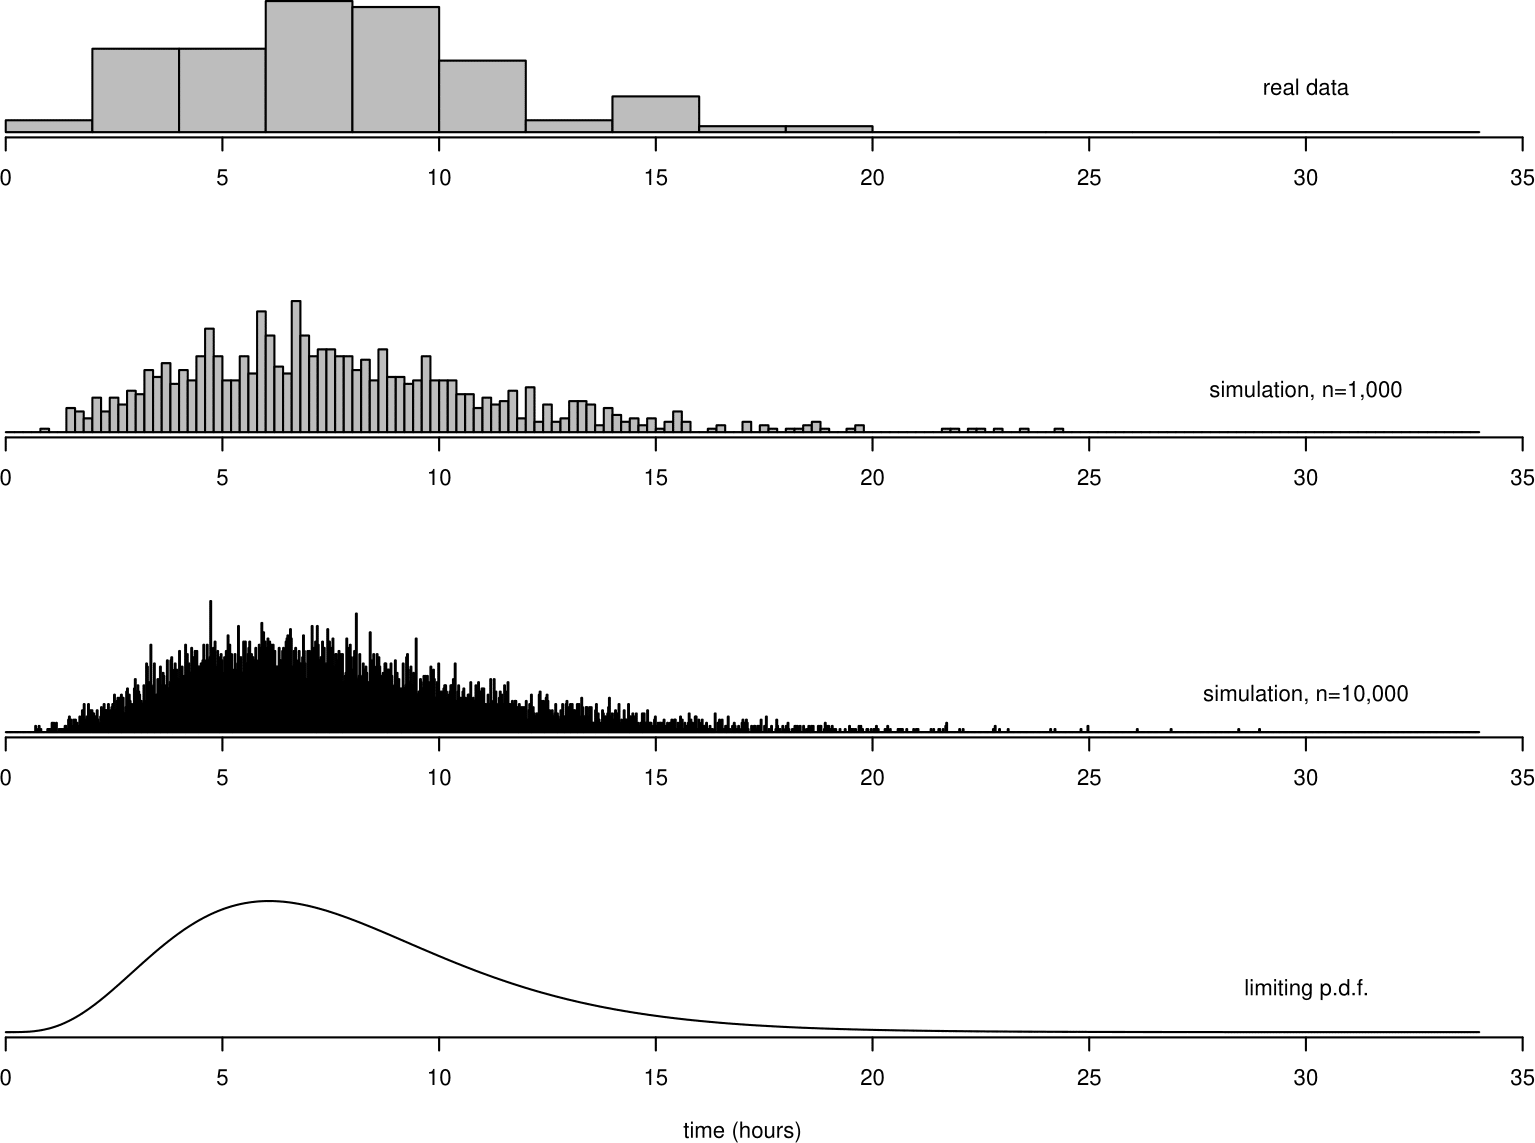
\includegraphics[width=0.75\linewidth]{images/ox_cont_var} 

}

\caption{Top: histogram of the Oxford birth durations. Second from top: histogram of 1,000 values simulated from a distribution fitted to the data. Second from bottom: similarly for 10,000 simulated values. Bottom: p.d.f. of the distribution fitted to the Oxford birth times data.}\label{fig:oxcontvar}
\end{figure}

Suppose that we continue to collect data on birth duration from this hospital, and, as new observations arrive, we add them to the top histogram in Figure \ref{fig:oxcontvar}. We imagine that the times are recorded continuously. As the number of observations \(n\) increases we decrease the bin width of the histogram. As \(n\) increases to infinity the bin width shrinks to zero and the histogram tends to a smooth continuous curve.

This is shown in the bottom 3 plots in Figure \ref{fig:oxcontvar}. The extra data are not real. They are data I have simulated, using a computer, to have a distribution with a similar shape to the histogram of the real data.

Let \(T\) denote the time, in hours, that a woman arriving at the hospital takes to give birth. The smooth continuous curve at the bottom of Figure \ref{fig:oxcontvar} is called the \textbf{probability density function (p.d.f.)} \(f_T(t)\) of the random variable \(T\). Since the total area of the rectangles in a histogram is equal to 1, the area \(\int_{-\infty}^{\infty} f_T(t) \, \mathrm{d}t\) under the p.d.f. \(f_T(t)\) is equal to 1.

\textbf{Definition}. A \textbf{probability density function (p.d.f.)} is a function \(f_{X}(x)\), or simply \(f(x)\), such that

\begin{enumerate}
\def\labelenumi{\arabic{enumi}.}
\tightlist
\item
  \(f_X(x) \geq 0\), for \(-\infty < x < \infty\);
\item
  \(\displaystyle\int_{-\infty}^{\infty} f_X(x) \, \mathrm{d}x = 1\).
\end{enumerate}

Therefore, p.d.f.s are always non-negative and integrate to 1. The support of a continuous random variable is the set of values for which the p.d.f. is positive. Suppose that we wish to find \(P(4 < T \leq 12)\). To find the proportion of times between 4 and 12 using a histogram, we sum the areas of all bins between 4 and 12, that is, we find the area shaded in the histogram in Figure \ref{fig:oxshady}. To do this using the p.d.f. we do effectively the same thing: we find the area under the p.d.f. \(f_T(t)\) between 4 and 12. Since \(f_T(t)\) is a smooth continuous curve, (that is, the bin widths are zero) we integrate \(f_T(t)\) between 4 and 12.

\begin{figure}

{\centering 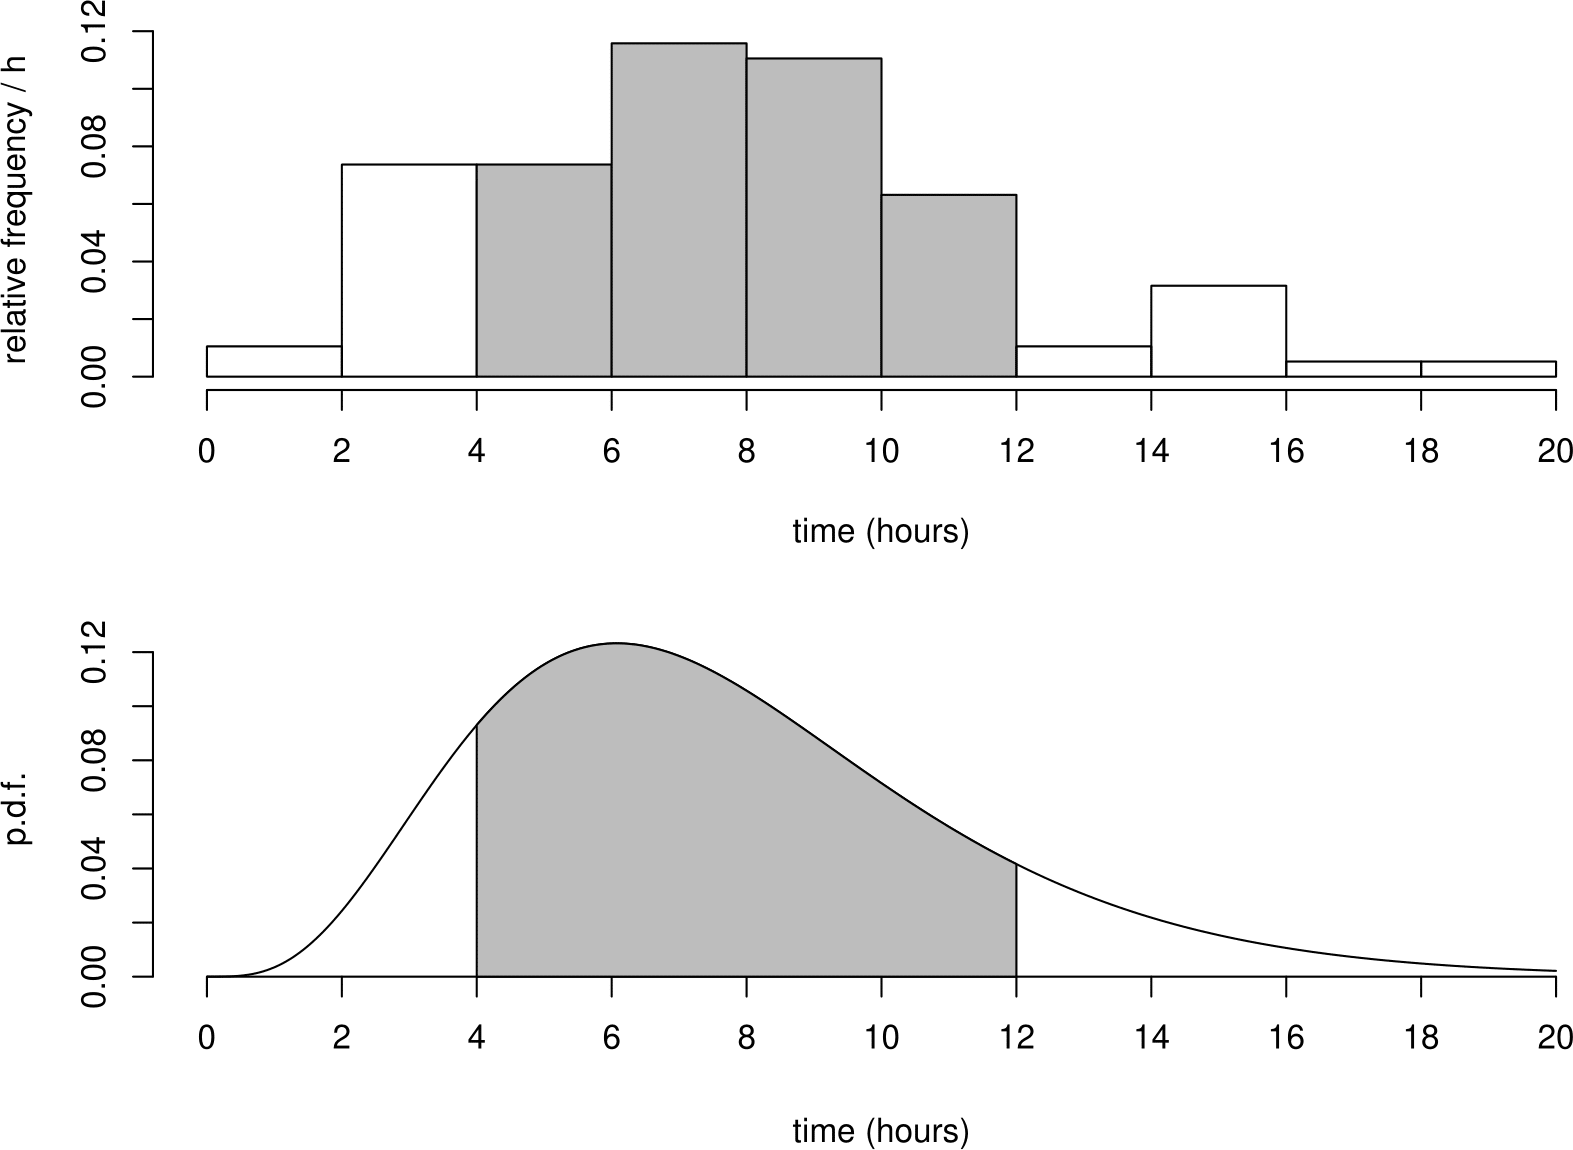
\includegraphics[width=0.75\linewidth]{images/ox_shady} 

}

\caption{Top: histogram of the Oxford birth durations. Bottom: p.d.f. of the distribution fitted to the Oxford birth duration data.}\label{fig:oxshady}
\end{figure}

Therefore
\[ P(4 < T \leq 12) = \displaystyle\int_4^{12} f_T(t) \,\mathrm{d}t = F_T(12)-F_T(4). \]

More generally,
\[ P(a < T \leq b) = \displaystyle\int_a^b f_T(t) \,\mathrm{d}t = F_T(b)-F_T(a). \]

\textbf{Definition}. A random variable \(X\) is a \textbf{continuous random variable} if there exists a p.d.f. \(f_X(x)\) such that
\[
P(a < X \leq b) = \int_{a}^{b} f_X(x) \,\mathrm{d}x,
\]
for all \(a\) and \(b\) such that \(a < b\).

Figure \ref{fig:pdfshady} illustrates the properties of a p.d.f..

\begin{figure}

{\centering 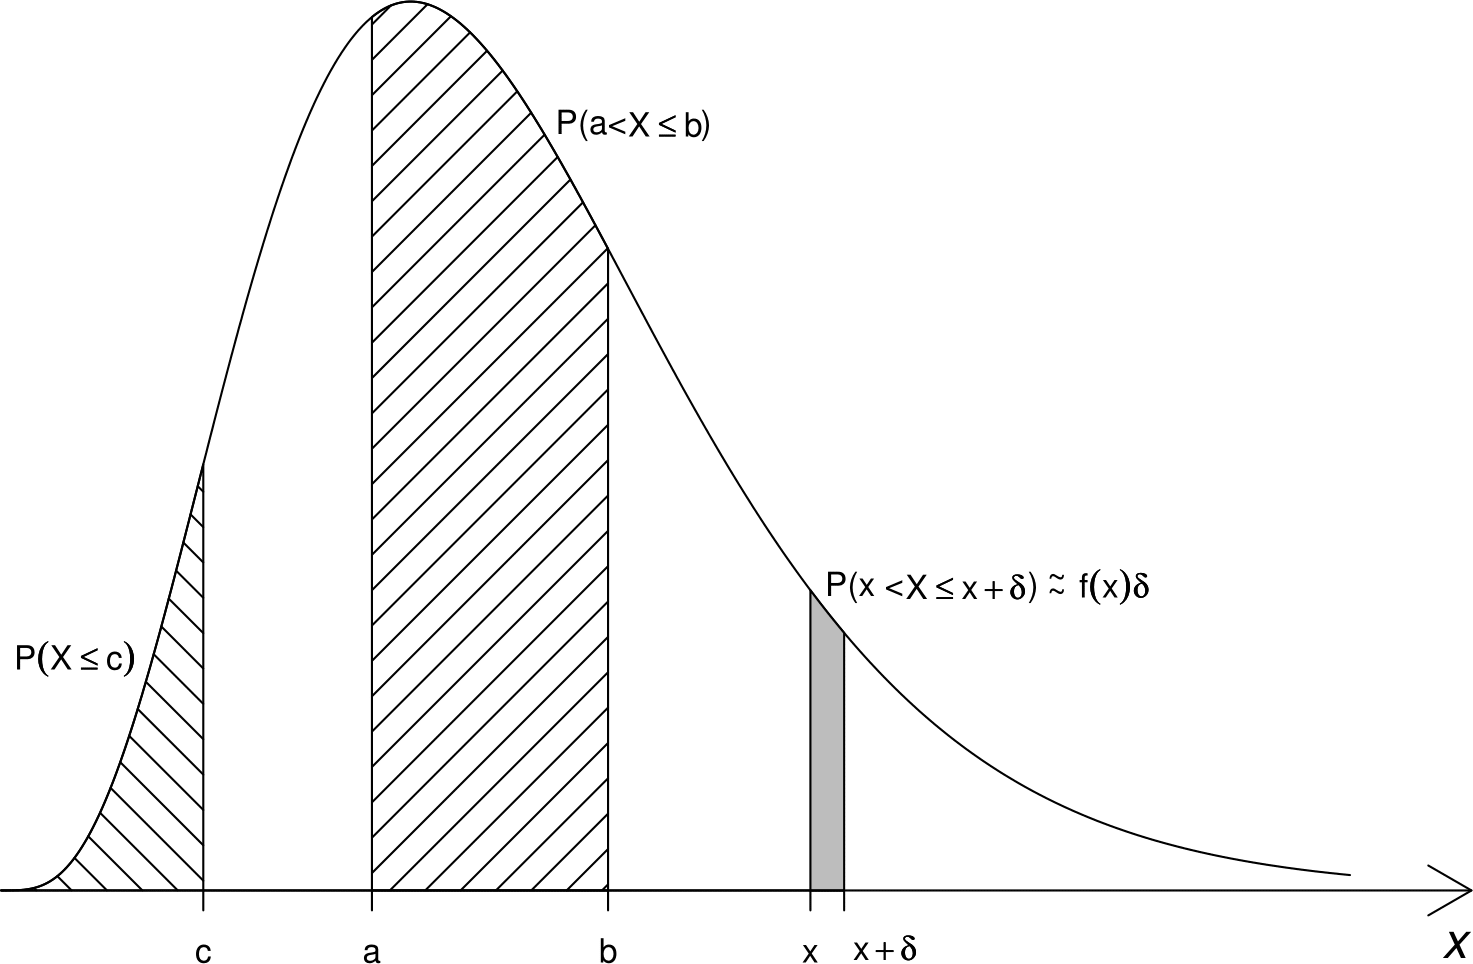
\includegraphics[width=0.75\linewidth]{images/pdf_shady} 

}

\caption{Properties of a p.d.f.. The areas that correspond to the probability that a random variable takes a value in a given interval are shaded.}\label{fig:pdfshady}
\end{figure}

Notes

\begin{itemize}
\tightlist
\item
  It is very important to appreciate that \(f_X(x)\) is \textbf{not} a probability: it does \textbf{not} give \(P(X=x)\). In fact \(P(X=x)=0\): the probability that a continuous random variable \(X\) takes the value \(x\) is zero.
\item
  Indeed, it is possible for a p.d.f. to be greater than 1. Consider a continuous random variable \(X\) with p.d.f.
  \[ f_X(x) = \left\{ \begin{array}{ll} 2\,(1-x) & \,0 \leq x \leq 1, \\ 0 & \,\mbox{otherwise}.\end{array}\right. \]
  For this random variable \(f_X(x)>1\) for any \(x \in [0, 1/2)\) .
\item
  Since \(P(X=x)=0\)
  \[ P(a < X \leq b) = P(a \leq X \leq b) = P(a \leq X < b) = P(a < X < b). \]
\item
  \(f_X(x)\) is a probability \textbf{density}. The probability that \(X\) lies in a very small interval of length \(\delta\) near \(x\) is approximately \(f_X(x) \delta\). For the p.d.f. at the bottom of figure \ref{fig:oxcontvar}, \(f_T(6) > f_T(12)\), indicating that a randomly chosen woman is more likely to spend approximately 6 hours giving birth than approximately
  12 hours.
\end{itemize}

\textbf{Relationship between the c.d.f. and p.d.f. of a continuous random variable}. For a continuous random variable
\[ F_X(x) = P(X \leq x) = \int_{-\infty}^x f_X(u) \,\mathrm{d}u. \]
Therefore,
\[ f_X(x) = \frac{\mathrm{d}}{\mathrm{d}x} F_X(x). \]

\hypertarget{expectation}{%
\section{Expectation}\label{expectation}}

The expectation of a random variable is a measure of the location of its distribution.

\hypertarget{expectation-of-a-discrete-random-variable}{%
\subsection{Expectation of a discrete random variable}\label{expectation-of-a-discrete-random-variable}}

\textbf{Example}. We return to the space shuttle example.

Again we consider test flights conducted at a particular temperature, say 53\(^\circ\)F. Suppose that NASA are able to conduct a very large number \(n\) of test flights at 53\(^\circ\)F, producing a sample \(x_1,\ldots,x_n\) of numbers of damaged O-rings.

Let \(n(x)\) be the number of test flights on which \(x\) of the 6 O-rings were damaged. We can write the sample mean \(\bar{x}\) of \(x_1,\ldots,x_n\) as
\begin{eqnarray*}
\bar{x} &=& \frac{0 \times n(0) + 1 \times n(1) + \cdots + 6 \times n(6)}{n}, \\
&=& \sum_{x=0}^6 x\,\frac{n(x)}{n}.
\end{eqnarray*}
As the sample size \(n\) increases to infinity, the sample proportion \(n(x)/n\) tends to \(P(X=x)\), for \(x=0,1,\ldots,6\). Therefore, in the limit as \(n \rightarrow \infty\), \(\bar{x}\) tends to
\begin{eqnarray}
\sum_{x=0}^6 x\,P(X=x). 
\label{eq:shuttlemean}
\end{eqnarray}
This is known as the mean of the probability distribution of \(X\). It is a measure of the location of the distribution.

The quantity in equation \eqref{eq:shuttlemean} is the value of the sample mean \(\bar{x}\) that we would expect to get from a very large sample. Therefore it is often called the \textbf{expectation} or \textbf{expected value} of the random variable \(X\) and it is denoted \(\mathrm{E}(X)\).

\textbf{Definition}. The \textbf{expectation} (or \textbf{expected value} or \textbf{mean}) \(\mathrm{E}(X)\) of a discrete random variable \(X\) is given by
\begin{eqnarray}
\mathrm{E}(X) &=& \sum_x x\,P(X=x). 
\label{eq:discmean}
\end{eqnarray}
This is a weighted average of the values that \(X\) can take, each value being weighted by \(P(X=x)\).

Note:

\begin{itemize}
\tightlist
\item
  We often write \(\mu\) or \(\mu_X\) for \(\mathrm{E}(X)\).
\item
  Units: the units of \(\mathrm{E}(X)\) are the same as those of \(X\). For example, if \(X\) is measured in hours then \(\mathrm{E}(X)\) is measured in hours.
\item
  \(\mathrm{E}(X)\) exists only if \(\sum_x |x|\,P(X=x) < \infty\). If the number of values \(X\) can take is finite then \(\mathrm{E}(X)\) will always exist.
\end{itemize}

\hypertarget{expectation-of-a-continuous-random-variable}{%
\subsection{Expectation of a continuous random variable}\label{expectation-of-a-continuous-random-variable}}

We can define the expectation of a continuous random variable in a similar way to a discrete random variable, replacing summation with integration.

\textbf{Definition}.
The expectation \(\mathrm{E}(X)\) of a continuous random variable \(X\) is given by
\begin{eqnarray}
\mathrm{E}(X) = \int_{-\infty}^{\infty} x\,f_X(x) \,\mathrm{d}x. 
\label{eq:contmean}
\end{eqnarray}
Note:

\begin{itemize}
\tightlist
\item
  Like the discrete case, this is a weighted average of the values that \(X\) can take, but now each value is weighted by the
  p.d.f. \(f_X(x)\).
\item
  The range of integration in equation \eqref{eq:contmean} is over the whole real line but, in practice, integration will be over the range of possible values of \(X\).
\item
  \(\mathrm{E}(X)\) exists only if \(\int_{-\infty}^{\infty} |x|\,f_X(x) \,\mathrm{d}x < \infty\).
\end{itemize}

\hypertarget{properties-of-mathrmex}{%
\subsection{\texorpdfstring{Properties of \(\mathrm{E}(X)\)}{Properties of \textbackslash mathrm\{E\}(X)}}\label{properties-of-mathrmex}}

If \(a\) and \(b\) are constants then
\[ \mathrm{E}(a\,X+b) = a\,\mathrm{E}(X)+b. \]
This makes sense. If we multiply all observations by \(a\) their mean will also be multiplied by \(a\). If we add \(b\) to all observations their mean will be increased by \(b\), that is, the distribution of \(X\) shifts up by \(b\).

\begin{itemize}
\tightlist
\item
  If \(X \geq 0\) then \(\mathrm{E}(X) \geq 0\).
\item
  If \(X\) is a constant \(c\), that is, \(P(X=c)=1\) then \(\mathrm{E}(X)=c\).
\item
  It can be shown that
  \[ \mathrm{E}(X_1 + X_2 + \cdots + X_n) = \mathrm{E}(X_1) + \mathrm{E}(X_2) + \cdots + \mathrm{E}(X_n). \]
\end{itemize}

\hypertarget{the-expectation-of-gx}{%
\subsection{\texorpdfstring{The expectation of \(g(X)\)}{The expectation of g(X)}}\label{the-expectation-of-gx}}

Suppose that \(Y=g(X)\) is a function of of \(X\), such as \(aX+b\), \(X^2\) or \(\log X\). Then \(Y\) is also a random variable. If we find the p.m.f (if \(Y\) is discrete) or p.d.f. (if \(Y\) is continuous) of \(Y\) then we can find the the expectation of \(Y\) using equation \eqref{eq:discmean} or \eqref{eq:contmean} as appropriate.

\begin{equation}
\mathrm{E}(Y) = \mathrm{E}[g(X)] =
\begin{cases} 
\displaystyle\sum_x g(x)\,P(X=x) & \text{if } X \text{ is discrete}, \\
\int_{-\infty}^{\infty} g(x)\,f_X(x) \,\mathrm{d}x & \text{if } X \text{ is continuous}.
\end{cases}
\label{eq:expfn}
\end{equation}

Note, it is usually the case that
\[ \mathrm{E}[g(X)] \neq g[\mathrm{E}(X)] \]
although there are exceptions.

\hypertarget{variance}{%
\section{Variance}\label{variance}}

The variance of a random variable is a measure of the spread of its distribution.

\hypertarget{variance-of-a-discrete-random-variable}{%
\subsection{Variance of a discrete random variable}\label{variance-of-a-discrete-random-variable}}

\textbf{Example}. We return the space shuttle example.

As before we let \(n(x)\) be the number of test flights on which \(x\) of the 6 O-rings were damaged. We saw in Section \ref{meanstdev} that a measure of the spread of a sample \(x_1,\ldots,x_n\) is the sample variance \(s_X^2\) which, in this example, can be written as

\begin{eqnarray*}
s_X^2 &=& \frac{1}{n-1}\,\left\{
(0-\bar{x})^2\,n(0)+(1-\bar{x})^2\,n(1)+\cdots+(6-\bar{x})^2\,n(6) \right\},
\\
      &=& \sum_{x=0}^6 (x-\bar{x})^2\,\frac{n(x)}{n-1}. 
\end{eqnarray*}
As the sample size \(n\) increases to infinity, \(\frac{n(x)}{n-1}\) tends to \(P(X=x)\), for \(x=0,1,\ldots,6\) and \(\bar{x}\) tends to \(\mu\)=\(\mathrm{E}(X)\).

Therefore, as \(n \rightarrow \infty\), \(s_X^2\) tends to

\begin{equation}
\sum_{x=0}^6 (x-\mu)^2\,P(X=x). 
\label{eq:shuttlevar}
\end{equation}

This is known as the variance of the probability distribution of \(X\). It is a measure of the spread of the distribution. The quantity in equation \eqref{eq:shuttlevar} is the value of the sample variance \(s_X^2\) that we would expect to get from a very large sample.

\textbf{Definition}. The variance \(\mathrm{var}(X)\) of a discrete random variable \(X\) with mean \(\mathrm{E}(X)=\mu\) is given by

\begin{equation}
\mathrm{var}(X) = \sum_x\,(x-\mu)^2\,P(X=x). 
\label{eq:varidisc}
\end{equation}

This is a weighted average of the squared differences between the values that \(X\) can take and its mean \(\mu\), each value being weighted by \(P(X=x)\).

Note:

\begin{itemize}
\tightlist
\item
  \(\mathrm{var}(X)\) exists only if \(\mu\) exists and \(\sum_x (x-\mu)^2\,P(X=x) < \infty\). If the number of values \(X\) can take is finite then \(\mathrm{var}(X)\) will always exist.
\item
  We often write \(\sigma^2\) or \(\sigma_X^2\) for \(\mathrm{var}(X)\).
\end{itemize}

\hypertarget{variance-of-a-continuous-random-variable}{%
\subsection{Variance of a continuous random variable}\label{variance-of-a-continuous-random-variable}}

We can define the variance of a continuous random variable in a similar way to a discrete random variable, replacing summation with integration.

\textbf{Definition}. The variance \(\mathrm{var}(X)\) of a continuous random variable \(X\) with mean \(\mathrm{E}(X)=\mu\) is given by

\begin{equation}
\mathrm{var}(X) = \int_{-\infty}^{\infty} (x-\mu)^2 f_X(x) \,\mathrm{d}x. 
\label{eq:varicont}
\end{equation}

Note: \(\mathrm{var}(X)\) exists only if \(\mu\) exists and \(\int_{-\infty}^{\infty} (x-\mu)^2\,f_X(x) \,\mathrm{d}x < \infty\).

\hypertarget{variance-and-standard-deviation}{%
\subsection{Variance and standard deviation}\label{variance-and-standard-deviation}}

\textbf{Definition}. Let \(X\) be a random variable with \(\mathrm{E}(X)=\mu\). The variance \(\mathrm{var}(X)\) is given by
\[ \mathrm{var}(X) = \mathrm{E}\left[(X-\mu)^2\right]. \]
This follows from equations \eqref{eq:varidisc} and \eqref{eq:varicont} and the expression in equation \eqref{eq:expfn} for the expectation of a function \(g(X)\) of a random variable \(X\).

There is an alternative way to calculate \(\mathrm{var}(X)\):
\[ \mathrm{var}(X) = \mathrm{E}\left(X^2\right) - [\mathrm{E}(X)]^2. \]

\textbf{Exercise}. Prove this.

\textbf{Definition}. The standard deviation sd\((X)\) of \(X\) is given by sd(\(X\))=\(+\sqrt{\mathrm{var}(X)}\).

Notes on \(\mathrm{var}(X)\):

\begin{itemize}
\tightlist
\item
  \(\mathrm{var}(X) \geq 0\). A variance cannot be negative.\\
\item
  Units: the units of \(\mathrm{var}(X)\) are the square of those of \(X\). For example, if \(X\) is measured in hours then \(\mathrm{var}(X)\) is measured in hours\(^2\) (and sd(\(X\)) is measured in hours).
\end{itemize}

\hypertarget{properties-of-mathrmvarx}{%
\subsection{\texorpdfstring{Properties of \(\mathrm{var}(X)\)}{Properties of \textbackslash mathrm\{var\}(X)}}\label{properties-of-mathrmvarx}}

\begin{itemize}
\tightlist
\item
  If \(a\) and \(b\) are constants then
  \[ \mathrm{var}(a\,X+b) = a^2\,\mathrm{var}(X). \]
  This makes sense. If we multiply all observations by \(a\) their variance, which is measured square units, will be multiplied by \(a^2\). If we add \(b\) to all observations their variance will be unchanged because the distribution simply shifts up by \(b\) and its spread is unaffected.
\item
  If \(X\) is a constant \(c\), that is, \(P(X=c)=1\) then \(\mathrm{var}(X)=0\): the distribution of \(X\) has zero spread.
\item
  It can also be shown that \textbf{if the random variables \(X_1, X_2, \ldots X_n\) are independent} then
\end{itemize}

\begin{equation}
\mathrm{var}(X_1 + X_2 + \cdots + X_n) = \mathrm{var}(X_1) + \mathrm{var}(X_2) + \cdots + \mathrm{var}(X_n). 
\label{eq:varsum}
\end{equation}

\textbf{Note}. Independence is sufficient for this result to hold but it is not necessary. Taking \(n=2\) as an example, in generality we have
\[ \mathrm{var}(X_1 + X_2) = \mathrm{var}(X_1) + \mathrm{var}(X_2) + 2\,\mathrm{cov}(X_1,X_2), \]
where \(\mathrm{cov}(X_1,X_2)\) is the \textbf{covariance} between the random variables \(X_1\) and \(X_2\). Covariance is a measure of the strength of \textbf{linear} association. If \(X_1\) and \(X_2\) are independent (have no association of any kind) then \(\mathrm{cov}(X_1,X_2)=0\), because they have no linear association. However, it is possible for \(X_1\) and \(X_2\) to be dependent but \(\mathrm{cov}(X_1,X_2)=0\), because, although they have some kind of association, they have no \textbf{linear} association. Thus, independence is a stronger requirement than zero covariance.

Returing to general \(n\) we have
\[ \mathrm{var}(X_1 + X_2 + \cdots + X_n) = \mathrm{var}(X_1) + \mathrm{var}(X_2) + \cdots + \mathrm{var}(X_n) + 2 \mathop{\sum\sum}_{i < j} \mathrm{cov}(X_i,X_j). \]
If \(\mathrm{cov}(X_i,X_j)=0\) for all \(i < j\) then equation \eqref{eq:varsum} holds. We will study covariance, and its standardised form \textbf{correlation}, in Chapter \ref{correlationchapter}.

\hypertarget{locations}{%
\section{Other measures of location}\label{locations}}

\hypertarget{the-median-of-a-random-variable}{%
\subsection{The median of a random variable}\label{the-median-of-a-random-variable}}

Recall that the sample median of a set of observations is the middle observation when the observations are arranged in order of size. We define the median of a random variable \(X\) as the value, median(\(X\)), such that

\[ P(X < \mathrm{median}(X)) \leq \frac12 \leq P(X \leq \mathrm{median}(X)). \]

In other words, \(\mathrm{median}(X)\) is the value where a plot of the c.d.f. \(F_X(x)=P(X \leq x)\) crosses \(1/2\).

For a continuous random variable \(X\) we have
\[  F_X(\mathrm{median}(X)) = P(X \leq \mathrm{median}(X)) =\frac12. \]
and the median will divide the distribution into two parts, each with probability 1/2:
\[ P(X < \mathrm{median}(X)) = P(X > \mathrm{median}(X)) = \frac12. \]

This will not necessarily hold for a discrete distribution. For example, suppose that
\[ P(X=0)=\frac16, \qquad  P(X=1)=\frac12, \qquad P(X=2)=\frac13. \]

Then
\begin{eqnarray*}
F_X(x) = P(X \leq x) = \left\{\begin{array}{ll}
0 & \mbox{for } x <0, \\
\frac16 & \mbox{for } 0 \leq x < 1, \\
\frac23 & \mbox{for } 1 \leq x < 2, \\
1 & \mbox{for } x \geq 2, 
\end{array}\right.
\end{eqnarray*}
Therefore, \(\mathrm{median}(X) = 1\). However, \(P(X<1)=\frac16\) and \(P(X>1)=\frac13\).

\hypertarget{the-mode-of-a-random-variable}{%
\subsection{The mode of a random variable}\label{the-mode-of-a-random-variable}}

Recall that the sample mode of categorical or discrete data is the value (or values) which occurs most often. We define the mode, mode(\(X\)), of a random variable as follows.

For a discrete random variable \(X\), the mode is the value which has the highest probability of occurring: \(P(X=\mathrm{mode}(X))\) will be larger than for any other value \(X\) can have. In other words, \(\mathrm{mode}(X)\) is the value at which the p.m.f. is maximised.

For a continuous random variable \(X\), the mode is the value at which the p.d.f. is maximised. \textbf{If the maximum occurs at a turning point of \(f_X(x)\)} then it can be found by solving the equation
\[ \frac{\mathrm{d}}{\mathrm{d}x} f_X(x)  = 0, \]
and checking that you have indeed found a maximum.

\hypertarget{quantiles}{%
\section{Quantiles}\label{quantiles}}

To keep things simple we consider a \textbf{continuous} random variable \(X\). The \(100p\%\) quantile of \(X\) is defined to be the value \(x_p\) such that
\[ F_X(x_p)=P(X \leq x_p) = p. \]
Thus, \(x_{1/4}\) is the lower quartile of \(X\), \(x_{1/2}\) is the median of \(X\) and \(x_{3/4}\) is the upper quartile of \(X\). The inter-quartile range is \(x_{3/4}-x_{1/4}\), which is a measure of spread.

\hypertarget{measures-of-shape}{%
\section{Measures of shape}\label{measures-of-shape}}

The \textbf{moment coefficient of skewness} of a random variable \(X\) with mean \(\mu\) and standard deviation \(\sigma\) is given by
\[ \mathrm{E}\left[\left(\frac{X - \mu}{\sigma}\right)^3\right] = \displaystyle\frac{\mathrm{E}\left[\left(X- \mu\right)^3\right]}{\sigma^3}, \]
provided that \(\mathrm{E}[\left(X- \mu\right)^3]\) exists.

The \textbf{quartile skewness} of a random variable \(X\) with c.d.f \(F_X(x)\) is given by
\[ \frac{[F_X(3/4) - F_X(1/2)] - [F_X(1/2) - F_X(1/4)]}{F_X(3/4) - F_X(1/4)}. \]

\hypertarget{simple}{%
\chapter{Simple distributions}\label{simple}}

In this section we use a dataset to introduce some commonly-used simple distributions. We will study the \textbf{discrete} distributions: Bernoulli, binomial, geometric and Poisson. We will also study the \textbf{continuous} distributions: uniform, exponential, normal.

\hypertarget{the-bernoulli-distribution}{%
\section{The Bernoulli distribution}\label{the-bernoulli-distribution}}

\hypertarget{binomial}{%
\section{The binomial distribution}\label{binomial}}

\hypertarget{the-geometric-distribution}{%
\section{The geometric distribution}\label{the-geometric-distribution}}

\hypertarget{the-poisson-distribution}{%
\section{The Poisson distribution}\label{the-poisson-distribution}}

\hypertarget{the-uniform-distribution}{%
\section{The uniform distribution}\label{the-uniform-distribution}}

\hypertarget{the-exponential-distribution}{%
\section{The exponential distribution}\label{the-exponential-distribution}}

\hypertarget{normal}{%
\section{The normal distribution}\label{normal}}

\hypertarget{qq-plots}{%
\section{QQ plots}\label{qq-plots}}

\hypertarget{statistical-inference}{%
\chapter{Statistical Inference}\label{statistical-inference}}

\hypertarget{sample-and-populations}{%
\section{Sample and populations}\label{sample-and-populations}}

\hypertarget{probability-models}{%
\section{Probability models}\label{probability-models}}

\hypertarget{fitting-models}{%
\section{Fitting models}\label{fitting-models}}

\hypertarget{uncertainty-in-estimation}{%
\section{Uncertainty in estimation}\label{uncertainty-in-estimation}}

\hypertarget{good}{%
\section{What makes an estimator good?}\label{good}}

\hypertarget{assessing-goodness-of-fit}{%
\section{Assessing goodness-of-fit}\label{assessing-goodness-of-fit}}

\hypertarget{contingency}{%
\chapter{Contingency tables}\label{contingency}}

\hypertarget{way2}{%
\section{2-way contingency tables}\label{way2}}

\hypertarget{comparing-probabilities}{%
\subsection{Comparing probabilities}\label{comparing-probabilities}}

Note that in Ross, S. (2010) A First Course in Probability the odds ratio of an event \(A\) is defined (incorrectly) as \(P(A) / (1 - P(A))\). This is a ratio of probabilities. The conventional use of the term \textbf{odds ratio} is for a ratio of odds.

\hypertarget{way3}{%
\section{3-way contingency tables}\label{way3}}

\hypertarget{linreg}{%
\chapter{Linear regression}\label{linreg}}

\hypertarget{simple-linear-regression}{%
\section{Simple linear regression}\label{simple-linear-regression}}

\hypertarget{looking-at-scatter-plots}{%
\section{Looking at scatter plots}\label{looking-at-scatter-plots}}

\hypertarget{model-checking}{%
\section{Model checking}\label{model-checking}}

\hypertarget{outliers}{%
\subsection{Outliers and influential observations}\label{outliers}}

\hypertarget{linregtrans}{%
\section{Use of transformations}\label{linregtrans}}

\hypertarget{over-fitting}{%
\section{Over-fitting}\label{over-fitting}}

\hypertarget{other-aspects-of-regression}{%
\section{Other aspects of regression}\label{other-aspects-of-regression}}

\hypertarget{uncertainty-in-parameter-estimates}{%
\section{Uncertainty in parameter estimates}\label{uncertainty-in-parameter-estimates}}

\hypertarget{correlationchapter}{%
\chapter{Correlation}\label{correlationchapter}}

\hypertarget{correlation-a-measure-of-linear-association}{%
\section{Correlation: a measure of linear association}\label{correlation-a-measure-of-linear-association}}

\hypertarget{covariance-and-correlation}{%
\section{Covariance and correlation}\label{covariance-and-correlation}}

\hypertarget{use-and-misuse-of-correlation}{%
\section{Use and misuse of correlation}\label{use-and-misuse-of-correlation}}

\hypertarget{a-general-strategy-for-statistical-modelling}{%
\chapter{A general strategy for statistical modelling}\label{a-general-strategy-for-statistical-modelling}}

  \bibliography{book.bib,packages.bib}

\end{document}
